\documentclass[a4paper]{article}

\def\npart {S\&DS 410/610}
\def\nlecturer {Zhou Fan}
\def\ncourse {Statistical Inference}
\def\nauthor{Leqi Xu \footnote{If you find any typos, please email them to leqi.xu@yale.edu. Many thanks to Tianyu Liu for pointing out previous typos.}}
\def\nyear {2021}
\def\nterm {Fall}
\def\nofficial {http://www.stat.yale.edu/~zf59/stats_410_610/schedule.html}

\input{header}

\begin{document}
	\maketitle

\section*{Main Topics in Statistical Inference}

{	\noindent\textbf{Unit I: Finite sample theory}
	
	\vspace{10pt}
	\noindent\textbf{Exponential family models}\\
	Natural parameters and sufficient statistics. Cumulant generating function $A(\eta)$, moments and cumulants of $T(x)$.\hspace*{\fill} [3]
	
	\vspace{10pt}
	\noindent\textbf{Sufficiency, minimal sufficiency and Rao-Blackwell}\hspace*{\fill} [1]
	
	\vspace{10pt}
	\noindent\textbf{Decision theory and optimality of estimators}\\
	Admissibility and domination. Bayesian paradigm: average risk with respect to prior, posterior distributions, Bayes estimator and Bayes risk. Minimax paradigm: worst-case risk, Bayes risk as lower bounds, least favorable priors.\hspace*{\fill} [4]
	
	\vspace{10pt}
	\noindent\textbf{High dimensions (Gaussian sequence model)}\\
	Shrinkage estimation, James-Stein estimation, Stein's Lemma and Stein's unbiased estimator for risk. Sparsity, soft thresholding and hard thresholding\hspace*{\fill} [2]
	
	\vspace{10pt}
	\noindent\textbf{Hypothesis testing}\\
	Type I and type II error. Simple v.s. simple tests, likelihood ratio and Neyman-Pearson Lemma. Uniformly most power tests, average power v.s. worst-case power. Gaussian sparse model: sparse v.s. dense alternatives to $\theta = 0$. Multiple testing, false discovery rate, Bonferroni procedure and Holm's procedure.\hspace*{\fill} [4]
	
	\vspace{15pt}
	\noindent\textbf{Unit II: Asymptotic theory}
	
	\vspace{10pt}
	\noindent\textbf{Basic tools}\\
	Weak Law of large Numbers. Central Limit Theorem. Slutsky's Lemma. Continuous Mapping Theorem. Delta Method.\hspace*{\fill} [2]
	
	\vspace{10pt}
	\noindent\textbf{Maximum likelihood estimation and point-wise asymptotics}\\
	Asymptotic consistency, uniform convergence and covering net. Asymptotic normality, efficiency of maximum likelihood estimation and Taylor expansion of log-likelihood.\hspace*{\fill} [3]
	
	\vspace{10pt}
	\noindent\textbf{Local asymptotics}\\
	Testing, contiguity and local asymptotic normality of log-likelihood. Asymptotic power under local alternatives and 3 likelihood-based tests.Limiting normal experiment, efficiency and superefficiency of estimators.\hspace*{\fill} [6]}

\tableofcontents

\setcounter{section}{0}

\section*{Unit 1 Finite Sample Theory}
\addcontentsline{toc}{section}{Unit 1 Finite Sample Theory}
\markboth{Unit 1 Finite Sample Theory}{Unit 1 Finite Sample Theory}

\begin{eg*}
	Suppose $X_1,X_2,\cdots X_n \stackrel{\text{i.i.d.}}{\sim} N(\theta,1)$. How to estimate $\theta$? \\
	The ``obvious" answer is the sample mean
	\begin{equation*}
		\bar{X} = \frac{X_1+X_2+\cdots+X_n}{n}.
	\end{equation*}
	We can measure error by \emph{loss function}
	\begin{equation*}
		L(\bar{X},\theta) = (\bar{X} - \theta)^2.
	\end{equation*}
	This is random. We can take the expected value, called the \emph{risk}
	\begin{equation*}
		R(\bar{X},\theta) = \mathbb{E}_{\theta}\left[(\bar{X}-\theta)^2\right] = \frac{1}{n}.
	\end{equation*}
\end{eg*}

\begin{eg*}
	Suppose $X_1,X_2,\cdots X_n \stackrel{\text{i.i.d.}}{\sim} N(\theta,1)$, $Y_1,Y_2,\cdots,Y_n \stackrel{\text{i.i.d.}}{\sim} N(\mu,1)$, $Z_1,Z_2,\cdots,Z_n \stackrel{\text{i.i.d.}}{\sim} N(\nu,1)$. How to estimate $(\theta,\mu,\nu)$? \\
	The ``obvious" answer is the sample mean
	\begin{equation*}
		(\bar{X},\bar{Y},\bar{Z}) = \left(\frac{X_1+X_2+\cdots+X_n}{n},\frac{Y_1+Y_2+\cdots+Y_n}{n},\frac{Z_1+Z_2+\cdots+Z_n}{n}\right).
	\end{equation*}
	Total squared error risk is
	\begin{equation*}
		R\left((\bar{X},\bar{Y},\bar{Z}),(\theta,\mu,\nu)\right) = \mathbb{E}_{\theta,\mu,\nu}\left[(\bar{X}-\theta)^2+(\bar{Y}-\mu)^2+(\bar{Z}-\nu)^2\right] =\frac{3}{n}.
	\end{equation*}
	\begin{thm*}(Stein '56, '61)
		There exists an estimate $(\delta_X,\delta_Y,\delta_Z)$ which is \emph{uniformly} better than $(\bar{X},\bar{Y},\bar{Z})$
		\begin{equation*}
			R\left((\delta_X,\delta_Y,\delta_Z),(\theta,\mu,\nu)\right) < \frac{3}{n} \text{ for \emph{every} } (\theta,\mu,\nu).
		\end{equation*}
	\end{thm*}
	\noindent One such estimator is
	\begin{equation*}
		(\delta_X,\delta_Y,\delta_Z) = \left(1-\frac{1}{n(\bar{X}^2+\bar{Y}^2+\bar{Z}^2)}\right)(\bar{X},\bar{Y},\bar{Z}).
	\end{equation*}
	The improvement is the biggest when $(\theta,\mu,\nu) = (0,0,0)$. This is called the ``Stein's Paradox" -- Efron, Morris.
\end{eg*}

\begin{question*}
	In what sense is $\bar{X}$ a ``good" estimate of $\theta$?
\end{question*}

\begin{answer*}
	\quad 
	\begin{itemize}
		\item Gauss: 
		\begin{itemize}
			\item Among all possible $\theta$, $\theta = \bar{X}$ maximizes the probability of data. (Maximum likelihood -- developed by Fisher, 1912-1922). 
			\item $\bar{X}$ is unbiased: $\mathbb{E}_{\theta}[\bar{X}] = \theta$. It minimizes $R(\bar{X},\theta)$ among all linear, unbiased estimators. (In fact, it's true among \emph{all} unbiased estimators).
		\end{itemize}
		\newpage
		\item Fisher, Neyman, Pearson, Wald, $\cdots$ : 
		\begin{itemize}
			\item Sufficiency: All ``information" about $\theta$ is contained in $\bar{X}$. By Rao-Blackwell, if $\delta_X$ is another estimator, not a function of $\bar{X}$, then there exists $\delta_X^{'}$ such that
			\begin{equation*}
				R(\theta,\delta_X^{'}) < R(\theta,\delta_X) \quad \forall \theta.
			\end{equation*}
			\item Minimax: Using Bayesian techniques, for any estimator $\delta_X$
			\begin{equation*}
				\frac{1}{n} = \sup_{\theta \in \mathbb{R}} R(\theta,\bar{X}) \leq \sup_{\theta \in \mathbb{R}} R(\theta,\delta_X).
			\end{equation*}
			\item Admissibility: Using Bayesian techniques, there does \emph{not} exist estimator $\delta_X$ such that
			\begin{equation*}
				R(\theta,\delta_X) < R(\theta,\bar{X}) \quad \forall \theta \in \mathbb{R}.
			\end{equation*}
			(Holds in dimensions $1$ or $2$, not $\geq 3$).
			\item local asymptotic normality: as $n \to \infty$, this normal model is a ``good approximation" for many other parametric models.
		\end{itemize}
	\end{itemize}
\end{answer*}

\begin{defi*}
	A \emph{statistical model} is a family of probability distributions $p$ over a sample space $\mathcal{X}$. Most of this class index $p$ by a \emph{parameter} $\theta$ belonging to a parameter space $\Omega: \mathcal{P} = \{P_{\theta} \in \Omega \}$.
\end{defi*}

\noindent \textbf{Goal:} Use data from $p_{\theta}$ to draw conclusions about $\theta$.
\begin{itemize}
	\item Point estimation: Estimate $\theta$ or a function $g(\theta)$.
	\item Hypothesis testing: Does $\theta$ belong to $\Omega_0 \subset \Omega$ or to $\Omega_1 \subset \Omega_1$?
	\item Uncertainty quantification: What is a set or interval to which $\theta$ belongs?
\end{itemize}

\begin{center}
	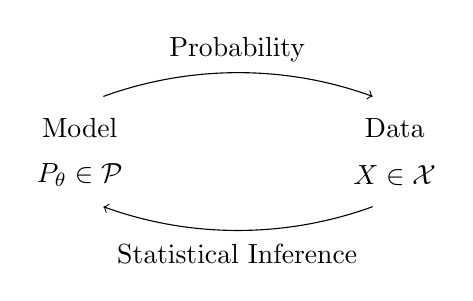
\begin{tikzpicture}
		\node (a1)at(-2,0.3){Model};
		\node (a2)at(2,0.3){Data};

		\node (b1)at(-2,-0.3){$P_\theta \in \mathcal{P}$};
		\node (b2)at(2,-0.3){$X \in \mathcal{X}$};
		
		\node (c1)at(0,1.3){Probability};
		\node (c2)at(0,-1.3){Statistical Inference};
		
		\draw [->] (-1.7,0.7) arc(110:70:5);
		\draw [<-] (-1.7,-0.7) arc(-110:-70:5);
	\end{tikzpicture}
\end{center}

\noindent \textbf{Not covered:} Design experiments, choice of models, diagnostics for model fit.

\section{Preparations}

\subsection{Measure and Integral}
\textbf{Goal:} To define a common language to describe continuous and discrete models.

\begin{defi}[Measure]
	A \emph{measure} $\mu$ on $\mathcal{X}$ assigns non-negative values (possibly 0, $\infty$) to subsets $A \subset \mathcal{X}$ such that
	\begin{enumerate}
		\item if $A$ and $B$ are disjoint, then 
		\begin{equation}
			\mu(A \cup B) = \mu (A) + \mu(B).
		\end{equation}
		\item if $\left\{A_i\right\}_{i = 1}^{\infty}$ are disjoint, then
		\begin{equation}
			\mu\left(\bigcup\limits_{i = 1}^{\infty}A_i\right) = \sum\limits_{i = 1}^{\infty}\mu(A_i).
		\end{equation} 
	\end{enumerate}
\end{defi}

\begin{eg}
	For finite or countable $\mathcal{X},$ $\mu$ is called a \emph{counting measure} on $\mathcal{X}$ if
	\begin{equation}
		\mu (A) =\left\{ 
		\begin{array}{ll}
			\text{number of elements in }A & A\text{ is finite} \\
			\infty & A\text{ is infinite.}
		\end{array} \right.
	\end{equation}
\end{eg}


\begin{eg}
	Suppose $\mathcal{X}=\mathbb{R}$. Then there exists a unique measure $\mu$ on a large class of subsets (Borel $\sigma$-algebra) of $\mathcal{X}$ such that
	\begin{equation}
		\mu\left((a,b)\right) = b-a.
	\end{equation}
In this case, $\mu$ is called the \emph{Lebesgue measure} on $\mathcal{X}$.
\end{eg}

\begin{remark}
	\quad
	\begin{enumerate}
		\item If $\mathcal{X}$ is finite or countable, we can define $\mu$ for \emph{all subsets} of $\mathcal{X}$.
		\item If $\mathcal{X} = \mathbb{R}$, we can only define $\mu$ on a class of subsets $\mathbbm{t}$ such that
		\begin{enumerate}
			\item $\emptyset, \mathcal{X} \in \mathbbm{t},$
			\item If $A \in \mathbbm{t}$, then $A^c \in \mathbbm{t},$
			\item If $A_1, A_2, A_3, \cdots \in \mathbbm{t}$, then $\sum\limits_{i = 1}^{\infty} A_i \in \mathbbm{t}$. $\mathbbm{t}$ is called a \emph{$\sigma$-algebra}.
		\end{enumerate}
	
	\end{enumerate}
	The \emph{Borel $\sigma$-algebra} is the smallest $\sigma$-algebra containing all open (and closed) subsets of $\mathcal{X}$. These sets are the \emph{measurable sets}.
\end{remark}

\begin{eg}
	Suppose $\mathcal{X}=\mathbb{R}^n$, then there exists a unique measure $\mu$ on the Borel $\sigma$-algebra $\mathbbm{t}$, which is the Lebesgue measure, that satisfies for any  $(a_i, b_i) \subset \mathbbm{t}, \ i = 1,2, \cdots, n $
	\begin{equation}
		\mu \left((a_1, b_1) \times (a_2, b_2) \times \cdots \times (a_n, b_n)\right) = \prod\limits_{i = 1}^{n} (b_i - a_i).
	\end{equation}
	\newpage
	\noindent Associated to every measure $\mu$ is a model of defining an integral on $\mathcal{X}$:
	\begin{enumerate}
		\item $f: \mathcal{X} \to \mathbb{R}$ is \emph{simple} if it takes only a finite number of values $\left\{a_1, a_2, \cdots, a_k\right\}$ on $\left\{A_1, A_2, \cdots, A_k\right\}$, then
		\begin{equation}
			\int f(x) \d \mu (x) = \sum\limits_{i = 1}^{k} a_i \cdot \mu (A_i).
		\end{equation}
		\item If $f_1, f_2, \cdots$ are simple, non-negative functions and $f_i(x) \nearrow f(x)$ for any $x \in \mathcal{X}$, then
		\begin{equation}
			\int f(x) \d \mu (x) = \lim\limits_{i \rightarrow \infty} \int f_i(x) \d \mu (x) \quad (\text{possibly } \infty).
		\end{equation}
		\item For arbitary $f: \mathcal{X} \to \mathbb{R}$, let $f^+(x) = \max (f(x), 0), f^-(x) = -\min(f(x), 0)$ (Check: $f(x) = f^+(x) - f^-(x)$).If
		\begin{equation*}
			\int f^+(x) \d \mu (x) < \infty,\ \int f^-(x) \d \mu (x) < \infty \iff \int \abs{f(x)} \d \mu (x) <  \infty,
		\end{equation*}
		then $f$ is \emph{integrable}, and
		\begin{equation}
			\int f(x) \d \mu (x) = \int f^+(x) \d \mu (x) - \int f^-(x) \d \mu (x).
		\end{equation}
	\end{enumerate}
\end{eg}

\begin{remark}
	For arbitary functions $f$, where $f^+, f^-$ can be described by (iii) in the above example is called \emph{measureable functions}.
\end{remark}

\begin{eg}
	If $\mathcal{X}$ is finite or countable, $\mu$ is the counting measure, then
	\begin{equation}
		\int f(x) \d \mu (x) = \sum\limits_{x \in \mathcal{X}} f(x).
	\end{equation}
	And $f \text{ is integrable} \iff \sum\limits_{x \in \mathcal{X}} \abs{f(x)} < \infty$.
\end{eg}

\begin{eg}
	Suppose $\mathcal{X}=\mathbb{R}$ and $\mu$ is the Lebesgue measure, then for ``nice" functions, this is the usual integral for calculations
	\begin{equation}
		\int f(x) \d \mu (x) = \int f(x) \d x.
	\end{equation}
	Similarly for the integral in $\mathbb{R}^n.$
\end{eg}

\begin{eg}
	Let $(\mathcal{X}, \mu)$ be any space, $A \subset \mathcal{X}$ be any (measurable) set. Let $\mathbbm{1}_A = \left\{
	\begin{array}{ll}
		1 & x \in A \\
		0 & x  \notin A
	\end{array}
	\right.,$ then $\int \mathbbm{1}_A (x) \d \mu (x) = \mu (A)$. Write
	\begin{equation}
		\int_A f(x) \d \mu (x) = \int \mathbbm{1}_A \cdot f(x) \d \mu (x).
	\end{equation}
	And if $\mathcal{X} \text{ is countable, then} \int_A f(x) \d \mu (x) = \sum\limits_{x \in A} f(x)$.
\end{eg}

\newpage
\begin{prop} Basic properties of integral are the followings: 
		\begin{enumerate}
			\item Linearity: 
			\begin{equation}
				\int c \cdot f(X) \d \mu (x) = c \cdot \int f(x) \d \mu (x),
			\end{equation}
			\begin{equation}
				\int \left(f(x) + g(x)\right) \d \mu (x) = \int f(x) \d \mu (x) + \int g(x) \d \mu (x)).
			\end{equation}
			\item If $f \geq 0$, then
			\begin{equation}
				\int f(x) \d \mu \geq 0.
			\end{equation}
			If $f (x) \geq g(x)$, then
			\begin{equation}
				\int f(x) \d \mu (x) \geq \int g(x) \d \mu (x).
			\end{equation}
			\item Suppose $N \subset \mathcal{X},\ \mu (N) = 0$ and $f(x) = g(x) \text{ for any } x \notin N,$ then we say $f = g$ is \emph{almost everywhere (a.e.)}. Then 
			\begin{equation}
				\int f(x) \d \mu (x) = \int g(x) \d \mu (x).
			\end{equation}
		\end{enumerate}
\end{prop}


\begin{prop}Less basic properties of integral are the followings:
	Suppose $f_1, f_2, \cdots: \mathcal{X} \to \mathbb{R}$ satisfy $f_i(x) \to f(x) \text{ for any } x \in \mathcal{X}.$ The following is not always true
	 \begin{equation}
		 \int f_i(x) \d \mu = \lim\limits_{i \to \infty} \int f_i(x) \d \mu (x).
	 \end{equation}
\end{prop}

\begin{eg}
	Suppose $\mathcal{X}$ is $\mathbb{R}$ and $\mu$ is the Lebesgue measure. $f_i(x) = \left\{
	\begin{array}{ll}
		i & x \in (0, \frac{1}{i}) \\
		0 & \text{otherwise}
	\end{array}
	\right.,$ Then $\int f_i(x) \d \mu (x) = 1 \text{ for any } i$, But $f_i(x) \to f(x) \equiv 0 \text{ for any } x \in \mathbb{R}$ and $\int f(x) d \mu (x) = 0,$ so
	\begin{equation}
		\int \lim\limits_{i \to \infty} f_i (x) \d \mu (x) \neq \lim\limits_{i \to \infty} \int f_i (x) \d \mu (x).
	\end{equation}
\end{eg}

\begin{lemma}[Fatou's lemma]
	If $f_1, f_2, \cdots \geq 0$ then
	\begin{equation}
	\lim\limits_{i \to \infty} \int f_i (x) \d \mu (x) \geq \int (\lim\limits_{i \to \infty} f_i (x)) \d \mu (x).
	\end{equation}
\end{lemma}

\begin{thm}[Monotone Convergence Theorem]
	If $f_1, f_2, \cdots \geq 0$ and $f_i(x) \nearrow f(x) \text{ for any } x \in \mathcal{X}$, then
	\begin{equation}
		\lim\limits_{i \to \infty} \int f_i (x) \d \mu (x) = \int f(x) \d \mu (x) \quad (\text{possibly } \infty).
	\end{equation}
\end{thm}

\begin{thm}[Dominated Convergence Theorem]
	If $f_i (x) \to f(x) \ \text{ for any } x \in \mathcal{X}$ and $\exists g: \mathcal{X} \to \mathbb{R}$ such that $\abs{f_i(x)} \leq g(x) \text{ for any } i, x$ and $\int g(x) \d \mu (x) < \infty$, then
	\begin{equation}
		\lim\limits_{i \to \infty} \int f_i (x) \d \mu (x) = \int f(x) \d \mu (x).
	\end{equation}
\end{thm}

\subsection{Probability and Densities}

\begin{eg}
	Let $X$ be a random variable taking value in $\mathcal{X}$. The fraction $P^x (A) = \mathbb{P} [x \in A]$ is a measure, called the \emph{distribution} or \emph{law} of $x$.
\end{eg}

\begin{defi}[Probability measure]\index{probability measure}
	A \emph{probability measure} $\mu$ on $\mathcal{X}$ is a measure such that $\mu(\mathcal{X}) = 1$.
\end{defi}
 
 \begin{defi}[Density function]\index{density function}
 For any space $(\mathcal{X}, \mu)$ and function $p: \mathcal{X} \to [0, \infty), \upsilon (A) = \int_A p(x) \d \mu (x) = \int p(x) \mathbbm{1}_A (x) \d \mu (x)$ defines a new measure on $\mathcal{X}$. $p(x)$ is the \emph{density function} of $\upsilon$ with respect to $\mu$.
 \end{defi}

\begin{eg}
	If $\mathcal{X}$ is countable, and X is a ``discrete" random variable on $\mathcal{X}$ with law $P^x$. The \emph{probability mass function} $p(x) = \mathbb{P}[X = x]$ is the density of $P^x$ with respect to counting measure $\mu$ and
	\begin{equation}
		P^x (A) = \mathbb{P} [X \in A] = \sum\limits_{x \in A} \mathbb{P} [X = x]= \int_A p(x) \d \mu (x) 
	\end{equation}
\end{eg}

\begin{eg}
	If $\mathcal{X}$ is $\mathbb{R}$ or $\mathbb{R}^n$, $X$ is a ``continuous" random variable on $\mathcal{X}$ with law $\mathbb{P}^x$. The \emph{probability density function} is the density of $P^x$ with respect to Lebesgue measure $\mu$ and
	\begin{equation}
		P^x (A) = \mathbb{P}[X \in A] = \int_A p(x) \d x = \int_A p(x) \d \mu (x).
	\end{equation}
\end{eg}

\begin{prop}
	If $\upsilon$ has density $p(x)$ with respect to $\mu$, then
	\begin{equation}
		\int g(x) \d \upsilon (x) = \int g(x)p(x) \d \upsilon (x).
	\end{equation}
\end{prop}

\begin{proof}
	This is the proof where $g$ is simple. Let $g(x) = \sum\limits_{i = 1} ^k a_i \mathbbm{1}_{A_i} \upsilon (A_i) (x)$, then
	\begin{equation}
		\begin{aligned}
			\int g(x) \d \upsilon(x) &= \sum\limits_{i = 1}^k a_i \int \mathbbm{1}_{A_i} (x) \d \upsilon(x)\\
			&= \sum\limits_{i = 1}^k a_i \upsilon (A_i)\\
			&= \sum\limits_{i = 1}^k a_i \int_{A_i} p(x) \d \mu (x)\\
			& = \int \sum\limits_{i = 1}^k a_i \mathbbm{1}_{A_i} (x) p(x) \d \mu (x)\\
			& = \int g(x)p(x) \d \mu (x).
		\end{aligned}
	\end{equation}
\end{proof}

\begin{defi}[Expection]\index{expectation}
	If $X$ is a random variable on $\mathcal{X}$, \emph{expectation} with respect to $X$ is integration with respect to $P^x$.
\end{defi}

\begin{eg}
	\quad
	\begin{enumerate}
		\item If $X$ is discrete, then
		\begin{equation}
			\mathbb{E} [T(X)] = \int T(x) \d P^x (x) = \int T(x) p(x) \d \mu (x) = \sum\limits_{x \in \mathcal{X}} T(x)p(x).
		\end{equation}
		\item If $X$ is continuous, then
		\begin{equation}
			\mathbb{E} [T(X)] = \int T(x) \d P^x (x) = \int T(x) p(x) \d x.
		\end{equation}
	\end{enumerate}
\end{eg}

\subsection{Exponential Family Models}
\textbf{Recall:} A statistical model $\mathcal{P} = \{P_\theta: \theta \in \omega\}$ is a family of probability distributions on the sample space $\mathcal{X}$.

\begin{defi}[Domination]\index{domination}
	$\mathcal{P}$ is \emph{dominated} by a common measure $\mu$ if each $P_{\theta}$ admits a density with respect to $\mu$.
\end{defi}

\begin{note}
	For us, $\mu$ is usually the counting or Lebesgue measure.
\end{note}

\begin{defi}[Identifiability]\index{identifiability}
	$\theta$ is \emph{identifiable} if $\theta_1 \neq \theta_2$ implies $P_{\theta_1} \neq P_{\theta_2}.$
\end{defi}

\begin{defi}[Exponential family model]\index{exponential family model}
	$\{P_{\theta}: \theta \in \Omega\}$ are an \emph{exponential family model} if they have densities of the form
	\begin{equation}
		p_{\theta} (x) = \exp\left(\sum\limits_{i = 1}^s {\eta}_i (\theta) T_i (x) - B(\theta)\right)h(x),
	\end{equation}
	with respect to a common measure $\mu$.
	${\eta}_1, \eta_2, \cdots, {\eta}_s$ are called \emph{natural parameters}, $T_1, T_2, \cdots, T_s$ are called the \emph{sufficient statistics}. $e^{B(\theta)}$ is the normalizing constant:
	\begin{equation}
		e^{B(\theta)} = \int \exp\left(\sum\limits_{i = 1}^s {\eta}_i (\theta) T_i (x)\right)h(x) \d \mu (x).
	\end{equation}
\end{defi}

\begin{eg}
	For Binomial($n, \theta$) model, where $n$ is fixed and known, densities:
	\begin{equation*}
		\begin{aligned}
			p_{\theta}(x) &= \binom{n}{x} {\theta}^x {(1-\theta)}^{n-x} \\
			&= \binom{n}{x}\exp \left(x\log(\theta) + (n-x)\log(1-\theta)\right)\\
			& = \binom{n}{x} \exp \left(x\log\left(\frac{\theta}{1 - \theta}\right) + n\log(1 - \theta)\right).
		\end{aligned}
	\end{equation*}
	Here, we can have different representation (1.3.1) for the density. For example,
	\begin{enumerate}
		\item $h(x) = \binom{n}{x}, T_1 (x) = x, {\eta}_1 (\theta) = \log (\theta), T_2 (x) = n-x, {\eta}_2 (\theta) = \log(1 - \theta), B(\theta) = 0.$
		\item $h(x) = \binom{n}{x}, T_1 (x) = x, {\eta}_1 (\theta) = \log \left(\frac{\theta}{1 - \theta}\right), B(\theta) = -n\log (1 - \theta).$
	\end{enumerate}
\end{eg}

\newpage
\begin{remark}
	\quad
	\begin{enumerate}
		\item The representation (1.3.1) is not unique.
		\item (1.3.1) is \emph{minimal} if neither ${\eta}_1, \eta_2, \cdots, {\eta}_s$ nor $T_1, T_2, \cdots, T_s$ obey any linear relations. Otherwise, the number of terms $s$ in (1.3.1) can be reduced.
	\end{enumerate}
\end{remark}

\begin{eg}
	For $N(\mu, {\sigma}^2)$ model, $\theta = (\mu, {\sigma}^2) \in \mathbb{R} \times (0, \infty)$, densities:
	\begin{equation*}
		\begin{aligned}
			p_{\theta} (x) &= \frac{1}{\sqrt{2 \pi {\sigma}^2}} \exp \left(- \frac{(x - \mu)^2}{2 {\sigma}^2}\right) \\
			&= \exp\left(-\frac{1}{2{\sigma}^2} x^2 + \frac{\mu}{{\sigma}^2}x - \frac{{\mu}^2}{2 {\sigma}^2} - \frac{1}{2} \log (2 \pi {\sigma}^2)\right).
		\end{aligned}
	\end{equation*}
	Here, $\eta_1 (\theta) = -\frac{1}{2{\sigma}^2}, T_1(x) = x^2, \eta_2 (\theta) = \frac{\mu}{{\sigma}^2}, T_2(x) = x, b(\theta) =  \frac{{\mu}^2}{2 {\sigma}^2} + \frac{1}{2} \log (2 \pi {\sigma}^2)$.
\end{eg}

\noindent Oftentimes, it is convenient to reparametrize by $\eta_1, \eta_2 \cdots, \eta_s$:
\begin{equation}
	p(x|\eta) = \exp \left(\sum\limits_{i = 1}^s \eta_i T_i (x) - A(\eta)\right)h(x).
\end{equation}
This is called \emph{canonical form}. $A(\eta)$ is the \emph{log-partition function}(a.k.a., \emph{cumulant generating function}, \emph{free energy}). $e^{A(\eta)}$ is the \emph{partition function}.
\begin{equation}
	e^{A(\eta)} = \int \exp\left(\sum\limits_{i = 1}^s \eta_i T_i (x)\right)h(x) \d \mu (x).
\end{equation}

\begin{eg}
	According to (1.3.1), $Binomial(n, \theta)$ model has densitites:
	\begin{equation*}
		p_\theta(x) = \binom{n}{x} \exp \left(x\log\left(\frac{\theta}{1 - \theta}\right) + n\log(1 - \theta)\right),
	\end{equation*}
	and we reparametrize it by $\eta = \log\left(\frac{\theta}{1 - \theta}\right)$, which is the \emph{logit} transform. Then $\frac{\theta}{1 - \theta} = e^{\eta}, \theta = \frac{e^{\eta}}{1+e^{\eta}}, \log(1-\theta) = \log\left(\frac{1}{1+e^{\eta}}\right) = -\log(1 + e^{\eta})$, so
	\begin{equation}
		p(x|\eta) = \exp (\eta x - n\log(1+e^{\eta}))\binom{n}{x}.
	\end{equation}
	Here, $T_1(x) = x, A(\eta) = n\log(1+e^{\eta}), h(x) = \binom{n}{x}.$\\
	This is well-defined for all $\eta \in \mathbb{R}$, so $\mathbb{R}$ is called the natural parameter space.
\end{eg}

\begin{defi}[Natural parameter space]\index{natural parameter space}
	The \emph{natural parameter space} is 
	\begin{equation}
		\Xi = \left\{\eta \in \mathbb{R}^s: \int \exp \left(\sum\limits_{i = 1}^s \eta_i T_i (x)\right)h(x) \d \mu (x) < \infty\right\}.
	\end{equation}
	This is the largest set of natural parameters under which the model is well-defined.
\end{defi}

\begin{eg}
	According to (1.3.2), $N(\mu,{\sigma}^2)$ model, $\theta = (\mu, {\sigma}^2)$ has densities:
	\begin{equation*}
		p_\theta(x) = \exp\left(-\frac{1}{2{\sigma}^2} x^2 + \frac{\mu}{{\sigma}^2}x - \frac{{\mu}^2}{2 {\sigma}^2} - \frac{1}{2} \log (2 \pi {\sigma}^2)\right).
	\end{equation*}
	Set $\eta_1 = -\frac{1}{2{\sigma}^2}, \eta_2 = \frac{\mu}{{\sigma}^2}$, then ${\sigma}^2 = -\frac{1}{2\eta_1}, \mu = -\frac{\eta_2}{2\eta_1}$, so
	\begin{equation}
		p(x|\eta) = \exp \left(\eta_1 x^2 + \eta_2 x + \frac{{\eta_2}^2}{2\eta_1}-\frac{1}{2}\log\left(-\frac{\pi}{\eta_1}\right)\right).
	\end{equation}
	Note: $\int e^{\eta_1 x^2 + \eta_2 x} \d x < \infty \iff \eta_1 < 0$.\\
	So $\Xi = (-\infty,0) \times \mathbb{R}$.
\end{eg}

\begin{eg}
	Multinomial($n; p_0, p_1, \cdots, p_s$) model on $s+1$ possible outcomes. Here, $\mathcal{X} = \left\{(x_0, x_1, \cdots, x_s): 0 \leq x_0 \leq x_1, \cdots, x_s \leq n, \sum\limits_{i = 0}^s x_i = n\right\}, \theta = (p_0, p_1, \cdots, p_s)$, then
	\begin{equation}
		\begin{aligned}
			p_{\theta} (x) &= \binom{n}{x_0, x_1, \cdots, x_s} p_0^{x_0} p_1^{x_1} \cdots p_s^{x_s} \\
			&= \binom{n}{x_0, x_1, \cdots, x_s} \exp\left(\sum\limits_{i = 1}^s x_i \log(p_i) + (n - x_1 - x_2 - \cdots - x_s \log(p_0))\right) \\
			&= \binom{n}{x_0, x_1, \cdots, x_s} \exp\left(\sum\limits_{i = 1}^s x_i \log\left(\frac{p_i}{p_0}\right) + n\log(p_0)\right) \\
		\end{aligned}
	\end{equation}
	Set $\eta_i = \log\left(\frac{p_i}{p_0}\right), i = 1, 2, \cdots, s$, then $e^{\eta_i} = \frac{p_i}{p_0}$.
	We have $p_0 + p_1 + \cdots + p_s = p_0(1+e^{\eta_1}+e^{\eta_2}+\cdots+e^{\eta_s}) = 1$, so $p_0 = \frac{1}{1+e^{\eta_1}+e^{\eta_2}+\cdots+e^{\eta_s}}$, then
	\begin{equation}
		p(x|\eta) = \binom{n}{x_0, x_1, \cdots, x_s} \exp\left(\sum\limits_{i = 1}^s \eta_i x_i - n\log(1+e^{\eta_1}+e^{\eta_2}+\cdots+e^{\eta_s})\right)\quad.
	\end{equation}
	So $\Xi = \mathbb{R}^s$.
\end{eg}

\begin{eg}
	For Gamma($a,b$) model, $\mathcal{X} = (0, \infty)$, then
	\begin{equation}
		\begin{aligned}
			p_\theta(x) &= \frac{1}{\Gamma (a) b^a} x^{a-1}e^{-\frac{x}{b}}\\
			&=\exp \left(a \log (x) - \frac{1}{b} x -\log(\Gamma (a))- a \log (b)\right) \frac{1}{x}.
		\end{aligned}
	\end{equation}
	Set $\eta_1 = a, \eta_2 = -\frac{1}{b}$, then
	\begin{equation}
		p(x|\eta) = \exp(\eta_1\log(x)+\eta_2x-\log(\Gamma(\eta_1))+\eta_1\log(-\eta_2))\frac{1}{x}.
	\end{equation}
	Note:$\int_{0}^{\infty} \exp (\eta_1\log(x) + \eta_2x) \frac{1}{x}dx = \int_{0}^{\infty} x^{\eta_1 -1} e^{\eta_2x}dx < \infty \iff \eta_2<0, \eta_1 > 0$.
	So $\Xi = (0, \infty) \times (\infty,0).$
\end{eg}


\begin{note*} There are three important inequalities that we can use in the proof:
\begin{itemize}
	\item Cauchy-Schwarz inequality: Let $\mu$ be the probability measure, $f,g: R \rightarrow R$:
	\begin{equation*}
	\begin{aligned}
		& \int f(x) g(x) d \mu(x) \leq\left[\int f(x)^{2} d \mu(x)\right]^{1 / 2}\left[\int g(x)^{2} d \mu(x)\right]^{1 / 2}. \\
        & \E[f(x) g(x)] \leq \sqrt{\E\left(f(x)^{2}\right)} \sqrt{\E\left(g(x)^{2}\right)}.	
	\end{aligned}
	\end{equation*}	
	\item Hölder's inequality: for any measure $\upsilon$, any non-negative functions $f,g: \mathcal{X} \to [0,\infty)$, and any $\alpha,\beta > 1$ such that $\frac{1}{\alpha}+\frac{1}{\beta} = 1$, then
	\begin{equation*}
		\int f(x)g(x) \d \upsilon (x) \leq \left(\int {f(x)}^{\alpha} \d \upsilon\right)^{\frac{1}{\alpha}}\left(\int {g(x)}^{\beta} \d \upsilon\right)^{\frac{1}{\beta}}.
	\end{equation*}	
	\item Jensen’s inequality: Let $\mu$ be the probability measure, for a random variable $X$ and a convex function $f: R \rightarrow R$: 
	\begin{equation*}
	\begin{aligned}
		& f \left(\int x d \mu(x) \right) \leq \int f(x) d \mu(x). \\
		& f \left(\E [X] \right) \leq \E[ f \left( X \right)].
	\end{aligned}
	\end{equation*}	
\end{itemize}
\end{note*}

\begin{prop}
	The natural parameter space $\Xi$ is always convex.
\end{prop}

\begin{proof}
	Recall: $\Xi$ is convex if
	\begin{equation*}
		x, y \in \Xi \implies \lambda x + (1-\lambda)y \in \Xi \quad \forall \lambda \in (0,1).
	\end{equation*}
	Let $\eta = (\eta_1,\eta_2,\cdots,\eta_s) \in \Xi, \ \eta' = (\eta_1',\eta_2',\cdots,\eta_s') \in \Xi$. Fix $\lambda \in (0,1)$. \\
	\newline
	By Hölder's inequality: For any measure $\upsilon$, any non-negative functions $f,g: \mathcal{X} \to [0,\infty)$, and any $\alpha,\beta > 1$ such that $\frac{1}{\alpha}+\frac{1}{\beta} = 1$, then
	\begin{equation}
		\int f(x)g(x) \d \upsilon (x) \leq \left(\int {f(x)}^{\alpha} \d \upsilon\right)^{\frac{1}{\alpha}}\left(\int {g(x)}^{\beta} \d \upsilon\right)^{\frac{1}{\beta}}.
	\end{equation}
	\noindent Apply (1.3.12) to $\upsilon(A) = \int_A h(x) \d \mu (x), \ f(x) = \exp\left(\sum\limits_{i = 1}^s \lambda \eta_i T_i(x)\right), \ g(x) = \exp\left(\sum\limits_{i = 1}^s (1 - \lambda)\eta_i' T_i (x)\right), \ \alpha = \frac{1}{\lambda}, \ \beta = \frac{1}{1-\lambda}$, then:
	\begin{equation}
		\begin{aligned}
			&\int \exp \left(\sum\limits_{i = 1}^s(\lambda \eta_i + (1-\lambda) \eta_i')T_i (x)\right)h(x) \d \mu (x) \\
			&= \int f(x)g(x) \d \upsilon (x) \\
			& \leq \left(\int {f(x)}^{\alpha} \d \upsilon\right)^{\frac{1}{\alpha}}\left(\int {g(x)}^{\beta} \d \upsilon\right)^{\frac{1}{\beta}} \\
			&= \left(\int \exp\left(\sum\limits_{i = 1}^s \eta_i T_i(x)\right) h(x) \d \mu (x)\right)^{\lambda} \left(\int \exp\left(\sum\limits_{i = 1}^s \eta_i' T_i (x)\right) h(x) \d \mu (x)\right)^{1 - \lambda} \\
			&< \infty.
		\end{aligned}
	\end{equation}
	So $\lambda \eta + (1-\lambda)\eta' \in \Xi$.
\end{proof}

\begin{remark}
	A specific problem might restrict the parameter space to be a smaller (possibily non-convex) subset of $\Xi$.
\end{remark}

\begin{eg}
	For the normal model that we restrcit mean = st.dev. $N(\theta, {\theta}^2) \ \theta > 0$. It has densities:
	\begin{equation*}
		p_{\theta} (x) = \exp \left(-\frac{1}{2{\theta}^2} x^2 + \frac{1}{\theta} x - \frac{1}{2} - \frac{1}{2} \log(2 \pi {\theta}^2)\right).
	\end{equation*}
	This representation is minimal since there are no linear relations. \\ Here, $(\eta_1, \eta_2) = (-\frac{1}{2{\theta}^2}, \frac{1}{\theta})$. Parameter space: ${\left(\eta_1, \eta_2\right) \in \Xi: \eta_2 > 0. \eta_1 = - \frac{1}{2} {\eta_2}^2}$. \\ These examples are sometimes called ``curved" exponential families.
\end{eg}

\begin{prop}
	$A(\eta)$ is convex.
\end{prop}

\begin{proof}
	Recall: $A(\eta)$ is convex if $\eta, \eta' \in \Xi \implies \lambda \eta + (1-\lambda) \eta' \in \Xi \quad \forall \lambda \in (0,1)$.\\
	\begin{equation}
		\begin{aligned}
			&A(\lambda \eta + (1-\lambda) \eta') \\
			&= \log\left[\int \exp \left(\sum\limits_{i = 1}^s(\lambda \eta_i + (1-\lambda) \eta_i')T_i (x)\right)h(x) \d \mu (x)\right] \\
			&\leq \log\left[\left(\int \exp\left(\sum\limits_{i = 1}^s \eta_i T_i(x)\right) h(x) \d \mu (x)\right)^{\lambda} \left(\int \exp\left(\sum\limits_{i = 1}^s \eta_i' T_i (x)\right) h(x) \d \mu (x)\right)^{1 - \lambda}\right] \\
			&= \lambda A(\eta) + (1-\lambda) A(\eta').
		\end{aligned}
	\end{equation}
\end{proof}

\begin{question}
	Why are exponential families useful?
\end{question}

\begin{answer}
	\quad
	\begin{enumerate}
		\item Defining generalized linear models. 
		\begin{eg}[Logistic regression]
			Let $X_i\sim{Bernoulli(p_i)},i = 1,2,\cdots n$. The natural parameters are $\eta_i = \log(\frac{p_i}{1-p_i}),i = 1,2,\cdots n$. Model these by a linear model, $\eta_i = \alpha + \beta z_i$ for observed \emph{covariates} $z_1, z_2, \cdots,z_n$. \\
			More generally, for many 1-parameter family $X_i\sim{p(x|\eta_i)}$, model $\eta_i = \alpha + \beta z_i$. This is called using the \emph{canonical link function}. The advantages are concave log-likelihood and finite number of sufficient statistics.
	  	\end{eg}
		 \item In Bayesian inference, we place a \emph{prior} $p(\eta)$ on $\eta$ and we use \emph{posterior} $p(\eta | x)$. Certain forms for $p(\eta)$ are called conjugate priors, which lead to simple forms for $p(\eta | x)$ in the same family as $p(\eta)$. For $\eta$ as the canonical parameter in exponential families, there is always a conjugate prior.
		 \item Useful way of extending simpler statistical models.
		\begin{eg}[Random graphs]
			Let $\mathcal{X} = \left\{ \text{graphs on n vertices,} \right.\\ \left.\text{ represented by } x_1, x_2, \cdots, x_{\binom{n}{s}} \in \{0,1\}  \right\}$. The simple model is Erdos-Renyi graph where edges are Bernoulli($\theta$). Set $\eta = \log(\frac{\theta}{1-\theta}),$
			\begin{equation}
		 		\begin{aligned}
		 		\ p(x|\eta) &= \prod \limits_{i = 1}^{\binom{n}{2}} \exp(x_i \eta - \log(1+e^{\eta}))\\
		 			&= \exp\left(\eta \cdot \text{(number of edges)} - \binom{n}{2}\log(1+e^{\eta})\right).
		 		\end{aligned}
			\end{equation}
			In reality, we may want to capture more features such as the number of triangles or 4-cliques in the network. Let $T_1(x) = \text{number of edges}, \ T_2(x) = \text{number of triangles}, \ T_3(x) = \text{number of 4-cliques}$. Consider the model
			\begin{equation}
				p(x|\eta) = \exp(\eta_1 T_1(x) + \eta_2 T_2(x) + \eta_3 T_3(x) - A(\eta)).
			\end{equation}
		 	This model contains Erdos-Renyi as special case ($\eta_2 = \eta_3 = 0$). Varients $\eta_2$, $\eta_3$ encourage or discourage the number of triangles or 4-cliques. This is called an \emph{exponential random graph model} (ERGM).\\
		 	Note: $A(\eta)$ typically lacks a closed form expression, and is hard to compute.
		 	\begin{equation}
		 		A(\eta) = \log \left(\sum_{i \in \{0,1\}^{\binom{n}{2}}} \exp(\eta_1 T_1(x) + \eta_2 T_2(x) + \eta_3 T_3(x))\right)
			\end{equation} 
 	   	 \end{eg}
		 \item Minimize Kullback–Leibler divergence. Consider a ``simple" distribution $P$ for the data with density $p$. And we want to find the closest distribution $Q$ such that $E_{Q}[T_i(x)] = t_i \quad \forall i = 1,2, \cdots , s$ for some fixed values $t_1, t_2, \cdots t_s$ and certain statistics $T_1, T_2, \cdots T_s$. Let
		\begin{equation}
			D_{KL}(Q||P) = \int q(x)\log\left(\frac{q(x)}{p(x)}\right) \d \mu (x),
		\end{equation}
	 	the Kullback–Leibler divergence. Our goal is to find $Q$ which minimizes $D_{KL}(Q||P)$ such that  $E_{Q}[T_i(x)] = t_i \quad \forall i = 1,2, \cdots , s$.
	 	\begin{claim}
		 	Under mild assumptions, $Q$ belongs to exponential family.
		\end{claim}
	 	\begin{proof}
	 		Proof sketch: Introduce Lagrange multipliers.\\
	 		Goal: 
	 		\begin{equation*}
	 			\begin{aligned}
	 				& \min\limits_{Q: E_Q[T_i(x)] = t_i \ \forall i} \{D_{KL}(Q||P)\} \\
	 				&=\min\limits_{Q} \max\limits_{\eta_1, \eta_2, \cdots, \eta_s \in \mathbb{R}} \left\{D_{KL}(Q||P) + \sum\limits_{i=1}^s \eta_i(t_i - E_Q[T_i(x)])\right\}
	 			\end{aligned}
	 		\end{equation*}
 			\noindent If $Q$ satisfies mild convex density conditions
	 		\begin{equation*}
	 			\begin{aligned}
	 				\text{Goal} &=\max\limits_{\eta_1, \eta_2, \cdots, \eta_s \in \mathbb{R}} \min\limits_{Q} \left\{D_{KL}(Q||P) + \sum\limits_{i=1}^s \eta_i(t_i - E_Q[T_i(x)])\right\} \\
	 				&=\max\limits_{\eta_1, \eta_2, \cdots, \eta_s \in \mathbb{R}} \left\{\sum\limits_{i=1}^s \eta_i t_i + \min\limits_{Q} \left\{D_{KL}(Q||P) - \sum\limits_{i=1}^s \eta_i E_Q[T_i(x)] \right\} \right\} \\
	 				&=\max\limits_{\eta_1, \eta_2, \cdots, \eta_s \in \mathbb{R}} \left\{\sum\limits_{i=1}^s \eta_i t_i + \min\limits_{Q} \int \left\{ \log(\frac{q(x)}{p(x)}) - \sum\limits_{i=1}^s \eta_i T_i(x) \right\} q(x) \d \mu (x) \right\}.
				\end{aligned}
			\end{equation*}
			Let $p_{\eta} (x) = \exp\left(\sum\limits_{i = 1}^{s} \eta_i T_i(x) - A(\eta)\right)p(x)$. \\
			Then $\log(p_{\eta} (x)) = \sum\limits_{i = 1}^{s} \eta_i T_i(x) + \log(p(x)) -  A(\eta))$.
 			\begin{equation}
 				\begin{aligned}
 					& \max\limits_{\eta_1, \eta_2, \cdots, \eta_s \in \mathbb{R}} \left\{\sum\limits_{i=1}^s \eta_i t_i + \min\limits_{Q} \int \left\{ \log(\frac{q(x)}{p(x)}) - \sum\limits_{i=1}^s \eta_i T_i(x) \right\} q(x) \d \mu (x) \right\} \\
 					&= \max\limits_{\eta_1, \eta_2, \cdots, \eta_s \in \mathbb{R}} \left\{\sum\limits_{i=1}^s \eta_i t_i + \min\limits_{Q} \int \left\{ \log(q(x)) - \log(p_{\eta} (x)) -A(\eta) \right\} q(x)\d \mu (x) \right\} \\
 					&= \max\limits_{\eta_1, \eta_2, \cdots, \eta_s \in \mathbb{R}} \left\{\sum\limits_{i=1}^s \eta_i t_i -A(\eta) + \min\limits_{Q} \int \left\{ \log\frac{q(x)}{p_{\eta} (x)}\right\} q(x)\d \mu (x) \right\} \\
 					&= \max\limits_{\eta_1, \eta_2, \cdots, \eta_s \in \mathbb{R}} \left\{\sum\limits_{i=1}^s \eta_i t_i -A(\eta) + \min\limits_{Q} D_{KL}(Q || p_\eta)\right \}.
 				\end{aligned}
 			\end{equation}
 		Since $D_{KL}(Q || p_\eta) > 0$, we need $Q = P_\eta$ and $\eta$ maxmizes $ \sum\limits_{i=1}^s \eta_i t_i -A(\eta)$.
	 	\end{proof}
 		\item If $x_1, x_2, \cdots, x_n \stackrel{\text{i.i.d.}}{\sim} P_{\eta}$, where $P_{\eta}(x_i)$ are exponential family models $p_{\eta}(x_i) = \exp(\sum\limits_{j=1}^s \eta_j T_j(x_i) - A(\eta))h(x_i)$. then
 		\begin{equation}
 			\begin{aligned}
 				p(x_1, x_2, \cdots, x_n|\eta) 
 				&= \prod\limits_{i = 1}^n \exp\left(\sum\limits_{j=1}^s \eta_j T_j(x_i) - A(\eta)\right)h(x_i) \\
 				&= \exp\left\{\sum\limits_{j=1}^s \eta_j\left(\sum\limits_{i=1}^n T_j(x_i) - n A(\eta)\right)\right\}\prod\limits_{i = 1}^n h(x_i).
 			\end{aligned}
 		\end{equation}
 		This is still an exponential family model on the space $\mathcal{X}^n$ with same number of sufficient statistics which are now $\sum\limits_{i=1}^n T_j(x_i)$ for $j = 1,2, \cdots s$.
	\end{enumerate}
\end{answer}

\subsection{Moments and Cumulants}
\textbf{Recall:} An exponential family model $\mathcal{P}={\P_\theta:\theta \in \Omega}$ has the densities
\begin{equation*}
	p_{\theta}(x) = \exp\left(\sum\limits_{i=1}^s \eta_i(\theta)T_i(x)-b(\theta)\right)h(x)
\end{equation*}
with respect to a common measure $\mu$. It's often convenient to reparametrize by $\eta_1,\eta_2,\cdots,\eta_s$;
\begin{equation*}
	p(x|\eta) = \exp\left(\sum\limits_{i=1}^s \eta_i T_i(x) - A(\eta)\right) h(x).
\end{equation*}
Here, $e^{A(\eta)} = \int \exp\left(\sum\limits_{i=1}^s \eta_i(\theta)T_i(x)-b(\theta)\right)h(x) \d \mu(x)$ is the \emph{partition function}. $A(\eta)$ is the \emph{log-partition function} (a.k.a., \emph{cumulant generating function}, \emph{free energy}).

\begin{defi}[Moment generating function]\index{moment generating function}
	The \emph{moment generating function} of a real-valued random variable $T$ is $M_T(u) = \mathbb{E}[e^{u T}]$.
\end{defi}

\begin{prop} If $M_T(u) < \infty$ for any $u \in (-\delta,\delta)$ for some $\delta > 0$, then
	\begin{enumerate}
		\item For all $\mu \in (-\delta,\delta), \ k \geq 1$,
		\begin{equation}
			\frac{d^k}{du^k}M_T(u) = \mathbb{E}\left[T^ke^{uT}\right] \text{ and } \mathbb{E}\left[\abs{T}^ke^{uT}\right] < \infty
		\end{equation}
		\item If $\mathbb{E}\left[\abs{T}^k\right] < \infty$ for any $k \geq 0$, then the Taylor expansion of $M_T(u)$ around $u = 0$ is
		\begin{equation}
			M_t(u) = 1 + \left(\mathbb{E}\left[T\right]\right)u + \left(\mathbb{E}\left[T^2\right]\right)\frac{u^2}{2} + \left(\mathbb{E}\left[T^3\right]\right)\frac{u^3}{6} + \cdots
		\end{equation}
	\end{enumerate}
\end{prop}

\begin{proof}
	Applying (i) at $u = 0$ yields (ii). To show (i)
	\begin{itemize}
		\item For $k = 1$,
		\begin{equation*}
			\begin{aligned}
				\frac{d}{du}M_T(u) &= \lim\limits_{h \to 0} \frac{M_T(u+h) - M_T(u)}{h} \\
				&= \lim\limits_{h \to 0} \frac{\mathbb{E}\left[e^{(u+h)T}\right] - \mathbb{E}\left[e^{uT}\right]}{h} \\
				&= \lim\limits_{h \to 0} \int \frac{e^{ut}(e^{ht}-1)}{h}dP^T(t). \\
			\end{aligned}
		\end{equation*}
		For all  $t \in\mathbb{R}, \abs{h} \leq \epsilon$, we have
		\begin{equation*}
			\abs{\frac{e^{ht}-1}{h}} \leq \frac{e^{\epsilon\abs{t}}-1}{\epsilon} \leq \frac{e^{\epsilon\abs{t}}}{\epsilon} \leq \frac{e^{\epsilon t} + e^{-\epsilon t}}{\epsilon}.
		\end{equation*}
		Let $g(t) = \frac{1}{\epsilon} e^{ut}(e^{\epsilon t}+e^{-\epsilon t})$, for fixed $\epsilon < \delta - \abs{u}$. By assumption,
		\begin{equation*}
			\mathbb{E}\left[\abs{T}e^{uT}\right] \leq \mathbb{E}\left[g(T)\right] = \int g(t) \d P^T(t) = \frac{1}{\epsilon}\left(\mathbb{E}\left[e^{(u+\epsilon) t}\right]+\mathbb{E}\left[e^{(u-\epsilon) t}\right]\right) < \infty.
		\end{equation*}
		By Dominated Convergence Theorem, 
		\begin{equation*}
			\begin{aligned}
				\frac{d}{du}M_T(u) &= \int \lim\limits_{h \to 0} \frac{e^{ut}(e^{ht}-1)}{h}dP^T(t) \\
				&= \int \left(\frac{d}{du} e^{ut}\right)\d P^T(t) \\
				&= \int t e^{ut} d P^T(t) = \mathbb{E}\left[Te^{uT}\right].
			\end{aligned}
		\end{equation*}
		\item For $k = 2$,
		\begin{equation*}
			\frac{d^2}{du^2}M_T(u) = \lim\limits_{h \to 0} \int \frac{te^{ut}(e^{ht}-1)}{h}dP^T(t).
		\end{equation*}
		Let $g(t) = \frac{1}{\epsilon} \abs{t} e^{ut}(e^{\epsilon t}+e^{-\epsilon t})$, for fixed $\epsilon < \delta - \abs{u}$. By the case $k = 1$,
		\begin{equation*}
			\begin{aligned}
				\mathbb{E}\left[\abs{T^2}e^{uT}\right] \leq \mathbb{E}\left[g(T)\right]
				&= \int g(t) \d P^T(t) \\
				&= \frac{1}{\epsilon}\left(\mathbb{E}\left[\abs{T}e^{(u+\epsilon) t}\right]+\mathbb{E}\left[\abs{T}e^{(u-\epsilon) t}\right]\right) < \infty.
			\end{aligned}
		\end{equation*}
		By Dominated Convergence Theorem,
		\begin{equation*}
			\frac{d^2}{du^2}M_T(u) = \int \lim\limits_{h \to 0} \frac{t e^{ut}(e^{ht}-1)}{h}\d P^T(t) = \mathbb{E}\left[T^2 e^{uT}\right].
		\end{equation*} 
		\item For $k \geq 3$, continue by induction.
	\end{itemize}
\end{proof}

\begin{remark}
	In exponential family model
	\begin{equation}
		p(x|\eta) = \exp(\eta T(x)-A(\eta))h(x).
	\end{equation}
	Suppose $\eta_0$ is in the interior of natural parameter space $\Xi$. Then udner $p(x|\eta_0)$, for $T = T(x)$, 
	\begin{equation}
		\begin{aligned}
			M_T(u) &= \mathbb{E}\left[e^{uT(x)}\right] \\
			&= \int e^{ut(x)} e^{\eta_0 t(x) - A(\eta_0)}h(x) \d \mu (x) \\
			&= e^{-A(\eta_0)}\int e^{(u+\eta_0)t(x)}h(x) \d \mu (x) \\
			&= \frac{e^{A(u + \eta_0)}}{e^{A(\eta_0)}}
		\end{aligned}
	\end{equation}
	This is finite in a neighborhood of $u = 0$.
	Therefore, Moment generating functions and moments of $T(x)$ can be computed from $e^{A(\eta)}$ and its derivatives.
\end{remark}

\begin{eg}
	For $N(\theta,1)$ model, its densities:
	\begin{equation*}
		p_\theta(x) = \frac{1}{\sqrt{2 \pi}} e^{-\frac{(x-\theta)^2}{2}} = \exp\left(\theta x - \frac{{\theta}^2}{2}\right) \frac{1}{\sqrt{2 \pi}} e^{- \frac{x^2}{2}}.
	\end{equation*}
	Here, $\eta = \theta$ is the natural parameter, $T(x) = x$ is the sufficient statistic, $\Xi = \mathbb{R}$.
	\begin{equation}
		M_x(u) = \frac{e^{A(u + \theta)}}{e^{A(\theta)}} = \exp\left(\frac{(\theta + u)^2}{2} - \frac{\theta^2}{2}\right) = \exp\left(\frac{u^2}{2} + \theta u\right).
	\end{equation}
	Taylor expand for $\theta = 0$ to get moments of $N(0,1)$:
	\begin{equation}
		\begin{aligned}
			M_x(i) = \exp(\frac{u^2}{2}) &= 1 + \frac{u^2}{2} + (\frac{u^2}{2})^2 \cdot \frac{1}{2} + (\frac{u^2}{2})^3 \cdot \frac{1}{6} + \cdots \\
			&= \sum\limits_{k = 0}^{\infty} \left(\frac{u^2}{2}\right)^k \cdot \frac{1}{k!} \\
			&= \sum\limits_{k = 0}^{\infty} u^{2k} \cdot \frac{1}{(2k)!} \cdot \left(\frac{(2k)!}{2^k k!}\right)
		\end{aligned}
	\end{equation}
	Therefore, $\mathbb{E}[X^{2k}] = \frac{(2k)!}{2^k k!}$. Here, $\frac{(2k)!}{2^k k!} = 1 \cdot 3 \cdot 5 \cdot \cdots \cdot (2k-1) \equiv (2k-1)!!$
\end{eg}

\begin{center}
	\begin{tabular}{l | l}
		\toprule
		Moments & Cumulants \\
		\midrule
		$\alpha_1 = \mathbb{E}[X]$ & $\kappa_1 = \alpha_1 = \mathbb{E}[X]$ \\
		$\alpha_2 = \mathbb{E}[X^2]$ & $\kappa_2 = \alpha_2 - \alpha_1^2 = \mathbb{E}[X^2] - (\mathbb{E}[X])^2$ \\
		$\alpha_3 = \mathbb{E}[X^3]$ & $\kappa_3 = \alpha_3 - 3 \alpha_1 \alpha_2 + 2 \alpha_1^3$ \\
		\bottomrule 
	\end{tabular}
\end{center}

\begin{defi}[Cumulant generating function]\index{cumulant generating function}
	Consider the Taylor expansion of $K_T(u) = \log(M_T(u))$ around $u = 0$,
	\begin{equation}
		K_T(u) = \kappa_1u + \kappa_2 \frac{u^2}{2} + \kappa_3\frac{u^3}{6} + \cdots
	\end{equation}
	$K_T(u)$ is the \emph{cumulant generating function} of $T$, and $\kappa_1, \kappa_2, \kappa_3, \cdots$ are the \emph{cumulants} of $T$.
\end{defi}

\begin{remark}
	If $T, S$ are independent, then
	\begin{equation}
			M_{T+S}(u) = \mathbb{E}[e^{u(T+S)}] = \mathbb{E}[e^{uT}]\mathbb{E}[e^{uS}] = M_T(u)M_S(u).
	\end{equation}
	\begin{equation}
		K_{T+S}(u) = \log(M_T(u)) + \log(M_S(u)) = K_T(u) + K_S(u).
	\end{equation}
	Therefore, cumulants of T+S are these of T plus these of S. ($\mathbb{E}[T+S] = \mathbb{E}[T] + \mathbb{E}[S], Var[T+S] = Var[T] + Var[S] \cdots$)
\end{remark}

\begin{remark}
	In exponential family model
	\begin{equation*}
		p(x|\eta) = \exp(\eta T(x)-A(\eta))h(x).
	\end{equation*}
	Suppose $\eta_0$ is in the interior of natural parameter space $\Xi$. Then udner $p(x|\eta_0)$, for $T = T(x)$, 
	\begin{equation}
		K_T(u) = \log\left(\frac{e^{A(u + \eta_0)}}{e^{A(\eta_0)}}\right) = A(u + \eta_0) - A(\eta_0). \\
	\end{equation}
	The $k^{th}$ cumulant of $T(x)$ is $\kappa_k = \left.\frac{d^k}{du^k}K_T(u)\right|_{u = 0} =\left.\frac{d^k}{d\eta^k}A(\eta)\right|_{\eta = \eta_0} $.
\end{remark}

\noindent Same ideas hold in multi-parameter models:

\begin{defi}[Moment generating function]\index{moment generating function}
	The \emph{moment generating function} of a vector-valued random variable $T = (T_1,T_2, \cdots, T_s)$ is 
	\begin{equation*}
		M_T(u_1, u_2, \cdots, u_s) = \mathbb{E}\left[e^{u_1 T_1 + u_2 T_2 + \cdots + u_s T_s}\right].
	\end{equation*} 
\end{defi}

\begin{prop}
	If $M_T(u) < \infty $ for all $u$ in an open neighborhood of $O \in \mathbb{R}^s$, then $T$ has finite \emph{mixed moments} of all orders, and the Taylor expansion at $u = 0$ 
	\begin{equation}
		M_T(u) = \sum\limits_{k_1, k_2, \cdots, k_s \geq 0} \mathbb{E}\left[T_1^{k_1} T_2^{k_2} \cdots T_s^{k_s}\right] \frac{u_1^{k_1} u_2^{k_2} \cdots u_s^{k_s}}{k_1! k_2! \cdots k_s!}.
	\end{equation}
\end{prop}

\begin{defi}[Cumulant generating function]\index{cumulant generating function}
	The \emph{cumulant generating function} of $T = (T_1,T_2, \cdots, T_s)$ is $K_T(u_1, u_2, \cdots, u_s) = \log(M_T(u_1, u_2, \cdots, u_s))$. 
\end{defi}

\begin{prop}
	The \emph{mixed cumulants} $\kappa_{k_1, k_2, \cdots, k_s}$ are the coefficients in the Taylor expansion of $K_T(u)$ around $u = 0$
	\begin{equation}
		\begin{aligned}
			K_T(u) = \sum\limits_{k_1, k_2, \cdots, k_s \geq 0} \kappa_{k_1, k_2, \cdots, k_s} \frac{u_1^{k_1} u_2^{k_2} \cdots u_s^{k_s}}{k_1! k_2! \cdots k_s!}, \\
			\kappa_{k_1, k_2, \cdots, k_s} = \left.\frac{\partial ^{k_1+k_2+\cdots+k_s}}{\partial u_1 ^{k_1}\partial u_2 ^{k_2}\cdots\partial u_s ^{k_s}} K_T(u) \right|_{u=0}.
		\end{aligned}
	\end{equation}
	In particular, the $1^{st}$ order cumulants are $\left.\frac{\partial}{\partial u_i} K_T(u) \right|_{u=0} = \mathbb{E}[T_i]$, and $2^{nd}$ order cumulants are $\left.\frac{\partial ^2}{\partial u_i \partial u_j} K_T(u) \right|_{u=0} = Cov[T_i, T_j]$.
\end{prop}

\begin{remark}
	In exponential family model
	\begin{equation*}
		p(x|\eta) = \exp(\eta T(x)-A(\eta))h(x),
	\end{equation*}
	if $\eta_0$ is in the interior of $\Xi$:
	\begin{equation}
		\begin{aligned}
			&M_T(u) = \mathbb{E}[e^{u_1 T_1(x) + u_2 T_2(x) + \cdots + u_s T_s(x)}] = \frac{e^{A(u + \eta_0)}}{e^{A(\eta_0)}} \\
			&K_T(u) = \log(M_T(u)) = A(u + \eta_0) - A(\eta_0) \\
			&\kappa_{k_1, k_2, \cdots, k_s} = \left.\frac{\partial ^{k_1+k_2+\cdots+k_s}}{\partial u_1 ^{k_1}\partial u_2 ^{k_2}\cdots\partial u_s ^{k_s}} K_T(u) \right|_{u=0} = \left.\frac{\partial ^{k_1+k_2+\cdots+k_s}}{\partial \eta_1 ^{k_1}\partial \eta_2 ^{k_2}\cdots\partial \eta_s ^{k_s}} A(\eta) \right|_{\eta=\eta_0}. \\
		\end{aligned}
	\end{equation}
	In particular, $\nabla A(\eta) = \mathbb{E}[T], \nabla^2 A(\eta) = Cov[T]$.
\end{remark}

\begin{eg}
	For $Gamma(a,b)$ model: $\theta = (a,b)$, its densities:
	\begin{equation*}
		p_{\theta}(x) = \frac{1}{\Gamma (a) b^a} x^{a-1} e^{- \frac{x}{b}}.
	\end{equation*}
	Here, $(\eta_1 , \eta_2) = (a, - \frac{1}{b}), \ T(x) = (\log(x), x), \ p(x|\eta) = \exp(\eta_1 \log(x) + \eta_2 x - \log(\Gamma(\eta_1))+\eta_1\log(-\eta_2)) \cdot \frac{1}{x}$. Therefore, $A(\eta) = \log(\Gamma(\eta_1))-\eta_1\log(-\eta_2)$.
	\begin{equation}
		\begin{aligned}
			&\mathbb{E}[X] = \frac{\partial}{\partial \eta_2} A(\eta) = - \frac{\eta_1}{\eta_2} = ab \\
			&Var(X) = \frac{\partial^2}{\partial \eta_2^2} A(\eta) = - \frac{\eta_1}{\eta_2^2} = ab^2 \\
			&Cov(X, \log(X)) = \frac{\partial^2}{\partial \eta_1 \partial \eta_2} A(\eta) = - \frac{1}{\eta_2} = b.
		\end{aligned}
	\end{equation}
\end{eg}

Many papers devoted to studying properties or behavior of log-partition function $A(\eta)$ in complex models.

\subsection{Sufficient Statistics}

\begin{defi}[Sufficient statistics]\index{sufficient statistics}
	A statistic $T(X)$ is \emph{sufficient} in a model $\mathcal{P} = \{P_\theta: \theta \in \Omega \}$ if the conditional distribution of $X$ given $T = t$ doesn't depend on $\theta$, for any $t$.
\end{defi}

\begin{eg}
	Suppose $X = (X_1, X_2)$  are i.i.d. Poisson($\lambda$). Its densities:
	\begin{equation*}
		p_{\lambda}(x) = \mathbb{P}[X_1 = x_1, X_2 = x_2] = \frac{\lambda^{x_1} e^{-\lambda}}{x_1!}\frac{\lambda^{x_2} e^{-\lambda}}{x_2!} = \frac{\lambda^{x_1+x_2} e^{-2\lambda}}{x_1!x_2!}.
	\end{equation*}
	Conditional on $T \equiv x_1 + x_2 = t$, the density of $X_1, X_2$ with respect to counting measure on $\{0,1,\cdots,t\} \times \{0,1,\cdots,t\}$ is
	\begin{equation}
		\mathbb{P}[X_1 = x_1, X_2 = x_2|T = t] = \frac{\frac{\lambda^{t} e^{-2\lambda}}{x_1!(t - x_1)!}}{\sum\limits_{y = 0}^t \frac{\lambda^{t} e^{-2\lambda}}{y!(t-y)!}} = \frac{\frac{1}{x_1!(t - x_1)!}}{\sum\limits_{y = 0}^t \frac{1}{y!(t-y)!}}.
	\end{equation}
	This doesn't depend on $\lambda$, so $T = X_1 + X_2$ is sufficient in this model.
\end{eg}

\begin{remark}
	Sufficiency implies that for any inference I draw about $\theta$ using $X$, you can draw just using $T(X)$. Our inferences will be equally accurate if we assume the model is correct!
	The procedure will be the followings:
	\begin{enumerate}
		\item Given $T(X) = t$, you generate data $X'$ from the conditional distribution of $X|T=t$. By sufficiency, you don't need to know $\theta$ to do this.
		\item Apply whatever procedure I use on $X$ to the data $X'$.
	\end{enumerate}
	$X$ and $X'$ are equal in distribution, so our inferences have the same statistical properties including same risks of estimators, same expected coverages of intervals, same error rates for tests, etc.
\end{remark}

\begin{thm}[Neyman-Fisher factorization criterion]
	Suppose $\mathcal{P} = \{P_\theta: \theta \in \Omega \}$ is dominated by measure $\mu$. A function $T(X)$ is sufficient for $\mathcal{P}$ if and only if their densities with respect to $\mu$ can be written as
	\begin{equation}
		p_\theta(x) = g_\theta(T(x))h(x)
	\end{equation}
	for some function $g_\theta, h$. Here, $h(x)$ doesn't depend on $\theta$ and dependence on $\theta$ is only via $T(x)$.
\end{thm}

\begin{proof}
	\quad
	\begin{itemize}[leftmargin=*]
		\item Proof in discrete case:
			\begin{enumerate}
				\item Suppose $p_\theta(x) = g_\theta(T(x))h(x)$.
				\begin{equation}
					\mathbb{P}_\theta[X=x|T=t]
					= \left\{ \begin{array}{ll}
						\frac{g_\theta(t)h(x)}{\sum\limits_{y:T(y)=t}g_\theta(t)h(y)} = \frac{h(x)}{\sum\limits_{y:T(y)=t}h(y)} & \text{if } T(x) = t \\ 0 & \text{otherwise.} 
					\end{array} \right .
				\end{equation}
				doesn't depend on $\theta$, so $T$ is sufficient.
				\item Suppose $T$ is sufficient. \\
				Let $g_\theta(t) = \mathcal{P}_\theta[T(X) = t], h(x) = \mathbb{P}_\theta[X=x|T(X) = T(x)]$. Here, $h(x)$ doesn't depend on $\theta$ because $T(X)$ is sufficient. Then
				\begin{equation}
					\begin{aligned}
						\mathbb{P}_\theta[X=x] &= \mathbb{P}_\theta[T(X)=T(x)]\mathbb{P}_\theta[X=x|T(X)=T(x)] \\
						&= g_\theta(T(x))h(x).
					\end{aligned}
				\end{equation}
			\end{enumerate}
	 \item Partial proof in continuous case:\\
		Suppose $X \in \mathbb{R}^n, T(X) \in \mathbb{R}^s$ and there exists $S(X) \in \mathbb{R}^{n-s}$ such that $X \to (T(X),S(X))$ is differentiable, bijective, and has differentiable inverse. Let $J(x)$ be Jacobian of $x \to (T(x),S(x))$, $x(t,s)$ be the inverse function, and $J^{-1}(t,s)$ be its Jocobian.
		\begin{enumerate}
			\item Suppose $p_\theta(x) = g_\theta(T(x))h(x)$. Then the density of $(T(X),S(X))$ under $\theta$ is $q_\theta(t,s)=g_\theta(t)h(x(t,s))\abs{J^{-1}(t,s)}$. The conditional density of $S(X)$ given $T(X) = t$ is
			\begin{equation}
				q_\theta(s|T=t) = \frac{q_\theta(t,s)}{\int q_\theta(t,s) \d s} = \frac{h(x(t,s))\abs{J^{-1}(t,s)}}{\int h(x(t,s)) \abs{J^{-1}(t,s)}\d s}
			\end{equation}
			doesn't depend on $\theta$, so the joint distribution of $S,T$ (i.e., that of $X$ condition on $T(x)=t$ doesn't depend on $\theta$).
			\item Suppose $T$ is sufficient. Let $g_\theta(t)$ be density of $T(X)$, $\tilde{h}(t,s)$ be conditional density $q(s|T=t)$. Here, $\tilde{h}(t,s)$ doesn't depend on $\theta$ because $T(X)$ is sufficient. Then
			\begin{equation}
				\begin{aligned}
					&q_\theta(t,s) = g_\theta(t)\tilde{h}(t,s) \\
					&p_\theta(x) = q_\theta(t(x),s(x))\abs{J(x)} = g_\theta(t(x))\tilde{h}(t(x),s(x))\abs{J(x)}.
				\end{aligned}
			\end{equation}
			Here, $g_\theta(T(x))=g_\theta(t(x)), h(x) = \tilde{h}(t(x),s(x))\abs{J(x)}$.
		\end{enumerate}
	\end{itemize}
\end{proof}

\begin{eg}
	Suppose $X = (X_1, X_2) \stackrel{\text{i.i.d.}}{\sim} Poisson(\lambda)$. Its densities:
	\begin{equation*}
		p_{\lambda}(x) = \mathbb{P}[X_1 = x_1, X_2 = x_2] =  \frac{\lambda^{x_1+x_2} e^{-2\lambda}}{x_1!x_2!}.
	\end{equation*}
	Here, $g_\lambda(T(x)) = \lambda^{x_1+x_2} e^{-2\lambda}, h(x) = \frac{1}{x_1!x_2!}$
	So based on Neyman-Fisher factorization criterion, $T = X_1 + X_2$ is sufficient in this model.
\end{eg}

\begin{eg}
	Suppose $X \sim F$ and $F$ belongs to exponential families. Its densities: 
	\begin{equation*}
		p_\theta (x) = \exp\left(\sum\limits_{j=1}^s\eta_j(\theta)T_j(x) - B(\theta)\right)h(x).
	\end{equation*}
	Here, $g_\theta (T(x)) = \exp\left(\sum\limits_{j=1}^s\eta_j(\theta)T_j(x) - B(\theta)\right), h(x) = h(x)$. So based on Neyman-Fisher factorization criterion, $T = (T_1(X), T_2(X), \cdots,T_s(X))$ are sufficient in this model.
\end{eg}

\begin{eg}
	Suppose $X_1, X_2, \cdots , X_n \stackrel{\text{i.i.d.}}{\sim} p_\theta(x)$.
	\begin{equation*}
		p_\theta(x_1, x_2, \cdots, x_n) = \exp\left(\left(\sum\limits_{j=1}^s\eta_j(\theta)\left(\sum\limits_{i=1}^n T_j(x_i)\right)\right) - nB(\theta)\right) \prod \limits_{i=1}^n h(x_i).
	\end{equation*}
	Here, $g_\theta (T(x)) = \exp\left(\left(\sum\limits_{j=1}^s\eta_j(\theta)\left(\sum\limits_{i=1}^n T_j(x_i)\right)\right) - nB(\theta)\right), h(x) = \prod \limits_{i=1}^n h(x_i)$. \\ 
	So by Neyman-Fisher factorization criterion, $T = \left(\sum\limits_{i=1}^n T_1(X_i), \sum\limits_{i=1}^n T_2(X_i),\cdots,\sum\limits_{i=1}^n T_s(X_i)\right)$ are sufficient in this model.
\end{eg}

\begin{eg}
	In logistic regression, $X_i \stackrel{\text{i.i.d.}}{\sim} Bernoulli(\theta_i)$. $\eta_i \equiv \log\left(\frac{\theta_i}{1-\theta_i}\right) = \alpha + \beta z_i$ for fixed covariates  $Z_1, Z_2, \cdots, Z_n$. Its densities:
	\begin{equation*}
		\begin{aligned}
			p(x|\eta) &= \prod\limits_{i=1}^n \exp\left((\alpha+\beta z_i)x_i - \log\left(1+e^{\alpha+\beta z_i})\right)\right) \\
			&= \exp\left(\alpha \sum\limits_{i=1}^n x_i + \beta \sum\limits_{i=1}^n z_ix_i - \sum\limits_{i=1}^n \log(1+e^{\alpha+\beta z_i})\right).
		\end{aligned}
	\end{equation*}
	Here, $g_{\alpha, \beta}(T(x)) =  \exp\left(\alpha \sum\limits_{i=1}^n x_i + \beta \sum\limits_{i=1}^n z_ix_i - \sum\limits_{i=1}^n \log(1+e^{\alpha+\beta z_i})\right), h(x) = 1$. So based on Neyman-Fisher factorization criterion, $T = \left(\sum\limits_{i=1}^n X_i, \sum\limits_{i=1}^n Z_iX_i\right)$ are sufficient in this model.
\end{eg}

\begin{eg}
	Suppose $X_1, X_2, \cdots , X_n \stackrel{\text{i.i.d.}}{\sim} Uniform(0,\theta)$. Its densities:
	\begin{equation*}
		p_\theta(x_1,x_2,\cdots,x_n) = \prod\limits_{i=1}^n \frac{1}{\theta}\mathbbm{1}\{0 \leq x_i \leq \theta \} = \frac{1}{\theta^n}\mathbbm{1}\{x_{(n)} \leq \theta \} \prod\limits_{i=1}^n \mathbbm{1}\{x_i \leq 0 \}.
	\end{equation*}
	Here, $g_\theta(T(x)) = \frac{1}{\theta^n}\mathbbm{1}\{x_{(n)} \leq \theta \}, h(x) = \prod\limits_{i=1}^n \mathbbm{1}\{x_i \leq 0 \}$. So based on Neyman-Fisher factorization criterion, $T = X_{(n)} = \max(X_1, X_2, \cdots,X_n)$ is sufficient in this model.
\end{eg}

\begin{eg}
	Suppose $X_1, X_2, \cdots , X_n \stackrel{\text{i.i.d.}}{\sim} p(x)$. Here, $p \equiv $ all continuous distribution on $\mathbb{R}$ and $\theta \equiv p$.
	\begin{equation*}
		p(x_1,x_2,\cdots,x_n) = \prod\limits_{i=1}^n p(x_i) = \prod\limits_{i=1}^n p\left(x_{(i)}\right),
	\end{equation*}
	where $x_{(1)} \leq x_{(2)} \leq \cdots \leq x_{(n)}$ are the order statistics. Here, $g_p(T(x)) = \prod\limits_{i=1}^n p(x_{(i)}), h(x) = 1$. So based on Neyman-Fisher factorization criterion, $T = \left(X_{(1)}, X_{(2)}, \cdots,X_{(n)}\right)$ are sufficient in this model.
\end{eg}

\begin{eg}
	Suppose $X_1, X_2, \cdots , X_n \stackrel{\text{i.i.d.}}{\sim} p(x)$. Here, $p \equiv $ all continuous distribution on $\mathbb{R}$ symmetric about $0, p(x) = p(-x)$ and $\theta \equiv p$.
	\begin{equation*}
		p(x_1,x_2,\cdots,x_n) = \prod\limits_{i=1}^n p(x_i) = \prod\limits_{i=1}^n p\left(\abs{x}_{(i)}\right),
	\end{equation*}
	where $\abs{x}_{(1)} \leq \abs{x}_{(2)} \leq \cdots \leq \abs{x}_{(n)}$ are the order statistics of $\abs{x_1},\abs{x_2},\cdots,\abs{x_n}$. Here, $g_p(T(x)) = \prod\limits_{i=1}^n p\left(\abs{x}_{(i)}\right), h(x) = 1$. So based on Neyman-Fisher factorization criterion, $T = \left(\abs{X_1},\abs{X_2},\cdots,\abs{X_n}\right)$ are sufficient in this model.
\end{eg}

\begin{defi}[Ancillary]\index{ancillary}
	A statistic $S(X)$ is \emph{ancillary} for $\mathcal{P}=\{P_\theta, \theta \in \Omega\}$ if its distribution doesn't on $\theta$.
\end{defi}
\noindent In the above example, $(\text{sign}(x_1),\text{sign}(x_2),\cdots,\text{sign}(x_n))$ is ancillary.

\subsection{Minimal Sufficiency}

\begin{eg}
	Suppose $X \sim N(0,\sigma^2)$. Its densities:
	\begin{equation*}
		p_{\sigma^2}(x)=\frac{1}{\sqrt{2 \pi \sigma^2}}\exp\left(-\frac{x^2}{2\sigma^2}\right).
	\end{equation*}
	Here, $g_{\sigma^2}(T(x))=\frac{1}{\sqrt{2 \pi \sigma^2}}\exp\left(-\frac{x^2}{2\sigma^2}\right),h(x)=1$. So based on Neyman-Fisher factorization criterion, $T = X^2$ is sufficient in this model. So are $\abs{X},X^4,e^{X^2},\cdots$ They are \emph{equivalent}.
\end{eg}

\begin{defi}[Equivalent]\index{equivalent}
	$T_1(X)$ and $T_2(X)$ are \emph{equivalent} with respect to $\mathcal{P}$ if there are functions $f,g$ such that $T_1(X)=f(T_2(X))$ and $T_2(X)=g(T_1(X)) \ \mathcal{P}-a.e.$ (There exists $N \in \mathcal{X}$ with $P(N)=0 $ for all $P \in \mathcal{P}$ such that these equalities hold for all $x \notin N$).
\end{defi}

\begin{note}
	If $T_1(X)$ is sufficient, then so is $T_2(X)$.	
\end{note}

\begin{eg}
	Suppose $X_1, X_2, \cdots, X_n \stackrel{\text{i.i.d.}}{\sim} N(0,\sigma ^2)$. Its densities:
	\begin{equation*}
		p_{\sigma^2}(x)=\left(\frac{1}{\sqrt{2 \pi \sigma^2}}\right)^n\exp\left(-\frac{x_1^2+x_2^2+\cdots+x_n^2}{2\sigma^2}\right).
	\end{equation*}
	Here, $g_{\sigma^2}(T(x))=\frac{1}{\sqrt{2 \pi \sigma^2}}\exp\left(-\frac{x_1^2+x_2^2+\cdots+x_n^2}{2\sigma^2}\right), h(x)=1$. So based on Neyman-Fisher factorization criterion, 
	\begin{equation}
		\begin{aligned}
			T_1(x) &= (X_1,X_2,\cdots,X_n) \\
			T_2(x) &= (\abs{X}_{(1)},\abs{X}_{(2)},\cdots,\abs{X}_{(n)}) \\
			T_3(x) &= X_1^2+X_2^2+\cdots+X_n^2
		\end{aligned}
	\end{equation}
	are all sufficient in this model. But they are not equivalent. $T_3$ is a function of $T_2$ which is a function of $T_1$, but not vice versa.
\end{eg}

\begin{defi}[Minimal sufficient]\index{minimal sufficient}
	A sufficient statistic $T(X)$ is \emph{minimal sufficient} if for any other sufficient statistic $U(X)$, there is a function $h$ such that $T(X)=h(U(X)) \ \mathcal{P}-a.e.$
\end{defi}

\begin{note}
	\quad 
	\begin{enumerate}
		\item In Example 1.6.2, $T_1,T_2$ are not minimal sufficient, because they are not a function of $T_3$.
		\item If $T_1$ is minimal sufficient and $T_2$ is equivalent to $T_1$, then $T_2$ is also minimal sufficient.
		\item Minimal sufficiency $\iff$ Greatest reduction of data.
		\item Not necessarily related to number of $statistics$. $T$ is minimal suffcient $\implies$ so is $(T,T^2)$.
	\end{enumerate}
\end{note}

\begin{question}
	In Example 1.6.2, how to show $T_3$ is minimal sufficient?
\end{question}

\begin{answer}
	Our idea is to consider a smaller model $\mathcal{P}_0 \in \mathcal{P}$.
	\begin{enumerate}
		\item If $T(X)$ is sufficient in $\mathcal{P}$, it's sufficient in $\mathcal{P}_0$.
		\item If $\mathcal{P}_0 - a.e.$ implies $\mathcal{P} - a.e.$ ($P_0(N)=0 \ \forall P_0 \in \mathcal{P}_0 \implies P(N)=0 \ \forall P \in \mathcal{P}$), and $T(X)$ is sufficient in $\mathcal{P}$ and minimal sufficient in $\mathcal{P}_0$, then $T(X)$ is minimal sufficient in $\mathcal{P}$.
	\end{enumerate}
\end{answer}
\begin{proof}
	Let $U(x)$ be sufficient in $\mathcal{P}$. Then $U(x)$ is sufficient in $\mathcal{P}_0$, so there exists $h$ such that $T(X)=h(U(X)) \ \mathcal{P}_0 - a.e.$. So $T(X) = h(U(X)) \ \mathcal{P} - a.e.$
\end{proof}

\begin{thm}
	Let $\mathcal{P}=\{P_0,P_1,\cdots,P_k\}$ have densities with respect to $\mu$ and same support. Then
	\begin{equation}
		T(X) = \left(\frac{p_1(X)}{p_0(X)},\frac{p_2(X)}{p_0(X)},\cdots,\frac{p_k(X)}{p_0(X)}\right)
	\end{equation}
	is minimal sufficient.
\end{thm}

\begin{proof}
	\quad \\
	To show $T$ is sufficient: Let $g_\theta(T(x)) =\left\{ 
	\begin{array}{ll}
		1 &\theta = 0 \\
		T_\theta (x) & \theta = 1,2,\cdots,k
	\end{array} \right.$, then
	\begin{equation}
		p_\theta (x) = g_\theta (T(x))p_0(x)
	\end{equation}
	for any $\theta = 0,1,\cdots, k$. $T$ is sufficient by Neyman-Fisher factorization criterion. \\
	To show $T$ is minimal: Let $U$ be any sufficient statistics. By Neyman-Fisher factorization criterion, there are function $\tilde{g_\theta},h$ such that
	\begin{equation}
		p_\theta(x)=\tilde{g_\theta}(U(x))h(x).
	\end{equation}
	Then for each $\theta = 1,2,\cdots,k,$ 
	\begin{equation}
		\frac{p_\theta(x)}{p_0(x)} = \frac{\tilde{g_\theta}(U(x))}{\tilde{g_0}(U(x))}
	\end{equation}
	is a function of $U(x)$. So $T(X)$ is a function of $U(X)$.
\end{proof}

\begin{eg}
	$X_1, X_2, \cdots, X_n \stackrel{i.i.d.}{\sim} N(0,\sigma^2)$. To show $T_3(X)=X_1^2+X_2^2+\cdots+X_n^2$ is minimal sufficient, consider $\mathcal{P}_0=\{P_0^n,P_1^n\}$ where $P_0$ where $P_0 = N(0,1), P_1 = N(0,2)$.
	\begin{equation}
		T(X) = \frac{p_1(X_1,X_2,\cdots,X_n)}{p_0(X_1,X_2,\cdots,X_n)}=\left(\frac{\sqrt{2\pi}}{\sqrt{4\pi}}\right)^n \exp\left(\frac{X_1^2+X_2^2+\cdots+X_n^2}{4}\right)
	\end{equation}
	is minimal sufficient for $\mathcal{P}_0$. Since $T$ is equivalent to $T_3$, $T_3$ is minimal sufficient for $\mathcal{P}_0$. Then, $T_3$ is minimal sufficient in the original model.
\end{eg}

\begin{cor}
	Consider the exponential family
	\begin{equation*}
		p_\eta(x) = \exp(\sum\limits_{i=1}^s \eta_i T_i(x) - A(\eta))h(x)
	\end{equation*}
	Suppose there are $s+1$ points $\eta^{(0)},\eta^{(1)},\cdots, \eta^{(s)}$ that are affinely independent (i.e., $\eta^{(1)}-\eta^{(0)},\eta^{(2)}-\eta^{(0)},\cdots,\eta^{(s)}-\eta^{(0)}$ span $\mathbb{R}^s$). Then $(T_1(X),T_2(X),\\ \cdots,T_s(X))$ is minimal sufficient.
\end{cor}

\begin{proof}
	Consider $\mathcal{P}_0=\{P_{\eta^{(0)}},P_{\eta^{(1)}},\cdots,P_{\eta^{(s)}}\}$. Then
	\begin{equation}
		U(X) = \left(\frac{p_{\eta^{(1)}}}{p_{\eta^{(0)}}},\frac{p_{\eta^{(2)}}}{p_{\eta^{(0)}}},\cdots,\frac{p_{\eta^{(s)}}}{p_{\eta^{(0)}}}\right)
	\end{equation}
	is minimal sufficient in $\mathcal{P}_0$. We have
	\begin{equation}
		U_j(x)=\exp\left(\sum\limits_{i=1}^s (\eta_i^{(j)}-\eta_i^{(0)})T_i(x)-A(\eta^{(j)})+A(\eta^{(0)})\right),
	\end{equation}
	so $U$ is equivalent to
	\begin{equation}
		\begin{aligned}
			&\left(\sum\limits_{i=1}^s \left(\eta_i^{(1)}-\eta_i^{(0)}\right)T_i(x),\sum\limits_{i=1}^s \left(\eta_i^{(2)}-\eta_i^{(0)}\right)T_i(x),\cdots,\sum\limits_{i=1}^s \left(\eta_i^{(s)}-\eta_i^{(0)}\right)T_i(x)\right) \\
			&= 
			\begin{pmatrix}
				\eta_1^{(1)}-\eta_1^{(0)} & \eta_2^{(1)}-\eta_2^{(0)} & \cdots & \eta_s^{(1)}-\eta_s^{(0)} \\
				\eta_1^{(2)}-\eta_1^{(0)} & \eta_2^{(2)}-\eta_2^{(0)} & \cdots & \eta_s^{(2)}-\eta_s^{(0)} \\
				\cdots & \cdots & \cdots \\
			\eta_1^{(s)}-\eta_1^{(0)} & \eta_2^{(s)}-\eta_2^{(0)} & \cdots & \eta_s^{(s)}-\eta_s^{(0)} \\
			\end{pmatrix}
			\begin{pmatrix}
				T_1(x) \\ T_2(x) \\ \cdots \\ T_s(x)
			\end{pmatrix}
		\end{aligned}
	\end{equation}
	Since the left matrix is invertible by assumption, $U$ is equivalent to $T(X)=(T_1(X),T_2(X),\cdots,T_s(X))$. Then $T$ is minimal sufficient in $\mathcal{P}_0$ and also in $\mathcal{P}$.
\end{proof}

\begin{cor}
	Suppose $X_1,X_2,\cdots,X_n \stackrel{i.i.d.}{\sim} p_\eta(x)$. Its densities:
	\begin{equation*}
		p_\eta(x_1,x_2,\cdots,x_n) = \exp\left(\sum\limits_{j=1}^s\eta_j\left(\sum\limits_{i=1}^n T_j(x_i)\right)-nA(\eta)\right)\prod \limits_{i=1}^nh(x_i).
	\end{equation*}
	This is still an exponential family model. And under the condition of Corollary 1.6.1, $\left(\sum\limits_{i=1}^n T_1(X_i) ,\sum\limits_{i=1}^n T_2(X_i),\cdots,\sum\limits_{i=1}^n T_s(X_i)\right)$ is minimal sufficient.
\end{cor}

\begin{question}
	Is a reduction from $n$ samples to a fixed number of sufficient statistcs always possible?
\end{question}

\begin{answer}
	For smooth models with common support, possible if and only if it is an exponential family. \\
	\bolds{Note:} See \emph{Theory of Point Estimation} Theorem 1.6.18.
\end{answer}

\begin{eg}
	Suppose $X_1,X_2,\cdots,X_n \stackrel{i.i.d.}{\sim} Logistic(\theta,1)$. Its densities:
	\begin{equation*}
		p_\theta(x_1,x_2,\cdots,x_n)=\prod\limits_{i=1}^n \frac{e^{-(x_i-\theta)}}{(1+e^{-(x_i-\theta)})^2}.
	\end{equation*}
	We want to prove order statistics $T(X) = \{X_{(1)},X_{(2)},\cdots,X_{(n)}\}$ are minimal sufficient in this model.
	\begin{proof}
		Consider $\theta_0 = 0, \theta_1,\theta_2,\cdots,\theta_n$ and $\mathcal{P}_0 = \{P_{\theta_0},P_{\theta_1},\cdots,P_{\theta_n}\}.$ Let $x=(x_1,x_2,\cdots,x_n)$. Suppose $U(X) = (U_1(X),U_2(X),\cdots,U_n(X))$ is minimal sufficient in $\mathcal{P}_0$, where
		\begin{equation}
			U_j(x)= \prod\limits_{i=1}^n \frac{\frac{e^{-(x_i-\theta_j)}}{(1+e^{-(x_i-\theta_j)})^2}}{\frac{e^{-x_i}}{(1+e^{-x_i})^2}} = e^{n \theta_j} \prod \limits_{i=1}^n\left(\frac{1+e^{-x_i}}{1+e^{-(x_i-\theta_j)}}\right)^2.
		\end{equation}
		Suppose $U(x)=U(y)$. Then $\frac{1}{\sqrt{U_j(x)}}=\frac{1}{\sqrt{U_j(y)}} $ for any $j = 1,2, \cdots,n$. So
		\begin{equation}
			\prod\limits_{i=1}^n \frac{1+\xi e^{-x_i}}{1+e^{-x_i}}=\prod\limits_{i=1}^n \frac{1+\xi e^{-y_i}}{1+e^{-y_i}}
		\end{equation}
		for $\xi = 1,e^{\theta_1},\cdots,e^{\theta_n}$. These are two polynomials in $\xi$ of degree $n$, which agree at $n+1$ points, so they agree at \emph{all} $\xi$.\\
		Set $\xi = 0$, then
		\begin{equation}
			\begin{aligned}
				\prod\limits_{i=1}^n(1+e^{-x_i})&=\prod\limits_{i=1}^n(1+e^{-y_i}) \\
				\prod\limits_{i=1}^n(1+\xi e^{-x_i})&=\prod\limits_{i=1}^n(1+\xi e^{-y_i}) \text{ for all } \xi \in \mathbb{R} \\
				\prod\limits_{i=1}^n(\eta+e^{-x_i})&=\prod\limits_{i=1}^n(\eta+e^{-y_i}) \text{ for all } \eta \neq 0.
			\end{aligned}
		\end{equation}
		These are two polynomials in $\eta$ of degree $n$, so they have the same roots. So
		\begin{equation}
			\{e^{-x_1},e^{-x_2},\cdots,e^{-x_n}\}=\{e^{-y_1},e^{-y_2},\cdots,e^{-y_n}\}
		\end{equation}
		and $X$ and $Y$ have the same order statistics. $U$ is equivalent to $(X_{(1)},X_{(2)},\cdots,X_{(n)})$, which is minimal sufficient.
	\end{proof}
\end{eg}

\section{Point Estimation}

\subsection{Estimation, Loss and Risk}

\textbf{Model:} $\mathcal{P} = \{P_\theta: \theta \in \Omega \}$.\\
\textbf{Goal:} To estimate $g(\theta) \in \mathbb{R}^k$ by an \emph{estimator} $\delta(X) \in \mathbb{R}^k$ and measure error by \emph{loss function} $L(\theta,d)$ such as $L(\theta,\delta) = \sum\limits_{i=1}^k (g(\theta)_i - \delta_i)^2$.

\begin{defi}[Unbiasedness]\index{unbiasedness}
	$\delta(X)$ is \emph{unbiased} for $g(\theta)$ if $\mathbb{E}_\theta[\delta(X)]=g(\theta)$ for \emph{all} $\theta \in \Omega$.
\end{defi}

\begin{defi}[Risk]\index{risk}
	The \emph{risk} of $\delta(X)$ for estimating $g(\theta)$ under loss $L(\theta,\delta)$ is
	\begin{equation}
		R(\theta,\delta)=\mathbb{E}_\theta[L(\theta,\delta(X))].
	\end{equation}
	Here, the expectation is with respect to $X \sim P_\theta$ and the risk is a function of $\theta$.
\end{defi}

\begin{prop}
	Let $T$ be sufficient for $\mathcal{P}=\{P_\theta: \theta \in \Omega\}$. For any estimator $\delta(X)$ of $g(\theta)$, there exists a randomized estimator based only on $T(X)$ that has the same risk.
\end{prop}

\begin{proof}
	Generate $X'$ from conditional distribution $X|T(X)$, which doesn't depend on $\theta$. Estimate $g(\theta)$ by $\delta(X')$.
\end{proof}

\begin{thm}[Rao-Blackwell]
	Let $T$ be sufficient for $\mathcal{P}=\{P_\theta: \theta \in \Omega \}$. Given an estimator $\delta(X)$ for $g(\theta)$, define $\delta'(T(X))$ by
	\begin{equation}
		\delta'(t)=\mathbb{E}[\delta(X)|T(X)=t]
	\end{equation}
	$\delta'(T(X))$ doesn't depend on $\theta$ becasue $T$ is sufficient.
	\begin{enumerate}
		\item If $L(\theta,\delta)$ is convex in $d$, then
			  \begin{equation}
			  	R(\theta,\delta') \leq R(\theta,\delta).
			  \end{equation}
		\item If $R(\theta,\delta) < \infty, \ L(\theta,\delta)$ is strictly convex in $\delta$, and $\mathbb{P}_\theta[\delta'(T(X))=\delta(X)]\neq1$, then
			  \begin{equation}
			  	R(\theta,\delta') < R(\theta,\delta).
			  \end{equation}
	\end{enumerate}
\end{thm}

\begin{proof}
	\quad \\
	Jensen's Inequality: If $f$ is convex, then
	\begin{equation*}
		\mathbb{E}[f(X)] \geq f(\mathbb{E}[X]).
	\end{equation*}
	If $f$ is strictly convex, $X$ is not constant a.e., and $\mathbb{E}[f(X)] < \infty$, then
	\begin{equation*}
		\mathbb{E}[f(X)] > f(\mathbb{E}[X]).
	\end{equation*}
    Apply Jensen's Inequality conditional on $T(x)$
	\begin{equation}
		\begin{aligned}
			R(\theta,\delta) &= \mathbb{E}_\theta[L(\theta,\delta(X))] \\
			&= \mathbb{E}_\theta[\mathbb{E}_\theta[L(\theta,\delta(X))|T(X)]] \\
			&\geq \mathbb{E}_\theta[L(\theta,\mathbb{E}_\theta[\delta(X)|T(X)])] \\
			&= \mathbb{E}_\theta[L(\theta,\delta'(T(X)))] = R(\theta,\delta').
		\end{aligned}
	\end{equation}
	If $L(\theta,d)$ is strictly convex and $\mathbb{P}_\theta[\delta'(T(X))=\delta(X)]\neq1$, then we got strict inequality.
\end{proof}

\begin{note} For convex loss, we should always estimate by function of sufficient statistic. $\delta'(T(X))$ is sometimes called the ``Rao-Blackwellized estimate".
\end{note}

\begin{eg}
	Suppose $X_1,X_2, \cdots, X_n \stackrel{i.i.d.}{\sim} N(\theta,1)$. To estimate $g(\theta)=\theta$, consider $\delta(X) = X_1$, $T(X)=X_1+X_2+\cdots+X_n$ is minimal sufficient. Consider
	\begin{equation}
		\begin{aligned}
			&\delta'(t) = \mathbb{E}[X_1|T(X)=X_1+X_2+\cdots+X_n=t] \\
			&\text{By symmetry, this is the same as} \\
			&\delta'(t) = \mathbb{E}[X_i|T(X)=X_1+X_2+\cdots+X_n=t] \text{ for every } i =1,2,\cdots,n \\
			&n\delta'(t) = \sum\limits_{i=1}^n \mathbb{E}[X_i|T(X)=X_1+X_2+\cdots+X_n=t] = t \\
			&\delta'(t) = \frac{1}{n}t = \frac{1}{n}\sum\limits_{i=1}^nX_i
		\end{aligned}
	\end{equation}
\end{eg}

\begin{eg}
	Suppose $X_1,X_2,\cdots,X_n \stackrel{i.i.d.}{\sim} N(\theta,1)$. To estimate $g(\theta)=\mathbb{P}_\theta[X \leq -2] = \Phi(-2-\theta)$, our first guess $\delta(X)=\frac{1}{n}\sum\limits_{i=1}^n \mathbbm{1}(X_i \leq -2)$ is not a function of minimal sufficient statistics.
	\begin{equation*}
		\begin{aligned}
			\delta'(t) &= \mathbb{E}\left[\frac{1}{n}\sum\limits_{i=1}^n \mathbbm{1}(X_i \leq -2)|\bar X =t\right] \\
			&= \frac{1}{n}\mathbb{P}[X_i \leq -2|\bar X =t] \\
			&= \frac{1}{n}\mathbb{P}[X_i - \bar X \leq -2 -t |\bar X =t]\\
		\end{aligned}
	\end{equation*}
	In this model, $X_i - \bar X$ and $\bar X$ are independent (Check $(X_i - \bar X,\bar X)$ is bivariate normal, $Cov[X_i - \bar X,\bar X]=Cov[X_i,\bar X]-Var(\bar X)=\frac{1}{n}-\frac{1}{n}=0$, and $X_i - \bar X \sim N(0,\frac{n-1}{n})$). So
	\begin{equation}
		\begin{aligned}
				\delta'(t) &= \frac{1}{n}\mathbb{P}[X_i - \bar X \leq -2 -t]\\
				&= \frac{1}{n}\mathbb{P}\left[\sqrt{\frac{n}{n-1}}(X_i-\bar X) \leq \sqrt{\frac{n}{n-1}}(-2 -t)\right] \\
				&= \Phi \left(\sqrt{\frac{n}{n-1}}(-2 -t)\right) \\
				&= \Phi \left(\sqrt{\frac{n}{n-1}}(-2 -\bar X)\right)
		\end{aligned}
	\end{equation}
\end{eg}

\begin{note}
	If $\delta(X)$ is unbiased (i.e., $\mathbb{E}_\theta[\delta(X)] = g(\theta)$). Then
	\begin{equation}
		\mathbb{E}_\theta[\delta'(X)]=\mathbb{E}_\theta[\mathbb{E}[\delta(X)|T(X)]] = g(\theta).
	\end{equation}
	So $\delta'(X)$ is also unbiased. Not true for ``plug-in" estimate $\Phi(-2-\bar X)$.
\end{note}

\begin{remark}
	In most exponential family models, as long as there is \emph{some} unbiased estimate for $g(\theta)$, there is a \emph{unique} unbiased estimator $\delta'(T(X))$ with minimum variance (or minimum risk for any convex loss), which may be obtained by Rao-Blackwellizing any unbiased estimator $\delta(X)$.
\end{remark}

\begin{defi}[Admissibility]\index{admissibility}
	For the estimators $\delta_1, \ \delta_2$ if  
	\begin{enumerate}
		\item $R(\theta,\delta_1) \leq R(\theta,\delta_2)$ at all $\theta \in \Omega$.
		\item $R(\theta,\delta_1) < R(\theta,\delta_2)$ at some $\theta \in \Omega$.
	\end{enumerate}
	Then, $\delta_1$ dominates $\delta_2$, and $\delta_2$ is inadmissable.
	If no estimator dominates $\delta_2$, then $\delta_2$ is admissable.
\end{defi}

\begin{eg}
	Suppose $X_1,X_2, \cdots, X_n\stackrel{i.i.d.}{\sim} N(\theta,1)$. And there are two estimators of $\theta$: $\delta_1(X) = \bar X ,\, \delta_2(X)= 0$. Under loss $L(\theta,\delta)=(\theta - \delta)^2$,
	\begin{equation}
		\begin{aligned}
			R_1(\theta,\delta) &= \mathbb{E}_\theta[(\bar X - \theta)^2] = \frac{1}{n} \\ 
			R_2(\theta,\delta) &= \mathbb{E}_\theta[(0 - \theta)^2] = \theta ^2
		\end{aligned}
	\end{equation}
	$\delta_2$ is ``better" if $\abs{\theta} \leq \frac{1}{\sqrt{n}}$.	
	\begin{center}
		\begin{tikzpicture}
			\draw [->] (-3, 0) -- (3, 0) node [right] {$\theta_i$};
			\draw [->] (0, -0.5) -- (0, 3) node [above] {Risk};
			
			\draw [mblue, semithick, domain=-1.5:1.5] plot (\x, 1) node [right] {$R(\theta,\delta_1) = \frac{1}{n}$};
			\draw [mgreen, semithick, domain=-1.5:1.5] plot (\x, {(\x)*(\x)}) node [right] {$R(\theta,\delta_2) = \theta^2$};
			
			\draw [dashed] (1,1) -- (1,0) node [below] {$\frac{1}{\sqrt{n}}$};
			\draw [dashed] (-1,1) -- (-1,0) node [below] {$-\frac{1}{\sqrt{n}}$};
			
			\draw (1, 1) circle (1pt);
			\draw (-1, 1) circle (1pt);
		\end{tikzpicture}
	\end{center}
\end{eg}

\begin{question}
	How to compare $\delta_1$ and $\delta_2$ when neither dominates the other?
\end{question}

\begin{answer}
	\quad
	\begin{itemize}
		\item Paradigm 1: Bayesian: Consider weight function $\pi: \Omega \to (0,\infty)$ where $\int_\Omega \pi (\theta) \d \theta = 1$ and compare average risk $\int_\Omega \pi (\theta) L(\theta,\delta) \d \theta$.
		\item Paradigm 2: Minimax: Compare by the worst-case risk $\sup\limits_{\theta \in \Omega} R(\theta,\delta)$.
	\end{itemize}
\end{answer}

\subsection{Bayesian Estimation}
\textbf{Recall:} For estimating $g(\theta)$ under a loss $L(\theta,\delta)$, the \emph{risk} of an estimator $\delta(X)$ is $R(\theta,\delta) = \mathbb{E}_{\theta}[L(\theta,\delta(X))]$.

\begin{defi}[Bayes estimator]\index{Bayes estimator}
	For a model $\mathcal{P}=\{P_\theta:\theta \in \Omega\}$, a \emph{prior distribution} $\Lambda$ is a probability distribution over the parameter space $\Omega$. The \emph{Bayes risk} of an estimator $\delta(X)$ with respect to $\Lambda$ is 
	\begin{equation}
		r(\Lambda,\delta)=\int_{\Omega}R(\theta,\delta)\d \Lambda(\theta).
	\end{equation}
	An estimator $\delta(X)$ such that
	\begin{equation}
		r(\Lambda,\delta) \leq r(\Lambda,\delta') \quad \text{for all other estimators } \delta'
	\end{equation}
	is a \emph{Bayes estimator}.
\end{defi}

\begin{note}
	If $\Lambda$ has density $\pi (\theta)$ on $\Omega \subseteq \mathbb{R}^k$, then
	\begin{equation}
		r(\Lambda,\delta)==\int_{\Omega}\pi (\theta)R(\theta,\delta)\d \theta.
	\end{equation}
	The alternative interpretation is that $\Lambda$ encodes our belief, state of mind, information from previous experiments, $\cdots$
\end{note}

\begin{remark}
	Let $\Theta \sim \Lambda$ be random, $X|\Theta=\theta \sim P_\theta$. Then
	\begin{equation}
		r(\Lambda,\delta)=\mathbb{E}[L(\Theta,\delta(X))],
	\end{equation}
	where $\mathbb{E}$ is over both $\Theta$ and $X$. And we can write it as
	\begin{equation}
		\begin{aligned}
			r(\Lambda,\delta) &= \mathbb{E}[\mathbb{E}[L(\Theta,\delta(X))|\Theta]] \\
							  &= \int_{\Omega}\mathbb{E}_\theta[L(\Theta,\delta(X))] \d \Lambda(\theta) \\
							  &= \int_{\Omega}R(\theta,\delta(X)) \d \Lambda(\theta).
		\end{aligned}
	\end{equation}
	or alternatively as 
	\begin{equation}
		\begin{aligned}
			r(\Lambda,\delta) &= \mathbb{E}[\mathbb{E}[L(\Theta,\delta(X))|X]] \\
							  &= \int_{\mathcal{X}}\mathbb{E}[L(\Theta,\delta(X))|X=x] \d P^{X}(x). \\
		\end{aligned}
	\end{equation}
	Here, $P^{X}$ is the marginal distribution of $X$. If $(\Theta,X)$ have joint density $\pi (\theta,x)$, then $P^{X}$ has density
	\begin{equation}
		\pi (x) = \int_{\Omega}\pi (\theta,x) \d \theta.
	\end{equation}
\end{remark}

\begin{defi}[Posterior distribution]\index{posterior distribution}
	The distribution of $\Theta$ given $X=x$ is the \emph{posterior distribution} of $\Theta$.
\end{defi}

\begin{notation}
	\begin{equation*}
		\begin{aligned}
			&\pi (\theta) \text{ is the prior distribution} \\
			&\pi(x|\theta) \equiv p_\theta(x) \\
			&\pi(\theta|x) \text{ is the posterior distribution} \\
			&\pi (x) \text{ is the marginal distribution of } X.
		\end{aligned}
	\end{equation*}
\end{notation}

\begin{thm}
	Suppose $\Theta \sim \Lambda$, $X \sim P_\theta$ conditional on $\Theta=\theta$, $L(\theta,d)$ is non-negative and for all $x \in \mathcal{X}$ or for all $x \notin N$ where $P^{X}(N)=0$, there exists a value $\delta_{\Lambda}(x)$ which minimizes $\mathbb{E}[L(\Theta,\delta(X))|X=x]$. Then
	\begin{enumerate}
		\item $\delta_{\Lambda}$ is a Bayes estimator for $\Lambda$.
		\item If $L(\theta,d)$ is strictly convex in $d$, then $\delta_{\Lambda}$ is the unique Bayes estimator $p^{X} - a.e.$ In other words, if $\delta_{\Lambda}'$ is another Bayes estimator, then $\delta_{\Lambda}(x)=\delta_{\Lambda}'(x)$ for all $x \notin N$, where $P^{X}(N)=0$.
	\end{enumerate}
\end{thm}

\begin{proof}
	\quad \\
	For minimization: For any other $\delta(X)$,
	\begin{equation}
		\mathbb{E}[L(\Theta,\delta_{\Lambda}(X))|X=x] \leq \mathbb{E}[L(\Theta,\delta(X))|X=x] \quad \text{for } P^X - a.e. \ x \in \mathcal{X}.
	\end{equation}
	Take expectations with respect to $X \sim P^X$, we have
	\begin{equation}
		r(\Lambda,\delta_{\Lambda}) \leq r(\Lambda,\delta).
	\end{equation}
	For uniqueness: Suppose $\delta_{\Lambda}'(x) \neq \delta_{\Lambda}(x)$ for any $x \in S$, where $P^X(S) > 0$. L is strictly convex implies that if $\delta_{\Lambda}(x)$ minimizes $\mathbb{E}[L(\Theta,\delta(X))|X=x]$, then it is the unique statistic for minimization. Therefore,
	\begin{equation}
		\mathbb{E}[L(\Theta,\delta_{\Lambda}(X))|X=x] < \mathbb{E}[L(\Theta,\delta_{\Lambda}'(X))|X=x] \quad \text{for } \ x \in S.
	\end{equation}
	Take expectations with respect to $X \sim P^X$, we have
	\begin{equation}
		r(\Lambda,\delta_{\Lambda}(X)) < r(\Lambda,\delta_{\Lambda}'(X)).
	\end{equation}
	So $\delta_{\Lambda}'(x)$ is not Bayes.
\end{proof}

\begin{cor}
	\quad
	\begin{enumerate}
		\item If $L(\theta,\delta) = (g(\theta)-\delta)^2$, then the unique Bayes is
		\begin{equation}
			\delta_{\Lambda}(x) = \mathbb{E}[g(\Theta)|X=x].
		\end{equation}
		\item If $L(\theta,\delta) = w(\theta)(g(\theta)-\delta)^2$ for $w: \Omega \to (0,\infty)$, then the unique Bayes is
		\begin{equation}
			\delta_{\Lambda}(x) = \frac{\mathbb{E}[w(\Theta)g(\Theta)|X=x]}{\mathbb{E}[w(\Theta)|X=x]}.
		\end{equation}
		\item If $L(\theta,\delta) = \abs{\theta - \delta}$, then the Bayes is
		\begin{equation}
			\delta_{\Lambda}(x) = \text{ any median of } \Theta|X=x.
		\end{equation}
		\item If $L(\theta,\delta) = \left\{ 
		\begin{array}{ll}
			0 & \abs{\delta-\theta} \leq c\\
			1 & \abs{\delta-\theta} > c
		\end{array} \right.$ for fixed $c > 0$, then the Bayes is
		\begin{equation}
			\begin{aligned}
				\delta_{\Lambda}(x) = & \text{midpoint of any interval } I \text{ of length } 2c \text{ which maximizes } \\
				& \mathbb{P}[\Theta \in I | X = x]
			\end{aligned}
		\end{equation}
	\end{enumerate}
\end{cor}

\begin{proof}
	If $Y \sim P$, then
	\begin{enumerate}
		\item $\delta$ minimizing $\mathbb{E}[(Y-\delta)^2]$ is 
		\begin{equation}
			\delta = \mathbb{E}[Y].
		\end{equation}
		\item $\delta$ minimizing $\mathbb{E}[(Y-\delta)^2 \cdot w(Y)]$ is
		\begin{equation}
			\delta = \frac{\mathbb{E}[w(Y) \cdot Y]}{\mathbb{E}[w(Y)]}.
		\end{equation}
		Since this is Minimizing quadratic over $\delta$.
		\begin{equation*}
			\mathbb{E}[(Y-\delta)^2 \cdot w(Y)] = \mathbb{E}[Y^2 \cdot w(Y)] - 2 \delta \mathbb{E}[Y \cdot w(Y)] + \delta ^2 \mathbb{E}[w(Y)].
		\end{equation*}
		\item $\delta$ minimizing $\mathbb{E}[\abs{Y - \delta}]$ is
		\begin{equation}
			\delta = \text{ any median of } P.
		\end{equation}
		\item $\delta$ minimizing $\mathbb{P}[\abs{Y-\delta} > c] \iff $ maxmizing $\mathbb{P}[\abs{Y-\delta} \leq c] = \mathbb{P}[Y \in [\delta-c,\delta+c]] $ is
		\begin{equation}
			\delta = \text{midpoint of such an interval } I.
		\end{equation}
		\begin{center}
			\begin{tikzpicture}
				\draw [->] (-6, 0) -- (6, 0) node [right] {};
				
				\draw [semithick, smooth] plot coordinates {(-4,1) (-3,0.75) (-2,2) (-1,2.5) (0,2) (1,2.75) (2,1) (3,0.75)(4,0.5)};
				
				\draw[mblue] (-4.5, 0) -- (-3.65, 0.85) node [] {};
				\draw[mblue] (-4, 0) -- (-3.25, 0.75) node [] {};
				\draw[mblue] (-3.5, 0) -- (-2, 1.60) node [] {};
				\draw[mblue] (-3, 0) -- (-2, 1.10) node [] {};
				\draw[mblue] (-2.5, 0) -- (-2, 0.55) node [] {};
				
				\draw[mblue] (2, 0.5) -- (2.5, 0) node [] {};
				\draw[mblue] (2, 1) -- (3, 0) node [] {};
				\draw[mblue] (2.65, 0.80) -- (3.45, 0) node [] {};
				\draw[mblue] (3.25, 0.70) -- (3.85, 0) node [] {};
				
				\draw [dashed] (-2, 0) -- (-2, 2) node [] {};
				\draw [dashed] (0, 0) -- (0, 0.5/3) node [] {};
				\draw [dashed] (2, 0) -- (2, 1) node [] {};
				
				\draw (-2, 0) -- (-2, 0) node [below] {$\delta - c$};
				\draw (0, 0) -- (0, 0) node [below] {$\delta$};
				\draw (2, 0) -- (2, 0) node [below] {$\delta + c$};
			\end{tikzpicture}
		\end{center}
	\end{enumerate}
	Apply these conclusions to $P=$ poisterior distribution of $\Theta | X = x$.
\end{proof}

\begin{eg}
	Let $X_1,X_2,\cdots,X_n,\stackrel{\text{i.i.d.}}{\sim} Bernoulli(\theta)$. Suppose the prior distribution is $\Theta \sim \Lambda = Beta(a,b)$. So
	\begin{equation*}
			\pi(x|\theta) = \prod_{i=1}^n \theta ^{x_i}(1-\theta)^{1-x_i}, \quad
			\pi(\theta) = \frac{\Gamma(a+b)}{\Gamma(a)\Gamma(b)} \theta^{a-1} (1-\theta)^{b-1}.
	\end{equation*}
	Then
	\begin{equation*}
		\begin{aligned}
			\pi (\theta,x) &= \frac{\Gamma(a+b)}{\Gamma(a)\Gamma(b)} \theta^{\sum\limits_{i=1}^n x_i + a - 1} (1-\theta)^{n - \sum\limits_{i=1}^n x_i + b - 1} \text{, and } \\
			\pi(\theta|x) &= \frac{\pi (\theta,x)}{\pi (x)} = C(x,a,b,n) \theta^{\sum\limits_{i=1}^n x_i + a - 1} (1-\theta)^{n - \sum\limits_{i=1}^n x_i + b - 1}.
		\end{aligned}
	\end{equation*}
	$C(x,a,b,n)$ must be normalizing constant such that
	\begin{equation*}
		\int_{0}^1 \pi (\theta | x) \d \theta = 1.
	\end{equation*}
	Therefore,
	\begin{equation*}
		\begin{aligned}
			& C(x,a,b,n) = \frac{\Gamma(n+a+b)}{\Gamma(\sum\limits_{i=1}^n x_i + a)\Gamma(n - \sum\limits_{i=1}^n x_i + b)}, \\
			& \Theta|X=x \sim Beta\left(\sum\limits_{i=1}^n x_i + a,n - \sum\limits_{i=1}^n x_i + b\right) \equiv Beta(a',b'). \\
			& \text{$Beta(a,b)$ is a \emph{conjugate prior} for $\Theta$.}
		\end{aligned}
	\end{equation*}
	Consider estimating $\theta$ under $L(\theta,\delta) = (\theta - \delta)^2$.
	\begin{equation}
		\begin{aligned}
			& \delta_{\Lambda}(x) = \mathbb{E}[\Theta|X=x] = \int_{0}^1 \theta \cdot \frac{\Gamma(a'+b')}{\Gamma(a')\Gamma(b')} \theta^{a'-1}(1 - \theta)^{b'-1} \d \theta = \frac{a'}{a'+b'}, \\
			& \delta_{\Lambda}(x) = \frac{\sum\limits_{i=1}^n x_i + a}{n + a + b} = \left(\frac{a + b}{n + a + b}\right) \cdot \frac{a}{a + b} + \left(\frac{n}{n + a + b}\right) \cdot \frac{\sum\limits_{i=1}^n x_i}{n}. \\
		\end{aligned}
	\end{equation}
	Interpretation: $a = $ prior number of $1's$, $b = $ prior number of $0's$, $a + b = $ prior sample size, $\frac{a}{a + b} = $ prior mean;  $\sum\limits_{i=1}^n x_i = $ number of $1's$ in sample, $n - \sum\limits_{i=1}^n x_i = $ number of $0's$ in sample, $n = $ sample size, $\frac{\sum\limits_{i=1}^n x_i}{n} = $ sample mean.\\
	
	\noindent Note: Recover $\bar{X}$ under the \emph{improper prior} $a = 0, \ b = 0, \ \pi(\theta) \propto \theta^{-1} (1-\theta)^{-1}$. This is not a probability distribution as
	\begin{equation*}
		\int_{0}^1 \theta^{-1} (1-\theta)^{-1} \d \theta \to \infty.
	\end{equation*}
	However, the posterior is proper as long as $\sum\limits_{i=1}^n x_i \notin \{0,n\}$. $\bar{X}$ is called \emph{generalized Bayes}. Alternatively, $\bar{X} = \lim\limits_{a,b \to 0} \delta_{\Lambda}(X)$. $\bar{X}$ is a \emph{limit of} (proper) Bayes estimators.\\
	
	\noindent Consider estimating $\theta$ under $L(\theta,\delta) = \frac{(\theta - \delta)^2}{\theta(1-\theta)}$.
	\begin{equation}
		\delta_{\Lambda}(X) = \frac{\mathbb{E}[\frac{1}{\Theta(1-\Theta)} \cdot \Theta | X = x]}{\mathbb{E}[\frac{1}{\Theta(1-\Theta)} | X = x]} = \frac{\frac{a'+b'-1}{b'-1}}{\frac{(a'+b'-1)(a'+b'-2)}{(a'-1)(b'-1)}} = \frac{a'-1}{a'+b'-2} = \frac{\sum\limits_{i=1}^n x_i + a - 1}{n + a + b - 2}.
	\end{equation}
\end{eg}

\begin{eg}
	Let $X_1,X_2,\cdots,X_n,\stackrel{\text{i.i.d.}}{\sim} Poisson(\theta)$. Suppose the prior distribution is $\Theta \sim \Lambda = Gamma(a,b)$. So
	\begin{equation*}
		\pi(x|\theta) = \prod\limits_{i=1}^n \frac{\theta^{x_i}e^{-\theta}}{x_i!}, \quad \pi(\theta) = \frac{1}{\Gamma(a)b^a}\theta^{a-1}e^{-\frac{\theta}{b}}.
	\end{equation*}
	Then
	\begin{equation*}
		\pi(\theta|x) \propto \pi(\theta,x) \propto \theta^{\sum\limits_{i = 1}^n x_i + a -1} e^{-n\theta-\frac{\theta}{b}}.
	\end{equation*}
	So
	\begin{equation*}
		\Theta|X = x \sim Gamma\left(\sum\limits_{i = 1}^n x_i + a,\frac{1}{n + \frac{1}{b}}\right).
	\end{equation*}
	To estimate $\theta$ under $L(\theta,d) = (\theta - d)^2$:
	\begin{equation}
		\delta_{\Lambda}(x) = \mathbb{E}[\Theta|X=x] = \frac{\sum\limits_{i = 1}^n x_i + a}{n + \frac{1}{b}} = \left(\frac{\frac{1}{b}}{n + \frac{1}{b}}\right) \cdot ab + \left(\frac{n}{n + \frac{1}{b}}\right) \cdot \frac{\sum\limits_{i = 1}^n x_i}{n}
	\end{equation}
	Interpretation: $ab = $ prior sample mean;  $\frac{\sum\limits_{i=1}^n x_i}{n} = $ sample mean.
\end{eg}

\begin{eg}
	Let $X_1,X_2,\cdots,X_n,\stackrel{\text{i.i.d.}}{\sim} N(\theta,\sigma^2), \quad \sigma^2$ known constant. Suppose the prior distribution is $\Theta \sim N(\mu, \tau^2)$.So
	\begin{equation*}
		\pi(x|\theta) = \prod\limits_{i=1}^n \frac{1}{\sqrt{2 \pi \sigma^2}} \exp\left(-\frac{(x_i-\theta)^2}{2\sigma^2}\right), \quad \pi(\theta) = \frac{1}{\sqrt{2 \pi \sigma^2}} \exp\left(-\frac{(\theta-\mu)^2}{2\sigma^2}\right).	
	\end{equation*}
	Then
	\begin{equation*}
		\begin{aligned}
			\pi(\theta|x) & \propto \pi (\theta,x) \\
			&\propto \exp\left(\frac{\sum\limits_{i = 1}^n x_i}{\sigma^2} \cdot \theta - \frac{n\theta^2}{2\sigma^2}+\frac{\mu}{\tau^2} \cdot \theta - \frac{\theta^2}{2\tau^2}\right). \\
			& \propto \exp\left(-\frac{1}{2}\left(\frac{n}{\sigma^2}+\frac{1}{\tau^2}\right)\left(\theta-\frac{\frac{\sum\limits_{i = 1}^n x_i}{\sigma^2} + \frac{\mu}{\tau^2}}{\frac{n}{\sigma^2}+\frac{1}{\tau^2}}\right)^2\right).
		\end{aligned}
	\end{equation*}
	So
	\begin{equation*}
		\Theta|X =  x  \sim N\left(\frac{\frac{\sum\limits_{i = 1}^n x_i}{\sigma^2} + \frac{\mu}{\tau^2}}{\frac{n}{\sigma^2}+\frac{1}{\tau^2}},\frac{1}{\frac{n}{\sigma^2}+\frac{1}{\tau^2}}\right).
	\end{equation*}
	To estimate $\theta$ under $L(\theta,d) = (\theta - d)^2$:
	\begin{equation}
		\delta_{\Lambda}(x) = \mathbb{E}[\Theta|X=x] = \frac{\frac{\sigma^2}{\tau^2}}{n + \frac{\sigma^2}{\tau^2}} \cdot \mu + \frac{n}{n + \frac{\sigma^2}{\tau^2}} \cdot \frac{\sum\limits_{i = 1}^n x_i}{n}
	\end{equation}
	Interpretation: $\frac{\sigma^2}{\tau^2} = $ prior sample size, $\mu = $ prior sample mean; $n = $ sample size, $\frac{\sum\limits_{i=1}^n x_i}{n} = $ sample mean. $\frac{\sum\limits_{i=1}^n x_i}{n} = \bar{X} = \lim\limits_{\tau \to \infty} \delta_{\Lambda}(X)$ (for my fixed $\mu$.)
\end{eg}

\begin{thm}
	Consider estimating $g(\theta)$ under squared error loss: $L(\theta,d) = (\theta - d)^2$. No unbiased estimate $\delta(X)$ can be a Bayes estimate (for a proper prior $\Lambda$) unless $g(\theta)$ is perfectly estimable under $\Lambda$
	\begin{equation}
		\mathbb{P}[\delta(X)=g(\Theta)] = 1,
	\end{equation}
\end{thm}

\begin{proof}
	Suppose $\delta(X)$ is Bayes for $\Lambda$: $\delta(X) = \mathbb{E}[g(\Theta)|X]$. Then
	\begin{equation*}
		\mathbb{E}[g(\Theta)\delta(X)] = \mathbb{E}[\mathbb{E}[g(\Theta)\delta(X)|X]] = \mathbb{E}[\delta(X)\mathbb{E}[g(\Theta)|X]] = \mathbb{E}[\delta(X)^2].
	\end{equation*}
	Now suppose $\delta$ is unbiased: $\mathbb{E}[\delta(X)|\Theta] = g(\Theta)$. Then
	\begin{equation*}
		\mathbb{E}[g(\Theta)\delta(X)] = \mathbb{E}[\mathbb{E}[g(\Theta)\delta(X)|\Theta]] = \mathbb{E}[g(\Theta)\mathbb{E}[\delta(X)|\Theta]] = \mathbb{E}[g(\Theta)^2].
	\end{equation*}
	So
	\begin{equation}
		\begin{aligned}
			& \mathbb{E}[(\delta(X)-g(\Theta))^2] = \mathbb{E}[\delta(X)^2] + \mathbb{E}[g(\Theta)^2] - 2\mathbb{E}[g(\Theta)\delta(X)]. \\
			& \mathbb{P}[\delta(X)=g(\Theta)]=1.
		\end{aligned}
	\end{equation}
\end{proof}

\begin{eg}
	Suppose $X_1,X_2,\cdots,X_n \stackrel{\text{i.i.d.}}{\sim} \pi (x|\eta)$, where
	\begin{equation*}
		\pi (x|\eta) = \exp\left(\sum\limits_{j=1}^s \eta_j T_j(x) - A(\eta)\right) h(x).
	\end{equation*}
	Take a conjugate prior
	\begin{equation*}
		\pi (\eta) = c(k,\mu_1,\mu_2,\cdots,\mu_s) \exp\left(\sum\limits_{j=1}^s k \mu_j \eta_j - k A(\eta)\right).
	\end{equation*}
	Then
	\begin{equation*}
		\pi (\eta | x) \propto \exp\left(\sum\limits_{j=1}^s \eta_j \left(k\mu_j + \sum\limits_{i=1}^n T_j(x_i)\right) - (k + n)A(\eta)\right).
	\end{equation*}
	Interpretation: $k = $ prior sample size, $\mu_j = $ prior mean of $T_j$.
	\begin{enumerate}
		\item Suppose $X_1,X_2,\cdots,X_n \stackrel{\text{i.i.d.}}{\sim} Bernoulli(\theta)$. Then
		\begin{equation*}
			\begin{aligned}
				& \pi (x_i|\theta) = \exp\left(x_i \log \frac{\theta}{1-\theta} + \log(1-\theta)\right) \\
				& \eta = \log\left(\frac{\theta}{1-\theta}\right), \ A(\eta) = \log(1+e^\eta).
			\end{aligned}	
		\end{equation*}
		Take a conjugate prior
		\begin{equation*}
			\pi (\eta) \propto \exp(k \mu \eta - k \log(1+e^\eta)).
		\end{equation*}
		Change variables: 
		\begin{equation}
			\begin{aligned}
				\tilde{\pi}(\theta) & \propto \pi(\eta(\theta)) \cdot \frac{\d \eta}{\d \theta} \\
				&= \left(\frac{\theta}{1 - \theta}\right)^{k \mu} \left(\frac{1}{1-\theta}\right) ^ {-k} \cdot \frac{1}{\theta(1-\theta)} \\
				& = \theta^{k \mu - 1} (1 - \theta) ^{k(1-\mu) - 1} \sim Beta(k \mu, k(1 - \mu)).
			\end{aligned}
		\end{equation}
		\item Suppose $X_1,X_2,\cdots,X_n \stackrel{\text{i.i.d.}}{\sim} Poission(\theta)$. Then
		\begin{equation*}
			\begin{aligned}
				& \pi (x_i|\theta) = \exp(x_i \log\theta - \theta) \cdot \frac{1}{x_i!} \\
				& \eta = \log \theta, \ A(\eta) = e^\eta.
			\end{aligned}
		\end{equation*}
		Then
		\begin{equation*}
			\pi (\eta) \propto \exp(k \mu \eta - k e^\eta).
		\end{equation*}
		Change variables: 
		\begin{equation}
			\begin{aligned}
				\tilde{\pi}(\theta) & \propto \pi(\eta(\theta)) \cdot \frac{\d \eta}{\d \theta} \\
				&= \theta^{k\mu} e^{-k\theta} \cdot \frac{1}{\theta} \\
				&= \theta^{k\mu - 1} e^{-k\theta} \sim Gamma\left(k\mu,\frac{1}{k}\right).\\
			\end{aligned}
		\end{equation}
	\end{enumerate}
\end{eg}

\subsection{Empirical and Hierarchical Bayes}

\begin{question}
	How to set prior in the absence of strong prior information?
\end{question}

\begin{answer}
	\quad
	\begin{enumerate}
		\item Uninformative prior: convey little information
		\begin{eg}
			Suppose $X_1, X_2, \cdots, X_n \stackrel{\text{i.i.d.}}{\sim} Bernoulli(\theta)$. We saw prior distribution $Beta(0,0)$
			\begin{equation*}
				\pi (\theta) \propto \theta^{-1}(1-\theta)^{-1}
			\end{equation*}
			 recovers $\bar{X}$ as Bayes estimator for squared-error risk.
		\end{eg}
		\textbf{Bayes prior:} Uniform prior distribution $\pi(\theta) = 1$, which means all $\theta$ are equally probable. Same as $Beta(1,1)$.\\
		Note: If we change parameters to $\eta = \log(\frac{\theta}{1-\theta})$, we got
		\begin{equation}
			\tilde{\pi}(\eta) = \pi(\theta(\eta)) \cdot \frac{\d \theta}{\d \eta} = \left(\frac{1}{1+e^\eta}\right)^2.
		\end{equation}
		So not all $\eta$ are equally probable.\\
		\textbf{Jeffreys prior:} Let $I(\theta)$ be the \emph{Fisher information}.
		\begin{equation*}
			I(\theta) = \mathbb{E}_\theta\left[\left(\frac{\partial}{\partial \theta} \log p_\theta(x)\right)^2\right]
		\end{equation*}
		Take prior distribution
		\begin{equation*}
			\pi(\theta) \propto \sqrt{I(\theta)}.
		\end{equation*}
		Let $p(x|\eta)$ be the density parametrized by $\eta$. Then
		\begin{equation}
			\begin{aligned}
				\tilde{\pi}(\eta) = \pi(\theta(\eta)) \cdot \frac{\d \theta}{\d \eta}
				& \propto \sqrt{I(\theta) \cdot \left(\frac{\d \theta}{\d \eta}\right)^2} \\
				&= \sqrt{\mathbb{E}_\theta\left[\left(\frac{\partial}{\partial \theta} \log p_\theta(x) \cdot \frac{\d \theta}{\d \eta}\right)^2\right]} \\
				&= \sqrt{\mathbb{E}_\theta\left[\left(\frac{\partial}{\partial \eta} \log p(x|\eta)\right)^2\right]} = \sqrt{I(\eta)}.
			\end{aligned}
		\end{equation}
		This is the prior we would have used, had we started in the parametrization $\eta$ and taken the Jeffreys prior which is is parametrization invariant:
		\begin{equation*}
			\pi(\theta) \propto \sqrt{I(\theta)}.
		\end{equation*}
		For $Bernoulli(\theta)$
		\begin{equation}
			\begin{aligned}
				& \frac{\partial}{\partial \theta} \log p_\theta(x) =  \frac{\partial}{\partial \theta}[x \log\theta + (1-x) \log (1-\theta)] = \frac{x}{\theta} - \frac{1-x}{1-\theta}. \\
				& I(\theta) = \mathbb{E}_\theta\left[\left(\frac{x}{\theta} - \frac{1-x}{1-\theta}\right)^2\right] = \frac{1}{\theta (1-\theta)}. \\
				& \pi(\theta) \propto \theta^{-\frac{1}{2}} (1-\theta)^{-\frac{1}{2}}.
			\end{aligned}
		\end{equation}
		$Beta\left(\frac{1}{2},\frac{1}{2}\right)$ is the Jeffreys prior.
		\begin{eg}
			Let $X_1, X_2, \cdots, X_n \stackrel{\text{i.i.d.}}{\sim} N(\theta,1)$.
			\begin{equation}
				\begin{aligned}
					& \frac{\partial}{\partial \theta} \log p_\theta(x) =  \frac{\partial}{\partial \theta}\left[-\frac{(x-\theta)^2}{2} - \log \sqrt{2\pi}\right] = x - \theta. \\
					& I(\theta) = \mathbb{E}_\theta\left[(x - \theta)^2\right]. \\
					& \pi(\theta) \propto 1.
				\end{aligned}
			\end{equation}
			$\pi(\theta) = 1$ is the Jeffreys prior, and the improper uninformative prior on $\mathbb{R}$.
		\end{eg}
		\item Empirical Bayes: estimate prior from data\\
		Suppose $X_1, X_2, \cdots, X_n \stackrel{\text{i.i.d.}}{\sim} \pi(x|\theta)$, $\Theta \sim \pi(\theta|\gamma)$. Here, $\gamma$ parametrizes the prior. The marginal density of $X = (X_1,X_2, \cdots, X_n)$ is
		\begin{equation*}
			\pi(x|\gamma) = \int \prod\limits_{i=1}^n \pi(x_i|\theta) \cdot \pi(\theta|\gamma) \d \theta.
		\end{equation*}
		Based on $\pi(x|\gamma)$, we estimate $\gamma$ by $\hat{\gamma}(x)$, then we use this for Bayes estimation of $\theta$.
		\begin{eg}
			Suppose $X_1, X_2, \cdots, X_n \stackrel{\text{i.i.d.}}{\sim} N(\theta,1), \ \Theta \sim N(0,\tau^2)$. Under squared-error loss, the Bayes estimate is
			\begin{equation*}
				\mathbb{E}[\Theta|X] = \frac{n}{n + \frac{1}{\tau^2}} \bar{X}.
			\end{equation*}
			To estimate $\tau^2$
			\begin{equation*}
				\begin{aligned}
					&\pi(x_1,x_2,\cdots,x_n|\tau^2) \\
					&= \int \prod\limits_{i=1}^n \frac{1}{\sqrt{2 \pi}} e^{-\frac{(x_i-\theta)^2}{2}} \cdot \frac{1}{\sqrt{2 \pi \tau^2}} e^{-\frac{\theta^2}{2\tau^2}} \d \theta \\
					&= \left(\frac{1}{\sqrt{2\pi}}\right)^n \cdot \frac{1}{\sqrt{2 \pi \tau^2}} \int \exp\left(-\frac{1}{2}\left(n + \frac{1}{\tau^2}\right)\theta^2 + \sum\limits_{i=1}^n x_i \cdot \theta - \frac{1}{2}\sum\limits_{i=1}^n x_i^2\right) \d \theta \\
					&= \left(\frac{1}{\sqrt{2\pi}}\right)^n \cdot \frac{1}{\sqrt{2 \pi \tau^2}} \int \exp\left(-\frac{1}{2}\left(n + \frac{1}{\tau^2}\right)\left(\theta - \frac{\sum\limits_{i=1}^n x_i}{n + \frac{1}{\tau^2}}\right)\right)^2 \d \theta \\
					&\cdot \exp\left(\frac{1}{2}\left(n + \frac{1}{\tau^2}\right)\left(\frac{\sum\limits_{i=1}^n x_i}{n + \frac{1}{\tau^2}}\right)^2 - \frac{1}{2}\sum\limits_{i=1}^n x_i^2\right) \\
					&= \left(\frac{1}{\sqrt{2\pi}}\right)^n \cdot \frac{1}{\sqrt{1 + n\tau^2}} \cdot \exp\left(\frac{1}{2}\frac{n^2}{n + \frac{1}{\tau^2}} \cdot \bar{x}^2 - \frac{1}{2}\sum\limits_{i=1}^n x_i^2\right)
				\end{aligned}
			\end{equation*}
			Here, $\bar{x}^2$ is a sufficient statistic.\\
			Note: $\bar{X} | \theta \sim N(\theta,\frac{1}{n}), \ \Theta \sim N(0,\tau^2)$. So $\bar{X} = \Theta + W \text{ where } W \sim N(0,\frac{1}{n})$ is independent of $\Theta$.
			\begin{equation*}
				\begin{aligned}
					& \bar{X} \sim N\left(0,\tau^2+\frac{1}{n}\right). \\
					& \mathbb{E}[\bar{X}^2] = \tau^2+\frac{1}{n}, 
				\end{aligned}
			\end{equation*}
			So $\hat{\tau}^2 = \bar{X}^2 - \frac{1}{n}$ is unbiased for $\tau^2$. And we can check that this is also the maximum likelihood estimate.\\
			Therefore, the empirical Bayes estimate of $\theta$ is
			\begin{equation}
				\delta(X) = \frac{n}{n + \frac{1}{\hat{\tau}^2}} \bar{X} = \left(1 - \frac{1}{n\bar{X}^2}\right) \bar{X}.
			\end{equation}
		\end{eg}
		\item Hierarchical Bayes: put a hyper prior on $\gamma$\\
		Suppose $X_1,X_2,\cdots,X_n \stackrel{\text{i.i.d.}}{\sim} \pi(x|\theta), \ \Theta \sim \pi(\theta|\gamma), \ \gamma \sim \pi(\gamma)$. \\
		Note: This is equivalent to putting the marginal prior
		\begin{equation*}
			\pi(\theta) = \int \pi(\theta|\gamma) \pi(\gamma) \d \gamma
		\end{equation*}
		on $\Theta$. But, it's often easier to define a robust, heavy-tailed prior this way.
		\begin{eg}
			Suppose $X_1,X_2,\cdots,X_n \stackrel{\text{i.i.d.}}{\sim} N(\theta,1), \ \Theta \sim N(0,\tau^2), \ \frac{1}{\tau^2} \sim Gamma(\frac{\nu}{2},\frac{2}{\nu})$. It implies marginal prior $\pi(\theta)$ is student-t distribution with $\nu$ degrees of freedom.\\
			Note: $\pi(\theta|\tau^2)$ is conjugate for $\pi(x|\theta)$, and $\pi(\tau^2)$ is conjugate for $\pi(\theta(\tau^2))$. However, $\pi(\theta)$ is not conjugate for $\pi(x|\theta)$. There is no closed-form expression for $\mathbb{E}[\Theta|X]$. But there are closed expression for the conditional laws of $\Theta,\tau^2$. Let $\omega = \frac{1}{\tau^2}$
			\begin{equation}
				\begin{aligned}
					& \Theta|X,\omega \sim N\left(\frac{n\bar{X}}{n + \omega},\frac{1}{n + \omega}\right) \\
					& \omega | \Theta,X \sim Gamma\left(\frac{\nu + 1}{2},\frac{2}{\nu + \theta^2}\right).
				\end{aligned}
			\end{equation}
		\end{eg}
		\emph{Gibbs-sampling} approach to estimate $\theta$:
		\begin{itemize}
			\item Initialize $\omega^{(0)}$.
			\item For $t = 1,2,3,\cdots$
				\begin{itemize}
					\item Sample $\theta^{(t)}$ from conditional distribution $\Theta|X,\omega^{(t-1)}$.
					\item Sample $\omega^{(t)}$ from conditional distribution $\omega | \Theta^{(t)},X$.
				\end{itemize}
		\end{itemize}
		The output is $(\theta^{(1)},\omega^{(1)}),(\theta^{(2)},\omega^{(2)}),\cdots$\\
		This algorithm guarantees the output pairs form a Markov chain with stationary distribution $\Theta,\omega|X$.\\
		To compute $\mathbb{E}[\Theta|X]$, we can use the following two estimators:
		\begin{itemize}
			\item[$\circ$] $\delta_1 = \frac{1}{T}\sum\limits_{t = 1}^T \theta^{(t)}$.
			\item[$\circ$] $\delta_2 = \frac{1}{T}\sum\limits_{t = 1}^T \mathbb{E}[\Theta|X,\omega^{(t-1)}] = \frac{1}{T}\sum\limits_{t = 1}^T \frac{n \bar{X}}{n+\omega^{(t-1)}}$.
		\end{itemize}
		Note: $\delta_2$ is Rao-Blackwellized and often has lower variance than $\delta_1$.
	\end{enumerate}
\end{answer}

\subsection{Minimax Estimation}
\textbf{Setup:} To estimate $g(\theta)$ in model $\mathcal{P} = \{P_\theta: \theta \in \Omega \}$ under loss $L(\theta,d)$. \\
\textbf{Goal:} To find $\delta$ minimizing the worst-case risk
\begin{equation}
	\begin{aligned}
		& \bar{r}(\delta) = \sup\limits_{\theta \in \Omega} R(\theta,\delta), \\
		& R(\theta,\delta) = \mathbb{E}_\theta[L(\theta,\delta(X))].
	\end{aligned}
\end{equation}

\begin{defi}[Minimax]\index{Minimax}
	$\delta(X)$ is a \emph{minimax} estimator if
	\begin{equation}
		\bar{r}(\delta) = \inf\limits_{\delta'} \bar{r}(\delta') = \inf\limits_{\delta'} \sup\limits_{\theta \in \Omega} R(\theta,\delta'),
	\end{equation}
	where $\inf\limits_{\delta'}$ is taken over \emph{all} possible estimators. The value of the risk
	\begin{equation}
		R(\Omega) = \inf\limits_{\delta} \sup\limits_{\theta \in \Omega} R(\theta,\delta)
	\end{equation}
	is the \emph{minimax risk} of this estimation problem.
\end{defi}

\begin{remark}
	For any estimator $\delta$ and prior $\Lambda$,
	\begin{equation}
		\begin{aligned}
			& \bar{r}(\delta) \geq \int R(\theta,\delta)\d \Lambda(\theta) \equiv r(\Lambda,\delta). \\
			& \text{worst-case risk $\geq$ average risk}.
		\end{aligned}
	\end{equation}
	Take minimum over $\delta$
	\begin{equation}
		R(\Omega) = \inf\limits_{\delta} \bar{r}(\delta) \geq \inf\limits_{\delta} r(\Lambda,\delta) = r(\Lambda,\delta_\Lambda) \equiv B(\Lambda),
	\end{equation}
	where $\delta_\Lambda$ is a Bayes estimator for $\Lambda$ and $B(\Lambda)$ is its Bayes risk. This holds for all priors $\Lambda$ on $\Omega$, so
	\begin{equation}
		R(\Omega) \geq \sup\limits_{\Lambda} B(\Lambda).
	\end{equation}
	This is a \emph{minimax lower bond}.
\end{remark}

\noindent \textbf{Idea:} $\delta$ is minimax if this lower bond is tight.

\begin{defi}[Least-favorable prior]\index{least-favorable prior}
	$\Lambda$ is a \emph{least-favorable prior} if
	\begin{equation}
		B(\Lambda) = \sup\limits_{\Lambda'} B(\Lambda').
	\end{equation}
	$\Lambda_1,\Lambda_2,\cdots$ is a \emph{least-favorable sequence} of priors if
	\begin{equation}
		\lim\limits_{i \to \infty} B(\Lambda_i) = \sup\limits_{\Lambda'} B(\Lambda').
	\end{equation}
\end{defi}

\newpage
\begin{thm}
	\quad
	\begin{enumerate}
		\item (Proper Bayes estimators): Let $\delta$ be an estimator, and $\Lambda$ is a prior such that
		\begin{equation}
			\bar{r}(\delta) = B(\Lambda)
		\end{equation}
		Then
		\begin{itemize}
			\item $\delta$ is minimax.
			\item $\delta$ is a Bayes estimator for $\Lambda$
			\begin{equation*}
				\bar{r}(\delta) = r(\Lambda,\delta) = \int R(\theta,\delta) \d \Lambda(\theta).
			\end{equation*}
			\item $\Lambda$ is a least-favorable prior. 
		\end{itemize}
		\item (More general estimators): Let $\delta$ be an estimator, and $\Lambda_1,\Lambda_2,\cdots$ is a sequence of priors such that
		\begin{equation}
			\bar{r}(\delta) = \lim\limits_{i \to \infty} B(\Lambda_i).
		\end{equation}
		Then
		\begin{itemize}
			\item $\delta$ is minimax.
			\item $\Lambda_1,\Lambda_2,\cdots$ is a least-favorable sequence of priors. 
		\end{itemize}
	\end{enumerate}
\end{thm}

\begin{proof}
	\quad
	\begin{enumerate}
		\item (Proper Bayes estimators): 
		\begin{itemize}
			\item Let $\delta'$ be any other estimator. By (2.4.4)
			\begin{equation}
				\bar{r}(\delta') \geq r(\Lambda,\delta') \geq B(\Lambda) = \bar{r}(\delta).
			\end{equation}
			So $\delta$ is minimax. Applying this with $\delta' = \delta$, we must have
			\begin{equation}
				\begin{aligned}
					& \bar{r}(\delta) = r(\Lambda,\delta), \\
					& r(\Lambda,\delta) = B(\Lambda) \quad \text{(i.e., $\delta$ is Bayes for $\Lambda$)}.
				\end{aligned}
			\end{equation}
			\item Consider any prior $\Lambda'$. By (2.4.4)
			\begin{equation}
				B(\Lambda') \leq r(\Lambda',\delta) \leq \bar{r}(\delta) = B(\Lambda).
			\end{equation}
			So $\Lambda$ is a least-favorable prior.
		\end{itemize}
		\item(More general estimators):
		\begin{itemize}
			\item Let $\delta'$ be any other estimator. By (2.4.4)
			\begin{equation}
				\bar{r}(\delta') \geq r(\Lambda_i,\delta') \geq B(\Lambda_i) \quad \text{for all } i.
			\end{equation}
			So
			\begin{equation}
				\bar{r}(\delta') \geq  \lim\limits_{i \to \infty} B(\Lambda_i) = \bar{r}(\delta).
			\end{equation}
			So $\delta$ is minimax.
			\item Consider any prior $\Lambda'$. By (2.4.4)
			\begin{equation}
				B(\Lambda') \leq r(\Lambda',\delta) \leq \bar{r}(\delta) = \lim\limits_{i \to \infty} B(\Lambda_i).
			\end{equation}
			So $\Lambda_1,\Lambda_2,\cdots$ is a least-favorable sequence of priors. 
		\end{itemize}
	\end{enumerate}
\end{proof}

\begin{remark}
	\quad
	\begin{enumerate}
		\item In Theorem 2.4.1 (i), if $\delta_{\Lambda}$ is the \emph{unique} Bayes estimate for $\Lambda$, then it is unique minimax:
		\begin{equation}
			\bar{r}(\delta') \geq r(\Lambda,\delta') > r(\Lambda,\delta_\Lambda) = \bar{r}(\delta_\Lambda). \quad \text{for any other } \delta'.
		\end{equation}
		We cannot get a similar statement from Theorem 2.4.1 (ii), and in general there may be \emph{many} minimax estimators even if each Bayes estimate $\delta_{\Lambda_i}$ is unique. 
		\item In Theorem 2.4.1 (i), if $\delta_{\Lambda}$ has constant risk is constant over a set of $\theta$ with probability 1 under $\Lambda$, then it is minimax as (2.4.4) holds with equality.
	\end{enumerate}
\end{remark}

\begin{eg}
	Suppose $X_1, X_2, \cdots, X_n \stackrel{\text{i.i.d.}}{\sim} Bernoulli(\theta)$. 
	\begin{enumerate}
		\item We want to find a minimax estimator for $\theta$ under $L(\theta,\delta) = (\theta - \delta)^2$.
			\begin{itemize}
			\item First guess: $\delta(X) = \bar{X}$. Is this minimax?
			\begin{equation*}
				R(\theta,\delta) = \mathbb{E}_\theta[(\bar{X} - \theta)^2] = Var_\theta[\bar{X}] = \frac{\theta(1-\theta)}{n}.
			\end{equation*}
			This doesn't see minimax because the risk is not constant and the worst case is achieved at single point $\theta = \frac{1}{2}$. Can we find an estimator with constant risk?
			\item Consider conjugate Beta prior: $\Theta \sim Beta(a,b)$. By Example 2.2.1 and (2.2.20), the posterior distribution for $\Theta$ is $Beta(a+n\bar{X},b+n(1-\bar{X}))$, the Bayes estimator is 
			\begin{equation}
				\delta_{\Lambda} = \mathbb{E}[\Theta | X] = \frac{a+n\bar{X}}{a+b+n}.
			\end{equation}
			The risk function $R(\theta,\delta_{\Lambda})$ for this Bayes estimator is
			\begin{equation}
				\begin{aligned}
					R(\theta,\delta_{\Lambda}) &= \mathbb{E}_\theta[(\delta_{\Lambda} - \theta)^2] \\
					&= \mathbb{E}_\theta[((\delta_{\Lambda} - \mathbb{E}_\theta[\delta_{\Lambda}]) + (\mathbb{E}_\theta[\delta_{\Lambda}] - \theta))^2] \\
					&= Var(\delta_{\Lambda}) + \mathbb{E}_\theta[(\mathbb{E}_\theta[\delta_{\Lambda}] - \theta)^2] \\
					&= \frac{n\theta(1-\theta)}{(a+b+n)^2} + \frac{(a - \theta(a+b))^2}{(a+b+n)^2} \\
					&= \frac{1}{(a+b+n)^2}[n\theta(1-\theta)+(a - \theta(a+b))^2] \\
					&= \frac{1}{(a+b+n)^2}[((a+b)^2-n)\theta^2 + (n-2a(a+b))\theta + a^2]
				\end{aligned}
			\end{equation}
			To get constant risk, we want:
			\begin{equation*}
				\mu (A) =\left\{ 
				\begin{array}{l}
					(a+b)^2-n = 0 \\
					n-2a(a+b) = 0 \\
				\end{array} \right\} \implies a = b = \frac{\sqrt{n}}{2}
			\end{equation*}
			We've shown if $\Lambda = Beta(\frac{\sqrt{n}}{2},\frac{\sqrt{n}}{2})$, then $\delta_{\Lambda}$ has constant risk
			\begin{equation}
				r(\Lambda,\delta_{\Lambda}) = \frac{a^2}{(a+b+n)^2} = \frac{1}{4(1+\sqrt{n})^2}
			\end{equation}
			By Theorem 2.4.1 (i), $\delta_{\Lambda}$ is minimax. In fact, since $\delta_{\Lambda}$ is the unique Bayes estimator for $\Lambda$, it is also unique minimax.
			\end{itemize}
			\begin{center}
			\begin{tikzpicture}
				\draw [->] (-1, 0) -- (3, 0) node [right] {$\theta$};
				\draw [->] (0, 0) -- (0, 3) node [above] {Risk};
				
				\draw [mblue, semithick, domain=-0:2] plot (\x, 1.5) node [right] {$R(\theta,\delta_{\Lambda})$};
				\draw [mgreen, semithick, domain=-0:2] plot (\x, {-2 * (\x)*(\x - 2)}) node [right] {};				
				\draw [mgreen] (1.3,2) -- (1.3,2) node [right] {$R(\theta,\bar{X})$};
				
				\draw [mgreen, dashed] (1, 0) -- (1, 2) node [] {};
				\draw [mgreen, dashed] (0, 2) -- (1, 2) node [] {};
				
				\draw [mblue] (0, 1.5) -- (0, 1.5) node [left] {$\frac{1}{4(\sqrt{n}+1)^2}$};
				\draw [mgreen] (0, 2) -- (0, 2) node [left] {$\frac{1}{4n}$};
				
				\draw (0, 0) -- (0, 0) node [below] {$0$};
				\draw (1, 0) -- (1, 0) node [below] {$\frac{1}{2}$};
				\draw (2, 0) -- (2, 0) node [below] {$1$};
				
			\end{tikzpicture}
			\end{center}
			Note: Risk is better only in a small interval around $\theta = \frac{1}{2}$. For large $n$, we would still prefer the maximum likelihood estimation.
		\item We want to find a minimax estimator for $\theta$ under $L(\theta,\delta) = \frac{(\theta - \delta)^2}{\theta(1-\theta)}$. Then
		\begin{equation}
			R(\theta,\bar{X}) = \mathbb{E}_\theta\left[\frac{(\theta - \bar{X})^2}{(1-\theta)\theta}\right] = \frac{1}{n}.
		\end{equation}
		This is constant now in $\theta$. By Example 2.2.1 and (2.2.21), the Bayes estimator is
		\begin{equation}
			\delta_{\Lambda} = \frac{a + n\bar{X} - 1}{a + b + n -2}.
		\end{equation}
		For $a = b = 1, \quad \bar{X}$ is the Bayes estimator. so
		\begin{equation}
			\bar{r}(\bar{X}) = r(\Lambda,\bar{X} )= B(\Lambda) = \frac{1}{n}.
		\end{equation}
		So $\bar{X}$ is now (unique) minimax estimator.
	\end{enumerate}
\end{eg}

\begin{eg}
	Suppose $X_1, X_2, \cdots, X_n \stackrel{\text{i.i.d.}}{\sim} N(\theta,\sigma^2), \ \sigma^2$ is known. We guess that $\bar{X}$ is minimax, and the risk is
	\begin{equation}
		R(\theta,\bar{X}) = \mathbb{E}_\theta[(\bar{X} - \theta)^2] = \frac{\sigma^2}{n}.
	\end{equation}
	This is constant in $\theta$. But $\bar{X}$ cannot be Bayes for any proper prior $\Omega$. So we want to construct a sequence of priors where $B(\Lambda_i) \to \frac{\sigma^2}{n}$. \\
	Consider conjugate prior $\Lambda = N(0,\tau^2)$. By Example 2.2.3 and (2.2.23), the posterior distribution for $\Theta$ is $N\left(\frac{\frac{n}{\sigma^2}}{\frac{n}{\sigma^2} + \frac{1}{\tau^2}} \bar{X}, \frac{1}{\frac{n}{\sigma^2} + \frac{1}{\tau^2}}\right)$, the Bayes estimator is
	\begin{equation}
		\delta_{\Lambda}(x) = \frac{\frac{n}{\sigma^2}}{\frac{n}{\sigma^2} + \frac{1}{\tau^2}} \bar{X}.
	\end{equation}
	So the Bayes risk is
	\begin{equation}
		\begin{aligned}
			B(\Lambda) &= \mathbb{E}[(\delta_{\Lambda}(x) - \Theta)^2] \\
			&= \int \mathbb{E}[(\delta_{\Lambda}(x) - \Theta)^2 | X =x] \d P^X (x) \\
			&= \int Var[\Theta| X =x] \d P^X (x) \\
			&= \frac{1}{\frac{n}{\sigma^2} + \frac{1}{\tau^2}} \\
			\text{Let } & \tau^2 \to \infty, \quad B(\Lambda) \to \frac{\sigma^2}{n}.
		\end{aligned}	
	\end{equation} 
	By Theorem 2.4.1 (ii), $\bar{X}$ is minimax (Not necessarily unique).
\end{eg}

\begin{prop}(Most difficult models):
	Consider a submodel $\mathcal{P}_0 = \{P_\theta: \theta \in \Omega_0\} \subseteq \mathcal{P} = \{P_\theta: \theta \in \Omega\}$, where $\Omega_0 \subseteq \Omega$. If
	\begin{enumerate}
		\item $\delta(X)$ is a minimax estimator of $g(\theta)$ over $\Omega_0$,
		\item $\sup\limits_{\theta \in \Omega_0} R(\theta,\delta) = \sup\limits_{\theta \in \Omega} R(\theta,\delta)$.
	\end{enumerate}
	Then $\delta(X)$ is minimax over $\Omega$.
	\begin{center}
		\begin{tikzpicture}
			\draw [->] (-6, 0) -- (6, 0) node [right] {$\theta$};
			
			\draw [semithick, smooth] plot coordinates {(-4,1) (-3,0.75) (-2,2) (-1,2.5) (0,2.75) (1,2) (2,1) (3,0.75)(4,0.5)};
			
			\draw (2.2,2) -- (2.2,2) node [above] {$R(\theta,\delta)$};
			
			\draw [mblue,dashed] (-2, 0) -- (-2, 2) node [] {};
			\draw [mblue,dashed] (2, 0) -- (2, 1) node [] {};
			\draw [mgreen,dashed] (-0.75, 0) -- (-0.75, 2.6) node [] {};
			\draw [mgreen,dashed] (0.75, 0) -- (0.75, 2.3) node [] {};
			
			\draw[mblue,decorate,decoration=brace] (2, -0.2/3) -- node [below] {$ \Omega $} (-2, -0.2/3);
			\draw[mgreen,decorate,decoration=brace] (-0.75, 0.2/3) -- node [above] {$ \Omega_0 $} (0.75, 0.2/3);
		\end{tikzpicture}
	\end{center}
\end{prop}

\begin{proof}
	If $\delta'$ satisfied
	\begin{equation*}
		\sup\limits_{\theta \in \Omega} R(\theta,\delta') < \sup\limits_{\theta \in \Omega} R(\theta,\delta) = \sup\limits_{\theta \in \Omega_0} R(\theta,\delta),
	\end{equation*}
	then
	\begin{equation*}
		\sup\limits_{\theta \in \Omega_0} R(\theta,\delta') \leq \sup\limits_{\theta \in \Omega} R(\theta,\delta') < \sup\limits_{\theta \in \Omega} R(\theta,\delta) = \sup\limits_{\theta \in \Omega_0} R(\theta,\delta).
	\end{equation*}
	So $\delta$ is not a minimax on $\Omega_0$, it's a contradiction.
\end{proof}

\newpage
\begin{eg}
	Suppose $X_1, X_2, \cdots, X_n \stackrel{\text{i.i.d.}}{\sim} N(\mu,\sigma^2), \ \sigma^2 \leq 10$ but any else unkown. What is the minimax estimator for $\mu$ over this class under squared-error loss? \\
	\newline
	Initiation: $\sigma^2 = 10$ provides the most difficult examples $\mathcal{P}_0 = \{N(\mu,10), \mu \in \mathbb{R}\}$ which fixes $\sigma^2 = 10$. By Example 2.4.2 and (2.4.24), $\bar{X}$ is minimax over $\mathcal{P}_0$. \\
	Then the risk for $N(\mu,\sigma^2)$ is
	\begin{equation}
		R((\mu,\sigma^2),\bar{X}) = \mathbb{E}[(\bar{X} - \mu)^2] = \frac{\sigma^2}{n}.
	\end{equation}
	This is maximum when $\sigma^2 = 10$. So $\bar{X}$ remains minimax in the original model.
\end{eg}

\begin{eg}
	Suppose $X_1, X_2, \cdots, X_n$ i.i.d. from some distribution with mean $\mu$ and unknown variance $\sigma^2 \leq 10$. What is the minimax estimator for $\mu$ over this class under squared-error loss? \\
	\newline
	Consider $\mathcal{P}_0 = \{N(\mu,10), \mu \in \mathbb{R}\}$, $\bar{X}$ is minimax over $\mathcal{P}_0$. \\
	For any such distribution $F$ with mean $\mu$ and unknown variance $\sigma^2$, the risk is
	\begin{equation}
		R(F,\bar{X}) = \mathbb{E}[(\bar{X} - \mu)^2] = \frac{\sigma^2}{n}.
	\end{equation}
	It is still maximized on $\mathcal{P}_0$, so $\bar{X}$ remains minimax in the original model.
\end{eg}

\begin{eg}
	Suppose  $X_1, X_2, \cdots, X_n \stackrel{\text{i.i.d.}}{\sim} F$, $F$ supported on $[0,1]$ with mean $\mu_F$ and variance ${\sigma_F}^2$. What is the minimax estimator for $\mu$ over this class under squared-error loss? \\
	\newline
	Guess: Consider the extreme case where the submodel is $Bernoulli(\mu_F)$. By Example 2.4.1 and (2.4.20), $\delta = \frac{\frac{\sqrt{n}}{2} + n \bar{X}}{\sqrt{n} + n}$ is a minimax estimator with constant risk $\frac{1}{4(1+\sqrt{n})^2}$. \\
	Consider any such distribution $F$ with mean $\mu_F$ and variance ${\sigma_F}^2$. The risk is
	\begin{equation}
		\begin{aligned}
			R(F,\delta) &= \mathbb{E}_F[(\delta(X)-\mu_F)^2] \\
			&= (\mathbb{E}_F\delta(X)-\mu_F)^2 + Var_F[\delta(X)] \\
			&= \left(\frac{\frac{\sqrt{n}}{2} + n\mu_F}{\sqrt{n} + n} - \mu_F\right)^2 + \left(\frac{n}{n+\sqrt{n}}\right)^2 \cdot \frac{{\sigma_F}^2}{n} \\
			&= \frac{1}{(1+\sqrt{n})^2}\left(\left(\frac{1}{2} - \mu_F\right)^2 + {\sigma_F}^2\right).
		\end{aligned}
	\end{equation}
	Note that $X^2 \leq X$ on $[0,1]$,
	\begin{equation*}
		{\sigma_F}^2 = Var_F(X) = \mathbb{E}_F[X^2] - {\mu_F}^2 \leq \mathbb{E}_F[X] - {\mu_F}^2 = \mu_F - {\mu_F}^2
	\end{equation*}
	Then
	\begin{equation}
		R(F,\delta) \leq \frac{1}{(1+\sqrt{n})^2}\left(\left(\frac{1}{2} - \mu_F\right)^2 + \mu_F - {\mu_F}^2\right) = \frac{1}{4(1+\sqrt{n})^2}.
	\end{equation}
	The worst-case risk of $\delta$ is achieved on the submodel $Bernoulli(\mu_F)$. So $\bar{X}$ is a minimax estimator over the class of all such distributions $F$.
\end{eg}

\begin{remark}
	An estimator $\delta$ is minimax if
	\begin{equation}
		\bar{r}(\delta) = \inf\limits_{\delta'} \bar{r}(\delta') = \inf\limits_{\delta'} \sup\limits_{\theta \in \Omega} R(\theta,\delta') = \inf\limits_{\delta'} \sup\limits_{\Lambda} r(\Lambda,\delta'),
	\end{equation}
	where $\sup\limits_{\Lambda}$ is over all prior distributions $\Lambda$ on $\Omega$, and equality holds because
	\begin{enumerate}
		\item For any prior $\Lambda$
		\begin{equation}
			r(\Lambda,\delta') \leq \sup\limits_{\theta}R(\theta,\delta') \implies \inf\limits_{\delta'} \sup\limits_{\Lambda} r(\Lambda,\delta') \leq  \inf\limits_{\delta'} \sup\limits_{\theta \in \Omega} R(\theta,\delta')
		\end{equation}
		\item The class of all priors contains the point masses of any single parameter, so
		\begin{equation}
			\begin{aligned}
				& \sup\limits_{\Lambda} r(\Lambda,\delta') \geq \sup\limits_{\text{point mass priors } \lambda} r(\Lambda,\delta') = \sup\limits_{\theta}R(\theta,\delta') \\
				& \implies \inf\limits_{\delta'} \sup\limits_{\Lambda} r(\Lambda,\delta') \geq \inf\limits_{\delta'} \sup\limits_{\theta \in \Omega} R(\theta,\delta')
			\end{aligned}
		\end{equation}
	\end{enumerate}
	Remark 2.4.1 and (2.4.6) is saying
	\begin{equation}
		\inf\limits_{\delta} \sup\limits_{\Lambda} r(\Lambda,\delta) \geq \sup\limits_{\Lambda} \inf\limits_{\delta}  r(\Lambda,\delta)
	\end{equation}
	Interpretation: Two-player game.
	\begin{itemize}
		\item I pick estimator $\delta$, to minimize $r(\Lambda,\delta)$.
		\item Nature picks $\Lambda$, to maximize $r(\Lambda,\delta)$. 
	\end{itemize}
	For convex loss function, with regularity condition, we expect (2.4.34) to hold with equality
	\begin{equation}
		\inf\limits_{\delta} \sup\limits_{\Lambda} r(\Lambda,\delta) = \sup\limits_{\Lambda} \inf\limits_{\delta}  r(\Lambda,\delta).
	\end{equation}
	because
	\begin{itemize}
		\item If loss is convex in $\delta$, then $r(\Lambda,\delta)$ is also convex in $\delta$.
		\item The space of all prior distributions $\Lambda$ is a convex space.
		\item $r(\Lambda,\delta) = \int R(\theta,\delta) \d \Lambda (\theta)$ is linear in $\Lambda$.
	\end{itemize}
	The following theorem is a concrete result.
	\begin{thm}[Kneser-Kuhn Theorem]
		Let $f: K \times L \to \mathbb{R}$ where $K,L$ are convex and $L$ is compact. $f(x,y)$ is convex in $x$ for all fixed $y$ and concave and upper-semicontinuous in $y$ for all fixed $x$. Then
		\begin{equation}
			\inf\limits_{x \in K} \sup\limits_{y \in L} f(x,y) = \sup\limits_{y \in L} \inf\limits_{x \in K}  f(x,y).
		\end{equation}
	\end{thm}
	We can show (2.4.35) holds if the paramter space $\Omega$ is compact, loss is convex, and any estimator $\delta$ where $R(\theta,\delta) < \infty \ \forall \ \theta \in \Omega$ has continuous risk over $\Omega$.
\end{remark}

\subsection{Admissibility}
\textbf{Recall:} In Definition 2.1.3, for the estimators $\delta_1, \ \delta_2$ if  
	\begin{enumerate}
		\item $R(\theta,\delta_1) \leq R(\theta,\delta_2)$ at all $\theta \in \Omega$.
		\item $R(\theta,\delta_1) < R(\theta,\delta_2)$ at some $\theta \in \Omega$.
	\end{enumerate}
Then, $\delta_1$ dominates $\delta_2$, and $\delta_2$ is inadmissable.
If no estimator dominates $\delta_2$, then $\delta_2$ is admissable.\\

\noindent \textbf{Note:} $\delta$ is minimax doesn't imply $\delta$ is admissible.

\begin{center}
	\begin{tikzpicture}
		\draw [->] (-5, 0) -- (5, 0) node [right] {$\theta$};
		
		\draw [mblue,semithick] (-3,2) -- (3,2) node [right] {$R(\theta,\delta_1)$};
		\draw [mblue,fill] (-3,2) circle(1pt);
		\draw [mblue,fill] (3,2) circle(1pt);
		
		\draw [mgreen, semithick, smooth] plot coordinates {(-4,1.8) (-3,1.7) (-2,1.25) (-1,0.75) (0,0.5) (1,0.75) (2,1.25) (3,1.7) (4,1.8)};
		
		\draw [mgreen, semithick] (3.75,1.6) -- (3.75,1.6) node [below] {$R(\theta,\delta_2)$};
	\end{tikzpicture}
\end{center}
It's possible that both $\delta_1$ and $\delta_2$ are minimax, but $\delta_1$ here is inadmissible.

\begin{prop}
	If $\delta(X)$ is the unique Bayes estimator for any prior $\Lambda$, then it is admissible.
\end{prop}

\begin{proof}
	Suppose $\delta'$ dominates $\delta$. Then
	\begin{equation}
		R(\theta,\delta') \leq R(\theta,\delta) \quad \forall \ \theta \in \Omega \implies \int R(\theta,\delta') \d \Lambda (\theta) \leq \int R(\theta,\delta) \d \Lambda (\theta).
	\end{equation}
	Then we must have $\delta' = \delta$ because $\delta$ is the unique Bayes estimator.
\end{proof}

\begin{eg}
	$\delta(X) = \frac{\frac{\sqrt{n}}{2} + n \bar{X}}{\sqrt{n} + n}$ is admissble in the $Bernoulli(\theta)$ model.
\end{eg}

\begin{question}
	How to show $\bar{X}$ is admissible for estimating $\theta$ in $N(\theta,1)$ model?
\end{question}

\begin{answer}
	Blyth's method: use a sequence of prior distributions again.
\end{answer}

\begin{thm}[Blyth's method]
	Suppose $\delta(X)$ satisfies $R(\theta,\delta) < \infty$ for all $\theta \in \Omega$ and that any estimator $\delta'$ satisfying this condition has continuous risk in $\theta$. Suppose $\Omega$ is open. If there exists a sequence of prior distributions $\Lambda_1,\Lambda_2,\cdots,\Lambda_i$ such that
	\begin{enumerate}
		\item $r(\Lambda_i,\delta) < \infty$ for all $i$.
		\item $\lim\limits_{i \to \infty} \frac{r(\Lambda_i,\delta) - B(\Lambda_i)}{\Lambda_i(\Omega_0)} = 0$ for every given subset $\Omega_0 \subseteq \Omega$.
	\end{enumerate}
	Then $\delta$ is admissble.
\end{thm}

\begin{proof}
	Suppose that $\delta$ is dominated by $\delta'$, then
	\begin{equation*}
		\begin{aligned}
			& R(\theta,\delta') \leq R(\theta,\delta) \text{ for all $\theta \in \Omega$}, \\
			& R(\theta_0,\delta') < R(\theta_0,\delta) \text{ for some $\theta_0 \in \Omega$}.
		\end{aligned}
	\end{equation*}
	Since $\Omega$ is open, and $R(\theta,\delta), R(\theta,\delta')$ are continuous in $\theta = \theta_0$, there exists an open neighborhood $\Omega_0$ of $\theta_0$ and $\epsilon > 0$ where
	\begin{equation*}
		R(\theta,\delta') \leq R(\theta,\delta) - \epsilon \text{ for all } \theta \in \Omega_0.
	\end{equation*}
	Then
	\begin{equation*}
		\begin{aligned}
			r(\Lambda_i, \delta) - r(\Lambda_i,\delta') &= \int R(\theta,\delta) \d \Lambda (\theta) - \int R(\theta,\delta') \d \Lambda (\theta) \\
			&= \int (R(\theta,\delta) - R(\theta,\delta')) \d \Lambda (\theta) \\
			&\geq \epsilon \Lambda_i(\Omega_0). \\
		\end{aligned}
	\end{equation*}
	So
	\begin{equation}
		\frac{r(\Lambda_i,\delta) - B(\Lambda_i)}{\Lambda_i(\Omega_0)} \geq \frac{r(\Lambda_i,\delta) - r(\Lambda_i,\delta')}{\Lambda_i(\Omega_0)} \geq \epsilon \text{ for all $i$}
	\end{equation}
	This contradicts assumption (ii) in Blyth's method, so $\delta$ is admissible.
\end{proof}

\begin{remark}
	In 1-parameter exponential family and under squared-error loss,
	\begin{equation*}
		\theta \to R(\theta,\delta) = \int (\theta - \delta(x))^2 e^{\theta T(x) - A(\theta)} h(x) \d x
	\end{equation*}
	is continuous and differentiable. We can show this by applying Dominated Convergence Theorem and differentiating under the integral sign.
\end{remark}

\begin{eg}
	Suppose $X_1, X_2, \cdots, X_n \stackrel{\text{i.i.d.}}{\sim} N(\theta,\sigma^2), \ \sigma^2$ known. Let $\delta(X) = \bar{X}$. This is a 1-parameter exponential family, and if we consider the squared-error loss, by Remark 2.5.1, conditions of Blyth's method are satisfied. Take conjugate prior $\Lambda = N(0,\tau^2)$. By Example 2.4.2,
	\begin{equation*}
		\begin{aligned}
			& B(\Lambda) = \frac{1}{\frac{n}{\sigma^2} + \frac{1}{\tau^2}}, \quad B(\Lambda) \to \frac{\sigma^2}{n} \text{ as } \tau^2 \to \infty. \\
			& r(\Lambda,\bar{X}) = \frac{\sigma^2}{n}. \text{ So $\bar{X}$ is minimax.} \\
		\end{aligned}
	\end{equation*}
	To apply Blyth's method
	\begin{itemize}
		\item $r(\Lambda,\bar{X}) - B(\Lambda) = \frac{\sigma^2}{n} -\frac{1}{\frac{n}{\sigma^2} + \frac{1}{\tau^2}} = \frac{\frac{1}{\tau^2}}{\frac{n}{\sigma^2} + \frac{1}{\tau^2}}.$
		\item Let $\Omega_0$ be an open set. This contains an interval $(a,b)$.
		\begin{equation*}
			\begin{aligned}
				\Lambda(a,b) &= \mathbb{P}_{\Theta \in \Omega}[\Theta \in (a,b)] = \mathbb{P}_{Z \sim N(0,1)}[z \in (\frac{a}{\tau},\frac{b}{\tau})] \\
				&= \int_{\frac{a}{\tau}}^{\frac{b}{\tau}} \frac{1}{\sqrt{2\pi}} e^{-\frac{z^2}{2}} \d z > \frac{b-a}{\tau} \cdot \frac{1}{\sqrt{2\pi}} (1 - \epsilon) \equiv \frac{c}{\tau} \\
				& \text{ for all large enough } \tau.
			\end{aligned}
		\end{equation*}
		So
		\begin{equation}
			\frac{r(\Lambda,\bar{X}) - B(\Lambda)}{\Lambda(a,b)} \leq \frac{\frac{\frac{1}{\tau^2}}{\frac{n}{\sigma^2} + \frac{1}{\tau^2}}}{\frac{c}{\tau}} = \frac{1}{c(\frac{n}{\sigma^2} + \frac{1}{\tau^2}) \cdot {\tau}} \to 0 \text{ as } \tau^2 \to \infty.
		\end{equation}
	\end{itemize}
	So $\bar{X}$ is admissible.
\end{eg}

\begin{remark}
	This argument works only in dimension $d = 1$. If we consider arbitrary dimension, then $r(\Lambda,\bar{X}) - B(\Lambda) \propto \frac{1}{\tau^2}$ but $\Lambda(\Omega_0) \propto \frac{1}{\tau^d}$ for any field $\Omega_0$.
\end{remark}

\subsection{Shrinkage Estimation}
\textbf{Setup:} Suppose $X \sim N(\theta,\sigma^2 I) \in \mathbb{R}^d, \ \theta = (\theta_1,\theta_2,\cdots, \theta_d), \ \sigma^2$ known. We are going to estimate $\theta$ under Loss $L(\theta,\delta) = \sum\limits_{i=1}^d (\theta_i - \delta_i) ^2 = \Vert \theta - \delta \Vert ^2$. We can generalize to $X_1, X_2, \cdots,X_n \stackrel{\text{i.i.d.}}{\sim} N(\theta,\sigma^2I) \in \mathbb{R}^d$ by reducing to $\bar{X} \stackrel{\text{i.i.d.}}{\sim} N(\theta,\frac{\sigma^2}{n}I) \in \mathbb{R}^d.$\\
\newline
\textbf{Unbiased analysis:} $\delta(X) = X$ is an unbiased estimator.The risk is
\begin{equation}
	R(\theta,\delta) = \mathbb{E}_\theta[\Vert \theta - X \Vert ^2] = d \sigma^2.
\end{equation}
\newline
\textbf{Bayesian analysis:} Suppose $\Theta \sim N(0, \tau^2 I) \equiv \Lambda$. Then $\theta_1,\theta_2,\cdots,\theta_d$  are independent, $X_1, X_2, \cdots, X_d$ are independent. So
\begin{equation*}
	\begin{aligned}
		& \pi(\theta) = \prod\limits_{i=1}^d \frac{1}{\sqrt{2\pi\tau^2}} e^{-\frac{\theta_i^2}{2\tau^2}}, \quad \pi(x|\theta) = \prod\limits_{i=1}^d \frac{1}{\sqrt{2\pi\sigma^2}} e^{-\frac{(x_i - \theta_i)^2}{2\sigma^2}}.\\
		& \pi(\theta|x) \propto \prod\limits_{i=1}^d e^{-\frac{\theta_i^2}{2\tau^2} -\frac{(x_i - \theta_i)^2}{2\sigma^2}} \quad \text{ $\theta_1,\theta_2,\cdots,\theta_d$ remain independent given $x$}.\\
		& \Theta|X \sim N\left(\frac{\frac{1}{\sigma^2}}{\frac{1}{\tau^2} + \frac{1}{\sigma^2}} X, \frac{1}{\frac{1}{\tau^2} + \frac{1}{\sigma^2}}\right).
	\end{aligned}
\end{equation*}
	The Bayes estimator is
	\begin{equation}
		\delta^{\text{Bayes}}(X) = cX, \quad c = \frac{\frac{1}{\sigma^2}}{\frac{1}{\tau^2} + \frac{1}{\sigma^2}} = \frac{\tau^2}{\sigma^2+\tau^2} < 1.
	\end{equation}
	This is a \emph{shrinkage estimator}.\\
\newline
\textbf{Minimax analysis:} The Bayes risk of $\Lambda = N(0,\tau^2I)$ is
\begin{equation}
	B(\Lambda) = d \times B(\Lambda_i) = d \cdot \frac{1}{\frac{1}{\tau^2} + \frac{1}{\sigma^2}} \quad \text{ as } \tau^2 \to \infty, \ B(\Lambda) = d\sigma^2.
\end{equation}
Here, $\Lambda_i = N(0,\sigma^2)$ is the prior distribution for $\theta_i$. This certifies that $\delta(X) = X$ is a minimax estimator.\\
\newline
\textbf{Risk for shrinkage estimation:} For the shrinkage estimator $\delta(X) = cX$, the risk function is
\begin{equation}
	\begin{aligned}
		R(\theta,\delta) &= \mathbb{E}_\theta[\Vert \theta - cX \Vert^2] \\
		&= \mathbb{E}_\theta[\Vert \theta - c\theta + c\theta - cX \Vert^2] \\
		&= \Vert \theta - c\theta\Vert^2 + \mathbb{E}_\theta[\Vert c\theta - cX \Vert^2] \\
		&= (1-c)^2 \Vert \theta \Vert ^2 + c^2 \cdot d\sigma^2 \\
		&= \text{Bias}^2 + \text{Variance}.
	\end{aligned}
\end{equation}

\begin{center}
	\begin{tikzpicture}
		\draw [->] (-3, 0) -- (3, 0) node [right] {$\theta$};
		\draw [->] (0, -0.5) -- (0, 3) node [above] {Risk};
		
		\draw [mblue, semithick, domain=-2:2] plot (\x, 1.5) node [right] {$R(\theta,X)$};
		\draw [mgreen, semithick, domain=-2:2] plot (\x, {0.5 * \x*\x + 0.5}) node [right] {$R(\theta,cX)$};				
		
		\draw [mblue, semithick] (-0.3, 1.5) -- (-0.3, 1.5) node [above] {$d\sigma^2$};
		\draw [mgreen, semithick] (-0.5, 0.5) -- (-0.5, 0.5) node [below] {$c^2d\sigma^2$};
		
		\filldraw [mblue] (0, 1.5) circle (1pt);
		\filldraw [mgreen] (0, 0.5) circle (1pt);
	\end{tikzpicture}
\end{center}
$R(\theta,cX)$ can be much smaller if $c$ is small and $\theta$ really is near $0$.\\
\newline
\textbf{Ideal shrinkage estimation:} Suppose we know $\Vert \theta \Vert$ and consider the estimator $\delta(X) = cX$, the ideal choice of $c$ is
\begin{equation}
	c^{\text{IS}} \equiv \argmin\limits_c [(1-c)^2 \Vert \theta \Vert ^2 + c^2 \cdot d\sigma^2] = \frac{\Vert \theta \Vert ^2}{\Vert \theta \Vert ^2 + d\sigma^2} = \frac{\frac{\Vert \theta \Vert ^2}{d}}{\frac{\Vert \theta \Vert ^2}{d} + \sigma^2}.
\end{equation}
It corresponds to prior variance $\tau^2 = \frac{\Vert \theta \Vert ^2}{d}$.\\
Let $\delta^{\text{IS}}(x) = c^{\text{IS}} x$. The ideal risk is
\begin{equation}
	R(\theta,\delta^{\text{IS}}(x)) = (1-c^{\text{IS}})^2 \Vert \theta \Vert ^2 + (c^{\text{IS}})^2 \cdot d\sigma^2 = \frac{\Vert \theta \Vert ^2 \cdot d\sigma^2}{\Vert \theta \Vert ^2 + d\sigma^2}.
\end{equation}
Note: $\delta^{\text{IS}}(x)$ is not a true estimator, it requires ``oracle" knowledge of $\Vert \theta \Vert$. So $R(\theta,\delta^{\text{IS}})$ is not achievable.

\begin{center}
	\begin{tikzpicture}
		\draw [->] (-4, 0) -- (4, 0) node [right] {$\theta $};
		\draw [->] (0, -1) -- (0, 2.5) node [above] {Risk};
		
		\draw [mblue, semithick, domain=-3:3] plot (\x, 1.5) node [above] {$R(\theta,X)$};
		\draw [mgreen, semithick, smooth] plot coordinates {(-3,1.35) (-2,1.3) (-1.5,1.2) (-1,0.8) (-0.75,0.4) (-0.4,0.1)(0,0) (0.4,0.1) (0.75,0.4) (1,0.8) (1.5,1.2) (2,1.3) (3,1.35)}; 
		
		\draw [mgreen, semithick] (3, 1.3) -- (3, 1.3) node [below] {$R(\theta,\delta^{\text{IS}})$};				
		
		\draw [mblue, semithick] (-0.3, 1.5) -- (-0.3, 1.5) node [above] {$d\sigma^2$};
		\draw [mgreen, semithick] (-0.15, 0) -- (-0.15, 0) node [below] {$0$};
		
		\filldraw [mblue] (0, 1.5) circle (1pt);
		\filldraw [mgreen] (0, 0) circle (1pt);
	\end{tikzpicture}
\end{center}
\textbf{Empirical Bayes analysis:} We want to estimate $c = \frac{\tau^2}{\sigma^2+\tau^2} = 1 - \frac{\sigma^2}{\sigma^2+\tau^2}$ from the data. Since
\begin{equation*}
	X \sim N(\Theta,\sigma^2I), \ \Theta \sim N(0,\tau^2I).
\end{equation*}
Marginally,
\begin{equation*}
	\begin{aligned}
		& X \sim N(0,(\sigma^2 + \tau^2) I) \\
		& \Vert X \Vert^2 \sim (\sigma^2 + \tau^2) \mathcal{X}_d^2
	\end{aligned}
\end{equation*}
where $\mathcal{X}_d^2$ is a chi-squared distribution with $d$ degrees of freedom.\\
\newline
Fact: If $Y \sim \mathcal{X}_d^2$, then $\mathbb{E}\left[\frac{1}{Y}\right] = \frac{1}{d-2}$ when $d > 2$.\\
Then
\begin{equation}
	\begin{aligned}
		& \mathbb{E}\left[\frac{1}{\Vert X \Vert^2}\right] = \frac{1}{\sigma^2 + \tau^2} \cdot \frac{1}{d-2}, \\
		& \mathbb{E}\left[1 - \frac{d-2}{\Vert X \Vert^2} \cdot \sigma^2\right] = 1- \frac{\sigma^2}{\sigma^2 + \tau^2} = c.
	\end{aligned}
\end{equation}
So $1 - \frac{(d-2)\sigma^2}{\Vert X \Vert^2}$ is unbiased for $c$. Then an empirical Bayes estimator for $\theta$ is
\begin{equation}
	\delta^{\text{JS}}(X) = \left(1 - \frac{(d-2)\sigma^2}{\Vert X \Vert^2}\right) X.
\end{equation}
This is the James-Stein estimator.

\noindent Now we want to compute $R(\theta,\delta^{\text{JS}})$.

\begin{lemma}[Stein's Lemma]
	Let $Z \sim N(0,1)$. Suppose $f: \mathbb{R} \to \mathbb{R}$ is absolutely continuous, differentiable and $\mathbb{E}[f'(Z)] < \infty, \ \mathbb{E}[Zf(Z)] < \infty$. Then
	\begin{equation}
		\mathbb{E}[Zf(Z)] = \mathbb{E}[f'(Z)].
	\end{equation}
\end{lemma}

\begin{proof}
	Let $\varphi(z)$ be the density function of $Z$,
	\begin{equation*}
		\varphi(z) = \frac{1}{\sqrt{2\pi}}e^{-\frac{z^2}{2}}.
	\end{equation*}
	Then
	\begin{equation*}
		\varphi'(z) = -z\varphi(z).
	\end{equation*}
	So by integrating by parts,
	\begin{equation*}
		\begin{aligned}
			\mathbb{E}[f'(Z)] &= \int_{-\infty}^{\infty} f'(z)\varphi(z)\d z \\
			&= f(z)\varphi(z)\Big|_{-\infty}^{\infty} - \int_{-\infty}^{\infty} f(z) \varphi'(z)\d z \\
			&= f(z)\varphi(z)\Big|_{-\infty}^{\infty} + \int_{-\infty}^{\infty} zf(z) \varphi(z)\d z
		\end{aligned}
	\end{equation*}
	Since
	\begin{equation*}
		\int_{a}^{b} f'(z)\varphi(z)\d z = f(b)\varphi(b) - f(a)\varphi(a) + \int_{a}^{b} zf(z) \varphi(z)\d z.
	\end{equation*}
	By assumptions $\mathbb{E}[\abs{f'(Z)}] < \infty$ and $\mathbb{E}[\abs{Zf(Z)}] < \infty$, we have
	\begin{equation*}
		\begin{aligned}
			& \lim_{a \to -\infty, \ b \to \infty} \int_a^b f'(z)\varphi(z)\d z = \mathbb{E}[f'(Z)]. \\
			& \lim_{a \to -\infty, \ b \to \infty} \int_a^b zf(z)\varphi(z)\d z = \mathbb{E}[Zf(Z)].
		\end{aligned}
	\end{equation*}
	Thus $\lim_{\ b \to \infty}f(b)\varphi(b), \ \lim_{\ a \to \infty}f(a)\varphi(a)$ exists. $\mathbb{E}[\abs{Zf(Z)}] < \infty$ also implies these two limits must be $0$. So
	\begin{equation}
		\mathbb{E}[Zf(Z)] = \mathbb{E}[f'(Z)].
	\end{equation}
\end{proof}

\begin{cor}
	Let $X \sim N(\theta,\sigma^2)$ and $f$ as Stein's Lemma.
	\begin{equation}
		\mathbb{E}[(X-\theta)f(X)] = \sigma^2 \mathbb{E}[f'(X)].
	\end{equation}
\end{cor}

\begin{proof}
	Let $X = \theta + \sigma Z$
	\begin{equation}
		\begin{aligned}
			\mathbb{E}[(X-\theta)f(X)] &= \sigma \mathbb{E}[Zf(\theta + \sigma Z)] \\
			&= \sigma^2 \mathbb{E}[f'(\theta + \sigma Z)] \\
			&= \sigma^2 \mathbb{E}[f'(X)].
		\end{aligned}
	\end{equation}
\end{proof}

\begin{thm}[Stein's unbiased risk estimate]
	In the model $X \sim N(\theta,\sigma^2I) \in \mathbb{R}^d$. Let $\delta(X)$ be an estimator of $\theta$. Suppose $g(X) = \delta(X) - X$. For each $i \in \{1,2,\cdots,d\}$ and $X_{-i} = (X_1,\cdots,X_{i-1},X_{i+1},\cdots,X_d) \in \mathbb{R}^{d-1}$. Let $g_i(X) = g(x_1,\cdots,x_{i-1},X_i,x_{i+1},\cdots,x_d)$. Suppose each $g_i: \mathbb{R} \to \mathbb{R}$ is differentiable and $\mathbb{E}[\abs{X_i g_i(X)}] < \infty, \ \mathbb{E}\left[\abs{\frac{\partial}{\partial X_i} g_i(X)}\right] < \infty$. Then
	\begin{equation}
		U(X) = d\sigma^2 + 2\sigma^2\sum\limits_{i=1}^d\frac{\partial}{\partial X_i}g_i(X)+\Vert g(X) \Vert^2
	\end{equation}
	is an unbiased estimator for squared-error loss $R(\theta,\delta) = \mathbb{E}_\theta[\Vert \theta - \delta(X) \Vert ^2]$.
\end{thm}

\begin{proof}
	The risk is
	\begin{equation}
		\begin{aligned}
			R(\theta,\delta) &= \mathbb{E}_\theta[\Vert \delta(X) - \theta \Vert^2] \\
			&= \mathbb{E}_\theta[\Vert g(X) + X - \theta \Vert^2] \\
			&= \mathbb{E}_\theta[\Vert g(X) \Vert^2] + \mathbb{E}_\theta[\Vert X - \theta \Vert^2] + 2\mathbb{E}_\theta[(X - \theta)^T g(X)] \\
			&= \mathbb{E}_\theta[\Vert g(X) \Vert^2] + d\sigma^2 + 2\mathbb{E}_\theta[(X - \theta)^T g(X)] \\
			&= \mathbb{E}_\theta[\Vert g(X) \Vert^2] + d\sigma^2 + 2\sum\limits_{i=1}^d \mathbb{E}_\theta[(X_i - \theta) g_i(X)].
		\end{aligned}
	\end{equation}
	By Stein's Lemma,
	\begin{equation}
		\begin{aligned}
			\mathbb{E}_\theta[(X_i - \theta) g_i(X)] &= \mathbb{E}_\theta[(X_i - \theta) g(x_1,\cdots,x_{i-1},X_i,x_{i+1},\cdots,x_d)] \\
			&= \sigma^2\mathbb{E}_\theta\left[\frac{\partial}{\partial X_i}g(x_1,\cdots,x_{i-1},X_i,x_{i+1},\cdots,x_d)\right] \\
			&= \sigma^2\mathbb{E}_\theta\left[\frac{\partial}{\partial X_i}g_i(X)\right]
		\end{aligned}
	\end{equation}
	Therefore,
	\begin{equation}
		R(\theta,\delta) = \mathbb{E}_\theta\left[d\sigma^2 + 2\sigma^2\sum\limits_{i=1}^d\frac{\partial}{\partial X_i}g_i(X)+\Vert g(X) \Vert^2\right] = \mathbb{E}_\theta[U(X)].
	\end{equation}
\end{proof}

\begin{remark}
	$U(X)$ is a true estimator and doesn't depend on $\theta$. Given a family of estimators $\delta_\lambda(X)$ depending on a tuning parameter $\lambda$, we can actually compute the risk estimators $U_\lambda(X)$. And we choose $\lambda$ which minimizes $U_\lambda(X)$. This is a common alternative to cross-validation for tuning $\lambda$.
\end{remark}

\begin{thm}
	For $X \sim N(\theta,\sigma^2I) \in \mathbb{R}^d$ and $\delta^{\text{JS}}(X) = \left(1-\frac{(d-2)\sigma^2}{\Vert X \Vert ^2}\right)X$.
	\begin{equation}
		R(\theta,\delta^{\text{JS}}(X)) \leq 2\sigma^2 + \frac{(d-2) \sigma^2 \cdot \Vert \theta \Vert ^2}{(d-2) \sigma^2 + \Vert \theta \Vert ^2} < d\sigma^2
	\end{equation}
\end{thm}

\begin{proof}
	By Stein's unbiased risk estimate,
	\begin{equation}
		\begin{aligned}
			& R(\theta,\delta^{\text{JS}}) = \mathbb{E}_\theta[U(X)], \\
			& U(X) = d\sigma^2 + 2\sigma^2\sum\limits_{i=1}^d\frac{\partial}{\partial X_i}g_i(X)+\Vert g(X) \Vert^2, \\
			& g(X) = \delta^{\text{JS}}(X) - X = -\frac{(d-2)\sigma^2}{\Vert X \Vert ^2}X, \\
			& g_i(X) = -\frac{(d-2)\sigma^2}{\Vert X \Vert ^2}X_i.
		\end{aligned}
	\end{equation}
	\begin{itemize}
		\item For $\Vert g(X) \Vert^2$
		\begin{equation}
			\Vert g(X) \Vert^2 = \left(\frac{(d-2)\sigma^2}{\Vert X \Vert ^2}\right)^2 \cdot \Vert X \Vert ^2 = \frac{(d-2)^2\sigma^4}{\Vert X \Vert ^2}.
		\end{equation}
		\item For $\sum\limits_{i=1}^d\frac{\partial}{\partial X_i}g_i(X)$
		\begin{equation}
			\begin{aligned}
				\sum\limits_{i=1}^d\frac{\partial}{\partial X_i}g_i(X) &= \sum\limits_{i=1}^d-\frac{\partial}{\partial X_i} \frac{(d-2)\sigma^2}{X_1^2 + X_2^2 + \cdots + X_n^2}X_i \\
				&= \sum\limits_{i=1}^d\left(\frac{2(d-2)\sigma^2}{(X_1^2 + X_2^2 + \cdots + X_n^2)^2}X_i^2 - \frac{(d-2)\sigma^2}{X_1^2 + X_2^2 + \cdots + X_n^2}\right) \\
				&= \frac{2(d-2)\sigma^2}{\Vert X \Vert ^2} - \frac{d(d-2)\sigma^2}{\Vert X \Vert ^2} \\
				&= - \frac{(d-2)^2\sigma^2}{\Vert X \Vert ^2}.
			\end{aligned}
		\end{equation}
	\end{itemize}
	Therefore
	\begin{equation}
		\begin{aligned}
			& U(X) = d\sigma^2  - \frac{(d-2)^2\sigma^4}{\Vert X \Vert ^2}. \\
			& R(\theta,\delta^{\text{JS}}) = \mathbb{E}_\theta[U(X)] = d\sigma^2  - (d-2)^2\sigma^4 \mathbb{E}_\theta\left[\frac{1}{\Vert X \Vert ^2}\right] < d\sigma^2.
		\end{aligned}
	\end{equation}
	So for any $d > 2$, James-Stein estimator dominates $\delta(X)=X$.\\
	Fact: Let $X \sim N(\theta,\sigma^2I)$. Then $\frac{1}{\sigma^2} \Vert X \Vert^2 \sim \mathcal{X}_d^2\left(\frac{\Vert \theta \Vert^2}{\sigma^2}\right)$, a non-central chi-squared distribution with d degrees of freedom and $\frac{\Vert \theta \Vert^2}{\sigma^2}$ non-centrality. This is a Poisson mixture of central chi-squared distributions $\mathcal{X}^2_{d+2N}$ where $N \sim Poisson\left(\frac{\Vert \theta \Vert^2}{2\sigma^2}\right)$. Then
	\begin{equation}
		\begin{aligned}
			\mathbb{E}\left[\frac{\sigma^2}{\Vert X \Vert^2}\right] &= \mathbb{E}\left[\frac{1}{\mathcal{X}^2_{d+2N}}\right] \\
			&= \mathbb{E}\left[\mathbb{E}\left[\frac{1}{\mathcal{X}^2_{d+2N}}\bigg|N\right]\right] \\
			&= \mathbb{E}\left[\frac{1}{d+2N-2}\right] \\
			&\geq \frac{1}{\mathbb{E}[d+2N-2]} \text{ By Jensen's Inequality for } x \to \frac{1}{x} \\
			&= \frac{1}{d-2+ \frac{\Vert \theta \Vert^2}{2\sigma^2}} \\
			&= \frac{\sigma^2}{(d-2)\sigma^2 + \Vert \theta \Vert^2} 
		\end{aligned}
	\end{equation}
	Therefore,
	\begin{equation}
		R(\theta,\delta^{\text{JS}}) \leq d\sigma^2  - \frac{(d-2)^2\sigma^4}{(d-2)\sigma^2 + \Vert \theta \Vert^2} = 2\sigma^2 + \frac{(d-2) \sigma^2 \cdot \Vert \theta \Vert ^2}{(d-2) \sigma^2 + \Vert \theta \Vert ^2}.
	\end{equation}
	Note that $R(\theta,\delta^{\text{JS}}) \to d\sigma^2$ as $\Vert \theta \Vert^2 \to \infty$, while $R(\theta,\delta^{\text{JS}}) = 2\sigma^2 \ll d\sigma^2 $ at $\theta = 0$ if $d$ is large.
\end{proof}

\begin{remark}
	To compare $R(\theta,\delta^{\text{JS}})$ with $R(\theta,\delta^{\text{IS}})$, by (2.6.6) 
	\begin{equation}
		R(\theta,\delta^{\text{IS}}) = \frac{d\sigma^2\Vert \theta \Vert^2}{d\sigma^2 + \Vert \theta \Vert^2}
	\end{equation}
	Theorem 2.6.2 and (2.6.17) implies
	\begin{equation}
		R(\theta,\delta^{\text{JS}}) \leq 2\sigma^2 + R(\theta,\delta^{\text{IS}}).
	\end{equation}
	So the increase in risk over the unachievable ``oracle" risk is small: $2\sigma^2$. This is often called an \emph{oracle inequality}.
\end{remark}

\begin{center}
	\begin{tikzpicture}
		\draw [->] (-4.5, 0) -- (4.5, 0) node [right] {$\Vert \theta \Vert$};
		\draw [->] (0, -1) -- (0, 2.5) node [above] {Risk};
		
		\draw [mblue, semithick, domain=-3:3] plot (\x, 1.5) node [above] {$R(\theta,X)$};
		\draw [mred, dashed, smooth] plot coordinates {(-3,1.45) (-2,1.4) (-1.5,1.3) (-1,0.9) (-0.75,0.5) (-0.4,0.2)(0,0.15) (0.4,0.2) (0.75,0.5) (1,0.9) (1.5,1.3) (2,1.4) (3,1.45)}; 
		\draw [mgreen, semithick, smooth] plot coordinates {(-3,1.35) (-2,1.3) (-1.5,1.2) (-1,0.8) (-0.75,0.4) (-0.4,0.1)(0,0) (0.4,0.1) (0.75,0.4) (1,0.8) (1.5,1.2) (2,1.3) (3,1.35)}; 
		
		\draw [mred, semithick] (-3, 1.4) -- (-3, 1.4) node [left] {$R(\theta,\delta^{\text{JS}})$};	
		\draw [mgreen, semithick] (3, 1.3) -- (3, 1.3) node [below] {$R(\theta,\delta^{\text{IS}})$};				
		
		\draw [mblue, semithick] (-0.3, 1.5) -- (-0.3, 1.5) node [above] {$d\sigma^2$};
		\draw [mred, semithick] (-0.3, 0.3) -- (-0.3, 0.3) node [above] {$2\sigma^2$};
		\draw [mgreen, semithick] (-0.15, 0) -- (-0.15, 0) node [below] {$0$};
		
		\filldraw [mblue] (0, 1.5) circle (1pt);
		\filldraw [mred] (0, 0.15) circle (1pt);
		\filldraw [mgreen] (0, 0) circle (1pt);
	\end{tikzpicture}
\end{center}

\subsection{Sparsity and Thresholding}
\textbf{Setup:} In James-Stein, we consider $X \sim N(\theta,\sigma^2) \in \mathbb{R}^d, \ \theta = (\theta_1,\theta_2,\cdots,\theta_d)$. If we believe $\Vert \theta \Vert^2$ is small, we can decrease risk by shrinking the estimate $\delta(X) = X$ towards $0$. We can estimate how much to shrink using empirical Bayes. 

\begin{question}
	What if we believe only a few coordinates of $\theta$ are ``large", and the rest are either $0$ or ``very small" (i.e., $\theta$ is sparse)?
\end{question}

\noindent \textbf{Intuition:} We estimate large coordinates $\theta_i$ by $X_i$ and estimate small coordinates $\theta_i$ by $0$. And $0$ is a better estimate than $X_i$ if $\theta_i^2 \leq \sigma^2$.

\begin{center}
	\begin{tikzpicture}
		\draw [->] (-3, 0) -- (3, 0) node [right] {$\theta_i$};
		\draw [->] (0, -0.5) -- (0, 3) node [above] {Risk};
		
		\draw [mblue, semithick, domain=-1.5:1.5] plot (\x, 1) node [right] {$R(\theta_i,X_i) = \sigma^2$};
		\draw [mgreen, semithick, domain=-1.5:1.5] plot (\x, {(\x)*(\x)}) node [right] {$R(\theta_i,0) = \theta_i^2$};
		
		\draw [dashed] (1,1) -- (1,0) node [below] {$\sigma$};
		\draw [dashed] (-1,1) -- (-1,0) node [below] {$-\sigma$};
		\draw (1, 1) circle (1pt);
		\draw (-1, 1) circle (1pt);
	\end{tikzpicture}
\end{center}

\noindent \textbf{Ideal thresholding estimator:} Suppose an ``oracle" tells us which coordinates $\theta_i^2$ satifies $\theta_i^2 \geq \sigma^2$. Then we can consider the ideal thresholding estimator
\begin{equation}
	\delta^{\text{I}}(X)_i = 
	\left\{
	\begin{array}{ll}
		X_i & \text{ if } \theta_i^2 \geq \sigma^2 \\
		0 & \text{ if } \theta_i^2 < \sigma^2 
	\end{array}\right.
\end{equation}
This would achieve the ideal risk under squared-error loss
\begin{equation}
	R(\theta,\delta^{\text{I}}) = \sum\limits_{i=1}^d \min(\theta_i^2,\sigma^2)
\end{equation}

\begin{eg}
	If $\theta$ is exactly sparse with $k$ large coordinates and remaining coordinates $0$, then
	\begin{equation}
		R(\theta,\delta^{\text{I}}) = k\sigma^2 \ll d\sigma^2 \text{ when } k \ll d.
	\end{equation}
\end{eg}

\begin{note}
	$\delta^{\text{I}}$ is not an estimator, and $R(\theta,\delta^{\text{I}})$ is unachievable without this oracle.
\end{note}

\noindent \textbf{Thresholding estimators}:\\
\begin{minipage}{6cm}
	\begin{equation}
		\delta^{\text{H}}(X)_i = 
		\left\{
		\begin{array}{ll}
			X_i & \text{ if } \abs{X_i} \geq \lambda \\
			0 & \text{ if } \abs{X_i} < \lambda 
		\end{array}\right.
	\end{equation}
\end{minipage}
\begin{minipage}{6cm}
	\begin{equation}
		\delta^{\text{S}}(X)_i = 
		\left\{
		\begin{array}{ll}
			X_i - \lambda & \text{ if } X_i \geq \lambda \\
			0 & \text{ if } \abs{X_i} < \lambda \\
			X_i + \lambda & \text{ if } X_i \leq -\lambda \\
		\end{array}\right.
	\end{equation}
\end{minipage}
\\
\newline
\begin{minipage}{6cm}
	\begin{center}
		\begin{tikzpicture}
			\draw [->] (-2, 0) -- (2, 0) node [right] {$X_i$};
			\draw [->] (0, -2) -- (0, 2) node [above] {$\delta^{\text{H}}(X)_i$};
			
			\draw [mgreen,thick, domain=0.75:1.5] plot (\x, \x) node [] {};
			\draw [mgreen,thick, domain=-0.75:0.75] plot (\x, 0) node [right] {};
			\draw [mgreen,thick, domain=-1.5:-0.75] plot (\x, \x) node [] {};
			
			\draw [dashed, semithick] (0.75, 0) -- (0.75, 0.75) node [] {};
			\draw [dashed, semithick] (0,0.75) -- (0.75, 0.75) node [] {};
			\draw [dashed, semithick] (-0.75, 0) -- (-0.75, -0.75) node [] {};
			\draw [dashed, semithick] (0,-0.75) -- (-0.75, -0.75) node [] {};
			
			\draw [mgreen,fill] (0.75,0) circle (1pt);
			\draw [mgreen,fill] (-0.75,0) circle (1pt);
			\draw [mgreen,fill] (0,0.75) circle (1pt);
			\draw [mgreen,fill] (0,-0.75) circle (1pt);
			
			\draw (0.75, 0) -- (0.75, 0) node [below] {$\lambda$};
			\draw (-0.75, 0) -- (-0.75, 0) node [above] {$-\lambda$};
			\draw (0, 0.75) -- (0, 0.75) node [left] {$\lambda$};
			\draw (0, -0.75) -- (0, -0.75) node [right] {$-\lambda$};
			
			\draw (0, -2) -- (0, -2) node [below] {Hard-thresholding};
		\end{tikzpicture}
	\end{center}
\end{minipage}
\begin{minipage}{6cm}
	\begin{center}
		\begin{tikzpicture}
			\draw [->] (-2, 0) -- (2, 0) node [right] {$X_i$};
			\draw [->] (0, -2) -- (0, 2) node [above] {$\delta^{\text{S}}(X)_i$};
			
			\draw [mgreen,thick, domain=0.75:1.5] plot (\x, \x-0.75) node [] {};
			\draw [mgreen,thick, domain=-0.75:0.75] plot (\x, 0) node [right] {};
			\draw [mgreen,thick, domain=-1.5:-0.75] plot (\x, \x+0.75) node [] {};
			
			\draw [mgreen,fill] (0.75,0) circle (1pt);
			\draw [mgreen,fill] (-0.75,0) circle (1pt);
			
			\draw (0.75, 0) -- (0.75, 0) node [below] {$\lambda$};
			\draw (-0.75, 0) -- (-0.75, 0) node [above] {$-\lambda$};
			
			\draw (0, -2) -- (0, -2) node [below] {Soft-thresholding};
		\end{tikzpicture}
	\end{center}
\end{minipage}
\newpage
\noindent \textbf{Equivalently:}
\begin{itemize}
	\item[$\circ$] $\delta^{\text{H}}(X) = \argmin\limits_{\delta} \Vert X - \delta \Vert_2^2 + \lambda^2 \Vert \delta \Vert_0, \quad \Vert \delta \Vert_0 = \sum\limits_{i=1}^d \mathbbm{1}\{\delta_i \neq 0\}$.
	\item[$\circ$] $\delta^{\text{S}}(X) = \argmin\limits_{\delta} \Vert X - \delta \Vert_2^2 + 2\lambda \Vert \delta \Vert_1, \quad \Vert \delta \Vert_1 = \sum\limits_{i=1}^d \abs{\delta_i}$.
\end{itemize}

\begin{prop}[Mill's ratio]
	Suppose $Z \sim N(0,1)$ and $t > 0$, then
	\begin{equation}
		\mathbb{P}[Z \geq t] \leq \frac{1}{t} \varphi(t), \quad \varphi(t) = \frac{1}{\sqrt{2\pi}}e^{-\frac{t^2}{2}}.
	\end{equation}
\end{prop}

\begin{proof}
	Note $\varphi'(t) = -t\varphi(t)$. Then
	\begin{equation}
		\begin{aligned}
			\mathbb{P}[Z \geq t] &= \int_{t}^{\infty} \varphi(s) \d s \\
			&\leq \int_{t}^{\infty} \frac{s}{t} \varphi(s) \d s \\
			&= \frac{1}{t} \int_{t}^{\infty} [-\varphi'(s)] \d s \\
			&= -\frac{1}{t}[\varphi]_t^\infty = \frac{1}{t} \varphi(t).
		\end{aligned}
	\end{equation}
\end{proof}

\begin{cor}
	In hard-thresholding (2.4.7), set $\lambda = \sigma \sqrt{2\log d}.$ Then
	\begin{equation}
		\mathbb{P}[\abs{X_i} \geq \lambda \text{ for some $i$ where $\theta_i = 0$}] \leq \frac{1}{\sqrt{\pi \log d}}.
	\end{equation}
\end{cor}

\begin{proof}
	\begin{equation*}
		\begin{aligned}
			\mathbb{P}[\abs{X_i} \geq \lambda \text{ for some $i$ where $\theta_i = 0$}] &\leq \sum\limits_{i: \theta_i = 0} \mathbb{P}[\abs{X_i} \geq \lambda] \\
			& \leq d \cdot \mathbb{P}[\abs{Z} \geq \frac{\lambda}{\sigma}] \\
			& \leq d \cdot 2 \mathbb{P}[Z \geq \frac{\lambda}{\sigma}] \\
			&= 2d \cdot \mathbb{P}[Z \geq \sqrt{2\log d}] \quad (Z \sim N(0,1)).
		\end{aligned}
	\end{equation*}
	By Mill's ratio,
	\begin{equation}
		\begin{aligned}
			\mathbb{P}[Z \geq \sqrt{2\log d}] &\leq \frac{1}{\sqrt{2\log d}} \cdot \varphi(\sqrt{2\log d}) \\
			&\leq \frac{1}{\sqrt{2\log d}} \cdot \frac{1}{\sqrt{2\pi}}e^{-\frac{2\log d}{2}} \\
			&= \frac{1}{2d} \cdot \frac{1}{\sqrt{\pi\log d}}.
		\end{aligned}
	\end{equation}
\end{proof}

\begin{remark}
	$\lambda = \sigma\sqrt{2\log d}$ is called a ``universal threshold" and it ensures no false discoveries with probability $\to 1$ as $d \to \infty$.
\end{remark}

\begin{lemma}
	Consider the univariate problem $X \sim N(\theta,1) \in \mathbb{R}$, and let $\delta^{\text{S}}(X)$ be soft-thresholding at $\lambda > 1$. Let $R(\theta,\delta^{\text{S}}) = \mathbb{E}_\theta[(\theta-\delta^{\text{S}}(X))^2]$. Then
	\begin{enumerate}
		\item If $\theta = 0$, $R(0,\delta^{\text{S}}) \leq e^{-\frac{\lambda^2}{2}}$.
		\item For all $\theta \in \mathbb{R}$, $R(\theta,\delta^{\text{S}}) \leq R(0,\delta^{\text{S}}) + \theta^2$.
		\item For all $\theta \in \mathbb{R}$, $R(\theta,\delta^{\text{S}}) \leq 1 + \lambda^2$.
	\end{enumerate}
\end{lemma}

\begin{proof}
	By (2.7.5), 
	\begin{equation}
		\delta^{\text{S}}(X)_i = 
		\left\{
		\begin{array}{ll}
			X_i - \lambda & \text{ if } X_i \geq \lambda \\
			0 & \text{ if } \abs{X_i} < \lambda \\
			X_i + \lambda & \text{ if } X_i \leq -\lambda \\
		\end{array}\right.
	\end{equation}
	\begin{enumerate}
		\item If $\theta = 0$,
		\begin{equation*}
			\begin{aligned}
				R(0,\delta^{\text{S}}) &= \mathbb{E}_0[\delta^{\text{S}}(X)^2] \\
				&= \int_{\lambda}^{\infty}  (x-\lambda)^2 \varphi(x) \d x + \int_{-\infty}^{-\lambda}  (x+\lambda)^2 \varphi(x) \d x \\
				&= 2 \int_{\lambda}^{\infty}  (x-\lambda)^2 \varphi(x) \d x \\
				&= 2\left(\int_{\lambda}^{\infty} x^2 \varphi(x)\d x - 2 \lambda \int_{\lambda}^{\infty} x \varphi(x) \d x + \lambda^2 \int_{\lambda}^{\infty} \varphi(x) \d x\right).
			\end{aligned}
		\end{equation*}
		Suppose $\Phi(x) = \mathbb{P}[Z \leq x]$ and $\tilde{\Phi}(x) = \mathbb{P}[Z \geq x]$ for $Z \sim N(0,1)$. Apply
		\begin{itemize}
			\item[$\circ$] $\int_{\lambda}^{\infty} \varphi(x) \d x = \tilde{\Phi}(\lambda).$ \\ 
			\item[$\circ$] $\int_{\lambda}^{\infty} x \varphi(x) \d x = [-\varphi(x)]_\lambda^\infty = \varphi(\lambda).$ \\
			\item[$\circ$] $\int_{\lambda}^{\infty} x^2 \varphi(x)\d x = \int_{\lambda}^{\infty} (-x)(-x\varphi(x)) \d x = [-x\varphi(x)]_\lambda^\infty + \int_{\lambda}^{\infty} \varphi(x) \d x \\ \\ \int_{\lambda}^{\infty} x^2 \varphi(x)\d x = \lambda \varphi(\lambda) + \tilde{\Phi}(\lambda).$
		\end{itemize}
		Then by Mill's ratio,
		\begin{equation}
			\begin{aligned}
				R(0,\delta^{\text{S}}) &= 2(\lambda \varphi(\lambda) + \tilde{\Phi}(\lambda) -2 \lambda \varphi(\lambda) + \lambda^2 \tilde{\Phi}(\lambda)) \\
				&= 2(\lambda^2 + 1)\tilde{\Phi}(\lambda) - 2\lambda\varphi(\lambda) \\
				&\leq 2(\lambda^2 + 1) \cdot \frac{1}{\lambda} \varphi(\lambda) - 2\lambda \varphi(\lambda) \\
				&= \frac{2}{\lambda} \varphi(\lambda) \\
				&< e^{-\frac{\lambda^2}{2}} \quad \text{for } \lambda > 1.
			\end{aligned}
		\end{equation}
		\item For all $\theta \in \mathbb{R}$,
		\begin{equation*}
			\begin{aligned}
				R(\theta,\delta^{\text{S}}) &= \mathbb{E}_\theta[(\delta^{\text{S}}(X) - \theta)^2] \\
				&= \theta^2 \int_{-\lambda}^{\lambda} \varphi(x-\theta) \d x + \int_{\lambda}^{\infty} (x-\lambda - \theta)^2 \varphi(x-\theta) \d x \\
				&+ \int_{-\infty}^{-\lambda} (x+\lambda - \theta)^2 \varphi(x-\theta) \d x \\
				&= \theta^2 \int_{-\lambda - \theta}^{\lambda - \theta} \varphi(z) \d z + \int_{\lambda - \theta}^{\infty} (z-\lambda)^2 \varphi(z) \d z \\
				&+ \int_{-\infty}^{-\lambda-\theta} (z+\lambda)^2 \varphi(z) \d z \\
			\end{aligned}
		\end{equation*}
		Apply $\frac{\d}{\d x} \int_a^x f(z) \d z = f(x), \quad \frac{\d}{\d x} \int_x^a f(z) \d z = -f(x).$
		\begin{equation*}
			\begin{aligned}
				\frac{\partial}{\partial \theta} R(\theta,\delta^{\text{S}}) &= 2\theta \int_{-\lambda - \theta}^{\lambda - \theta} \varphi(z) \d z + \theta^2 (-\varphi(\lambda - \theta) + \varphi(-\lambda-\theta)) \\
				&+ (\lambda - \theta - \lambda)^2 \varphi(\lambda - \theta) - (-\lambda -\theta + \lambda)^2 \varphi(-\lambda-\theta) \\
				&= 2\theta \int_{-\lambda - \theta}^{\lambda - \theta} \varphi(z) \d z \\
				&= 2\theta (\Phi(\lambda - \theta) - \Phi(-\lambda - \theta)) \leq 2\theta \quad \text{ for } \theta > 0.
			\end{aligned}
		\end{equation*}
		Then
		\begin{equation}
			\begin{aligned}
				R(\theta,\delta^{\text{S}}) - R(0,\delta^{\text{S}}) &= \int_0^{\theta} \frac{\partial}{\partial t} R(t,\delta^{\text{S}}) \d t \\
				&\leq \int_0^{\theta} 2t \d t = \theta^2 \quad \text{ for } \theta > 0.
			\end{aligned}
		\end{equation}
		For $\theta < 0$
		\begin{equation}
			\begin{aligned}
				R(\theta, \delta^{\text{S}}) &= \mathbb{E}_\theta[(\theta - \delta^{\text{S}}(X))^2] \\ 
				&= \mathbb{E}_{-\theta}[(\theta - \delta^{\text{S}}(-X))^2] \\
				&= \mathbb{E}_{-\theta}[(\theta + \delta^{\text{S}}(X))^2] \\
				&= R(-\theta,\delta^{\text{S}}(X)).
			\end{aligned}
		\end{equation}
		Therefore
		\begin{equation}
			R(\theta,\delta^{\text{S}}) \leq R(0,\delta^{\text{S}}) + \theta^2.
		\end{equation}
		\item For all $\theta \in \mathbb{R}$,
		\begin{equation*}
			\begin{aligned}
				R(\theta, \delta^{\text{S}}) &= \mathbb{E}_\theta[(\delta^{\text{S}}(X) - \theta)^2] \\ 
				&= \mathbb{E}_\theta[(\delta^{\text{S}}(X) - X + X - \theta)^2] \\ 
				&= \mathbb{E}_\theta[(\delta^{\text{S}}(X) - X)^2] + \mathbb{E}_\theta[(X - \theta)^2] + 2 \mathbb{E}_\theta[(\delta^{\text{S}}(X) - X)(X - \theta)] \\
				&\leq  \lambda^2 + 1 + 2 \mathbb{E}_\theta[(\delta^{\text{S}}(X) - X)(X - \theta)]
			\end{aligned}
		\end{equation*}
		Note: If $f$ is decreasing and g is increasing, then
		\begin{equation*}
			Cov(f(X),g(X)) = \mathbb{E}[f(X)g(X)] - \mathbb{E}[f(X)]\mathbb{E}[g(X)] \leq 0.
		\end{equation*}
		\begin{proof}
			Let $Y$ be an independent copy of $X$. Then
			\begin{equation*}
				(f(X)-f(Y))(g(X)-g(Y)) \leq 0.
			\end{equation*}
			So
			\begin{equation*}
				\begin{aligned}
					0 &\geq \mathbb{E}[(f(X)-f(Y))(g(X)-g(Y))] \\
					  &= \mathbb{E}[f(X)g(X)] + \mathbb{E}[f(Y)g(Y)] - \mathbb{E}[f(X)g(Y)] - \mathbb{E}[f(Y)g(X)] \\
					  &= 2\mathbb{E}[f(X)g(X)] - 2\mathbb{E}[f(X)]\mathbb{E}[g(X)].
				\end{aligned}
			\end{equation*}
			Apply this to $f(X) = \delta^{\text{S}}(X) - X$ (decreasing), $g(X) = X - \theta$ (increasing).
			Then
			\begin{equation*}
				\mathbb{E}_\theta[(\delta^{\text{S}}(X) - X)(X - \theta)] \leq \mathbb{E}_\theta[\delta^{\text{S}}(X) - X] \cdot \mathbb{E}_\theta[X - \theta] = 0
			\end{equation*}
		\end{proof}
		So
		\begin{equation}
			R(\theta,\delta^{\text{S}}) \leq 1 + \lambda^2.
		\end{equation}
	\end{enumerate}
\end{proof}

\begin{cor}
	For $X \sim N(\theta,\sigma^2)$, letting $\delta^{\text{S}}(X)$ be soft-thresholding at $\lambda > \sigma$. Then
	\begin{enumerate}
		\item If $\theta = 0$, $R(0,\delta^{\text{S}}) \leq \sigma^2e^{-\frac{\lambda^2}{2\sigma^2}}$.
		\item For all $\theta \in \mathbb{R}$, $R(\theta,\delta^{\text{S}}) \leq R(0,\delta^{\text{S}}) + \theta^2$.
		\item For all $\theta \in \mathbb{R}$, $R(\theta,\delta^{\text{S}}) \leq \sigma^2 + \lambda^2$.
	\end{enumerate}
\end{cor}

\begin{proof}
	Note that $\frac{X}{\sigma} \sim N(\frac{\theta}{\sigma},1)$. Let $\tilde{\delta}^{\text{S}}(X)$ be soft-thresholding at $\frac{\theta}{\sigma}$. Then
	\begin{equation*}
		\begin{aligned}
			& \delta^{\text{S}}(X) = \sigma \cdot \tilde{\delta}^{\text{S}}(\frac{X}{\sigma}). \\
			& R(\theta,\delta^{\text{S}}(X)) = \mathbb{E}_\theta\left[\left(\theta - \sigma \cdot \tilde{\delta}^{\text{S}}\left(\frac{X}{\sigma}\right)\right)^2\right] = \sigma^2 \mathbb{E}_\theta\left[\left(\frac{\theta}{\sigma} - \tilde{\delta}^{\text{S}}\left(\frac{X}{\sigma}\right)\right)^2\right] = \sigma^2 R\left(\frac{\theta}{\sigma},\tilde{\delta}^{\text{S}}\left(\frac{X}{\sigma}\right)\right).
		\end{aligned}
	\end{equation*}
	$R\left(\frac{\theta}{\sigma},\tilde{\delta}^{\text{S}}\left(\frac{X}{\sigma}\right)\right) \equiv \tilde{R}(\xi,\tilde{\delta}^{\text{S}}(Z)) \equiv \tilde{R}(\xi,\tilde{\delta}^{\text{S}})$ is the risk in the model $Z \sim N(\xi,1).$ \\ \\
	So by Lemma 2.7.1
	\begin{enumerate}
		\item If $\theta = 0$, $R(0,\delta^{\text{S}}) = \sigma^2 \tilde{R}(0,\tilde{\delta}^{\text{S}}) \leq \sigma^2e^{-\frac{\lambda^2}{2\sigma^2}}$.
		\item For all $\theta \in \mathbb{R}$, $R(\theta,\delta^{\text{S}}) = \sigma^2 \tilde{R}(\frac{\theta}{\sigma},\tilde{\delta}^{\text{S}}) \leq \sigma^2(\tilde{R}(0,\tilde{\delta}^{\text{S}}) + (\frac{\theta}{\sigma})^2) \leq R(0,\delta^{\text{S}}) + \theta^2$.
		\item For all $\theta \in \mathbb{R}$, $R(\theta,\delta^{\text{S}}) = \sigma^2 \tilde{R}(\frac{\theta}{\sigma},\tilde{\delta}^{\text{S}}) \leq \sigma^2(1 + (\frac{\lambda}{\sigma})^2) \leq \sigma^2 + \lambda^2$.
	\end{enumerate}
\end{proof}

\begin{thm}
	Let $\delta^{\text{S}}$ be the soft-thresholding at $\lambda = \sigma\sqrt{2\log d}$. Let $R(\theta,\delta^{\text{I}}) = \sum\limits_{i=1}^d \min(\theta_i^2,\sigma^2)$ be the ideal risk. Then the squared-error risk of $\delta^{\text{S}}$ satisfies
	\begin{equation}
		R(\theta,\delta^{\text{S}}) \leq \sigma^2 + (1 + 2\log d)R(\theta,\delta^{\text{I}}).
	\end{equation}
\end{thm}

\begin{note}
	For $\delta^{\text{H}}(X)$ the hard-thresholding estimator, more involved arguments show
	\begin{equation}
		R(\theta,\delta^{\text{H}}) \leq (2 \log d + 1.2)(\sigma^2 + R(\theta,\delta^{\text{I}})).
	\end{equation}
\end{note}

\begin{proof}
	By Corollary 2.7.2,
	\begin{equation*}
		\begin{aligned}
			R(\theta,\delta^{\text{S}}) &= \mathbb{E}_\theta[\Vert \theta - \delta^{\text{S}} \Vert^2] \\
			&\leq \sum\limits_{i=1}^d \min (\sigma^2 \cdot e^{-\frac{\lambda^2}{2\sigma^2}} + \theta_i^2, \sigma^2 + \lambda^2).
		\end{aligned}
	\end{equation*}
	Take $\lambda = \sigma\sqrt{2\log d}$
	\begin{equation}
		\begin{aligned}
			R(\theta,\delta^{\text{S}}) &\leq \sum\limits_{i=1}^d \min (\frac{\sigma^2}{d} + \theta_i^2, \sigma^2 + 2\sigma^2\log d) \\
			&\leq \frac{\sigma^2}{d} + \sum\limits_{i=1}^d \min(\theta_i^2,\sigma^2)(1 + 2 \log d) \\
			&= \sigma^2 + (1 + 2 \log d) R(\theta,\delta^{\text{I}}).
		\end{aligned}
	\end{equation}
\end{proof}

\begin{remark}
	This says
	\begin{equation}
		R(\theta,\delta^{\text{S}}) \lesssim (2\log d)\sum\limits_{i=1}^d \min(\theta_i^2,\sigma^2).
	\end{equation}
	By Theorem 2.6.2 and (2.6.17), for James-Stein estimator
	\begin{equation*}
		R(\theta,\delta^{\text{JS}}(X)) \lesssim \frac{d \sigma^2 \cdot \Vert \theta \Vert ^2}{d \sigma^2 + \Vert \theta \Vert ^2}.
	\end{equation*}
	Since
	\begin{equation*}
		\frac{1}{2} \min (a,b) \leq \frac{ab}{a+b} \leq \min(a,b).
	\end{equation*}
	Then
	\begin{equation}
		R(\theta,\delta^{\text{JS}}(X)) \lesssim \frac{d \sigma^2 \cdot \Vert \theta \Vert ^2}{d \sigma^2 + \Vert \theta \Vert ^2} \in \left[\frac{1}{2},1\right] \cdot \min(\Vert \theta \Vert ^2, d\sigma^2).
	\end{equation}
	\begin{itemize}[leftmargin=*]
		\item Scenario 1: $\theta$ is exactly sparse with $k$ large coordinates and remaining coordinates $0$: $\theta = (c,\cdots,c,0,\cdots,0)$ where $c > \sigma$. Then
		\begin{equation}
			\begin{aligned}
				& (2\log d)\sum\limits_{i=1}^d \min(\theta_i^2,\sigma^2) = (2\log d) \cdot k\sigma^2 \ll \min(\Vert \theta \Vert ^2, d\sigma^2). \\
				& \text{If } k \ll \frac{d}{\log d}, \ \ c^2 \gg \sigma^2 \cdot \log d.
			\end{aligned}
		\end{equation}
		\item Scenario 2: $\theta$ is exactly dense with $d$ small coordinates: $\theta = (c,c,\cdots,c)$. Then
		\begin{equation}
			(2\log d)\sum\limits_{i=1}^d \min(\theta_i^2,\sigma^2) = (2\log d) \cdot d \cdot \min(c^2,\sigma^2) = (2\log d) \cdot \min(\Vert \theta \Vert ^2,\sigma^2).
		\end{equation}
		Factor $\sim \log d$ inflation over James Stein risk.
	\end{itemize}
\end{remark}

\begin{remark}
	The extra $\log d$ factor over $R(\theta,\delta^{\text{I}}(X))$ is necessary in a minimax sense:
	\begin{equation}
		\inf\limits_{\delta} \sup\limits_{\theta \in \mathbb{R}^d} \frac{R(\theta,\delta)}{\sigma^2 + \sum\limits_i \min (\theta_i^2,\sigma^2)} \geq (2\log d)(1+o(1)).
	\end{equation}
	As $d \to \infty$, we can show this by showing, for the loss
	\begin{equation}
		L(\theta,\delta) = \frac{\Vert \theta - \delta \Vert ^2}{\sigma^2 + \sum\limits_i \min (\theta_i^2,\sigma^2)},
	\end{equation}
	the Bayes risk
	\begin{equation}
		B(\Lambda) \geq (2\log d)(1 + o(1))
	\end{equation}
	for a sparse prior $\Lambda$ which sets $\theta_i \approx \sqrt{2 \log d} - c \cdot \log \log d$ for $\log d$ random coordinates $i$ and $\theta_i = 0$ for all remaining coordinates (See Johnstone Chapter 8.5-8.6).
\end{remark}

\section{Hypothesis Testing}

\subsection{Hypothesis, Test, Size and Power}
\textbf{Setup:} In Model $\mathcal{P} = \{P_\theta: \theta \in \Omega \}$, our goal is to decide whether $\theta \in \Omega_0$ or $\theta \in \Omega_1$ for disjoint $\Omega_0, \Omega_1$ given data $X\sim P_\theta$.

\begin{itemize}
	\item Null hypothesis $H_0: \theta \in \Omega_0 \subset \Omega$.
	\item Alternative hypothesis $H_1: \theta \in \Omega_1 \subset \Omega$.
\end{itemize}

\begin{defi}[Test and rejection region]\index{test and rejection region}
	\quad
	\begin{itemize}
		\item A \emph{test} $\phi: \mathcal{X} \to \{0,1\}$. Value $1$ means ``reject $H_0$" and value $0$ means ``accept $H_0$". 
		\item The \emph{rejection region} is $\{x \in \mathcal{X}: \phi(x) = 1\}$. 
		\item More generally, a \emph{randomized test} $\phi: \mathcal{X} \to [0,1]$ is a function giving each $x \in \mathcal{X}$ a probability of rejecting $H_0, \ \phi(x) \in [0,1]$.
	\end{itemize}
\end{defi}

\begin{note}
	The probability of rejecting $H_0$ is
	\begin{equation}
		\mathbb{E}_\theta[\phi(X) = 1] = \int \phi(x) \cdot p_\theta(x) \d x.
	\end{equation}
	When $\phi$ is non-randomized, this is simply $\mathbb{P}_\theta[\phi(x) = 1]$.
\end{note}

\begin{defi}[Size and power]\index{size and power}
	\quad
	\begin{itemize}
		\item A \emph{Type I error} occurs when we reject $H_0$, when in fact $\theta \in \Omega_0$.
		\item A \emph{Type II error} occurs when we accept $H_0$, when in fact $\theta \in \Omega_1$.
		\item For $\theta \in \Omega_0$, the \emph{size} of a test $\phi$ is $\sup\limits_{\theta \in \Omega_0} \mathbb{E}_\theta[\phi(X)]$ (i.e., the maximum probability of making Type I error under any $\theta \in \Omega_0$).
		\item For $\theta \in \Omega_1$, the \emph{power} of the test is $\beta(\theta) = \mathbb{E}_\theta[\phi(X)]$.
	\end{itemize}
\end{defi}

\begin{remark}
	Consequences of Type I and Type II errors are asymmetric. And we want to control Type I error at some specified level (i.e., $\alpha = 0.05, 0.01, \cdots$), which is the \emph{significance level} of the test while maximizing the power.
\end{remark}

\begin{eg}
	Suppose $X_1, X_2, \cdots, X_n \stackrel{\text{i.i.d.}}{\sim} N(\theta,1)$. Test
	\begin{equation*}
		H_0: \theta = 0 \ (\Omega_0 = \{0\}) \text{ vs. } H_1: \theta > 0 \ (\Omega_1 = \text{ positive real line}).
	\end{equation*}
	Let
	\begin{equation*}
		\phi (X) =\left\{ 
		\begin{array}{ll}
			1 & \bar{X} > t \\
			0 & \bar{X} \leq t
		\end{array} \right., \text{ where } \bar{X} = \frac{X_1 + X_2 + \cdots + X_n}{n}.
	\end{equation*}
	We want to choose $t$ to ensure Type I error control at level $\alpha$. The rejection region is $\{(X_1,X_2,\cdots,X_n): \bar{X} > t\}$. The rejection probability for any $\theta$ is
	\begin{equation}
		\begin{aligned}
			\mathbb{P}_\theta[\phi(X) = 1] &= \mathbb{P}_\theta[\bar{X} > t] \\
			&= \mathbb{P}_\theta[\sqrt{n}(\bar{X}-\theta) > \sqrt{n}(t-\theta)] \\
			&= \tilde{\Phi}(\sqrt{n}(t-\theta)) \quad \text{where } \tilde{\Phi}(z) = \mathbb{P}_{Z \sim N(0,1)}[Z > z].
		\end{aligned}
	\end{equation}
	This test has size $\leq \alpha$ as long as under $\theta = 0$
	\begin{equation}
		\begin{aligned}
			& \mathbb{P}_{\theta = 0}[\phi(X) = 1] = \tilde{\Phi}(\sqrt{n}t) \leq \alpha \iff t \geq \frac{1}{\sqrt{n}} z^{(1-\alpha)}. \\
			& \text{where $z^{(1-\alpha)}$ is the $(1-\alpha)$ - quantile of the $N(0,1)$ distribution.}
		\end{aligned}
	\end{equation}
	To maximize power, choose $t = \frac{1}{\sqrt{n}}z^{(1-\alpha)}$.\\
	Summary: the test is to reject $H_0$ when $\sqrt{n}\bar{X} > z^{(1-\alpha)}$.\\
	The power is
	\begin{equation}
		\begin{aligned}
			\beta(\theta) &= \mathbb{P}_\theta[\phi(X) = 1] \\
			&= \tilde{\Phi}(\sqrt{n}(t-\theta)) \\
			&= \tilde{\Phi}(\sqrt{n}(\frac{1}{\sqrt{n}} z^{(1-\alpha)} - \theta)) \\
			&= \tilde{\Phi}(z^{(1-\alpha)} - \sqrt{n}\theta) \\
			&= 1- \tilde{\Phi}(\sqrt{n}\theta - z^{(1-\alpha)}).
		\end{aligned}
	\end{equation}
	Note: For $\theta \asymp \frac{1}{\sqrt{n}}$, $\beta(\theta)$ is of constant order. For any fixed $\theta > 0$, and $n \to \infty$, $\beta(\theta) \to 1$ exponentially fast.
\end{eg}

\begin{defi}[P-value]\index{p-value}
	Consider a non-randomized test $\phi_{\alpha}$ for each $\alpha \in (0,1)$, where each $\phi_{\alpha}$ has size $\leq \alpha$. Let $S_{\alpha} = \{x \in \mathcal{X}: \phi_{\alpha}(x) = 1 \}$ be the rejection region. Suppose that
	\begin{equation}
		\alpha \leq \alpha' \implies S_{\alpha} \subseteq S_{\alpha'}.
	\end{equation}
	Then the \emph{p-value} of the observed data $X$ is
	\begin{equation}
		\hat{p}(X) = \inf \{\alpha : X \in S_{\alpha}\},
	\end{equation}
	which is the smallest level $\alpha$ at which we reject $H_0$.
\end{defi}

\begin{eg}
	Consider the test in Example 3.1.1
	\begin{equation}
		\phi (X) =\left\{ 
		\begin{array}{ll}
			1 & \sqrt{n}\bar{X} > z^{(1-\alpha)} \\
			0 & \sqrt{n}\bar{X} \leq z^{(1-\alpha)}
		\end{array} \right.
	\end{equation}
	The p-value is
	\begin{equation}
		\begin{aligned}
			\hat{p} &= \inf \{\alpha: \sqrt{n} > z^{(1-\alpha)}\} \\
			&= \text{ the value $\alpha$ where } \sqrt{n}\bar{X} = z^{(1-\alpha)} \\
			&= \tilde{\Phi}(\sqrt{n}\bar{X}).
		\end{aligned}
	\end{equation}
	\begin{center}
		\begin{tikzpicture}
		
		\begin{axis}[
			no markers, 
			domain=-2.5:2.5, 
			samples = 100,
			ymin=-0.5,
			axis lines*=left, 
			every axis y label/.style={at=(current axis.above origin),anchor=south},
			every axis x label/.style={at=(current axis.right of origin),anchor=west},
			height=7cm, 
			width=10cm,
			xtick=\empty, 
			ytick=\empty,
			enlargelimits=false, 
			clip=false, 
			axis on top,
			grid = major,
			hide y axis,
			hide x axis]
			
			\draw [] (0, -0.1) -- (0, 0.5) node [] {};
			\draw [] (-2.5, 0) -- (2.5, 0) node [] {};
			
			\addplot [semithick] {gauss(x, 0, 1)};
			
			\addplot [draw=none, fill=mblue!50!white, fill opacity = 0.5, domain=1:2.5] {gauss(x, 0, 1)} \closedcycle;
			
			\pgfmathsetmacro\valueA{gauss(1,0,1)};
			
			\draw [dashed, semithick]  (axis cs:1,0) -- (axis cs:1,\valueA);
			
			\node[below] at (axis cs:1, 0)  {$\sqrt{n}\bar{X}$}; 
		\end{axis}
		\end{tikzpicture}
	\end{center}
\end{eg}

\begin{prop}
	Suppose that p-value is well-defined:
	\begin{equation}
		\alpha \leq \alpha' \implies S_{\alpha} \subseteq S_{\alpha'}
	\end{equation}
	and that each test is valid:
	\begin{equation}
		\sup\limits_{\theta \in \Omega_0} \mathbb{P}_\theta[X \in S_{\alpha}] \leq \alpha \quad \text{for all $\alpha \in (0,1)$.}
	\end{equation}
	\begin{enumerate}
		\item Under every $\theta \in \Omega_0$,
		\begin{equation}
			\mathbb{P}_\theta[\hat{p} \leq u] \leq u \quad \text{for all $u \in [0,1]$.}
		\end{equation}
		\item For any $\theta \in \Omega_0$, if $\mathbb{P}_\theta[X \in S_{\alpha}] = \alpha$ for every $\alpha \in (0,1)$, then
		\begin{equation}
			\hat{p} \sim Uniform([0,1]) \text{ under } \theta \quad \text{(i.e., $\mathbb{P}_{\theta}[\hat{p} \leq u] = u$).}
		\end{equation}
		
	\end{enumerate}
\end{prop}

\begin{proof}
	\quad
	\begin{enumerate}
		\item If $\hat{p} \leq u$, then $x \in S_v$ for all $v > u$. Thus
		\begin{equation}
			\mathbb{P}_{\theta}[\hat{p} \leq u] \leq \mathbb{P}_{\theta}[X \in S_v] \leq v.
		\end{equation}
		Take $v \searrow u$ and we get the result.
		\item If $X \in S_u$, then $\hat{p} \leq u$. Then
		\begin{equation}
			u = \mathbb{P}_\theta[X \in S_{u}] \leq \mathbb{P}_\theta[\hat{p} \leq u].
		\end{equation}
		Combining with (i), we must have $u = \mathbb{P}_\theta[\hat{p} \leq u]$.
	\end{enumerate}
\end{proof}

\begin{eg}
	In Example 3.1.1 and Example 3.1.2, at $\theta = 0$, we did have $\mathbb{P}_{\theta = 0}[\phi_{\alpha}(X) = 1] = \alpha$. And indeed,
	\begin{equation}
		\begin{aligned}
			\mathbb{P}_{\theta = 0}[\hat{p} \leq u] &= \mathbb{P}_{\theta = 0}[\tilde{\Phi}(\sqrt{n}\bar{X}) \leq u] \\
			&= \mathbb{P}_{\theta = 0}[\sqrt{n}\bar{X} \geq z^{(1-u)}] \\
			&= u. \\
			\text{So } \hat{p} \sim Uni&form ([0,1]).
		\end{aligned}
	\end{equation}
	Suppose we consider the same test for
	\begin{equation*}
		H_0: \theta = 0 \ \text{ vs. } H_1: \theta > 0.
	\end{equation*}
	At every $\theta < 0$,
	\begin{equation}
		\mathbb{P}_{\theta}[\sqrt{n}\bar{X} \geq z^{(1-u)}] < u \text{ with strict inequality.}
	\end{equation}
\end{eg}

\begin{defi}[Simple and composite]\index{simple and composite}
	A null or alternative hypothesis is \emph{simple} if it consists of only a single distribution (i.e., $\Omega_0 = \{\theta_0\}$). Otherwise, it is \emph{composite}.
\end{defi}

\subsection{Neyman-Pearson Lemma}

\begin{thm}[Neyman-Pearson Lemma]
	Suppose the null hypothesis and the alternative hypothesis are both simple. $\Omega_0 = \{\theta_0\},\Omega_1 = \{\theta_1\}$ and $P_{\theta_0}, P_{\theta_1}$ have densities $p_0,p_1$ with common measure $\mu$. Then for any $\alpha \in (0,1)$:
	\begin{enumerate}
		\item There exists a possibly randomized test $\phi: \mathcal{X} \to [0,1]$ such that
		\begin{equation}
			\mathbb{E}_{\theta_0}[\phi(X)] = \alpha \quad \text{test has size exactly } \alpha.
		\end{equation}
		and 
		\begin{equation}
			\phi (x) =\left\{ 
			\begin{array}{ll}
				1 & p_1(x) > k \cdot p_0(x) \\
				0 & p_1(x) < k \cdot p_0(x)
			\end{array} \right. \text{ for some } k \equiv k(\alpha).
		\end{equation} 
		\item Any test satisfying both condition of (i) is most powerful: For any other test $\phi'$ with size $\mathbb{E}_{\theta_0}[\phi(X)] \leq \alpha$, we have
		\begin{equation}
			\begin{aligned}
				\mathbb{E}_{\theta_1}[\phi'(X)] & \leq \mathbb{E}_{\theta_1}[\phi(X)], \\
				\text{power of $\phi'$} & \leq \text{power of $\phi$}.
			\end{aligned}
		\end{equation}
		\item Uniqueness: Any test which is most powerful must satisfy (3.2.2) for some $k \equiv k(\alpha) \ (\mu-a.e.)$.
	\end{enumerate}
\end{thm}

\begin{proof}
	\quad
	\begin{enumerate}
		\item For $x$ where $p_0(x) \neq 0$, define $L(x) = \frac{p_1(x)}{p_0(x)} \in [0,+\infty)$. Let $F(k) = \mathbb{P}_{\theta_0}[L(X) \leq k]$ be the CDF of $L(X)$ under $H_0$. $F(k)$ is non-decreasing, right-continuous. There exists $k$ where
		\begin{equation*}
			F(k) \geq 1-\alpha \text{ and } F(k^-) \leq 1-\alpha.
		\end{equation*} 
		Note that $\mathbb{P}_{\theta_0}[L(X) = k] = F(k) - F(k^-)$. Let
		\begin{equation}
			\phi (x) =\left\{ 
			\begin{array}{ll}
				1 & p_1(x) > k \cdot p_0(x) \\
				\frac{F(k) - (1-\alpha)}{F(k) - F(k^-)} & p_1(x) = k \cdot p_0(x) \\
				0 & p_1(x) < k \cdot p_0(x)
			\end{array} \right.
		\end{equation}
		This satisfies (3.2.2) and
		\begin{equation}
			\begin{aligned}
				\mathbb{E}_{\theta_0}[\phi(X)] &= P_{\theta_0}[L(X) > k] + \frac{F(k) -  (1-\alpha)}{F(k) - F(k^-)} \cdot \mathbb{P}_{\theta_0}[L(X) = k] \\
				&= P_{\theta_0}[L(X) > k] + \frac{F(k) -  (1-\alpha)}{F(k) - F(k^-)} \cdot (F(k) - F(k^-)) \\
				&= 1 - F(k) + F(k) - (1-\alpha) \\
				&= \alpha.
			\end{aligned}
		\end{equation}
		\begin{center}
			\begin{tikzpicture}
				\draw [->] (-3, 0) -- (3, 0) node [] {};
				\draw [->] (0, -0.5) -- (0, 2) node [] {};
				
				\draw [semithick, domain=0.5:1.5] plot (\x, 0.25 * \x + 1.5) node [] {};
				\draw [semithick, domain=-1.5:0.5] plot (\x, 0.25 * \x + 0.5) node [right] {};
				
				\draw [fill] (0.5,1.625) circle (1pt);
				\draw [] (0.5,0.625) circle (1pt);
				
				\draw [mgreen,fill] (0,0.625) circle (1pt);
				\draw [fill] (0,1.125) circle (1pt);
				\draw [mblue,fill] (0,1.625) circle (1pt);
				
				\draw [mgreen, dashed] (0.5,0) -- (0.5,0.625) node [] {};
				\draw [mgreen, dashed] (0,0.625) -- (0.5,0.625) node [] {};
				\draw [mblue, dashed] (0.5,0.625) -- (0.5,1.625) node [] {};
				\draw [mblue, dashed] (0,1.625) -- (0.5,1.625) node [] {};
				
				\draw (0.5, 0) -- (0.5, 0) node [below] {$k$};
				
				\draw [mgreen] (0, 0.625) -- (0, 0.625) node [left] {$F(k^-)$};
				\draw (0, 1.125) -- (0, 1.125) node [left] {$1-\alpha$};
				\draw [mblue] (0, 1.625) -- (0, 1.625) node [left] {$F(k)$};
			\end{tikzpicture}
		\end{center}
		\item Let $\phi$ satisfy the conditions of (i). Consider
		\begin{equation}
			\begin{aligned}
				\mathcal{L}(\phi') &\equiv \mathbb{E}_{\theta_1}[\phi'(X)] - k\cdot\mathbb{E}_{\theta_0}[\phi'(X)] \\
				&= \int \phi'(x) (p_1(x) - k \cdot p_0(x)) \d \mu (x).
			\end{aligned}
		\end{equation}
		For each $x \in \mathcal{X}$, $\phi'(x)(p_1(x) - k \cdot p_0(x))$ is maximized at
		\begin{equation*}
			\phi'(x) =\left\{ 
			\begin{array}{ll}
				1 & p_1(x) - k \cdot p_0(x) > 0 \\
				0 & p_1(x) - k \cdot p_0(x) < 0.
			\end{array} \right. \implies \mathcal{L}(\phi') \leq \mathcal{L}(\phi) \text{ for \emph{any} test } \phi'.
		\end{equation*}
		By (i) $\phi$ has size exactly $\alpha$, if $\phi'$ has size $\leq \alpha$, then
		\begin{equation}
			\begin{aligned}
				& \mathbb{E}_{\theta_1}[\phi'(X)] - k\alpha \leq \mathcal{L}(\phi') \leq \mathcal{L}(\phi) = \mathbb{E}_{\theta_1}[\phi(X)] - k\alpha, \\
				& \mathbb{E}_{\theta_1}[\phi'(X)] \leq \mathbb{E}_{\theta_1}[\phi(X)].
			\end{aligned}
		\end{equation}
		So $\phi$ is the most powerful test.
		\item If $\phi$ \emph{doesn't} satisfy (3.2.2), then
		\begin{equation}
			\mathcal{L}(\phi') < \mathcal{L}(\phi)
		\end{equation}
		holds strictly. Then also
		\begin{equation}
			\mathbb{E}_{\theta_1}[\phi'(X)] < \mathbb{E}_{\theta_1}[\phi(X)]
		\end{equation}
		holds strictly. So $\phi'$ is not the most powerful test.
	\end{enumerate}
\end{proof}

\begin{remark}
	Informally, Let $L(x) = \frac{p_1(x)}{p_0(x)} \in [0,+\infty)$ be the \emph{likelihood ratio statistic}.
	\begin{itemize}
		\item There exists a most powerful test of $H_0$ vs. $H_1$ which rejects $H_0$ when $L(x)$ is large.
		\item If the distribution of $L(x)$ is continuous, then the probability that $L(x) = k$ is $0$. The most powerful test is unique.
		\item If $L(x)$ is discrete, $\phi$ may need to randomize when $L(x) = k$ to achieve maximal power. The most powerful test is unique up to how it performs this randomization.
	\end{itemize}
\end{remark}

\begin{eg}
	Suppose $X_1, X_2, \cdots, X_n \stackrel{\text{i.i.d.}}{\sim} N(\theta,1)$. Test
	\begin{equation*}
		H_0: \theta = 0 \text{ vs. } H_1: \theta = \theta_1 > 0
	\end{equation*}
	for some prespecified, known value $\theta_1$. Then
	\begin{equation*}
		\begin{aligned}
			& p_{0}(x) = \prod\limits_{i=1}^n \frac{1}{\sqrt{2\pi}} e^{-\frac{x_i^2}{2}}, \\
			& p_{\theta_1}(x) = \prod\limits_{i=1}^n \frac{1}{\sqrt{2\pi}} e^{-\frac{(x_i - \theta_1)^2}{2}}.
		\end{aligned}
	\end{equation*}
	\begin{equation*}
		\begin{aligned}
			L(x) &= \frac{p_{\theta_1}(x)}{p_{0}(x)} \\
				 &= \prod\limits_{i=1}^n e^{-\frac{(x_i - \theta_1)^2}{2} + \frac{x_i^2}{2}} \\
				 &= \exp\left(\left(\sum\limits_{i=1}^n x_i\right) \cdot \theta_1 - \frac{n\theta_1^2}{2}\right) \\
				 &= \exp\left(n\theta_1\cdot \bar{x} - \frac{n\theta_1^2}{2}\right).
		\end{aligned}
	\end{equation*}
	By Neyman-Pearson Lemma, the most powerful level-$\alpha$ test rejects $H_0$ for large $L(X)$
	and we need to choose $k(\alpha)$ such that
	\begin{equation*}
		\begin{aligned}
			& \mathbb{P}_{\theta = 0}[L(X) > k(\alpha)] = \alpha \iff \mathbb{P}_{\theta = 0}[\bar{X} > \tilde{k}(\alpha)] = \alpha. \\
			& \text{ where } \tilde{k}(\alpha) \equiv \frac{\log k(\alpha) + \frac{n\theta_1^2}{2}}{n\theta_1}.
		\end{aligned}
	\end{equation*}
	Under $H_0$, $\bar{X} \sim N(0,\frac{1}{n})$. So we should pick $\tilde{k}(\alpha)$ to be $\frac{1}{\sqrt{n}}z^{(1-\alpha)}$ to guarantee $\mathbb{P}_{\theta = 0}[\bar{X} > \tilde{k}(\alpha)] = \alpha$. So the most powerful test is
	\begin{equation}
			\phi (X) =\left\{ 
		\begin{array}{ll}
			1 & \sqrt{n}\bar{X} > z^{(1-\alpha)} \\
			0 & \sqrt{n}\bar{X} < z^{(1-\alpha)}
		\end{array} \right.		
	\end{equation}
\end{eg}

\begin{remark}
	The form of $\phi(X)$ \emph{does not} depend on $\theta$, other than the fact that $\theta_1 > 0$. This test is \emph{uniformly} most powerful against $H_1: \theta > 0$ (i.e., the most powerful test is the same for all $\theta_1 > 0$).
\end{remark}

\begin{eg}
	Suppose $X_1,X_2,\cdots,X_n \stackrel{\text{i.i.d.}}{\sim} Bernoulli(\theta)$. Test
	\begin{equation*}
		H_0: \theta = \theta_0 = \frac{1}{2} \text{ vs. } H_1: \theta = \theta_1 > \frac{1}{2}
	\end{equation*}
	for some prespecified, known value $\theta_1$. Then
	\begin{equation*}
		\begin{aligned}
			& p_{\theta_0}(x) = \prod\limits_{i=1}^n \frac{1}{2} = (\frac{1}{2})^n, \\
			& p_{\theta_1}(x) = \prod\limits_{i=1}^n \theta_1^{x_i}(1-\theta_1)^{1-x_i} = \theta_1^s(1-\theta_1)^{n-s} \quad \text{where } s =\sum\limits_{i=1}^n x_i, \\
			& L(x) = \frac{p_{\theta_1}(x)}{p_{\theta_0}(x)} = 2^n \cdot \theta_1^s (1-\theta_1)^{n-s} = 2^n \cdot (1-\theta_1)^n \cdot \left(\frac{\theta_1}{1-\theta_1}\right)^s.
		\end{aligned}
	\end{equation*}
	By Neyman-Pearson Lemma, the most powerful level-$\alpha$ test rejects $H_0$ for large $L(X)$.
	When $\theta_1 > \frac{1}{2}$, $L(X)$ is increasing in $S$. So equivalently,
	\begin{equation*}
		\phi(X) = \left\{
		\begin{array}{ll}
			1 & S > \tilde{k}(\alpha) \\
			\tilde{c}(\alpha) & S = \tilde{k}(\alpha) \\
			0 & S < \tilde{k}(\alpha).
		\end{array}
		\right.	
	\end{equation*}
	We are going to choose $\tilde{k}(\alpha), \tilde{c}(\alpha)$ such that
	\begin{equation*}
		\mathbb{P}_{\theta = \theta_0 = \frac{1}{2}}[S > \tilde{k}(\alpha)] + \tilde{c}(\alpha) \cdot \mathbb{P}_{\theta = \theta_0 = \frac{1}{2}}[S = \tilde{k}(\alpha)] = \alpha.
	\end{equation*}
	Under $H_0$, $S \sim Binomial(n,\frac{1}{2})$. Let $\tilde{k}(\alpha)$ be such that 
	\begin{equation*}
		\begin{aligned}
			& \mathbb{P}[Binomial(n,\frac{1}{2}) \geq \tilde{k}(\alpha)] \geq \alpha, \\
			& \mathbb{P}[Binomial(n,\frac{1}{2}) \geq \tilde{k}(\alpha) + 1] \leq \alpha.
		\end{aligned}
	\end{equation*}
	Let $G(k) = \mathbb{P}[S \geq k]$ for $S \sim Bionomial(n,\frac{1}{2})$. Therefore
	\begin{equation}
		\phi(X) = \left\{
		\begin{array}{ll}
			1 & S > \tilde{k}(\alpha) \\
			\frac{\alpha - G(\tilde{k}(\alpha) + 1)}{G(\tilde{k}(\alpha)) - G(\tilde{k}(\alpha) + 1)} & S = \tilde{k}(\alpha) \\
			0 & S < \tilde{k}(\alpha).
		\end{array}
		\right.	
	\end{equation}
	\begin{center}
		\begin{tikzpicture}		
			\begin{axis}[
				no markers, 
				domain=-0.5:6, 
				ymin=-0.5,
				axis lines*=left, 
				every axis y label/.style={at=(current axis.above origin),anchor=south},
				every axis x label/.style={at=(current axis.right of origin),anchor=west},
				height=5cm, 
				width=8cm,
				xtick=\empty, 
				ytick=\empty,
				enlargelimits=false, 
				clip=false, 
				axis on top,
				grid = major,
				ybar interval, 
				minor y tick num = 3,
				hide y axis,
				hide x axis]
				
				\draw [] (-0.5, 0) -- (6, 0) node [] {};
				
				\addplot[fill = none] coordinates {(0, 1) (0.5,1.5) (1, 2) (1.5,2.5) (2, 3) (2.5, 4) (3, 3) (3.5,2.5) (4, 2) (4.5,1.5) (5,1) (5.5,0.5)};
				
				\draw [dashed]  (axis cs:3.5,1.5) -- (axis cs:4,1.5);
				\draw [semithick,mblue]  (axis cs:3.75,1.5) -- (axis cs:4,2);
				\draw [semithick,mblue]  (axis cs:3.5,1.5) -- (axis cs:4,2.5);
				\draw [semithick,mblue]  (axis cs:3.5,2) -- (axis cs:3.75,2.5);
				
				\draw [semithick,mblue]  (axis cs:4.25,0) -- (axis cs:4.5,0.5);
				\draw [semithick,mblue]  (axis cs:4,0) -- (axis cs:4.5,1);
				\draw [semithick,mblue]  (axis cs:4,0.5) -- (axis cs:4.5,1.5);
				\draw [semithick,mblue]  (axis cs:4,1) -- (axis cs:4.5,2);
				\draw [semithick,mblue]  (axis cs:4,1.5) -- (axis cs:4.25,2);
				
				\draw [semithick,mblue]  (axis cs:4.75,0) -- (axis cs:5,0.5);
				\draw [semithick,mblue]  (axis cs:4.5,0) -- (axis cs:5,1);
				\draw [semithick,mblue]  (axis cs:4.5,0.5) -- (axis cs:5,1.5);
				\draw [semithick,mblue]  (axis cs:4.5,1) -- (axis cs:4.75,1.5);
				
				\draw [semithick,mblue]  (axis cs:5.25,0) -- (axis cs:5.5,0.5);
				\draw [semithick,mblue]  (axis cs:5,0) -- (axis cs:5.5,1);
				\draw [semithick,mblue]  (axis cs:5,0.5) -- (axis cs:5.25,1);
				
				\node[below] at (axis cs:2.75, 0)  {$\frac{n}{2}$};
				\node[below] at (axis cs:3.75, 0)  {$\tilde{k}(\alpha)$};
			\end{axis}
		\end{tikzpicture}
	\end{center}
\end{eg}

\begin{remark}
		Again, this form doesn't depend on the exact value of $\theta_1$. So $\phi(X)$ is the universal most powerful test against $\theta > \frac{1}{2}$.
\end{remark}

\begin{thm}
	Let $p_{\eta}(x) = \exp(\eta \cdot T(x) - A(\eta)) \cdot h(x)$. For any fixed $\eta = \eta_0$, there is a uniformly most powerful (UMP) test of
	\begin{equation*}
		H_0: \eta = \eta_0 \text{ vs. } H_1: \eta_1 > \eta_0
	\end{equation*}
	given by
	\begin{equation}
		\begin{aligned}
			& \phi(X) = \left\{
			\begin{array}{ll}
				1 & T(X) > k \\
				c & T(X) = k \\
				0 & T(X) < k.
			\end{array}
			\right.	\\
			& \text{ where $k,c$ are chosen such that } \mathbb{P}_{\eta_0}[T(X) > k] + c \cdot \mathbb{P}_{\eta_0}[T(X) = k] = \alpha.
		\end{aligned}
	\end{equation}
\end{thm}

\begin{proof}
	Consider any \emph{fixed} alternative $\eta_1 > \eta_0$.
	\begin{equation*}
		L(x) = \frac{p_{\eta_1}(x)}{p_{\eta_0}(x)} = \exp((\eta_1 - \eta_0) \cdot T(x) - A(\eta_1) + A(\eta_0)).
	\end{equation*}
	Since $\eta_1 > \eta_0$, $L(x)$ is increasing in $T(x)$. The result follows from Neyman-Pearson Lemma.
\end{proof}

\begin{remark}
	If we want to test
	\begin{equation*}
		H_0: \eta = \eta_0 \text{ vs. } H_1: \eta_1 < \eta_0,
	\end{equation*}
	the most powerful test would reject $H_0$ for small $T(X)$. But for
	\begin{equation*}
		H_0: \eta = \eta_0 \text{ vs. } H_1: \eta_1 \neq \eta_0,
	\end{equation*}
	there is \emph{no} UMP test. So we are going to ``balance" power against different alternatives of interest.\\
	\newline
	Several themes:
	\begin{itemize}
		\item Consider a prior $\Lambda$ on the alternative space $\Omega_1$, and maximize the  average power $\int_{\Omega_1} \beta(\theta) \d \Lambda(\theta)$.
		\item Maxmin: maximize the minimum power $\inf\limits_{\theta \in \Omega_1} \beta(\theta)$.
		\item Sparse vs. dense alternatives.
	\end{itemize}
\end{remark}

\subsection{Normal Means Testing}
\textbf{Setup:} Suppose $X = (X_1, X_2, \cdots, X_d) \sim N(\theta,I) \in \mathbb{R}^d, \ \theta = (\theta_1,\theta_2,\cdots,\theta_d)$. Test
\begin{equation*}
	H_0: \theta = 0 \text{ vs. } H_1: \theta \neq 0.
\end{equation*}

\begin{eg}
	Consider a subset of sparse alternatives. For some known $\mu > 0$, we want to test
	\begin{equation*}
		\begin{aligned}
			H_1' &: \{\theta: \theta_i = \mu \text{ for one coordinate $i$, all other coordinates are $0$}\} \\
			&= \{(\mu,0,0,\cdots,0),(0,\mu,0,\cdots,0),\cdots,(0,\cdots,0,0,\mu)\}\\
			&= \{\theta^{(1)}, \theta^{(2)}, \cdots, \theta^{(n)}\}.
		\end{aligned}
	\end{equation*}
	\begin{question}
		How to maximize power against $\theta^{(1)}$ ?
	\end{question}
	\begin{answer}
		Apply Neyman-Pearson Lemma,
		\begin{equation*}
			\begin{aligned}
				& p_0(x) = \left(\frac{1}{\sqrt{2\pi}}\right)^d \cdot e^{-\frac{x_1^2}{2}-\frac{x_2^2}{2}-\cdots-\frac{x_d^2}{2}}, \\
				& p_{\theta^{(1)}}(x) = \left(\frac{1}{\sqrt{2\pi}}\right)^d \cdot e^{-\frac{(x_1 - \mu)^2}{2}-\frac{x_2^2}{2}-\cdots-\frac{x_d^2}{2}}. \\
				& L(x) = \frac{p_{\theta^{(1)}}(x)}{p_0(x)} = e^{-\frac{(x_1 - \mu)^2}{2} + \frac{x_1^2}{2}} = e^{\mu x_1 - \frac{\mu^2}{2}}.
			\end{aligned}
		\end{equation*}
		For $\mu > 0$, $L(X)$ is increasing in $S$. So the most powerful test rejects $H_0$ for large $x_1$.
	\end{answer}
	\begin{question}
		Take $\Lambda$ as the uniform prior on $\{\theta^{(1)}, \theta^{(2)}, \cdots, \theta^{(d)}\}$. How to maximize the average power against $\theta^{(1)}, \theta^{(2)}, \cdots, \theta^{(d)}$ under $\Lambda$?
	\end{question}
	\begin{answer}
		\quad \\
		Idea: the average power against $\Lambda$ is \emph{equal} to the power against the alternative
		\begin{equation}
			X \sim p_1(x) = \int_{\Omega_1} p_\theta(x) \d \Lambda(\theta),
		\end{equation}
		the marginal distribution of $X$ under $\Lambda$. So we can derive the test maximizing this average power using the Neyman-Pearson Lemma.
		\begin{proof}
			\begin{equation}
				\begin{aligned}
					\int_{\Omega_1} \beta(\theta) \d \Lambda(\theta) &= \int_{\Omega_1} \mathbb{E}_{\theta}[\phi(X)] \d \Lambda(\theta) \\
					&= \int_{\Omega_1} \int_{\mathcal{X}} \phi(x) \cdot p_\theta(x) \d x \d \Lambda(\theta) \\
					&= \int_{\mathcal{X}} \phi(x) \cdot \left(\int_{\Omega_1} p_\theta(x) \d \Lambda(\theta)\right) \d x \equiv \int_{\mathcal{X}} \phi(x) \cdot p_1(x) \d x.
				\end{aligned}
			\end{equation}
		\end{proof}
		\noindent In our example,
		\begin{equation}
			\begin{aligned}
				p_0(x) &= \left(\frac{1}{\sqrt{2\pi}}\right)^d \cdot  e^{-\frac{x_1^2}{2}-\frac{x_2^2}{2}-\cdots-\frac{x_d^2}{2}}, \\
				p_1(x) &= \frac{1}{d}(p_{\theta^{(1)}}+p_{\theta^{(2)}}+\cdots+p_{\theta^{(d)}}) \\
				&= \frac{1}{d}\left(\left(\frac{1}{\sqrt{2\pi}}\right)^d \cdot e^{-\frac{(x_1-\mu)^2}{2}-\frac{x_2^2}{2}-\cdots-\frac{x_d^2}{2}} + \cdots + \left(\frac{1}{\sqrt{2\pi}}\right)^d \cdot e^{-\frac{x_1^2}{2}-\frac{x_2^2}{2}-\cdots-\frac{(x_d - \mu)^2}{2}}\right). \\
				L(x) &= \frac{p_1(x)}{p_0(x)} \\
				&= \frac{1}{d} \cdot (e^{\mu x_1 - \frac{\mu^2}{2}}+e^{\mu x_2 - \frac{\mu^2}{2}}+ \cdots + e^{\mu x_d - \frac{\mu^2}{2}}) \\
				&= \frac{1}{d} \cdot e^{-\frac{\mu^2}{2}} \cdot \sum\limits_{i=1}^d e^{\mu x_i} \equiv \frac{1}{d} \cdot e^{-\frac{\mu^2}{2}} \cdot T(x)
			\end{aligned}
		\end{equation}
		By Neyman-Pearson Lemma, the most powerful test of $p_0$ vs. $p_1$ rejects $H_0$ for large value of $L(X)$. Since $L(X)$ is increasing in $T(X)$, the most powerful test rejects for large $T(X)$.
	\end{answer}
	\begin{question}
		How to maximize the minimum power over $\{\theta^{(1)}, \theta^{(2)}, \cdots, \theta^{(d)}\}$.
	\end{question}
	\begin{answer} Consider the 
		\begin{prop}
			Consider any prior $\Lambda$ on $\Omega_1$. If the test is maximizing the average power under $\Lambda$ has constant power
			\begin{equation}
				\beta(\theta) = \int_{\Omega_1} \beta(\theta) \d \Lambda(\theta) \text{ for all } \theta \in \Omega_1,
			\end{equation}
			then the test is also maximin.
		\end{prop}
		\begin{proof}
			Call this test $\phi$. By assumption, for any test $\phi'$,
			\begin{equation}
				\begin{aligned}
					\inf\limits_{\theta \in \Omega_1} \beta_{\phi'}(\theta) &\leq \int_{\Omega_1} \beta_{\phi'}(\theta) \d \Lambda(\theta) \\
					&\leq \int_{\Omega_1} \beta_{\phi}(\theta) \d \Lambda(\theta) \\
					&= \inf\limits_{\theta \in \Omega_1} \beta_{\phi}(\theta).
				\end{aligned}
			\end{equation}
		\end{proof}
		By Example 3.3.2 and (3.3.3), the test maximizing the average power under uniform prior $\Lambda$ over $\{\theta^{(1)}, \theta^{(2)}, \cdots, \theta^{(d)}\}$ was to reject $H_0$ for large $\sum\limits_{i=1}^d e^{\mu X_i}$. By symmetry, this test has equal power against $\theta^{(1)}, \theta^{(2)}, \cdots, \theta^{(d)}$. So this test is also maximin.
	\end{answer}
	\begin{question}
		How to set a rejection threshold for this test?
	\end{question}
	\begin{answer}
		We want to set as $(1-\alpha)$-quantile of $\sum\limits_{i=1}^d e^{\mu X_i}$ under $H_0: \theta = 0$. If $\mu$ is large:
		\begin{equation*}
			\sum\limits_{i=1}^d e^{\mu X_i} \approx e^{\mu \cdot \max\limits_{i=1}^d X_i} \equiv e^{\mu \cdot M(X)}.
		\end{equation*}
		This is increasing in $M(X)$. So we want to choose $k(\alpha)$ such that
		\begin{equation*}
			\mathbb{P}_{\theta = 0}[M(X) > k(\alpha)] \leq \alpha.
		\end{equation*}
		We can use a conservative union bond
		\begin{equation*}
			\begin{aligned}
				\mathbb{P}_{\theta = 0}[M(X) > k(\alpha)] &= \mathbb{P}_{\theta = 0}\left[\bigcup\limits_{i=1}^d \{X_i > k(\alpha)\}\right] \\
				&\leq \sum\limits_{i=1}^d \mathbb{P}_{\theta = 0}[X_i > k(\alpha)] \\
				&= d \cdot \tilde{\Phi}(k(\alpha)).
			\end{aligned}
		\end{equation*}
		To ensure it's $\leq \alpha$, set $k(\alpha)$ to be $z^{(1-\frac{\alpha}{d})}$, the $(1-\frac{\alpha}{d})$-quantile of $N(0,1)$. Then
		\begin{equation*}
			d \cdot \tilde{\Phi}(k(\alpha)) = d \cdot \frac{\alpha}{d} = \alpha.
		\end{equation*}
		This means we test $\theta_i = 0$ individually using $X_i$ at the significance level $\frac{\alpha}{d}$. We reject $H_0$ if at least one such test rejects $\theta_i = 0$. This is the \emph{Bonferroni procedure}.
	\end{answer}
\end{eg}

\begin{eg}
	Consider a subset of alternatives. For some given $c > 0$, we want to test
	\begin{equation*}
		H_1'': \{\theta: \Vert \theta \Vert = c\}.
	\end{equation*}
	\begin{question}
		Consider the uniform prior $\Lambda$ on $\Omega_1 = \{\theta: \Vert \theta \Vert = c\}$. What is the test maximizing the average power?
	\end{question}
	\begin{answer}
		The marginal distribution of $X$ under $\Lambda$ is
		\begin{equation*}
			\begin{aligned}
				p_1(x) &= \int_{\Omega_1} p_{\theta}(x) \d \Lambda(\theta) \\
				&= \int_{\Omega_1} \left(\frac{1}{\sqrt{2\pi}}\right)^d \cdot e^{-\frac{\sum\limits_{i=1}^d (x_i - \theta_i)^2}{2}} \d \Lambda(\theta) \\
				&= \int_{\Omega_1} \left(\frac{1}{\sqrt{2\pi}}\right)^d \cdot e^{-\frac{\sum\limits_{i=1}^d x_i^2}{2} + \sum\limits_{i=1}^d x_i \theta_i - \frac{\sum\limits_{i=1}^d \theta_i^2}{2}} \d \Lambda(\theta) \\
				&= \left(\frac{1}{\sqrt{2\pi}}\right)^d \cdot e^{-\frac{\sum\limits_{i=1}^d x_i^2}{2} -\frac{c^2}{2}} \cdot \int_{\Omega_1} e^{x^T\theta} \d \Lambda(\theta).
			\end{aligned}
		\end{equation*}
		Recall that
		\begin{equation*}
			p_0(x) = \left(\frac{1}{\sqrt{2\pi}}\right)^d \cdot e^{-\frac{\sum\limits_{i=1}^d x_i^2}{2}}.
		\end{equation*}
		So
		\begin{equation*}
			\begin{aligned}
				&L(x) = e^{-\frac{c^2}{2}} \cdot \int_{\Omega_1}e^{x^T\theta} \d \Lambda(\theta), \\ 
				& \text{where $\int_{\Omega_1}e^{x^T\theta} \d \Lambda(\theta)$ is invariant to rotations of $x$}.
			\end{aligned}
		\end{equation*}
		\begin{center}
			\begin{tikzpicture}
				\draw (-2.5, 0) -- (2.5, 0) node [] {};
				\draw (0, -2.5) -- (0, 2.5) node [] {};
				
				\draw [->] [mblue, semithick] (0,0) -- (1,2) node [above] {$x$};
				
				\draw [mgreen] (0, 0) circle (50pt);
				\draw [mgreen] (1.5,-1.5) -- (1.5,-1.5) node [below] {$\Omega_1$};			
			\end{tikzpicture}
		\end{center}
		So we pick $\tilde{x} = (\Vert x \Vert,0,\cdots,0)$.
		\begin{equation*}
			\begin{aligned}
				L(x) = L(\tilde{x}) &= e^{-\frac{c^2}{2}} \cdot \int_{\Omega_1}e^{\theta_1 \cdot \Vert x \Vert} \d \Lambda(\theta) \\
				&= e^{-\frac{c^2}{2}} \cdot \int_{-c}^{c}e^{\theta_1 \cdot \Vert x \Vert} \pi(\theta_1)\d \theta_1 \\
				\text{ where } &\pi(\theta_1) \text{ is the density of $\theta_1$ when } \theta \sim \Lambda.
			\end{aligned}
		\end{equation*}
		Observe that $\pi(\theta_1) = \pi(-\theta_1)$. So
		\begin{equation}
			L(x) = e^{-\frac{c^2}{2}} \cdot \int_0^c\left(e^{\theta_1 \cdot \Vert x \Vert} + e^{-\theta_1 \cdot \Vert x \Vert}\right) \pi(\theta_1) \d \theta_1.
		\end{equation}
		Since $y \to e^{\theta_1 y} + e^{-\theta_1 y}$ is increasing over $y > 0$ for any $\theta > 0$, $L(X)$ is monotonically increasing in $\Vert X \Vert$. So the Neyman-Pearson Lemma is equivalent to rejecting $H_0$ for large $\Vert X \Vert^2$.\\
		\newline
		Under $H_0$
		\begin{equation*}
			\Vert X \Vert^2 \sim \mathcal{X}_d^2.
		\end{equation*}
		Let $k(\alpha)$ be the $(1-\alpha)$-quantile of $\mathcal{X}_d^2$. Then the test is
		\begin{equation}
			\phi(X) = \left\{
			\begin{array}{ll}
				1 & \Vert X \Vert^2 > k(\alpha) \\
				0 & \Vert X \Vert^2 < k(\alpha).
			\end{array}
			\right.
		\end{equation}
		This is the $\mathcal{X}^2$-test of $H_0$.
	\end{answer}
\end{eg}

\subsection{Multiple Hypotheses Testing}
\textbf{Setup:} $n$ total hypotheses, e.g., $\theta = (\theta_1,\theta_2,\cdots,\theta_n) \in \mathbb{R}^n$.
\begin{equation*}
	\begin{aligned}
		& H_{0,i}: \theta_i = 0 \quad \text{(gene i is null)} \\
		& H_{1,i}: \theta_i > 0 \quad \text{(gene i is active)}.
	\end{aligned}
\end{equation*}
We reduce data down to the $n$ $p$-values $p_1,p_2,\cdots,p_n$.\\

\noindent \textbf{Recall:} In Proposition 3.1.1, under the $i^{th}$ \emph{null} hypothesis,
\begin{equation}
	\mathbb{P}[p_i \leq u] \leq u \quad \forall u \in [0,1].
\end{equation}

\noindent Types of outcomes:
\begin{center}
	\begin{tabular}{c | c  c | c}
		\toprule
		& $H_0$ accepted & $H_0$ rejected & Total \\
		\midrule
		$H_0$ true & $U$ & $V$ & $n_0$ \\
		$H_0$ false & $T$ & $S$ & $n-n_0$ \\
		\midrule
		Total & $n-R$ & $R$ & $n$. \\
		\bottomrule
	\end{tabular}
\end{center}
We treat $n_0,n$ as fixed (i.e., which nulls are true and which nulls are false is determined). $U,V,T,S,R$ are all random. $U,V,T,S$ are unobserved. \\
Previously, we were controlling Type I error under the ``global null hypothesis".
\begin{equation*}
	H_0: \text{ All } H_{0,i} \text{ are true for } i =1,2, \cdots
\end{equation*}
In practice, we'd like to also have error  controlled in setting where some $H_{0,i}$ are true and some are false.

\begin{defi}[Family-wise error rate]\index{family-wise error rate}
	\emph{Family-wise error rate} (FWER) is the probability that we falsely reject at least one true null.
	\begin{equation}
		\text{FWER} = \mathbb{P}[V \geq 1].
	\end{equation}
\end{defi}
\begin{defi}[False-discovery rate]\index{false-discovery rate}
	\emph{False-discovery rate} (FDR) is the expected proportion of rejections that are false.
	\begin{equation}
		\text{FDR} = \mathbb{E}\left[\frac{V}{\max(R,1)}\right].
	\end{equation}
\end{defi}
\noindent A procedure controls FWER/FDR at level $\alpha$ if FWER/FDR $\leq \alpha$ for \emph{any} configuration of true and false null hypotheses.

\begin{question}
	How to control FWER at level $\alpha$?
\end{question}

\begin{answer}
	The \emph{Bonferroni procedure} and the \emph{Holm's procedure}.
\end{answer}

\begin{defi}[Bonferroni procedure]\index{Bonferroni procedure}
	The \emph{Bonferroni procedure} rejects $H_{0,i}$ if
	\begin{equation}
		p_i \leq \frac{\alpha}{n}.
	\end{equation}
\end{defi}

\begin{note}
	If we order the $p$-values $p_{(n)} \leq p_{(n)} \leq \cdots \leq p_{(n)}$, the Bonferroni procedure compares each $p_{(i)}$ to the constant threshold $\frac{\alpha}{n}$.
\end{note}

\begin{center}
	\begin{tikzpicture}
		\draw [->] (-0.25, 0) -- (3, 0) node [right] {$i$};
		\draw [->] (0, -0.25) -- (0, 3) node [above] {$p_(i)$};
		
		\draw [mgreen, domain=0:2.5] plot (\x, 0.6) node [right] {$\alpha(i) = \frac{\alpha}{n}$};
		\draw [mgreen, fill] (0,0.6) circle (1pt);
		\draw [mgreen] (0,0.6) -- (0,0.6) node [left] {$\frac{\alpha}{n}$};
		
		\draw [mblue, fill] (0.25,0.1) circle (1pt);
		\draw [mblue, fill] (0.5,0.2) circle (1pt);
		\draw [mblue, fill] (0.75,0.3) circle (1pt);
		\draw [mblue, fill] (1,0.5) circle (1pt);
		\draw [mblue, fill] (1.25,0.8) circle (1pt);
		\draw [mblue, fill] (1.5,1.2) circle (1pt);
		\draw [mblue, fill] (1.75,1.8) circle (1pt);
		\draw [mblue, fill] (2,2.4) circle (1pt);
		
		\draw [decorate,decoration={brace,amplitude=4pt,mirror},yshift=-2pt]
		(0.25,0) -- (1,0) node [midway,yshift=-0.4cm] {reject};
		
		\draw [decorate,decoration={brace,amplitude=4pt,mirror},yshift=-2pt]
		(1.25,0) -- (2,0) node [midway,yshift=-0.4cm] {accept};
	\end{tikzpicture}
 \end{center}

\begin{prop}
	The Bonferroni procedure controls FWER at level $\alpha$.
\end{prop}

\begin{proof}
	Let $i=1,2,\cdots,n_0$ correspond to the true nulls, $i = n_0+1,n_0+2, \cdots, n$ correspond to the false nulls.
	\begin{equation}
		\begin{aligned}
			\text{FWER} &= \mathbb{P}[V \geq 1] \\
			&= \mathbb{P}\left[\sum\limits_{i=1}^{n_0} \{p_i \leq \frac{\alpha}{n}\}\right] \\
			&\leq \sum\limits_{i=1}^{n_0} \mathbb{P}\left[p_i \leq \frac{\alpha}{n}\right] \\
			&\leq \sum\limits_{i=1}^{n_0} \frac{\alpha}{n} = \frac{n_0 \alpha}{n} \leq \alpha.
		\end{aligned}
	\end{equation}
\end{proof}

\begin{defi}[Holm's procedure]\index{Holm's procedure}
	Let
	\begin{equation}
		\begin{aligned}
			& \alpha(i) = \frac{\alpha}{n-i+1} \\
			& i_{*} = \min\{i:p_{(i)} > \alpha(i)\}.
		\end{aligned}
	\end{equation}
	The \emph{Holm's procedure} rejects the hypotheses corresponding to $p_{(1)},p_{(2)},\cdots,p_{(i_{*}-1)}$.
\end{defi}

\begin{center}
	\begin{tikzpicture}
			\begin{axis}[
				no markers, 
				domain=-0.25:2.5, 
				samples = 100,
				ymin=-0.5,
				axis lines*=left, 
				every axis y label/.style={at=(current axis.above origin),anchor=south},
				every axis x label/.style={at=(current axis.right of origin),anchor=west},
				height=4cm, 
				width= 4cm,
				xtick=\empty, 
				ytick=\empty,
				enlargelimits=false, 
				clip=false, 
				axis on top,
				grid = major,
				hide y axis,
				hide x axis]
				
				\draw [->] (-0.25, 0) -- (3, 0) node [right] {$i$};
				\draw [->] (0, -0.25) -- (0, 3) node [above] {$p_(i)$};
				
				\addplot [mgreen, domain=0:2.5] {alpha(x, 22.5)-1.9};
				\draw [mgreen] (2.5,1.5) -- (2.5,1.5) node [right] {$\alpha(i) = \frac{\alpha}{n-i+1}$};
				\draw [mgreen, fill] (0,0.6) circle (1pt);
				\draw [mgreen] (0,0.6) -- (0,0.6) node [left] {$\frac{\alpha}{n}$};
				
				\draw [mblue, fill] (0.25,0.1) circle (1pt);
				\draw [mblue, fill] (0.5,0.2) circle (1pt);
				\draw [mblue, fill] (0.75,0.3) circle (1pt);
				\draw [mblue, fill] (1,0.5) circle (1pt);
				\draw [mblue, fill] (1.25,0.8) circle (1pt);
				\draw [mblue, fill] (1.5,1.2) circle (1pt);
				\draw [mblue, fill] (1.75,1.8) circle (1pt);
				\draw [mblue, fill] (2,2.4) circle (1pt);
				
				\draw [mblue] (1.5,1.2) node [above] {$i_{*}$};
				
				\draw [decorate,decoration={brace,amplitude=4pt,mirror},yshift=-2pt]
				(0.25,0) -- (1.25,0) node [midway,yshift=-0.4cm] {reject};
				
				\draw [decorate,decoration={brace,amplitude=4pt,mirror},yshift=-2pt]
				(1.5,0) -- (2,0) node [midway,yshift=-0.4cm] {accept};
			\end{axis}
		\end{tikzpicture}
\end{center}

\begin{prop}
	The Holm's procedure controls FWER at level $\alpha$.
\end{prop}

\begin{proof}
	Let the ordered $p$-values be $p_{(1)} \leq p_{(2)} \leq \cdots \leq p_{(n)}$. Let $i_0$ be such that $p_{(i_0)}$ is the first true null, so $p_{(1)} \leq p_{(2)} \leq \cdots \leq p_{(i_0 -1)}$ correspond to false nulls. \\
	If $V \geq 1$ (i.e., the Holm's procedure makes a false rejection), then it must reject the hypothesis for $p_{(i_0)}$
	\begin{equation*}
		p_{(i_0)} \leq \alpha(i_0).
	\end{equation*}
	Note that $i_0 \leq n - n_0 + 1$, so
	\begin{equation*}
		\alpha(i_0) = \frac{\alpha}{n-i_0+1} \leq \frac{\alpha}{n_0}.
	\end{equation*}
	Thus
	\begin{equation}
		\begin{aligned}
			\text{FWER} = \mathbb{P}[V \geq 1] &\leq \mathbb{P}[p_{(i_0)} \leq \frac{\alpha}{n_0}] \\
			&= \mathbb{P}\left[\bigcup\limits_{i \in \{ \text{true nulls} \}} \{p_i \leq \frac{\alpha}{n_0}\}
			\right] \\
			&\leq \sum\limits_{i \in \{ \text{true nulls} \}} \mathbb{P}\left[p_i \leq \frac{\alpha}{n_0}\right] \\
			&\leq \sum\limits_{i=1}^{n_0} \frac{\alpha}{n_0} = \leq \frac{n_0 \alpha}{n_0} = \alpha.
		\end{aligned}
	\end{equation}
\end{proof}

\begin{remark}
	the Holm's procedure compares $p_{(1)}$ to $\alpha(1) = \frac{\alpha}{n}$, the Bonferroni level. However, if $p_{(1)} < \frac{\alpha}{n}$, then it compares $p_{(2)}$ to $\alpha(1) = \frac{\alpha}{n-1}$, a slightly less conservative threshold. Each subsequent $p_{(i)}$ is compared to a less conservative threshold than the one for $p_{(i-1)}$. So the Holm's procedure is strictly more powerful than the Bonferroni procedure as the rejected hypotheses must contain those rejected by the Bonferroni procedure.
\end{remark}

\begin{remark}
	If a procedure controls FWER at level $\alpha$, it also controls $FDR$ at level $\alpha$. Since $V \leq R$
	\begin{equation*}
		\frac{V}{\max(R,1)} = \left\{ \begin{array}{ll}
			0 & V=R=0 \\
			\frac{V}{R} & V > 0
		\end{array} \right. \leq \mathbbm{1}\{V \geq 1\}.
	\end{equation*}
	Then
	\begin{equation}
		\begin{aligned}
			\text{FDR} &= \mathbb{E}\left[\frac{V}{\max(R,1)}\right] \\
			&\leq \mathbb{E}[\mathbbm{1}\{V \geq 1\}] \\
			&= \mathbb{P}[V \geq 1] = \text{FWER}.
		\end{aligned}
	\end{equation}
	However, in general FDR is a looser crterion. Suppose there are 100000 hypotheses, 1000 of which are false nulls. We can reject all of these correctly, in addition to false rejecting $\approx 50$ true nulls and still control FDR at level $\alpha = 0.05$.
\end{remark}

\begin{question}
	How to control FDR at level $\alpha$?
\end{question}

\begin{answer}
	The \emph{Benjamini-Hochberg} procedure.
\end{answer}

\noindent \textbf{Idea:} Suppose we reject all $p$-values $\leq t$. Null $p$-values should be (at worst) uniformly distributed over $(0,1)$. So if there are $n_0$ true nulls, we expect
\begin{equation*}
	\begin{aligned}
		& V \approx n_0t \leq nt \\
		& \frac{V}{R} \leq \frac{nt}{\text{number of } \{p\text{-values} \leq t\}} \equiv \tilde{\text{FDR}}(t)
	\end{aligned}
\end{equation*}
$\tilde{\text{FDR}}(t)$ gives us a (possibly conservative) idea of the FDR of this procedure.\\

\noindent To maximize power subject to FDR $\leq \alpha$, consider rejecting $p$-values $\leq t_{*}$ for
\begin{equation*}
	\begin{aligned}
		t_{*} &= \max \{t \in (0,1): \tilde{\text{FDR}}(t)\} \\
		&= \max \{t: t \leq \frac{\alpha}{n} \cdot \text{number of } \{p\text{-values} \leq t\} \}.
	\end{aligned}
\end{equation*}
If this rejects $p_{(1)},p_{(2)},\cdots,p_{(i_{*})}$ and accepts $p_{(i_{*}+1)},p_{(i_{*}+2)},\cdots,p_{(n)}$, then
\begin{equation}
	\begin{aligned}
		& p_{(i_{*})} \leq t_{*} < p_{(i_{*}+1)} \\
		& i_{*} = \max \{i: p_{(i)} \leq \frac{\alpha}{n} \cdot i \}.
	\end{aligned}
\end{equation}

\begin{defi}
	Let
	\begin{equation}
		\begin{aligned}
			& \alpha(i) = \frac{\alpha}{n} \cdot i \\
			& i_{*} = \left\{
			\begin{array}{ll}
				0 & p_{(i)} > \alpha(i) \quad \forall i. \\
				\max\{i: p_{(i)} \leq \alpha(i)\} & \text{otherwise.}
			\end{array} \right.
		\end{aligned}
	\end{equation}
	The \emph{Benjamini-Hochberg} procedure rejects the hypotheses for $p_{(1)},p_{(2)},\cdots,p_{(i_{*})}$.
\end{defi}

\begin{center}
	\begin{tikzpicture}
		\draw [->] (-0.25, 0) -- (3, 0) node [right] {$i$};
		\draw [->] (0, -0.25) -- (0, 3) node [above] {$p_(i)$};
		
		\draw [mgreen, domain=0:2.5] plot (\x, 0.6 * \x + 0.6) node [right] {$\alpha(i) = \frac{\alpha}{n} \cdot i$};
		\draw [mgreen, fill] (0,0.6) circle (1pt);
		\draw [mgreen] (0,0.6) -- (0,0.6) node [left] {$\frac{\alpha}{n}$};
		
		\draw [mblue, fill] (0.25,0.1) circle (1pt);
		\draw [mblue, fill] (0.5,0.2) circle (1pt);
		\draw [mblue, fill] (0.75,0.3) circle (1pt);
		\draw [mblue, fill] (1,0.5) circle (1pt);
		\draw [mblue, fill] (1.25,0.8) circle (1pt);
		\draw [mblue, fill] (1.5,1.2) circle (1pt);
		\draw [mblue, fill] (1.75,1.8) circle (1pt);
		\draw [mblue, fill] (2,2.4) circle (1pt);
		
		\draw [decorate,decoration={brace,amplitude=4pt,mirror},yshift=-2pt]
		(0.25,0) -- (1.5,0) node [midway,yshift=-0.4cm] {reject};
		
		\draw [decorate,decoration={brace,amplitude=4pt,mirror},yshift=-2pt]
		(1.75,0) -- (2,0) node [midway,yshift=-0.4cm] {accept};
	\end{tikzpicture}
\end{center}

\begin{prop}
	Suppose the $p$-values $p_1,p_2,\cdots,p_n$ are independent. Then the Benjamini-Hochberg procedure controls FDR at level $\alpha$.
\end{prop}

\begin{proof}
	Let $i = 1,2, \cdots,n_0$ be the true nulls, $i = n_0+1, n_0+2, \cdots, n$ be the false nulls. Then
	\begin{equation*}
		\begin{aligned}
			FDR &= \mathbb{E}\left[\frac{V}{\max(R,1)}\right] \\
			&= \sum\limits_{r=1}^n \mathbb{E}\left[\frac{V}{r} \cdot \mathbbm{1}\{R=r\}\right] \\
			&= \sum\limits_{r=1}^n \frac{1}{r} \sum\limits_{i=1}^{n_0} \mathbb{E} \left[\mathbbm{1}\{\text{reject} H_{0,i}, R = r\}\right].
		\end{aligned}
	\end{equation*}
	By definition of the Benjamini-Hochberg procedure (Definition 3.4.5),
	\begin{equation*}
		R = r \iff p_{(r)} \leq \frac{\alpha}{n} \cdot r \text{ and } p_{(s)} > \frac{\alpha}{n} \cdot s \quad \forall s > r.
	\end{equation*}
	Fix $i$ and let $p_{(1)}^{(i)} \leq p_{(2)}^{(i)} \leq \cdots \leq p_{(n-1)}^{(i)}$ be the ordering of the $n-1$ p-values not including $p_i$. Then
	\begin{equation*}
		\text{ reject } H_{0,i} \text{ and } R = r \iff p_i \leq \frac{\alpha}{n} \cdot r, \ p_{(r-1)}^{(i)} \leq \frac{\alpha}{n} \cdot r \text{ and } p_{(s)}^{(i)} > \frac{\alpha}{n} \cdot (s+1) \quad \forall s > r.
	\end{equation*}
	Let
	\begin{equation*}
		\varepsilon_r^{(i)} = \left\{p_{(r-1)}^{(i)} \leq \frac{\alpha}{n} \cdot r, \ p_{(s)}^{(i)} > \frac{\alpha}{n} \cdot (s+1) \quad \forall s > r\right\} \text{ for } r = 1,2, \cdots,n.
	\end{equation*}
	Observe that
	\begin{itemize}
		\item $\varepsilon_r^{(i)}$ is independent of $p_i$ by the independence of $p$-values.
		\item The events $\varepsilon_1^{(i)},\varepsilon_2^{(i)},\cdots,\varepsilon_n^{(i)}$ are mutually exclusive for any fixed $i$. Let
		\begin{equation*}
			j_{*}^{(i)} = \left\{
			\begin{array}{ll}
				0 & p_{(j)}^{(i)} > \frac{\alpha}{n} \cdot (j+1) \\
				\max\{j: p_{(j)}^{(i)} \leq \frac{\alpha}{n} \cdot (j+1)\} & \text{otherwise}.
			\end{array}
			\right.
		\end{equation*}
		We have $\varepsilon_r^{(i)} = \{j_{*}^{(i)} = r-1\}$.
	\end{itemize}
	So
	\begin{equation}
		\begin{aligned}
			FDR &= \sum\limits_{i=1}^n \frac{1}{r} \sum\limits_{i=1}^{n_0} \mathbb{P}\left[p_i \leq \frac{\alpha}{n}\right] \cdot r \mathbb{P}[\varepsilon_r^{(i)}] \\
			&\leq \sum\limits_{i=1}^n \frac{1}{r} \sum\limits_{i=1}^{n_0} \frac{\alpha}{n} \cdot r \mathbb{P}[\varepsilon_r^{(i)}] \\
			&= \frac{\alpha}{n} \sum\limits_{i=1}^{n_0} \sum\limits_{i=1}^n \mathbb{P}[\varepsilon_r^{(i)}] = \frac{n_0}{n} \cdot \alpha \leq \alpha.
		\end{aligned}
	\end{equation}
\end{proof}

\begin{note}
	In fact, if $p_i \sim Uniform(0,1)$ for each true null hypothesis $H_{0,i}$, then FDR $ = \frac{n_0}{n} \alpha$ exactly.
\end{note}

\begin{remark}
	\quad
	\begin{enumerate}
		\item $p_{(1)}$ is still compared to $\frac{\alpha}{n}$, the Bonferroni cutoff. Similar to the Holm's procedure in Remark 3.4.1, every subsequent comparison is less stringent.
		\item This is less conservative than the Holm's procedure in two ways
		\begin{itemize}
			\item We have $\frac{\alpha}{n} \cdot i \geq \frac{\alpha}{n-i+1}$. In fact, for small $i$, $\frac{\alpha}{n-i+1} \approx \frac{\alpha}{n}$. So the Holm's procedure is not that much of an improvement over the Bonferroni procedure, but $\frac{\alpha}{n} \cdot i$ is larger by a factor of $i$.
			\item This looks at the \emph{last} point where $p_{(i)} \leq \alpha(i)$, whereas the Holm's procedure looks at the \emph{first} point where  $p_{(i)} > \alpha(i)$. In particular, the Benjamini-Hochberg procedure can reject some hypotheses even if $p_{(1)} > \frac{\alpha}{n}$ (the Bonferroni cutoff), as long as some later $p_{(i)}$ is less than $\frac{\alpha}{n} \cdot i$.
		\end{itemize}
	\end{enumerate}
\end{remark}

\begin{question}
	What happens if $p$-values are \emph{not} independent?
\end{question}

\begin{eg}
	Let $n=2$ with both null hypotheses true. Let $p_1,p_2 \sim Uniform(0,1)$ but not necessarily independent. 
	\begin{center}
		\begin{tikzpicture}
			\draw [->] (-0.25, 0) -- (3.5, 0) node [right] {$p_1$};
			\draw [->] (0, -0.25) -- (0, 3.5) node [above] {$p_2$};
			
			\draw [mgreen] (0,3) -- (3,3) node [] {};
			\draw [mgreen] (0,3) -- (0,3) node [left] {$1$};
			
			\draw [mgreen] (3,0) -- (3,3) node [] {};
			\draw [mgreen] (3,0) -- (3,0) node [below] {$1$};
			
			\draw [mblue] (0,0.5) -- (3,0.5) node [] {};
			\draw [mblue] (0,0.5) -- (0,0.5) node [left] {$\frac{\alpha}{2}$};
			
			\draw [mblue] (0.5,0) -- (0.5,3) node [] {};
			\draw [mblue] (0.5,0) -- (0.5,0) node [below] {$\frac{\alpha}{2}$};
			
			\draw [mred] (0.5,1) -- (1,1) node [] {};
			\draw [dashed, mred] (0,1) -- (0.5,1) node [] {};
			\draw [mred] (0,1) -- (0,1) node [left] {$\alpha$};
			
			\draw [mred] (1,0.5) -- (1,1) node [] {};
			\draw [dashed, mred] (1,0) -- (1,0.5) node [] {};
			\draw [mred] (1,0) -- (1,0) node [below] {$\alpha$};
			
			\draw [mgreen] (0.25,0.25) -- (0.25,0.25) node [] {(1)};
			\draw [mblue] (0.25,1.75) -- (0.25,1.75) node [] {(2)};
			\draw [mblue] (1.75,0.25) -- (1.75,0.25) node [] {(3)};
			\draw [mred] (0.75,0.75) -- (0.75,0.75) node [] {(4)};
			
			\draw [mblue] (0.25,0.5) -- (0.5,1) node [] {};
			\draw [mblue] (0,0.5) -- (0.5,1.5) node [] {};
			\draw [mblue] (0,1) -- (0.25,1.5) node [] {};
			\draw [mblue] (0.25,2) -- (0.5,2.5) node [] {};
			\draw [mblue] (0,2) -- (0.5,3) node [] {};
			\draw [mblue] (0,2.5) -- (0.25,3) node [] {};
			
			\draw [mblue] (0.5,0.25) -- (1,0.5) node [] {};
			\draw [mblue] (0.5,0) -- (1.5,0.5) node [] {};
			\draw [mblue] (1,0) -- (1.5,0.25) node [] {};
			\draw [mblue] (2,0.25) -- (2.5,0.5) node [] {};
			\draw [mblue] (2,0) -- (3,0.5) node [] {};
			\draw [mblue] (2.5,0) -- (3,0.25) node [] {};
		\end{tikzpicture}
	\end{center}
	
	\noindent Since both nulls are true.
	\begin{equation*}
		\frac{V}{\max(R,1)} = \left\{ 
		\begin{array}{ll}
			0 & R = 0 \\
			1 & R = 1 \text{ or } 2.
		\end{array}
		\right.
	\end{equation*}
	Then
	\begin{equation*}
		\begin{aligned}
			& \text{FDR} = \mathbb{P}[R \geq 1] = \mathbb{P}[(1)] + \mathbb{P}[(2)] + \mathbb{P}[(3)] + \mathbb{P}[(4)]. \\
			& \alpha = \mathbb{P}\left[p_1 \leq \frac{\alpha}{2}\right] + \mathbb{P}\left[p_2 \leq \frac{\alpha}{2}\right] = \mathbb{P}[(1)] + \mathbb{P}[(3)] + \mathbb{P}[(1)] + \mathbb{P}[(2)]
		\end{aligned}
	\end{equation*}
	As
	\begin{equation*}
		\mathbb{P}[(4)] \leq \mathbb{P}[\frac{p}{2} \leq p_1 \leq \alpha] = \frac{\alpha}{2}.
	\end{equation*}
	Then
	\begin{equation}
		FDR = \alpha + \mathbb{P}[(4)] - \mathbb{P}[(1)] \leq \frac{3\alpha}{2}.
	\end{equation}
	We can have equality $FDR = \frac{3\alpha}{2}$ if we consider the density of $(p_1,p_2)$ given by
	\begin{center}
		\begin{tabular}{| c | c | c |}
			\hline
			$\frac{1}{1-\alpha}$ & $0$ & $\frac{1}{1-\alpha}(1-\frac{\alpha}{2(1-\alpha)})$ \\
			\hline
			$0$ & $\frac{2}{\alpha}$ & $0$ \\
			\hline
			$0$ & $0$ & $\frac{1}{1-\alpha}$ \\
			\hline
		\end{tabular}
	\end{center}
	We can check that $p_1,p_2$ are marginally $Uniform(0,1)$.
\end{eg}

\begin{thm}[Benjamini-Yekutieli]
	Let $S_n = 1 + \frac{1}{2} + \frac{1}{3} + \cdots + \frac{1}{n} \approx \log n + 0.577$. The Benjamini-Hochberg procedure controls FDR at level $\alpha \cdot S_n$, under arbitrary dependence of $p_1, p_2, \cdots, p_n$.
\end{thm}

\begin{defi}
	$D \subseteq \mathbb{R}^n$ is increasing if $x \in D \implies y \in D$ for all $y \geq x$ (entrywise). $P_1,p_2, \cdots, p_n$ are PRDS on $I_0$ if for any increasing $D$ and any $i \in I_0$, $x \to \mathbb{P}[(p_1,p_2,\cdots,p_n) \in D | p_i = p]$ is monotonically increasing in $p$.
\end{defi}

\begin{thm}[Benjamini-Yekutieli]
	If the $p$-values $p_1,p_2,\cdots,p_n$ are PRDS on $I_0$, the set of true nulls, then the Benjamini-Hochberg procedure controls FDR at level $\alpha$.
\end{thm}

\section*{Unit 2 Asymptotic Theory}
\addcontentsline{toc}{section}{Unit 2 Asymptotic Theory}
\markboth{Unit 2 Asymptotic Theory}{Unit 2 Asymptotic Theory}

\textbf{Setting:} Suppose $X_1,X_2,\cdots,X_n \stackrel{\text{i.i.d.}}{\sim} p_{\theta}, \quad \theta \in \Omega \subseteq \mathbb{R}^k$. A $k$-parameter model for small fixed $k$. We want to study the behavior of estimators, tests as $n \to \infty$.\\
\newline
\noindent \textbf{Reasons:} \quad
\begin{itemize}
	\item Simplicity: Many estimators, tests which are difficult to study exactly for finite $n$ become easy to study in the $n \to \infty$ limit.
	\item Universality: The phenomena we'll study hold more generally and become less dependent in the details of the specific distribution of the data. Important to understanding robustness against model misspecification.
	\item Accuracy: Oftentimes $n \gg k$ in practice, and the behavior as $n \to \infty$ is a good approximation of what occurs.
\end{itemize}

\section{Convergence of Random Variables}

\subsection{Basic Convergence Theories}

\begin{thm}[Central Limit Theorem]
	If $X_1,X_2,\cdots,X_n \in \mathbb{R}$ are i.i.d. with mean $\mu$, variance $\sigma^2 < \infty$, then
	\begin{equation}
		\sqrt{n} \cdot (\bar{X} -\mu) = \frac{1}{\sqrt{n}} \sum\limits_{i=1}^n(X_i - \mu) \stackrel{\text{d}}{\longrightarrow} N(0,\sigma^2).
	\end{equation}
\end{thm}

\begin{defi}[Converge in distribution]\index{converge in distribution}
	Random variables $Y_n$ \emph{converge in distribution} or \emph{converge in law} to $Y$ if for any continuous, bounded function $f: \mathbb{R} \to \mathbb{R}$, we have $\mathbb{E}[f(Y_n)] \to \mathbb{E}[f(Y)]$ as $n \to \infty$. We'll write $Y_n \stackrel{\text{d}}{\longrightarrow} Y$.
\end{defi}

\noindent \textbf{Equivalently:} $Y_n \stackrel{\text{d}}{\longrightarrow} Y$ if and only if the CDFs $F_n$ of $Y_n$ and $F$ of $Y$ satisfy $F_n(t) \to F(t)$ for every $t \in \mathbb{R}$ where $F$ is continuous (i.e., $\mathbb{P}[Y=t] = 0$).

\begin{thm}[Multivariate Central Limit Theorem]
	If $X_1,X_2,\cdots,X_n \in \mathbb{R}^k$ are i.i.d. with mean $\mu \in \mathbb{R}^k$, covariance $\Sigma \in \mathbb{R}^{k \times k}$, then
	\begin{equation}
		\sqrt{n} \cdot (\bar{X} -\mu) = \frac{1}{\sqrt{n}} \sum\limits_{i=1}^n(X_i - \mu) \stackrel{\text{d}}{\longrightarrow} N(0,\Sigma).
	\end{equation}
\end{thm}  

\begin{defi}[Multivariate converge in distribution]\index{multivariate converge in distribution}
	Random variables $Y_n \in \mathbb{R}^k$ \emph{converge in distribution} or \emph{converge in law} to $Y \in \mathbb{R}^k$ if for any continuous, bounded function $f: \mathbb{R}^k \to \mathbb{R}$, we have $\mathbb{E}[f(Y_n)] \to \mathbb{E}[f(Y)]$ as $n \to \infty$. We'll write $Y_n \stackrel{\text{d}}{\longrightarrow} Y$.
\end{defi}

\noindent \textbf{Equivalently:} $Y_n \stackrel{\text{d}}{\longrightarrow} Y$ if and only $\mathbb{P}[Y_n \in E] \to \mathbb{P}[Y \in E]$ for every set $E \subset \mathbb{R}^k$ whose boundary $\partial E$ satisfies $\mathbb{P}[Y \in \partial E] = 0$.

\begin{note}
	This is a property of the \emph{distributions} of $Y_n$ and $Y$, not their real values. We'll also write $Y_n \stackrel{\text{d}}{\longrightarrow} N(0,1)$ or $F_n \stackrel{\text{d}}{\longrightarrow} F$.
\end{note}

\begin{eg}
	Let $Y_n$ have a discrete uniform distribution on $\{\frac{1}{n},\frac{2}{n},\cdots,\frac{n}{n}\}$, $Y \sim Uniform(0,1)$. Then $Y_n \stackrel{\text{d}}{\longrightarrow} Y$ as $n \to \infty$. (Check: $F_n(t) \to F(t)$ for all $t$).
	\begin{minipage}{6cm}
		\begin{center}
			\begin{tikzpicture}
				\draw [->] (-0.5, 0) -- (2.5, 0) node [right] {$t$};
				\draw [->] (0, -0.5) -- (0, 2) node [above] {$F_n(t)$};
			
				\draw [semithick] (0, 0) -- (0.25, 0) node [] {};
				\draw [semithick] (0.25,0.25) -- (0.50, 0.25) node [] {};
				\draw [semithick] (0.50, 0.50) -- (0.75, 0.50) node [] {};
				\draw [semithick] (0.75, 0.75) -- (1, 0.75) node [] {};
				\draw [semithick] (1, 1) -- (1.75, 1) node [] {};
				
				\draw (-0.25, 0) -- (-0.25, 0) node [below] {$0$};
				\draw (1, 0) -- (1, 0) node [below] {$1$};
				
				\draw [fill] (0,0) circle(1pt);
				\draw [fill] (1,0) circle(1pt);
			\end{tikzpicture}
		\end{center}
	\end{minipage}
	\begin{minipage}{6cm}
		\begin{center}
			\begin{tikzpicture}
				\draw [->] (-0.5, 0) -- (2.5, 0) node [right] {$t$};
				\draw [->] (0, -0.5) -- (0, 2) node [above] {$F(t)$};
				
				\draw [semithick, domain = 0:1] plot (\x,\x) node [] {}; 
				\draw [semithick] (1, 1) -- (1.75, 1) node [] {};
				
				\draw (-0.25, 0) -- (-0.25, 0) node [below] {$0$};
				\draw (1, 0) -- (1, 0) node [below] {$1$};
				
				\draw [fill] (0,0) circle(1pt);
				\draw [fill] (1,0) circle(1pt);
			\end{tikzpicture}
		\end{center}
	\end{minipage}
	\\ \newline
	But \emph{not} true that $\mathbb{P}[Y_n \in E] \to \mathbb{P}[Y \in E]$ for every set $E$. E.g., take $E = \{\text{rational numbers}\}$, $\mathbb{P}[Y_n \in E]=1 \ \forall n$ but $\mathbb{P}[Y \in E] = 0$. ($\partial E = [0,1], \ \mathbb{P}[Y \in \partial E] = 1$).
\end{eg}

\begin{prop}[Convergence of Quantiles]
	Let $\alpha \in (0,1)$ and let $F^{(\alpha)}$ be the $\alpha^{th}$ quantile of $F$. If $F$ is continuous and strictly increasing at $F^{(\alpha)}$.
	\begin{equation}
		F_n \stackrel{\text{d}}{\longrightarrow} F \implies F_n^{(\alpha)} \to F^{(\alpha)}.
	\end{equation}
\end{prop}

\begin{proof}
	\quad 
	\begin{itemize}
		\item Take an increasing sequence $t_i \nearrow F^{(\alpha)}$ where $F$ is continuous at each $t_i$. We have
		\begin{equation*}
			\lim\limits_{n \to \infty} F_n(t_i) = F(t_i) < \alpha,
		\end{equation*}
		so for sufficiently large $n$, $F_n(t_i) < \alpha$, implying $F_n^{(\alpha)} \geq t_i$.
		\item Take a decreasing sequence $s_i \searrow F^{(\alpha)}$ where $F$ is continuous at each $s_i$. We have
		\begin{equation*}
			\lim\limits_{n \to \infty} F_n(s_i) = F(s_i) > \alpha,
		\end{equation*}
		so for sufficiently large $n$, $F_n(s_i) > \alpha$, implying $F_n^{(\alpha)} \leq s_i$.
		\item Thus $F_n^{(\alpha)} \in [t_i,s_i]$ for any $i$ and all large $n$, so
		\begin{equation}
			F_n^{(\alpha)} \to F^{(\alpha)}.
		\end{equation}
	\end{itemize}
\end{proof}

\begin{eg}
	Let $b_n^{(\alpha)}$ be the $\alpha^{th}$ quantile of $Binomial(n,\theta)$. By Central Limit Theorem, if $Y_n \sim Binomial(n,\theta)$, then
	\begin{equation}
		\frac{Y_n - n\theta}{\sqrt{n\theta(1-\theta)}} \stackrel{\text{d}}{\longrightarrow} N(0,1).
	\end{equation}
	So
	\begin{equation}
		\frac{b_n^{(\alpha)} - n\theta}{\sqrt{n\theta(1-\theta)}} \stackrel{\text{d}}{\longrightarrow} z^{(\alpha)},
	\end{equation}
	the $\alpha^{th}$ quantile of $N(0,1)$ (i.e., $b_n^{(\alpha)} \approx n \theta + \sqrt{n\theta(1-\theta)} \cdot z^{(\alpha)}$ for large $n$).
\end{eg}

\begin{eg}
	Let $(\mathcal{X}_n^2)^{(\alpha)}$ be the $\alpha^{th}$ quantile of $\mathcal{X}_n^2$. Recall $Y_n \sim \mathcal{X}_n^2$ when $Y_n = X_1^2 + X_2^2 + \cdots + X_n^2$, $X_1,X_2,\cdots,X_n \stackrel{\text{i.i.d.}}{\sim} N(0,1)$. Then by Central Limit Theorem,
	\begin{equation}
		\frac{Y_n - n}{\sqrt{2n}} \stackrel{\text{d}}{\longrightarrow} N(0,1).
	\end{equation}
	So
	\begin{equation}
		\frac{(\mathcal{X}_n^2)^{(\alpha)} - n}{\sqrt{2n}} \stackrel{\text{d}}{\longrightarrow} z^{(\alpha)},
	\end{equation}
	the $\alpha^{th}$ quantile of $N(0,1)$.(i.e., $(\mathcal{X}_n^2)^{(\alpha)} \approx n + \sqrt{2n} \cdot z^{(\alpha)}$ for large $n$).
\end{eg}

\begin{thm}[Weak Law of Large Numbers]
	If $X_1,X_2,\cdots,X_n \in \mathbb{R}^k$ are i.i.d. with mean $\mathbb{E}[X_i] = \mu \in \mathbb{R}^k$, then
	\begin{equation}
		\bar{X} \stackrel{\text{P}}{\longrightarrow} \mu \text{ as } n \to \infty.
	\end{equation}
\end{thm}

\begin{defi}[Converge in probability]\index{converge in probability}
	Random vectors $Y_n \in \mathbb{R}^k$ \emph{converge in probability} to $Y \in \mathbb{R}^k$ if for any $\epsilon > 0$,
	\begin{equation}
		\mathbb{P}[\Vert Y_n - Y \Vert > \epsilon] \to 0 \text{ as } n \to \infty.
	\end{equation}
	We'll write $Y_n \stackrel{\text{P}}{\longrightarrow} Y$.
\end{defi}

\begin{note}
	For a constant vector $c \in \mathbb{R}^k$,
	\begin{equation}
		Y_n \stackrel{\text{P}}{\longrightarrow} c \iff Y_n \stackrel{\text{d}}{\longrightarrow} c.
	\end{equation}
\end{note}

\begin{eg}
	Suppose $X_1, X_2, \cdots X_n \stackrel{\text{i.i.d.}}{\sim} p_{\theta}$ and there is a function $f(X)$ such taht $f(X_i)$ is unbiased for $g(\theta)$ (i.e., $\mathbb{E}_{\theta}[f(X_i)] = g(\theta)$). Then the estimator
	\begin{equation*}
		T(X_1, X_2, \cdots, X_n) = \frac{1}{n} \sum\limits_{i=1}^nf(X_i)
	\end{equation*}
	satisfies
	\begin{equation}
		T(X_1, X_2, \cdots, X_n) \stackrel{\text{P}}{\longrightarrow} g(\theta) \text{ as } n \to \infty.
	\end{equation}
	Furthermore,
	\begin{equation}
		\sqrt{n}(T(X_1, X_2, \cdots, X_n) - g(\theta)) \stackrel{\text{d}}{\longrightarrow} N(0,Var_{\theta}[f(X_i)]).
	\end{equation}
\end{eg}

\begin{defi}[Asymptotically consistent and normal]\index{asymptotically consistent and normal}
	Let $X_1,X_2,\cdots,X_n \stackrel{\text{i.i.d.}}{\sim} p_{\theta}$. A sequence of estimators $T(X) =\equiv T(X_1,X_2,\cdots,X_n)$ is \emph{asymptotically consistent} for estimating $g(\theta)$ if under every $\theta \in \Omega$,
	\begin{equation}
		T(X) \stackrel{\text{P}}{\longrightarrow} g(\theta) \text{ as } n \to \infty.
	\end{equation}
	$T(X)$ is \emph{asymptotically normal} if
	\begin{equation}
		\sqrt{n}(T(X) - g(\theta)) \stackrel{\text{d}}{\longrightarrow} N(0,V(\theta)).
	\end{equation}
	for some limit variance $V(\theta) < \infty$.
\end{defi}	

\begin{eg}
	Consider $X_1,X_2,\cdots,X_n \stackrel{\text{i.i.d.}}{\sim} p_{\theta}$. Test
	\begin{equation*}
		H_0: \theta = \theta_0 \text{ vs. } H_1: \theta = \theta_1.
	\end{equation*}
	The likelihood ratio is
	\begin{equation*}
		L(X) = L(X_1,X_2,\cdots,X_n) = \prod\limits_{i=1}^n \frac{p_{\theta_1}(X_i)}{p_{\theta_0}(X_i)}.
	\end{equation*}
	Let
	\begin{equation*}
		T(X) = \frac{1}{n} \log L(X) = \frac{1}{n} \sum\limits_{i=1}^n \log \frac{p_{\theta_1}(X_i)}{p_{\theta_0}(X_i)}.
	\end{equation*}
	By Neyman-Pearson Lemma, the most powerful test rejects $H_0$ for large $T(X)$.
	\begin{itemize}[leftmargin=*]
		\item Under $\theta = \theta_0$:
		\begin{equation}
			\begin{aligned}
				T(X) \stackrel{\text{P}}{\longrightarrow} & \mathbb{E}_{\theta_0}[\log \frac{p_{\theta_1}(X_i)}{p_{\theta_0}(X_i)}] \\
				= & \int \log \frac{p_{\theta_1}(X_i)}{p_{\theta_0}(X_i)} \cdot p_{\theta_0}(X_i) \d x \\
				= & - \int \log \frac{p_{\theta_0}(X_i)}{p_{\theta_1}(X_i)} \cdot p_{\theta_0}(X_i) \d x \\
				= & - D_{KL}(p_{\theta_0}||p_{\theta_1}).
			\end{aligned}
		\end{equation}
		\item Under $\theta = \theta_1$:
		\begin{equation}
			\begin{aligned}
				T(X) \stackrel{\text{P}}{\longrightarrow} & \mathbb{E}_{\theta_1}\left[\log \frac{p_{\theta_1}(X_i)}{p_{\theta_0}(X_i)}\right] \\
				= & \int \log \frac{p_{\theta_1}(X_i)}{p_{\theta_0}(X_i)} \cdot p_{\theta_1}(X_i) \d x \\
				= & D_{KL}(p_{\theta_1}||p_{\theta_0}).
			\end{aligned}
		\end{equation}
	\end{itemize}
	\begin{note}
		When $p_{\theta_1} \neq p_{\theta_0}$, $D_{KL}(p_{\theta_0}||p_{\theta_1}),D_{KL}(p_{\theta_1}||p_{\theta_0}) > 0$ by Jensen's Inequality. So the test which rejects $H_0$ when $T(X) > 0$ is ``asymptotically perfect": As $n \to \infty$
		\begin{itemize}
			\item Under $H_0: \mathbb{P}_{\theta_0}[\text{Type I error}] \to 0$.
			\item Under $H_1: \mathbb{P}_{\theta_1}[\text{Type II error}] \to 0$.
		\end{itemize}
	\end{note}
\end{eg}

\begin{question}
	How to understand asymptotic behavior of more complicated statistics?
\end{question}

\begin{answer}
	\quad
	\begin{itemize}
		\item Slutsky's Lemma.
		\item Continuous mapping theorem.
		\item Delta method (Taylor expansions).
	\end{itemize}
\end{answer}

\subsection{Slutsky's Lemma}

\begin{thm}[Slutsky's Lemma]
	If $X_n \stackrel{\text{d}}{\longrightarrow} X$ and $Y_n \stackrel{\text{P}}{\longrightarrow} c$ (a constant), then
		\begin{itemize}
			\item[$\circ$] $X_n + Y_n \stackrel{\text{d}}{\longrightarrow} X+c$.
			\item[$\circ$] $X_n \cdot Y_n \stackrel{\text{d}}{\longrightarrow} cX$.
		\end{itemize}
\end{thm}

\begin{proof}
	Let $t = x+c$ be a point where the CDF $F$ of $X+c$ is continuous. Then the CDF of $X$ is also continuous at $x$. We need to show
	\begin{equation}
		\mathbb{P}[X_n+Y_n \leq t] \to F(t) \ (\text{i.e., } \mathbb{P}[X_n+Y_n \leq t] \to \mathbb{P}[X \leq x]).
	\end{equation}
	\begin{itemize}[leftmargin=*]
		\item Take $\epsilon > 0$ such that the CDF of $X$ is continuous at $x+\epsilon$. Then as $n \to \infty$,
		\begin{equation*}
			\mathbb{P}[X_n+Y_n \leq x+c] \leq \mathbb{P}[X_n \leq x+\epsilon] + \mathbb{P}[Y_n \leq c-\epsilon] \to \mathbb{P}[X \leq x+\epsilon] + 0.
		\end{equation*}
		So for large $n$,
		\begin{equation*}
			\mathbb{P}[X_n+Y_n \leq x+c] \leq \mathbb{P}[X \leq x+\epsilon] + \epsilon.
		\end{equation*}
		\item Take $\epsilon > 0$ such that the CDF of $X$ is continuous at $x-\epsilon$. Since
		\begin{equation*}
			\mathbb{P}[X_n \leq x-\epsilon] \leq \mathbb{P}[X_n+Y_n \leq x+c] + \mathbb{P}[Y_n \geq c+\epsilon]
		\end{equation*}
		Then as $n \to \infty$,
		\begin{equation*}
			\mathbb{P}[X_n+Y_n \leq x+c] \geq \mathbb{P}[X_n \leq x-\epsilon] - \mathbb{P}[Y_n \geq c+\epsilon] \to \mathbb{P}[X \leq x-\epsilon] - 0.
		\end{equation*}
		So for large $n$,
		\begin{equation*}
			\mathbb{P}[X_n+Y_n \leq x+c] \geq \mathbb{P}[X \leq x-\epsilon] - \epsilon.
		\end{equation*}
		\item Take $\epsilon \to 0$
		\begin{equation}
			\mathbb{P}[X_n+Y_n \leq t] \to \mathbb{P}[X \leq x].
		\end{equation}
	\end{itemize}
	The proof for $X_n \cdot Y_n \stackrel{\text{d}}{\longrightarrow} cX$ is similar.
\end{proof}

\begin{cor}
	If $X_n \stackrel{\text{d}}{\longrightarrow} X$ and $Y_n \stackrel{\text{P}}{\longrightarrow} c$ (a constant), and the CDF of $X$ is continuous at $c$, then
	\begin{equation}
		\mathbb{P}[X_n \leq Y_n] \to \mathbb{P}[X \leq c].
	\end{equation}
\end{cor}

\begin{proof}
	By Slutsky's Lemma, $X_n - Y_n \stackrel{\text{d}}{\longrightarrow} X-c$. The cumulative dsitribution function of $X-c$ is continuous at $0$. So
	\begin{equation}
		\mathbb{P}[X_n \leq Y_n] = \mathbb{P}[X_n - Y_n \leq 0] \to \mathbb{P}[X - c \leq 0] = \mathbb{P}[X \leq c].
	\end{equation}
\end{proof}

\subsection{Continuous Mapping Theorem}

\begin{thm}[Continuous Mapping Theorem]
	Suppose $g: \mathbb{R}^k \to \mathbb{R}^s$ is continuous.
	\begin{itemize}
		\item If $X_n \stackrel{\text{d}}{\longrightarrow} X \in \mathbb{R}^k$, then $g(X_n) \stackrel{\text{d}}{\longrightarrow} g(X)$.
		\item If $X_n \stackrel{\text{P}}{\longrightarrow} X \in \mathbb{R}^k$, then $g(X_n) \stackrel{\text{P}}{\longrightarrow} g(X)$.
	\end{itemize}
	More generally, this holds as long as $g$ is continuous on some set $C \subset \mathbb{R}^k$ where $\mathbb{P}[X \in C] = 1$.
\end{thm}

\begin{eg}[Sample variance, t-statistic]
	Suppose $X_1,X_2,\cdots,X_n \stackrel{\text{i.i.d.}}{\sim} N(\mu,\sigma^2)$. Let
	\begin{equation*}
		\begin{aligned}
			& \bar{X} = \frac{1}{n} \sum\limits_{i=1}^nX_i, \\
			& S^2 = \frac{1}{n-1} \sum\limits_{i=1}^n(X_i-\bar{X})^2, \\
			& T = \frac{\sqrt{n}\bar{X}}{S}.
		\end{aligned}
	\end{equation*}
	For finite $n$,
	\begin{equation*}
		\begin{aligned}
			& \bar{X} \sim N\left(\mu,\frac{\sigma^2}{n}\right), \\
			& S^2 \sim \frac{\sigma^2}{n-1} \cdot \mathcal{X}_{n-1}^2, \\
			& T \sim t_{n-1} \text{ when } \mu = 0.
		\end{aligned}
	\end{equation*}
	\newpage
	\noindent For $n \to \infty$,
	\begin{itemize}[leftmargin=*]
		\item For $\bar{X}$, by Central Limit Theorem
		\begin{equation}
			\sqrt{n}(\bar{X}-\mu) \stackrel{\text{d}}{\longrightarrow} N(\mu,\sigma^2).
		\end{equation}
		\item For $S^2$, note that
		\begin{equation*}
			\begin{aligned}
				\sum\limits_{i=1}^n(X_i-\bar{X})^2 &= \sum\limits_{i=1}^n(X_i - \mu)^2 + 2\sum\limits_{i=1}^n(X_i-\mu)(\mu - \bar{X}) + n(\mu - \bar{X})^2 \\
				&= \sum\limits_{i=1}^n(X_i - \mu)^2 - n(\bar{X} - \mu)^2.
			\end{aligned}
		\end{equation*}
		So
		\begin{equation*}
			S^2 = \frac{n}{n-1} \cdot \frac{1}{n} \sum\limits_{i=1}^n(X_i-\mu)^2 - \frac{n}{n-1} \cdot (\bar{X} - \mu)^2.
		\end{equation*}
		Here,
		\begin{itemize}
			\item $\frac{n}{n-1} \to 1$.
			\item $\frac{1}{n}\sum\limits_{i=1}^n(X_i-\mu)^2 \stackrel{\text{P}}{\longrightarrow} \sigma^2$ by Weak Law of Large Numbers.
			\item $(\bar{X} - \mu) \stackrel{\text{P}}{\longrightarrow} 0$ by Weak Law of Large Numbers, so $(\bar{X} - \mu)^2 \stackrel{\text{P}}{\longrightarrow} 0$ by Continuous Mapping Theorem.
		\end{itemize}
		Then the Slutsky's Lemma implies
		\begin{equation}
			S^2 \stackrel{\text{P}}{\longrightarrow} 1 \cdot \sigma^2 - 1 \cdot 0 = \sigma^2.
		\end{equation}
		\item For $T $, when $\mu = 0$, by Slutsky's Lemma and  Continuous Mapping Theorem
		\begin{equation}
			T= \frac{\sqrt{n}\bar{X}}{S} \stackrel{\text{d}}{\longrightarrow} N(0,\sigma^2) \cdot \frac{1}{\sigma} = N(0,1).
		\end{equation}
		Also, by Convergence of Quantiles,
		\begin{equation}
			t_{n-1}^{(1-\alpha)} \to z^{(1-\alpha)}.
		\end{equation}
		So
		\begin{equation}
			\mathbb{P}_{\mu = 0}[T > t_{n-1}^{(1-\alpha)}] \to \mathbb{P}[Z > z^{(1-\alpha)}], \text{ where } Z \sim N(0,1).
		\end{equation}
		Thus, as $n \to \infty$, the Type I error of t-test $\to \alpha$ (i.e., \emph{asymptotically level $\alpha$}). This \emph{didn't} use $X_1,X_2, \cdots, X_n \stackrel{\text{i.i.d.}}{\sim} N(0,\sigma^2)$, only that $\mathbb{E}[X_i] = 0, Var[X_i] = \sigma^2$.
	\end{itemize}
	\newpage
	\begin{question}
		What about the second-order behavior of $S^2$?
	\end{question}
	\begin{answer}
		\begin{equation}
			\begin{aligned}
				W &= \sqrt{n}(S^2 - \sigma^2) \\
				&= \sqrt{n}\left(\frac{n}{n-1} \cdot \frac{1}{n} \sum\limits_{i=1}^n(X_i-\mu)^2 - \frac{n}{n-1} \cdot (\bar{X} - \mu)^2 - \sigma^2\right) \\
				&= \sqrt{n}\left(\frac{n}{n-1} \cdot \frac{1}{n} \sum\limits_{i=1}^n [(X_i-\mu)^2 - \sigma^2] - \frac{n}{n-1} \cdot (\bar{X} - \mu)^2 + \frac{1}{n-1} \cdot \sigma^2\right) \\
				&= \frac{n}{n-1} \cdot \frac{1}{\sqrt{n}} \sum\limits_{i=1}^n \left[(X_i-\mu)^2 - \sigma^2\right] - \frac{\sqrt{n}}{n-1} \cdot [\sqrt{n}(\bar{X} - \mu)]^2 + \frac{\sqrt{n}}{n-1} \cdot \sigma^2.
			\end{aligned}
		\end{equation}
	\end{answer}
	\noindent Here,
	\begin{itemize}
		\item[$\circ$] $\frac{n}{n-1} \to 1$.
		\item[$\circ$] $\frac{\sqrt{n}}{n-1} \to 0$.
		\item[$\circ$] $\frac{1}{\sqrt{n}} \sum\limits_{i=1}^n [(X_i-\mu)^2 - \sigma^2] \stackrel{\text{d}}{\longrightarrow} N(0,Var[(X_i-\mu)^2])$.
		\item[$\circ$] $\sqrt{n}(\bar{X} - \mu) \stackrel{\text{d}}{\longrightarrow} N(0,1)$.
	\end{itemize}
	By slutsky's Lemma, $W \to N(0,Var[(X_i-\mu)^2])$. \\
	\newline
	If $X_1,X_2,\cdots,X_n \stackrel{\text{i.i.d.}}{\sim} N(\mu,\sigma^2)$, then $Var[(X_i-\mu)^2] = 2 \sigma^4$. In general, it depends on $4^{th}$ moment of $X_i$.
\end{eg}

\subsection{Delta Method}

\begin{thm}[Delta Method]
	\quad
	\begin{enumerate}
		\item Suppose random variables $X_n \in \mathbb{R}$ satisfy $\tau_n(X_n - \mu) \stackrel{\text{d}}{\longrightarrow} Z$ for some $\mu \in \mathbb{R}$, sequence $\tau_n \to \infty$, and limit distribution $Z \in \mathbb{R}$. Let $g: \mathbb{R} \to \mathbb{R}$ be differentiable at $\mu$. Then
		\begin{equation}
			\tau_n(g(X_n)-g(\mu)) \stackrel{\text{d}}{\longrightarrow} g'(\mu) \cdot Z.
		\end{equation} 
		\item Suppose random vectors $X_n \in \mathbb{R}^k$ satisfy $\tau_n(X_n - \mu) \stackrel{\text{d}}{\longrightarrow} Z$ for some $\mu \in \mathbb{R}^k$, sequence $\tau_n \to \infty$, and limit distribution $Z \in \mathbb{R}^k$. Let $g:\mathbb{R}^k \to \mathbb{R}^s$ be differentiable at $\mu$ with derivative $Dg(\mu) \in \mathbb{R}^{s \times k}$. Then
		\begin{equation}
			\tau_n(g(X_n)-g(\mu)) \stackrel{\text{d}}{\longrightarrow} (Dg(\mu)) \cdot Z.
		\end{equation}
	\end{enumerate}
\end{thm}

\newpage
\begin{proof}
	\quad
	\begin{enumerate}
		\item Since $g$ is differentiable at $\mu$,
		\begin{equation*}
			g(X) = g(\mu) + g'(\mu)\cdot(X-\mu)+R(X-\mu)
		\end{equation*}
		where $\frac{R(X-\mu)}{X-\mu} \to 0$ as $X \to \mu$.
		Then for $X = X_n$,
		\begin{equation}
			\tau_n(g(X_n) - g(\mu)) = g'(\mu) \cdot \tau_n(X_n - \mu) + \tau_n \cdot R(X_n - \mu).
		\end{equation}
		Define $h(X-\mu) = \frac{R(X-\mu)}{X-\mu}$, where $h(X-\mu) \to 0$ as $X \to \mu$. Then
		\begin{equation}
			\tau_n(g(X_n) - g(\mu)) = g'(\mu) \cdot \tau_n(X_n - \mu) + \tau_n (X_n - \mu) \cdot h(X_n -\mu).
		\end{equation}
		Here,
		\begin{itemize}
			\item[$\circ$] $\tau_n(X_n - \mu) \stackrel{\text{d}}{\longrightarrow} Z$ by assumption.
			\item[$\circ$] $X_n - \mu = \frac{1}{\tau_n}\cdot \tau_n(\tau_n - \mu) \stackrel{\text{P}}{\longrightarrow} 0$ by Slutsky's Lemma.
			\item[$\circ$] $h(X_n - \mu) \stackrel{\text{P}}{\longrightarrow} 0$ by Continuous Mapping Theorem.
			\item[$\circ$] $\tau_n (X_n - \mu) \cdot h(X_n -\mu) \stackrel{\text{P}}{\longrightarrow} 0$ by Slutsky's Lemma.
		\end{itemize}
		So
		\begin{equation}
			\tau_n(g(X_n)-g(\mu)) \stackrel{\text{d}}{\longrightarrow} g'(\mu) \cdot Z.
		\end{equation}
		\item The proof for (ii) is analogous by using
		\begin{equation*}
			g(X) = g(\mu) + (Dg(\mu))\cdot(X-\mu)+R(X-\mu).
		\end{equation*}
	\end{enumerate}
\end{proof}

\begin{cor}
	\quad
	\begin{enumerate}
		\item If $\sqrt{n}(T_n - \mu) \stackrel{\text{d}}{\longrightarrow} N(0,\sigma^2) \in \mathbb{R}$. Then
		\begin{equation}
			\sqrt{n}(g(T_n) - g(\mu)) \stackrel{\text{d}}{\longrightarrow} N(0,g'(\mu)^2 \sigma^2).
		\end{equation}
		\item If $\sqrt{n}(T_n - \mu) \stackrel{\text{d}}{\longrightarrow} N(0,\Sigma) \in \mathbb{R}^k$. Then
		\begin{equation}
			\sqrt{n}(g(T_n) - g(\mu)) \stackrel{\text{d}}{\longrightarrow} N(0,D \Sigma D^T) \text{ where } D = Dg(\mu).
		\end{equation}
	\end{enumerate}
\end{cor}

\begin{eg}
	Suppose $X_1, X_2, \cdots, X_n \stackrel{\text{i.i.d.}}{\sim} Bernoulli(\theta)$. Then by Central Limit Theorem, $\sqrt{n}(\bar{X}-\theta) \stackrel{\text{d}}{\longrightarrow} N(0,\theta(1-\theta))$. We can estimate the variance $g(\theta) = \theta(1-\theta)$ by the \emph{plug-in estimator} $\delta(X) = \bar{X}(1-\bar{X})$. What's the behavior of $\delta(X)$ as $n \to \infty$?
	\begin{enumerate}
		\item First-order: $\bar{X} \stackrel{\text{P}}{\longrightarrow} \theta$. By Continuous Mapping Theorem, $\delta(X) \stackrel{\text{P}}{\longrightarrow} \theta(1-\theta) = g(\theta)$ (i.e., $\delta(X)$ is consistent).
		\item Second-order: $g'(\theta) = 1-2\theta$. By Delta Method, $\sqrt{n}(\delta(X)-g(\theta)) \stackrel{\text{d}}{\longrightarrow} N(0,(1-2\theta)^2 \cdot \theta(1-\theta))$ (i.e., $\delta(X)$ is asymptotically normal).
	\end{enumerate}
\end{eg}

\begin{eg}
	Suppose $X_1, X_2, \cdots, X_n$ are i.i.d. with mean $\mu$ and variance $\sigma^2$. Consider $S^2 = \frac{1}{n-1}\sum\limits_{i=1}^n(X_i - \bar{X})^2 = \frac{n}{n-1}\left[\frac{1}{n}\sum\limits_{i=1}^n(X_i - \mu)^2 - (\bar{X} - \mu)^2\right]$. Let $Y_i = (Y_i^{(1)},Y_i^{(2)}) = \left(X_i-\mu,(X_i-\mu)^2 - \sigma^2\right)$. Then
	\begin{equation*}
		Cov(Y_i) \equiv \Sigma \equiv \left(\begin{array}{c c}
			\sigma^2 & \alpha \\
			\alpha & \nu
		\end{array}\right) \text{ where } \alpha = Cov[Y_i^{(1)},Y_i^{(2)}], \ \nu = Var(Y_i^{(2)}).
	\end{equation*}
	By Multivariate Central Limit Theorem, 
	\begin{equation*}
		\sqrt{n} \cdot \bar{Y} \stackrel{\text{d}}{\longrightarrow} N(0,\Sigma).
	\end{equation*}
	Note: $\frac{n-1}{n} S^2 - \sigma^2 = \bar{Y}^{(2)} - (\bar{Y}^{(1)})^2$ where $\bar{Y} = (\bar{Y}^{(2)},\bar{Y}^{(1)})$.\\
	\newline
	Let $f(a,b) = b - a^2$. Then $Df(x,y) = (-2a,1)$. By Delta Method,
	\begin{equation}
		\begin{aligned}
			\sqrt{n}\left(\frac{n-1}{n}S^2 - \sigma^2\right) &= \sqrt{n}\left(\bar{Y}^{(2)} - (\bar{Y}^{(1)})^2\right) \\
			&= \sqrt{n}(f(\bar{Y}^{(2)},\bar{Y}^{(1)}) - f(0,0)) \\
			& \stackrel{\text{d}}{\longrightarrow} N\left(0,Df(0,0) \cdot \Sigma \cdot Df(0,0)^T\right) = N(0,\nu).
		\end{aligned}
	\end{equation}
	Then also
	\begin{equation}
		\sqrt{n}(S^2 - \sigma^2) = \sqrt{n}\left(\frac{n-1}{n}S^2 - \sigma^2\right) + \frac{1}{\sqrt{n}} S^2 \stackrel{\text{d}}{\longrightarrow} N(0,v).
	\end{equation}
\end{eg}

\begin{defi}[Confidence interval]\index{confidence interval}
	For estimating $g(\theta)$ based on $X = (X_1, X_2, \cdots, X_n)$, a \emph{confidence interval} $[L(X),U(X)]$ has coverage $1-\alpha$ if
	\begin{equation}
		\mathbb{P}_{\theta}[L(X) \leq g(\theta) \leq U(X)] \geq 1-\alpha \text{ for every } \theta \in \Omega.
	\end{equation}
	It has asymptotic coverage $1-\alpha$ if
	\begin{equation}
		\lim\limits_{n \to \infty} \mathbb{P}_{\theta}[L(X) \leq g(\theta) \leq U(X)] \geq 1-\alpha \text{ for every } \theta \in \Omega.
	\end{equation}
\end{defi}

\begin{note}
	$g(\theta)$ is fixed, $L(X),U(X)$ are the random quantities.
\end{note}

\begin{prop}
	Suppose $T_n = T_n(X_1,X_2,\cdots,X_n)$ be an asymptotically normal estimator for $g(\theta)$. So
	\begin{equation*}
		\sqrt{n}(T_n-g(\theta)) \stackrel{\text{d}}{\longrightarrow} n(0,V(\theta)) \text{ for some } v(\theta) > 0.
	\end{equation*}
	Suppose $V_n = V_n(X_1,X_2,\cdots,X_n)$ is asymptotically consistent for $V(\theta)$. So
	\begin{equation*}
		V_n \stackrel{\text{P}}{\longrightarrow} V(\theta).
	\end{equation*}
	Then an confidence interval with asymptotic coverage $1-\alpha$ for $g(\theta)$ is
	\begin{equation}
		\left[T_n - z^{(1-\frac{\alpha}{2})} \cdot \sqrt{\frac{V_n}{n}}, T_n + z^{(1-\frac{\alpha}{2})} \cdot \sqrt{\frac{V_n}{n}}\right]
	\end{equation}
\end{prop}

\begin{proof}
	\begin{equation*}
		\begin{aligned}
			& \mathbb{P}_{\theta}\left[T_n - z^{(1-\frac{\alpha}{2})} \cdot \sqrt{\frac{V_n}{n}} \leq g(\theta) \leq T_n + z^{(1-\frac{\alpha}{2})} \cdot \sqrt{\frac{V_n}{n}}\right] \\
			&= \mathbb{P}_{\theta}\left[- z^{(1-\frac{\alpha}{2})} \leq \sqrt{\frac{n}{V_n}} \cdot (T_n - g(\theta)) \leq z^{(1-\frac{\alpha}{2})}\right].
		\end{aligned}
	\end{equation*}
	Since
	\begin{itemize}
		\item[$\circ$] $\sqrt{n}(T_n-g(\theta)) \stackrel{\text{d}}{\longrightarrow} N(0,V(\theta))$ by assumption.
		\item[$\circ$] $\frac{1}{\sqrt{V_n}} \stackrel{\text{P}}{\longrightarrow} \frac{1}{\sqrt{V(\theta)}}$ by assumption and Continuous Mapping Theorem.
		\item[$\circ$] $\sqrt{\frac{n}{V_n}} \cdot (T_n - g(\theta)) \stackrel{\text{d}}{\longrightarrow} N(0,1)$ by Slutsky's Lemma.
	\end{itemize}
	This probability converges to $\mathbb{P}[- z^{(1-\frac{\alpha}{2})} \leq Z \leq z^{(1-\frac{\alpha}{2})}] = 1-\alpha$.
\end{proof}

\begin{eg}
	Suppose $X_1,X_2,\cdots,X_n \stackrel{\text{i.i.d.}}{\sim} Bernoulli(\theta)$. Then
	\begin{itemize}
		\item[$\circ$] $\sqrt{n}(\bar{X} - \theta) \stackrel{\text{d}}{\longrightarrow} N(0,\theta(1-\theta))$.
		\item[$\circ$] $V_n = \bar{X}(1-\bar{X}) \stackrel{\text{P}}{\longrightarrow} \theta(1-\theta)$.
	\end{itemize}
	Thus an confidence interval with asymptotic coverage $1-\alpha$ for $g(\theta)$ is
	\begin{equation}
		\left[\bar{X}-\sqrt{\frac{\bar{X}(1-\bar{X})}{n}} \cdot z^{(1-\frac{\alpha}{2})},   \bar{X}+\sqrt{\frac{\bar{X}(1-\bar{X})}{n}} \cdot z^{(1-\frac{\alpha}{2})}\right].
	\end{equation}
	This is the Wald interval for $\theta$.
\end{eg}

\begin{note}
	This type of interval is asymptotic and may not have coverage $1-\alpha$. Its accuracy depends on two approximations:
	\begin{enumerate}
		\item $\sqrt{n}(T_n - g(\theta)) \approx N(0,V(\theta))$.
		\item $V_n \approx V(\theta)$.
	\end{enumerate}
	We can eliminate the second approximation by a \emph{variance-stabilizing transformation}: Suppose $\sqrt{n}(T_n-g(\theta)) \stackrel{\text{d}}{\longrightarrow} N(0,V(\theta))$ and there is a finite function $f(\theta)$ where $f'(\theta) = \frac{1}{V(\theta)} > 0$. Then by Delta Method,
	\begin{equation}
		\sqrt{n} (f(T_n) - f(\theta)) \stackrel{\text{d}}{\longrightarrow} N(0,1).
	\end{equation}
	The variance is no longer depends on $\theta$. An asymptotic confidence interval for $f(\theta)$ is
	\begin{equation}
		I = \left[f(T_n) - \frac{1}{\sqrt{n}} \cdot z^{(1-\frac{\alpha}{2})},f(T_n) + \frac{1}{\sqrt{n}} \cdot z^{(1-\frac{\alpha}{2})}\right].
	\end{equation}
	Note that $f'(\theta) = \frac{1}{V(\theta)} > 0$, so $f$ is increasing and invertible. Thus an confidence interval with asymptotic coverage $1-\alpha$ for $\theta$ is
	\begin{equation}
		f^{-1}(I) = \left[f^{-1}(f(T_n) - \frac{1}{\sqrt{n}} \cdot z^{(1-\frac{\alpha}{2})}),f^{-1}(f(T_n) + \frac{1}{\sqrt{n}} \cdot z^{(1-\frac{\alpha}{2})})\right].
	\end{equation}
	This is no longer symmetric around $T_n$, but might have more accurate coverage than $\left[T_n - z^{(1-\frac{\alpha}{2})} \cdot \sqrt{\frac{V_n}{n}}, T_n + z^{(1-\frac{\alpha}{2})} \cdot \sqrt{\frac{V_n}{n}}\right]$ for finite $n$.
\end{note}

\begin{eg}
	Suppose $(X_1,Y_1),(X_2,Y_2),\cdots,(X_n,Y_n) \stackrel{\text{i.i.d.}}{\sim} N(0,\Sigma)$ where $\Sigma = \left(\begin{array}{c c}
		\Sigma_{XX} & \Sigma_{XY} \\
		\Sigma_{XY} & \Sigma_{YY}
	\end{array}\right)$.
	To estimate the correlation $\rho = \frac{\Sigma_{XY}}{\sqrt{\Sigma_{XX}\Sigma_{YY}}}$, consider the sample correlation $\hat{\rho} = \frac{\frac{1}{n-1} \sum\limits_{i=1}^n(X_i-\bar{X})(Y_i-\bar{Y})}{S_XS_Y}$ where $S_X^2 =\frac{1}{n-1}\sum\limits_{i=1}^n(X_i-\bar{X})^2$,  $S_Y^2 =\frac{1}{n-1}\sum\limits_{i=1}^n(Y_i-\bar{Y})^2$. \\
	\newline
	Let $W_i = (W_i^{(1)},W_i^{(2)},W_i^{(3)},W_i^{(4)},W_i^{(5)}) = (X_i,Y_i,X_i^2,Y_i^2,X_iY_i)$, then
	\begin{equation*}
		\begin{aligned}
			\hat{\rho_n} &= \frac{\frac{1}{n}\sum\limits_{i=1}^n X_iY_i - \bar{X}\bar{Y}}{\sqrt{\left(\frac{1}{n}\sum\limits_{i=1}^nX_i^2 - \bar{X}^2\right)\left(\frac{1}{n}\sum\limits_{i=1}^nY_i^2 - \bar{Y}^2\right)}} \\
			&= \frac{\bar{W}^{(5)}-\bar{W}^{(1)}\bar{W}^{(2)}}{(\bar{W}^{(3)}-(\bar{W}^{(1)})^2)(\bar{W}^{(4)}-(\bar{W}^{(2)})^2)}.
		\end{aligned}
	\end{equation*}
	By Central Limit Theorem,
	\begin{equation*}
		\sqrt{n}(\bar{W}-(0,0,\Sigma_{XX},\Sigma_{YY},\Sigma_{XY})) \stackrel{\text{d}}{\longrightarrow} N(0,V) \text{ for some } V \in \mathbb{R}^{5 \times 5}.
	\end{equation*}
	By Delta Method,
	\begin{equation}
		\sqrt{n}(\hat{\rho_n} - \rho) \stackrel{\text{d}}{\longrightarrow} N(0,(1-\rho)^2).
	\end{equation}
	The ``usual" confidence interval with asymptotic coverage $1-\alpha$ is
	\begin{equation}
		\left[\hat{\rho_n}-\sqrt{\frac{(1-\hat{\rho_n}^2)^2}{n}} \cdot Z^{(1-\frac{\alpha}{2})},\hat{\rho_n}+\sqrt{\frac{(1-\hat{\rho_n}^2)^2}{n}} \cdot Z^{(1-\frac{\alpha}{2})}\right]
	\end{equation}
	Consider $f(\rho) = \tanh^{-1}(\rho)$, then $f'(\rho) = \frac{1}{1-\rho^2}$. By Delta Method,
	\begin{equation}
		\sqrt{n}(f(\hat{\rho_n} - f(\rho))) \stackrel{\text{d}}{\longrightarrow} N(0,1)
	\end{equation}
	So a confidence interval with asymptotic coverage $1-\alpha$ for $\tanh^{-1}(\rho)$ is
	\begin{equation}
		\left[\tanh^{-1}(\hat{\rho_n}) - \frac{1}{\sqrt{n}} \cdot z^{(1-\frac{\alpha}{2})},\tanh^{-1}(\hat{\rho_n}) + \frac{1}{\sqrt{n}} \cdot z^{(1-\frac{\alpha}{2})}\right].
	\end{equation}
	So a confidence interval with asymptotic coverage $1-\alpha$ for $\rho$ is
	\begin{equation}
		[\tanh(\tanh^{-1}(\hat{\rho_n}) - \frac{1}{\sqrt{n}} \cdot z^{(1-\frac{\alpha}{2})}), \tanh(\tanh^{-1}(\hat{\rho_n}) + \frac{1}{\sqrt{n}} \cdot z^{(1-\frac{\alpha}{2})})].
	\end{equation}
	For finite $n$, it has better coverage than the ``usual" confidence interval.
\end{eg}

\begin{question}
	What happens in Delta Method if $g'(\theta) = 0$ ? 
\end{question}

\begin{answer}
	$\sqrt{n}(g(X_n)-g(\theta)) \stackrel{\text{d}}{\longrightarrow} N(0,0)$ (i.e., $\sqrt{n}(g(X_n)-g(\theta)) \stackrel{\text{P}}{\longrightarrow} 0$). So we need to do Taylor expansion to the second order.
\end{answer}

\begin{eg}
	Suppose $X_1, X_2, \cdots, X_n \stackrel{\text{i.i.d.}}{\sim} Bernoulli(\theta)$. By Example 4.4.1 $\sqrt{n}(\bar{X}(1-\bar{X})-\theta(1-\theta)) \stackrel{\text{d}}{\longrightarrow} N(0,(1-2\theta)^2 \cdot \theta(1-\theta))$. At $\theta = \frac{1}{2}$, $g'(\theta) = 0$. So this limit is degenerate: $\sqrt{n}\left(\bar{X}(1-\bar{X})-\frac{1}{4}\right) \stackrel{\text{P}}{\longrightarrow} 0$. Let $g(X) = X(1-X)$, then
	\begin{equation*}
		g(X) = g(\theta) + g'(\theta)\cdot(X-\theta)+ \frac{1}{2}g''(\theta) \cdot (x-\theta)^2 + R((X-\mu)^2)
	\end{equation*}
	where $\frac{R((X-\theta)^2)}{(X-\theta)^2} \to 0$ as $X \to \theta$.\\
	\newline
	Then for $X = \bar{X}$,
	\begin{equation}
		n(g(\bar{X}) - g(\theta)) = g'(\theta)\cdot n(\bar{X}-\theta)+ \frac{1}{2}g''(\theta) \cdot n(\bar{X}-\theta)^2 + R((\bar{X}-\theta)^2).
	\end{equation}
	Define $h(X-\theta) = \frac{R((\bar{X}-\theta)^2)}{(X-\theta)^2}$, where $h(X-\theta) \to 0$ as $X \to \theta$. Then
	\begin{equation}
		n(g(\bar{X}) - g(\theta)) = g'(\theta)\cdot n(\bar{X}-\theta)+ \frac{1}{2}g''(\theta) \cdot n(\bar{X}-\theta)^2 + n(\bar{X}-\theta)^2 \cdot h(\bar{X} - \theta).
	\end{equation}
	Here,
	\begin{itemize}
		\item[$\circ$] $\sqrt{n}(\bar{X}-\theta) \stackrel{\text{d}}{\longrightarrow} N(0,\theta(1-\theta))$ by Central Limit Theorem.
		\item[$\circ$] $n(\bar{X}-\theta)^2 \stackrel{\text{d}}{\longrightarrow} \theta(1-\theta) \mathcal{X}_1^2$ by Continuous Mapping Theorem.
		\item[$\circ$] $n(\bar{X}-\theta)^2 \cdot h(\bar{X} - \theta)$ by Slutsky's Theorem. 
	\end{itemize}
	So at $\theta = \frac{1}{2}$, $g'(\theta) = 0$,
	\begin{equation}
		\begin{aligned}
			& n(g(\bar{X}) - g(\theta)) \stackrel{\text{d}}{\longrightarrow} \frac{1}{2}g''(\theta) \cdot \theta(1-\theta) \mathcal{X}_1^2. \\
			& n\left(\bar{X}(1-\bar{X})-\frac{1}{4}\right) \stackrel{\text{d}}{\longrightarrow} -\frac{1}{4} \mathcal{X}_1^2.
		\end{aligned}
	\end{equation}
	The left scaling is now $n$, rather than $\sqrt{n}$.
\end{eg}

\section{Pointwise Asymptotics of MLE}

\subsection{Maximum Likelihood Estimation (MLE)}

\begin{defi}[Likelihood function]\index{likelihood function}
	Given data $X = (X_1,X_2,\cdots,X_n) \sim p_{\theta}(x_1,x_2,\cdots,x_n)$, the density $p_{\theta}(x_1,x_2,\cdots,x_n)$ viewed as a function of $\theta$ is called the \emph{likelihood function}. We denote by $l(\theta|x) = \log p_{\theta}(x_1,x_2,\cdots,x_n)$ the \emph{log-likelihood}.
\end{defi}

\begin{note}
	If $X_1,X_2,\cdots,X_n \stackrel{\text{i.i.d.}}{\sim} p_{\theta}$, then $p_{\theta}(x_1,x_2,\cdots,x_n) = \prod\limits_{i=1}^n p_{\theta}(x_i)$, $l(\theta|x) = \sum\limits_{i=1}^n \log p_{\theta}(x_i)$. By Weak Law of Large Numbers, if the true parameter is $\theta_0$, then as $n \to \infty$ 
	\begin{equation}
		\begin{aligned}
			\frac{1}{n} \cdot l(\theta|x) = \frac{1}{n} \cdot \sum\limits_{i=1}^n \log p_{\theta}(x_i) & \stackrel{\text{P}}{\longrightarrow} \mathbb{E}_{\theta_0}[\log p_{\theta}(X_i)]. \\
			\text{ Sample log-likelihood } & \stackrel{\text{P}}{\longrightarrow} \text{ Population log-likelihood}.
		\end{aligned}
	\end{equation}
	The population log-likelihood is maximized over $\theta$ at the true parameter $\theta = \theta_0$:
	\begin{equation}
		\begin{aligned}
			\mathbb{E}_{\theta_0}[\log p_{\theta_0}(X_i)] - \mathbb{E}_{\theta_0}[\log p_{\theta}(X_i)] &= \mathbb{E}_{\theta_0}\left[\log \frac{p_{\theta_0}(X_i)}{p_{\theta}(X_i)}\right] \\
			&= - \mathbb{E}_{\theta_0}\left[\log \frac{p_{\theta}(X_i)}{p_{\theta_0}(X_i)}\right] \\
			&\geq - \log \mathbb{E}_{\theta_0}\left[\frac{p_{\theta}(X_i)}{p_{\theta_0}(X_i)}\right] \text{ By Jensen's Inequality } \\
			&= - \log \int \frac{p_{\theta}(x_i)}{p_{\theta_0}(x_i)} \cdot p_{\theta_0}(x_i) \d x \\
			&= - \log \int p_{\theta}(x_i) \d x \\
			&= 0.
		\end{aligned}
	\end{equation}
	\begin{center}
		\begin{tikzpicture}
			\draw [->] (-6, 0) -- (6, 0) node [right] {$\theta$};
			
			\draw [mblue, semithick, smooth] plot coordinates {(-4,-0.75) (-3.5,-0.5) (-3,1.25) (-2,2) (-1.5,2.75) (-1,3.25) (0,3.5) (1,2.5) (2,2) (2.5,1) (3,0.75) (3.5,-0.3) (4,-0.5)};
			\draw [mblue] (1.75,3) -- (1.75,3) node [right] {Population log-likelihood};
			\draw [mblue] (1.75,2.5) -- (1.75,2.5) node [right] {$\mathbb{E}_{\theta_0}[\log p_{\theta}(X_i)]$};
			
			\draw [dashed, mgreen, semithick, smooth] plot coordinates {(-4,-0.4) (-3.5,-0.3) (-3,1) (-2,2.25) (-1.5,3) (-0.75,3.6) (0,3.25) (1,2.75) (2,1.5) (2.5,1.25) (3,0.5) (3.5,-0.5) (4,-0.75)};
			\draw [mgreen] (-1.75,3) -- (-1.75,3) node [left] {Sample log-likelihood};
			\draw [mgreen] (-4.15,2.5) -- (-4.15,2.5) node [left] {$l(\theta|x)$};
			
			\draw [dashed] (-1, 0) -- (-1, 3.25) node [] {};
			\draw [dashed] (0, 0) -- (0, 3.5) node [] {};
			\draw [dashed] (1, 0) -- (1, 2.5) node [] {};
			
			\draw (-1, 0) -- (-1, 0) node [below] {$\theta_0 - \epsilon$};
			\draw (0, 0) -- (0, 0) node [below] {$\theta_0$};
			\draw (1, 0) -- (1, 0) node [below] {$\theta_0 + \epsilon$};
		\end{tikzpicture}
	\end{center}
\end{note}

\begin{defi}[MLE]\index{maximum likelihood estimator}
	The \emph{maximum likelihood estimator} (MLE) of $\theta$ is
	\begin{equation}
		\hat{\theta} = \argmax\limits_{\theta \in \Omega} l(\theta|x).
	\end{equation}
	If we want to estimate $g(\theta)$, we typically use the ``plug-in" MLE $g(\hat{\theta})$.
\end{defi}

\begin{eg}(MLE not finite-n ``optimal")
	Suppsoe $X_1,X_2,\cdots,X_n \stackrel{\text{i.i.d.}}{\sim} N(\mu,\nu)$, $\theta = (\mu,\nu)$.
	\begin{equation*}
		l(\mu,\nu|x) = \sum\limits_{i=1}^n\left[-\frac{1}{2}\log (2\pi\nu) - \frac{(x_i-\mu)^2}{2\nu}\right].
	\end{equation*}
	Check: $l(\mu,\nu|x) \to -\infty$ as $\mu \to \pm \infty, \ \nu \to \{0,\infty\}$. So maximum occurs at a point $(\mu,\nu)$ where
	\begin{equation*}
		\begin{aligned}
			&0 = \frac{\partial l}{\partial \mu} = \sum\limits_{i=1}^n \frac{x_i-\mu}{\nu} \\
			&0 = \frac{\partial l}{\partial \nu} = -\frac{n}{2\nu} + \sum\limits_{i=1}^n \frac{(x_i-\mu)^2}{2\nu^2} \\
		\end{aligned}
	\end{equation*}
	The MLE is $(\hat{\mu},\hat{\nu}) = (\bar{X},\frac{1}{n}\sum\limits_{i=1}^n(X_i - \bar{X})^2) = (\bar{X},\frac{1}{n}S^2)$. \\
	The unbiased estimate of $\nu$ is $\frac{1}{n-1}S^2$. \\
	Under the squared-error loss $(\hat{\nu} - \nu)^2$, both are inadmissible and dominated by $\hat{\nu} = \frac{1}{n+1}S^2.$ (Check: $\mathbb{E}[(cS^2-\nu)^2] = (c(n-1)-1)^2 \cdot \nu^2 + c^2 \cdot 2(n-1) \cdot \nu^2$, minimized at $c = \frac{1}{n+1}$.)
\end{eg}

\subsection{Asymptotic Consistency of MLE}
\textbf{Recall:} An estimator $\hat{\theta}_n$ is consistent for $\theta$ at the true parameter $\theta_0$ if for any $\epsilon > 0$,

\begin{equation}
	\mathbb{P}_{\theta_0}[\Vert \hat{\theta}_n - \theta_0 \Vert \leq \epsilon] \to 1 \text{ as } n \to \infty.
\end{equation}

\begin{thm}
	Consider $X_1,X_2,\cdots,X_n \stackrel{\text{i.i.d.}}{\sim} p_{\theta}$ for $\theta \in \Omega \subseteq \mathbb{R}$. Let $l(\theta|x_i) = \log p_{\theta} (x_i), \ l(\theta|x) = \sum\limits_{i=1}^n l(\theta|x_i)$. Suppose $\Omega$ contains an open interval $\omega$ around the true parameter $\theta_0$, and $l(\theta|x_i)$ is continuous at all $\theta \in \omega$.
	Then for any $\epsilon > 0$, as $n \to \infty$,
	\begin{equation}
		\mathbb{P}_{\theta_0}[\text{ there exists a local maximizer } \hat{\theta}_n \text{ of } l(\theta|x): \Vert \hat{\theta}_n - \theta_0 \Vert] = 1.
	\end{equation}
\end{thm}

\begin{proof}
	Pick any $\epsilon > 0$ such that $(\theta_0-\epsilon,\theta_0+\epsilon) \subset \omega$. Compare $\frac{1}{n} \cdot l(\theta|x)$ at $\theta_0,\theta_0-\epsilon,\theta_0+\epsilon$. By Weak Law of Large Numbers,
	\begin{itemize}
		\item[$\circ$] $\frac{1}{n} \cdot l(\theta_0|x) \stackrel{\text{P}}{\longrightarrow} \mathbb{E}_{\theta_0}[l(\theta_0|X_i)]$.
		\item[$\circ$] $\frac{1}{n} \cdot l(\theta_0-\epsilon|x) \stackrel{\text{P}}{\longrightarrow} \mathbb{E}_{\theta_0}[l(\theta_0-\epsilon|X_i)]$.
		\item[$\circ$] $\frac{1}{n} \cdot l(\theta_0+\epsilon|x) \stackrel{\text{P}}{\longrightarrow} \mathbb{E}_{\theta_0}[l(\theta_0+\epsilon|X_i)]$.
	\end{itemize}
	By (5.1.2),
	\begin{equation*}
		\mathbb{E}_{\theta_0}[l(\theta_0|X_i)] > \max (\mathbb{E}_{\theta_0 - \epsilon}[l(\theta_0|X_i)], \mathbb{E}_{\theta_0 + \epsilon}[l(\theta_0|X_i)]).
	\end{equation*}
	Then with probability approaching $1$ as $n \to \infty$,
	\begin{equation*}
		\frac{1}{n} \cdot l(\theta_0|x) > \max \left(\frac{1}{n} \cdot l(\theta_0-\epsilon|x),\frac{1}{n} \cdot l(\theta_0-\epsilon|x)\right).
	\end{equation*}
	Since $l(\theta|x)$ is continuous on $\omega$, then there must exist a local maximum $\hat{\theta}_n$ of $l(\theta|x)$ in $(\theta_0-\epsilon,\theta_0+\epsilon)$ when the above occurs. And at $\hat{\theta}_n$, we have $l'(\hat{\theta}_n|x) = 0$.
\end{proof}

\begin{cor}
	Suppose the MLE $\hat{\theta}_n$ is the unique local maximzer of $l(\theta|x)$ with probability approaching $1$ as $n \to \infty$ under the true parameter $\theta_0$. Then $\hat{\theta}_n$ is asymptotically consistent for $\theta$ at $\theta_0$. (e.g., If $l(\theta|x)$ is strictly concave in $\theta$.)
\end{cor}

\begin{eg}
	Consider a 1-parameter, exponential family model
	\begin{equation*}
		p(x_i|\eta) = e^{\eta T(x_i)-A(\eta)}h(x_i).
	\end{equation*}
	Then
	\begin{equation*}
		\begin{aligned}
			& l(\eta|x) = \sum\limits_{i=1}^n(\eta T(x_i) - A(\eta) + \log h(x_i)). \\
			& l'(\eta|x) = \sum\limits_{i=1}^n T(x_i) - nA'(\eta). \\
			& l''(\eta|x) = -nA''(\eta).
		\end{aligned}		
	\end{equation*}
	Recall Remark 1.4.4 and (1.4.13),
	\begin{equation*}
		A'(\eta) = \mathbb{E}_{\eta}[T_i(X)], \ A''(\eta) = Var_{\eta}[T_i(X)].
	\end{equation*}
	So $l''(\eta|x) = -nA''(\eta) < 0$, $l(\eta|x)$ is concave in $\eta$. Then
	\begin{equation*}
		0 = l'(\eta|x) \iff \frac{1}{n} \sum\limits_{i=1}^nT(x_i) = A'(\eta) = \mathbb{E}_{\eta}[T(X_i)].
	\end{equation*}
	has at most one root $\hat{\eta}$. When $\hat{\eta}$ exists, it is the unique local maximzer. By Corollary 5.2.1, it must be the global MLE.
\end{eg}

\begin{thm}
	Consider $X_1,X_2,\cdots,X_n \stackrel{\text{i.i.d.}}{\sim} p_{\theta}$ for $\theta \in \Omega \subseteq \mathbb{R}^k$. Let $l(\theta|x_i) = \log p_{\theta} (x_i), \ l(\theta|x) = \sum\limits_{i=1}^n l(\theta|x_i)$. Suppose $\Omega$ contains an open interval $\omega$ around the true parameter $\theta_0$ such that
	\begin{enumerate}
		\item $l(\theta|x_i)$ is differentiable at every $\theta \in \omega$.
		\item There is a function $m(x_i)$ such that $\Vert \nabla l(\theta|x_i)\Vert \leq m(x_i)$ for all $\theta \in \omega$ and $\mathbb{E}_{\theta_0}[m(X_i)] < \infty$.
	\end{enumerate}
	Then for any $\epsilon > 0$, as $n \to \infty$,
	\begin{equation}
		\mathbb{P}_{\theta_0}[\text{ there exists a local maximizer } \hat{\theta}_n \text{ of } l(\theta|x): \Vert \hat{\theta}_n - \theta_0 \Vert] = 1.
	\end{equation}
\end{thm}

\begin{proof}
	Let $S$ be the sphere of radius $\epsilon$ around $\theta_0$. Take $\epsilon > 0$ such that $S \subset \omega$. It suffices to show with probabbility approaching $1$ as $n \to \infty$,
	\begin{equation}
		\frac{1}{n} \cdot l(\theta_0|x) > \sup\limits_{\theta \in S} \frac{1}{n} \cdot l(\theta|x).
	\end{equation}
	Since this would imply that $l(\theta|x)$ has a local maximum $\hat{\theta}_n$ inside $S$.
	\begin{itemize}[leftmargin=*]
		\item Analysis of populatioin log-likelihood $\mathbb{E}_{\theta_0}[l(\theta|X_i)]$:\\
		Note first that (ii) implies $\theta \to \mathbb{E}_{\theta_0}[l(\theta|X_i)]$ is continuous over $\theta \in \omega$:\\
		For any $\theta,\theta' \in \omega$, let $\theta_t = t\theta'+(1-t)\theta$ for any $t \in [0,1]$. Then
		\begin{equation*}
			\begin{aligned}
				\abs{l(\theta'|X_i)-l(\theta|X_i)} &= \abs{\int_0^1 \frac{\d}{\d t}l(\theta_t|x_i) \d t} \\
				&= \abs{\int_0^1 (\theta' - \theta)^T \nabla l(\theta_t|x_i) \d t} \\
				&\leq \Vert \theta' - \theta \Vert \cdot \sup\limits_{\tilde{\theta} \in \omega} \Vert \nabla l(\tilde{\theta}|x_i) \Vert.
			\end{aligned}
		\end{equation*}
		So
		\begin{equation*}
			\begin{aligned}
				\lim\limits_{\theta' \to \theta} \abs{\mathbb{E}_{\theta_0}[l(\theta'|X_i)] - \mathbb{E}_{\theta_0}[l(\theta|X_i)]} &\leq \lim\limits_{\theta' \to \theta} \mathbb{E}_{\theta_0}[\abs{l(\theta'|X_i)-l(\theta|X_i)}] \\
				&\leq \lim\limits_{\theta' \to \theta} \mathbb{E}_{\theta_0} [\Vert \theta' - \theta \Vert \cdot \sup\limits_{\tilde{\theta} \in \omega} \Vert \nabla l(\tilde{\theta}|x_i) \Vert] \\
				&\leq \lim\limits_{\theta' \to \theta} \Vert \theta' - \theta \Vert \cdot \mathbb{E}_{\theta_0} [m(X_i)] = 0.
			\end{aligned}
		\end{equation*}
		As $\theta' \to \theta$, $\mathbb{E}_{\theta_0}[l(\theta'|X_i)] \to \mathbb{E}_{\theta_0}[l(\theta|X_i)]$ (i.e., $\theta \to \mathbb{E}_{\theta_0}[l(\theta|X_i)]$ continuous).
		Since $S$ is compact, there exists some $\theta_* \in S$ where
		\begin{equation*}
			\begin{aligned}
				& \sup\limits_{\theta \in S} E_{\theta_0}[l(\theta|x_i)] = E_{\theta_0}[l(\theta_*|x_i)]. \\
				& E_{\theta_0}[l(\theta_*|x_i)] < E_{\theta_0}[l(\theta_0|x_i)].
			\end{aligned}
		\end{equation*}
		Then
		\begin{equation}
			\delta \equiv \mathbb{E}_{\theta_0}[l(\theta_0|X_i)] - \sup\limits_{\theta \in S}\mathbb{E}_{\theta_0}[l(\theta|X_i)] = \mathbb{E}_{\theta_0}[l(\theta_0|X_i)] - \mathbb{E}_{\theta_0}[l(\theta_*|X_i)] > 0.
		\end{equation}
		\item Analysis of sample log-likelihood $\frac{1}{n}l(\theta|x)$: \\
		Let $N \subset S$ be a finite set, such that for each $\theta \in S$, there is $\mu(\theta) \in N$ with $\Vert \theta - \mu(\theta) \Vert < \eta$. Consider an event $\varepsilon_n$ where
		\begin{enumerate}[label=(\alph*)]
			\item $\abs{\frac{1}{n} \cdot l(\theta_0|x) - \mathbb{E}_{\theta_0}[l(\theta_0|X_i)]} < \frac{\delta}{3}$.
			\item $\abs{\frac{1}{n} \cdot l(\mu|x) - \mathbb{E}_{\theta_0}[l(\mu|X_i)]} < \frac{\delta}{3}$ for all $\mu \in N$.
			\item $\abs{\frac{1}{n} \cdot l(\theta|x) - \frac{1}{n} \cdot l(\mu(\theta)|x)} < \frac{\delta}{3}$ for all $\theta \in S$.
		\end{enumerate}
		Now we are going to show $\mathbb{P}_{\theta_0}[\varepsilon_n] \to 1$ as $n \to \infty$.
		\begin{enumerate}[label=(\alph*)]
			\item By Weak Law of Large Numbers, as $n \to infty$,
			\begin{equation*}
				\mathbb{P}_{\theta_0}\left[\abs{\frac{1}{n} \cdot l(\theta_0|x) - \mathbb{E}_{\theta_0}[l(\theta_0|X_i)]} \geq \frac{\delta}{3}\right] \to 0.
			\end{equation*}
			\item By Weak Law of Large Numbers, as $n \to infty$,
			\begin{equation*}
				\begin{aligned}
					& \mathbb{P}_{\theta_0}\left[\text{ there exists } \mu \in N \text{ such that } \abs{\frac{1}{n} \cdot l(\mu|x) - \mathbb{E}_{\theta_0}[l(\mu|X_i)]} \geq \frac{\delta}{3}\right] \\
					&\leq \sum\limits_{\mu \in N} \mathbb{P}_{\theta_0}\left[\abs{\frac{1}{n} \cdot l(\mu|x) - \mathbb{E}_{\theta_0}[l(\mu|X_i)]} \geq \frac{\delta}{3} \right] \to 0
				\end{aligned}
			\end{equation*}
			\item By assumption (ii), as $n \to \infty$,
			\begin{equation*}
				\begin{aligned}
					& \mathbb{P}_{\theta_0}\left[\sup\limits_{\theta \in S} \abs{\frac{1}{n} \cdot l(\theta|x) - \frac{1}{n} \cdot l(\mu(\theta|x))}\geq \frac{\delta}{3}\right] \\
					& \leq \mathbb{P}_{\theta_0}\left[\sup\limits_{\theta \in S} \Vert \theta - \mu(\theta) \Vert \cdot \Vert \nabla \frac{1}{n} l(\theta_t|x)\Vert \geq \frac{\delta}{3}\right] \text{ where } \theta_t = t \mu(\theta) + (1-t) \theta \\
					& \leq \mathbb{P}_{\theta_0}\left[\sup\limits_{\tilde{\theta} \in S} \Vert \nabla \frac{1}{n} l(\tilde{\theta}|x)\Vert \geq \frac{\delta}{3\eta}\right] = \mathbb{P}_{\theta_0}\left[\sup\limits_{\tilde{\theta} \in S} \Vert \frac{1}{n} \sum\limits_{i=1}^n \nabla l(\tilde{\theta}|x_i)\Vert \geq \frac{\delta}{3\eta}\right] \\
					& \leq \mathbb{P}_{\theta_0}\left[\frac{1}{n} \sum\limits_{i=1}^n m(X_i) \geq \frac{\delta}{3\eta}\right] \\
					& \leq \frac{3\eta}{\delta} \cdot \mathbb{E}_{\theta_0}\left[\frac{1}{n} \sum\limits_{i=1}^n m(X_i)\right] \text{ by Markov's Inequality} \\
					&= \frac{3\eta}{\delta} \cdot \mathbb{E}_{\theta_0}[m(X_i)].
				\end{aligned}	
			\end{equation*}
			\noindent Here $\eta > 0$ is arbitary, take $\eta \to$, then $\mathbb{P}_{\theta_0}[(c)^c] \to 0$.
		\end{enumerate}
		Therefore, as $n \to 0$,
		\begin{equation*}
			\mathbb{P}_{\theta_0}[\varepsilon_n^c] \leq \mathbb{P}_{\theta_0}[(a)^c] + \mathbb{P}_{\theta_0}[(b)^c] + \mathbb{P}_{\theta_0}[(c)^c] \to 0.
		\end{equation*}
		So with probability approaching $1$ as $n \to \infty$, $\varepsilon_n$ holds.
		Then $\forall \theta \in S$
		\begin{equation}
			\begin{aligned}
				\frac{1}{n} \cdot l(\theta|x) &< \frac{1}{n} l(\mu(\theta)|x) + \frac{\delta}{3} \\
				&< \mathbb{E}_{\theta_0}[l(\mu(\theta)|X_i)] + \frac{\delta}{3} + \frac{\delta}{3} \\
				&< \mathbb{E}_{\theta_0}[l(\theta_0|X_i)] - \frac{\delta}{3} \\
				&< \frac{1}{n} \cdot l(\theta_0|x). 
			\end{aligned}
		\end{equation}
	\end{itemize}
\end{proof}

\begin{eg}
	Let $p(x_i|\eta) = \exp(\sum\limits_{j=1}^k \eta_j T_j(x_i) - A(\eta)) h(x_i)$ be a $k$-parameter exponential family, $\eta_0$ in the interior of $\Xi$. Then
	\begin{equation*}
		\begin{aligned}
			& l(\eta|x) = \sum\limits_{i=1}^n\left[\sum\limits_{j=1}^k \eta_j T_j(x_i) - A(\eta) + \log h(x_i)\right], \\
			& \nabla l(\eta|x) = \sum\limits_{i=1}^n T(x_i) - n \nabla A(\eta) \text{ where } T(x_i) = (T_1(x_i),T_2(x_i),\cdots,T_k(x_i)), \\
			& \nabla^2 l(\eta|x) = -n \nabla^2 A(\eta).
		\end{aligned}
	\end{equation*}
	Recall Remark 1.4.4 and (1.4.13),
	\begin{equation*}
		A'(\eta) = \mathbb{E}_{\eta}[T_i(X)], \ A''(\eta) = Var_{\eta}[T_i(X)] > 0.
	\end{equation*}
	So $l(\eta|x)$ is strictly concave in $\eta$ and
	\begin{equation*}
		0 = \nabla l(\eta|x) \iff \frac{1}{n}\sum\limits_{i=1}^n T(x_i) = \nabla A(\eta)
	\end{equation*}
	has at most one root $\hat{\eta}$. By Theorem 5.2.2, this root exists with probability approaching $1$ as $n \to \infty$, and it is consistent for $\eta_0$. Since $l(\eta|x)$ is concave, this root $\hat{\eta}$ (when it exists) is the MLE.
\end{eg}

\begin{thm}[General ``Consistency Theorem"]
	Suppose
	\begin{enumerate}
		\item (Separation of maximizer) For any $\epsilon > 0$, there exists $\delta > 0$ such that
		\begin{equation}
			\mathbb{E}_{\theta_0}[l(\theta_0|X_i)] - \sup \limits_{\theta: \Vert \theta - \theta_0 \Vert \geq \epsilon} \mathbb{E}_{\theta_0}[l(\theta|X_i)] > \delta.
		\end{equation}
		\begin{minipage}{6cm}
			\begin{center}
				\begin{tikzpicture}
					\draw [->] (-2.5, 0) -- (2.5, 0) node [right] {$\theta$};
					
					\draw [mblue, semithick, smooth] plot coordinates {(-4/2,-0.75/2.5) (-3.5/2,-0.5/2.5) (-3/2,1/2.5) (-2/2,1.8/2.5) (-1.5/2,2.75/2.5) (-1/2,3.25/2.5) (0,4/2.5) (1/2,2.8/2.5) (2/2,2/2.5) (2.5/2,1/2.5) (3/2,0.75/2.5) (3.5/2,-0.3/2.5) (4/2,-0.5/2.5)};
					\draw [mblue] (1,3/2.5) -- (1,3/2.5) node [right] {\Checkmark};
					
					\draw [dashed] (-1.5/2, 0) -- (-1.5/2,4/2.5) node [] {};
					\draw [dashed] (0, 0) -- (0, 4/2.5) node [] {};
					\draw [dashed] (1.5/2, 0) -- (1.5/2, 2.45/2.5) node [] {};
					\draw [dashed] (-1.5/2, 4/2.5) -- (0, 4/2.5) node [] {};
					
					\draw (-1.5/2, 0) -- (-1.5/2, 0) node [below] {$\theta_0-\epsilon$};
					\draw (0, 0) -- (0, 0) node [below] {$\theta_0$};
					\draw (1.5/2, 0) -- (1.5/2, 0) node [below] {$\theta_0+\epsilon$};
					
					\draw [decorate,decoration={brace,amplitude=4pt}]
					(-1.5/2,2.75/2.5) -- (-1.5/2,4/2.5) node [midway,xshift=-0.4cm] {$\delta$};
				\end{tikzpicture}
			\end{center}
		\end{minipage}
		\begin{minipage}{6cm}
			\begin{center}
				\begin{tikzpicture}
					\draw [->] (-2.5, 0) -- (2.5, 0) node [right] {$\theta$};
					
					\draw [mgreen, semithick, smooth] plot coordinates {(-4/2,3.9/2.5) (-3.5/2,3.85/2.5) (-3/2,3.6/2.5) (-2/2,2.4/2.5) (-1.5/2,2.75/2.5) (-1/2,3.25/2.5) (0,4/2.5) (1/2,2.8/2.5) (2/2,2/2.5) (2.5/2,1/2.5) (3/2,0.75/2.5) (3.5/2,-0.3/2.5) (4/2,-0.5/2.5)};
					\draw [mgreen] (1,3/2.5) -- (1,3/2.5) node [right] {\XSolidBrush};
					
					\draw [dashed] (0, 0) -- (0, 4/2.5) node [] {};
					\draw [dashed] (-2, 4/2.5) -- (2, 4/2.5) node [] {};
					
					\draw (0, 0) -- (0, 0) node [below] {$\theta_0$};
				\end{tikzpicture}
			\end{center}
		\end{minipage}
		\item (Uniform Law of Large Numbers)
		\begin{equation}
			\sup\limits_{\theta \in \Omega} \abs{\frac{1}{n} \cdot l(\theta|x) - \mathbb{E}_{\theta_0}[l(\theta|X_i)]} \stackrel{\text{P}}{\longrightarrow} 0 \text{ under } \theta_0.
		\end{equation}
	\end{enumerate}
	Then the MLE $\hat{\theta}_n$ is consistent at $\theta_0$.
\end{thm}

\begin{proof}
	Fix any $\epsilon > 0$, let $\delta$ be as in condition (i). By condition (ii), with probability approaching $1$
	\begin{equation*}
		\sup\limits_{\theta \in \Omega} \abs{\frac{1}{n} \cdot l(\theta|x) - \mathbb{E}_{\theta_0}[l(\theta|X_i)]} < \frac{\delta}{2}.
	\end{equation*}
	With this event holds, for any $\Vert \theta - \theta_0 \Vert \geq \epsilon$,
	\begin{equation*}
		\begin{aligned}
			\frac{1}{n} \cdot l(\theta|x) - \frac{\delta}{2} + \delta < \mathbb{E}_{\theta_0}[l(\theta|X_i)] + \delta &< \mathbb{E}_{\theta_0}[l(\theta_0|X_i)] < \frac{1}{n} \cdot l(\theta_0|x). \\
			\frac{1}{n} \cdot l(\theta|x) &< \frac{1}{n} \cdot l(\theta_0|x).
		\end{aligned}
	\end{equation*}
	So the MLE $\hat{\theta}_n$ satisfies $\Vert \hat{\theta}_n \theta_0 \Vert < \epsilon$. Hence
	\begin{equation}
		\mathbb{P}_{\theta_0}[\Vert \hat{\theta}_n - \theta_0 \Vert < \epsilon] \to 1.
	\end{equation}
\end{proof}

\begin{center}
	\begin{tikzpicture}
		\draw [->] (-5, 0) -- (5, 0) node [right] {$\theta$};
		
		\draw [mgreen, dashed, smooth] plot coordinates {(-4,-0.5/2.5+0.3) (-3.5,-0.25/2.5+0.3) (-3,0.75/2.5+0.3) (-2.5,1/2.5+0.3) (-2,1+0.3) (-1,4/2.5+0.3) (0,5.5/2.5+0.3) (1,4/2.5+0.3) (2,2.8/2.5+0.3) (2.5,1/2.5+0.3) (3,0.75/2.5+0.3) (3.5,-0.3/2.5+0.3) (4,-0.5/2.5+0.3)};
		\draw [mblue, semithick, smooth] plot coordinates {(-4,-0.5/2.5) (-3.5,-0.25/2.5) (-3,0.75/2.5) (-2.5,1/2.5) (-2,1) (-1,4/2.5) (0,5.5/2.5) (1,4/2.5) (2,2.8/2.5) (2.5,1/2.5) (3,0.75/2.5) (3.5,-0.3/2.5) (4,-0.5/2.5)};
		\draw [mgreen, dashed, smooth] plot coordinates {(-4,-0.5/2.5-0.3) (-3.5,-0.25/2.5-0.3) (-3,0.75/2.5-0.3) (-2.5,1/2.5-0.3) (-2,1-0.3) (-1,4/2.5-0.3) (0,5.5/2.5-0.3) (1,4/2.5-0.3) (2,2.8/2.5-0.3) (2.5,1/2.5-0.3) (3,0.75/2.5-0.3) (3.5,-0.3/2.5-0.3) (4,-0.5/2.5-0.3)};
		
		\draw [dashed] (-1.5, 0) -- (-1.5,1/5) node [] {};
		\draw [dashed] (0, 0) -- (0, 1/5) node [] {};
		\draw [dashed] (1.5, 0) -- (1.5, 1/5) node [] {};
		
		\draw (-1.5, 0) -- (-1.5, 0) node [below] {$\theta_0-\epsilon$};
		\draw (0, 0) -- (0, 0) node [below] {$\theta_0$};
		\draw (1.5, 0) -- (1.5, 0) node [below] {$\theta_0+\epsilon$};
		
		\draw [decorate,decoration={brace,amplitude=4pt}]
		(-1.5,3.25/2-0.3) -- (-1.5,3.25/2-0.6) node [midway,xshift=0.35cm,yshift = -0.35cm] {$\frac{\delta}{2}$};
		\draw [decorate,decoration={brace,amplitude=4pt}]
		(1.5,3.4/2) -- (1.5,3.4/2-0.3) node [midway,xshift=0.35cm,yshift = 0.35cm] {$\frac{\delta}{2}$};
		\draw[] (-5,2.5) -- (-5,2.5) node [below] {With probability $\to 1$,};
		\draw[] (-5,2) -- (-5,2) node [below] { $\frac{1}{n} \cdot l(\theta|x)$ falls between};
		\draw[] (-5,1.5) -- (-5,1.5) node [below] {the two dashed curves.};
	\end{tikzpicture}
\end{center}

\begin{note}
	Proofs of condition (ii) typically use a covering net arguement as in the preceding Theorem.
\end{note}

\subsection{MLE and Fisher Information}
\textbf{Recap:} Suppose $X_1,X_2,\cdots,X_n \stackrel{\text{i.i.d.}}{\sim} p_{\theta}, \ \theta \in \Omega \subseteq \mathbb{R}^k$. Then the log-likelihood is
\begin{equation*}
	l(\theta|x) = \sum\limits_{i=1}^n l(\theta|x_i), \ l(\theta|x_i) = \log p_{\theta}(x_i).
\end{equation*}
As $n \to \infty$, under the true parameter $\theta_0$, for each fixed $\theta$,
\begin{equation*}
	\frac{1}{n} \cdot l(\theta|x) \stackrel{\text{P}}{\longrightarrow} \mathbb{E}_{\theta_0}[l(\theta|X_i)].
\end{equation*}
With certain (mild) regularity assumptions, for any $\epsilon > 0$,
\begin{equation*}
	\mathbb{P}_{\theta_0}[\text{ there exists a local maximizer } \hat{\theta}_n \text{ of } l(\theta|x) \text{ such that } \Vert \hat{\theta}_n - \theta_0 \Vert < \epsilon] \to 1.
\end{equation*}

\begin{question}
	What is the second-order behavior of the MLE $\hat{\theta}_n$ around $\theta_0$ (i.e., its asymptotic distribution around $\theta_0$) ?
\end{question}

\noindent \textbf{Heuristic calculation:} For $\theta \in \mathbb{R}$, Taylor expand $l'(\theta|x)$ around $\theta_0$: 

\begin{equation}
	\begin{aligned}
		0 = l'(\hat{\theta}_n|x) &\approx l'(\theta_0|x) + l''(\theta_0|x) \cdot (\hat{\theta}_n - \theta_0) + \cdots\\
		\hat{\theta}_n - \theta_0 &\approx - \frac{l'(\theta_0|x)}{l''(\theta_0|x)} \\
		\sqrt{n} (\hat{\theta}_n - \theta_0) &\approx \frac{\frac{1}{\sqrt{n}}l'(\theta_0|x)}{-\frac{1}{n}l''(\theta_0|x)}.
	\end{aligned}
\end{equation}
Under the true parameter $\theta_0$:
\begin{itemize}
	\item For the denominator:
	\begin{equation}
		-\frac{1}{n}l''(\theta_0|x) = -\frac{1}{n}\sum\limits_{i=1}^n l''(\theta_0|x_i) \stackrel{\text{P}}{\longrightarrow} \mathbb{E}_{\theta_0}[-l''(\theta_0|X_i)] \equiv I_1(\theta_0).
	\end{equation}
	\item For the numerator:
	\begin{equation}
		\begin{aligned}
			\mathbb{E}_{\theta_0}l'(\theta_0|X_i) &= \mathbb{E}_{\theta_0}\left[\left.\frac{\d}{\d\theta}\log(p_{\theta}(X_i))\right |_{\theta = \theta_0}\right] \\
			&= \mathbb{E}_{\theta_0}\left[\frac{\left.\frac{\d}{\d \theta}p_{\theta}(X_i)\right |_{\theta = \theta_0}}{p_{\theta_0}(X_i)}\right] \\
			&= \int \frac{\left.\frac{\d}{\d \theta}p_{\theta}(X_i)\right |_{\theta = \theta_0}}{p_{\theta_0}(x)} \cdot p_{\theta_0}(x) \d x \\
			&= \frac{\d}{\d \theta}\left[\int p_{\theta}(x)\right]_{\theta=\theta_0} \text{ (justified in most settings)} \\
			&= \frac{\d}{\d \theta}[1] = 0.
		\end{aligned}
	\end{equation}
	Then by Central Limit Theorem,
	\begin{equation}
		\begin{aligned}
			& Z_n \equiv \frac{1}{\sqrt{n}}l'(\theta_0|x) = \frac{1}{\sqrt{n}} \sum\limits_{i=1}^nl'(\theta_0|x_i) \stackrel{\text{d}}{\longrightarrow} N(0,I_2(\theta_0)).\\
			& \text{where } I_2(\theta_0) = Var_{\theta_0}[l'(\theta_0|X_i)] = \mathbb{E}_{\theta_0}[l'(\theta_0|X_i)^2].
		\end{aligned}
	\end{equation}
	\item In fact, $I_1(\theta_0) = I_2(\theta_0)$:
	\begin{equation}
		\begin{aligned}
			I_1(\theta_0) &= \mathbb{E}_{\theta_0}\left[\left.-\frac{\d^2}{\d \theta^2} \log p_{\theta}(X_i) \right |_{\theta = \theta_0} \right] \\
			&= \mathbb{E}_{\theta_0}\left[\left.-\frac{\d}{\d \theta}\left(\frac{\frac{\d}{\d \theta} p_{\theta}(X_i)}{p_{\theta}(X_i)}\right) \right|_{\theta = \theta_0}\right] \\
			&= \mathbb{E}_{\theta_0}\left[-\frac{\left.\frac{\d^2}{\d \theta^2} p_{\theta}(X_i)\right |_{\theta = \theta_0}}{p_{\theta_0}(X_i)} + \frac{\left( \left. \frac{\d}{\d \theta} p_{\theta}(X_i) \right |_{\theta = \theta_0}\right)^2}{p_{\theta}(X_i)^2}\right] \\
			&= -\mathbb{E}_{\theta_0}\left[\frac{\left.\frac{\d^2}{\d \theta^2} p_{\theta}(X_i)\right |_{\theta = \theta_0}}{p_{\theta_0}(X_i)}\right] + \mathbb{E}_{\theta_0}\left[l'(\theta_0|X_i)^2\right] \\
			&= \int \frac{\left.\frac{\d^2}{\d \theta^2} p_{\theta}(x)\right |_{\theta = \theta_0}}{p_{\theta_0}(x)} \cdot p_{\theta_0}(x) \d x + I_2(\theta_0)\\
			&= \frac{\d^2}{\d \theta^2} \left[\int p_{\theta}(x) \d x \right]_{\theta = \theta_0} + I_2(\theta) \text{ (justfied in most settings)} \\
			&= I_2(\theta_0) \equiv I(\theta_0).
		\end{aligned}
	\end{equation}
\end{itemize}
By Slutsky's Lemma,
\begin{equation}
	\sqrt{n}(\hat{\theta}_n - \theta_0) \stackrel{\text{d}}{\longrightarrow} N(0,\frac{I_2(\theta_0)}{I_1(\theta_0)^2}) = N(0,\frac{1}{I(\theta_0)}).
\end{equation}

\begin{defi}[Score function and Fisher information]\index{score function}\index{Fisher information}
	For $\theta_0 \in \mathbb{R}^k$,
	\begin{equation}
		Z_n \equiv \frac{1}{\sqrt{n}} \nabla l(\theta_0|x) = \frac{1}{\sqrt{n}} \sum\limits_{i=1}^n \nabla l(\theta_0|x_i) \in \mathbb{R}^k
	\end{equation}
	is the \emph{score function}.
	\begin{equation}
		I(\theta_0) = Cov_{\theta_0}[\nabla l(\theta_0|X_i)] \in \mathbb{R}^{k \times k}
	\end{equation}
	is the \emph{Fisher information}.
\end{defi}

\begin{note}
	For $k = 1$, $Z_n = \frac{1}{\sqrt{n}}l'(\theta_0|x)=\frac{1}{\sqrt{n}}\sum\limits_{i=1}^n l'(\theta_0|x_i), \ I(\theta_0) = Var_{\theta_0}[l'(\theta|X_i)]$.
\end{note}

\begin{prop}
	Suppose at $\theta = \theta_0$,
	\begin{equation*}
		\nabla_{\theta} \int p_{\theta}(x) \d x = \int \nabla_{\theta}p_{\theta}(x)\d x, \quad \nabla_{\theta}^2 \int p_{\theta}(x) \d x = \int \nabla_{\theta}^2 p_{\theta}(x)\d x.
	\end{equation*}
	Then
	\begin{itemize}
		\item[$\circ$] $\mathbb{E}_{\theta_0}[Z_n] = 0$ and $Z_n \stackrel{\text{d}}{\longrightarrow} N(0,I(\theta_0))$ under $\theta_0$.
		\item[$\circ$] $I(\theta_0) = \mathbb{E}_{\theta_0}\left[\nabla l(\theta_0|X_i) \cdot \nabla l(\theta_0|X_i)^T\right] = - \mathbb{E}_{\theta_0}[\nabla^2 l(\theta_0|X_i)]$. 
	\end{itemize}
\end{prop}

\begin{proof}
	Same as the preceding heuristic sketch.
\end{proof}

\begin{remark}
	For exponential family model $p(x|\eta) = \exp(\eta^TT(x)-A(\eta))h(x)$, the conditions $\nabla_{\eta} \int p(x|\eta) \d x = \int \nabla p(x|\eta)\d x$ and $\nabla_{\eta}^2 \int p_{\eta}(x) \d x = \int \nabla_{\eta}^2 p_{\eta}(x)\d x$ hold at $\eta = \eta_0$ in the interior of the natural parameter space $\Xi$. This may be checked by the Dominated Convergence Theorem.
\end{remark}

\noindent \textbf{Interpretation:} 
\begin{enumerate}
	\item $I(\theta_0) = -\nabla^2 \mathbb{E}_{\theta_0}[l(\theta|X_i)]_{\theta = \theta_0}$ is the curvature of the population log-likelihood $\mathbb{E}_{\theta_0}[l(\theta|X_i)]$ at $\theta = \theta_0$. The larger this curvature, the more sharply peaked is the log-likelihood around the true parameter $\theta_0$, so the more ``information" $X$ contains about the value of $\theta$. Recall from our heuristic calculation and (5.3.6)
	\begin{equation*}
		\sqrt{n}(\hat{\theta}_n - \theta_0) \stackrel{\text{d}}{\longrightarrow} N(0,\frac{1}{I(\theta_0)}).
	\end{equation*}
	The larger the value of $I(\theta_0)$, the smaller the variance of the MLE.
	\\
	\newline
	\begin{minipage}{6cm}
		\begin{center}
			\begin{tikzpicture}
				\draw [->] (-2.5, 0) -- (2.5, 0) node [right] {$\theta$};
				
				\draw [mblue, semithick, smooth] plot coordinates {(-4/3,-0.75/2.5) (-3.5/3,-0.25/2.5) (-3/3,0.75/2.5) (-2/3,1.5/2.5) (-1.5/3,2.75/2.5) (-1/3,3.5/2.5) (0,4.5/2.5) (1/3,3.6/2.5) (2/3,2.5/2.5) (2.5/3,1.25/2.5) (3/3,0.75/2.5) (3.5/3,-0.3/2.5) (4/3,-0.5/2.5)};
				
				\draw [mred, dashed, smooth] plot coordinates { (-2/3,0.3/2.5) (-1.5/3,1.75/2.5) (-1/3,3/2.5) (0,4.5/2.5) (1/3,3/2.5) (1.5/3,1.75/2.5) (2/3,0.3/2.5)};
				
				\draw [dashed] (0, 0) -- (0, 4.5/2.5) node [] {};
				
				\draw (0, 0) -- (0, 0) node [below] {$\theta_0$};
				\draw (0, -0.5) -- (0, -0.5) node [below] {Large $I(\theta_0)$};
				
				\draw (0.85,0.95) -- (0.85,0.95) node [right] {$\mathbb{E}_{\theta_0}[l(\theta|X_i)]$};
			\end{tikzpicture}
		\end{center}
	\end{minipage}
	\begin{minipage}{6cm}
		\begin{center}
			\begin{tikzpicture}
				\draw [->] (-2.5, 0) -- (2.5, 0) node [right] {$\theta$};
				
				\draw [mblue, semithick, smooth] plot coordinates {(-4/2,-0.75/2.5) (-3.5/2,-0.5/2.5) (-3/2,1/2.5) (-2/2,1.8/2.5) (-1.5/2,2.75/2.5) (-1/2,3.25/2.5) (0,3.75/2.5) (1/2,3.25/2.5) (1.5/2,2.75/2.5) (2/2,1.75/2.5) (3/2,1/2.5) (3.5/2,-0.3/2.5) (4/2,-0.5/2.5)};
				
				\draw [mred, dashed, smooth] plot coordinates {(-3.5/3,0.3/2.5) (-3/3,1.25/2.5) (-2/3,2.4/2.5) (-1.5/3,2.9/2.5) (-1/3,3.25/2.5) (0,3.75/2.5) (1/3,3.25/2.5) (1.5/3,2.9/2.5) (2/3,2.4/2.5) (3/3,1.25/2.5)(3.5/3,0.3/2.5)};
				
				\draw (0, 0) -- (0, 0) node [below] {$\theta_0$};
				\draw (0, 4.5/2.5) -- (0, 4.5/2.5) node [] {};
				\draw [dashed] (0, 0) -- (0, 3.75/2.5) node [] {};		
				\draw (0, -0.5) -- (0, -0.5) node [below] {Small $I(\theta_0)$};
				\draw (0.85,0.95) -- (0.85,0.95) node [right] {$\mathbb{E}_{\theta_0}[l(\theta|X_i)]$};
			\end{tikzpicture}
		\end{center}
	\end{minipage}
	
	\item Recall the Kullback–Leibler divergence,
	\begin{equation*}
		D_{KL}(p_{\theta_0}||p_{\theta}) = \int \log \frac{p_{\theta_0}(x)}{p_{\theta}(x)} p_{\theta_0}(x) \d x = \mathbb{E}_{\theta_0}[l(\theta_0|X_i)] - \mathbb{E}_{\theta_0}[l(\theta|X_i)].
	\end{equation*}
	For $\theta \approx \theta_0$, by Taylor expansion,
	\begin{equation*}
		l(\theta|X_i) \approx l(\theta_0|X_i) + \nabla l(\theta_0|X_i)^T(\theta - \theta_0) + \frac{1}{2}(\theta - \theta_0)^T \nabla^2 l(\theta_0|X_i)(\theta-\theta_0).
	\end{equation*}
	Take the expectation and we have
	\begin{equation*}
		\begin{aligned}
			\mathbb{E}_{\theta_0}[l(\theta|X_i)] &\approx \mathbb{E}_{\theta_0}[l(\theta_0|X_i)] + 0 + \frac{1}{2}(\theta - \theta_0)^T \mathbb{E}_{\theta_0}[\nabla^2 l(\theta_0|X_i)](\theta-\theta_0) \\
			&= \mathbb{E}_{\theta_0}[l(\theta_0|X_i)] - \frac{1}{2}(\theta - \theta_0)^T I(\theta_0)(\theta-\theta_0).
		\end{aligned}
	\end{equation*}
	Then
	\begin{equation}
		D_{KL}(p_{\theta_0}||p_{\theta}) \approx \frac{1}{2}(\theta - \theta_0)^T I(\theta_0)(\theta-\theta_0).
	\end{equation}
	By symmetry
	\begin{equation}
		\begin{aligned}
			D_{KL}(p_{\theta}||p_{\theta_0}) &\approx \frac{1}{2}(\theta_0 - \theta)^T I(\theta)(\theta_0-\theta) \\ 
			&\approx \frac{1}{2}(\theta - \theta_0)^T I(\theta_0)(\theta-\theta_0) \text{ (if $I(\theta)$ is continuous in $\theta$)}.
		\end{aligned}
	\end{equation}
	So for $\theta \approx \theta_0$,
	\begin{equation}
		D_{KL}(p_{\theta_0}||p_{\theta}) \approx D_{KL}(p_{\theta}||p_{\theta_0})
	\end{equation}
	is approximately a quadratic function $\frac{1}{2}(\theta - \theta_0)^T I(\theta_0)(\theta-\theta_0)$ (For $k=1$, this is $\frac{1}{2}I(\theta_0) \cdot (\theta - \theta_0)^2$).
\end{enumerate}

\begin{eg}
	Suppose $X_1,X_2,\cdots,X_n \stackrel{\text{i.i.d.}}{\sim} N(\theta,\sigma^2)$. $\sigma^2 > 0$ a known value. Here,
	\begin{equation*}
		\begin{aligned}
			& l(\theta|x_i) = \log p_{\theta}(x_i) = -\frac{1}{2} \log 2\sigma^2 - \frac{(x_i-\theta)^2}{2\sigma^2}. \\
			& l'(\theta|x_i) = \frac{x_i-\theta}{\sigma^2}. \\
			& l''(\theta|x_i) = -\frac{1}{\sigma^2}.
		\end{aligned}
	\end{equation*}
	Then the Fisher information is
	\begin{equation*}
		\begin{aligned}
			& I(\theta) = Var_{\theta}[l'(\theta|X_i)] = Var_{\theta}\left[\frac{X_i-\theta}{\sigma^2}\right] = \frac{1}{\sigma^4} \cdot Var_{\theta}(X_i) = \frac{1}{\sigma^2}. \\
			& I(\theta) = -\mathbb{E}_{\theta}[l''(\theta|X_i)] = -\mathbb{E}_{\theta}\left[-\frac{1}{\sigma^2}\right] = \frac{1}{\sigma^2}.
		\end{aligned}
	\end{equation*}
	The larger the variance $\sigma^2$, the less information $X$ contains about $\theta$. Here, the MLE is $\hat{\theta}_n = \bar{X}$ and $\sqrt{n}(\hat{\theta}_n - \theta_0) \stackrel{\text{d}}{\longrightarrow} N(0,\sigma^2)$ under $\theta_0$ by Central Limit Theorem. We indeed have $\sigma^2 = \frac{1}{\theta_0}$.
\end{eg}

\begin{eg}
	Suppose $X_1,X_2,\cdots,X_n \stackrel{\text{i.i.d.}}{\sim} Poisson(\lambda)$. $p_{\lambda}(x_i) = \frac{e^{-\lambda}\lambda^{x_i}}{x_i!}$. Here
	\begin{equation*}
		\begin{aligned}
			& l(\lambda|x_i) = -\log (x_i!) - \lambda + x_i \log \lambda. \\
			& l'(\lambda|x_i) = -1 + \frac{x_i}{\lambda}. \\
			& l''(\lambda|x_i) = -\frac{x_i}{\lambda^2}. \\
		\end{aligned}
	\end{equation*}
	Then the Fisher information is
	\begin{equation*}
		\begin{aligned}
			& I(\lambda) = Var_{\lambda}[l'(\lambda|X_i)] = \frac{1}{\lambda^2} Var_{\lambda}[X_i] = \frac{1}{\lambda}. \\
			& I(\lambda) = -\mathbb{E}_{\lambda}[l''(\lambda|X_i)] = \frac{1}{\lambda^2} \mathbb{E}_{\lambda}[X_i] = \frac{1}{\lambda}.
		\end{aligned}
	\end{equation*}
	Here, the MLE is also $\hat{\lambda}_n = \bar{X}$ and $\sqrt{n}(\hat{\lambda}_n - \lambda_0) \stackrel{\text{d}}{\longrightarrow} N(0,\lambda_0) = N(0,\frac{1}{I(\lambda_0)})$ under $\lambda_0$ by Central Limit Theorem.
\end{eg}

\begin{eg}
	Suppose $X_1,X_2,\cdots,X_n \stackrel{\text{i.i.d.}}{\sim} Gamma(a,b)$. Let $\theta=(a,b)$, $p_{\theta}(x_i) = \frac{1}{\Gamma(a)b^a}x_i^{a-1}e^{-\frac{x_i}{b}}$. Here,
	\begin{equation*}
		\begin{aligned}
			& l(a,b|x_i) = -\log \Gamma(a) - a \log b + (a-1)\log x_i - \frac{x_i}{b}. \\
			& \nabla l(a,b|x_i) = \left(-\frac{\Gamma'(a)}{\Gamma(a)}-\log b + \log x_i, -\frac{a}{b}+\frac{x_i}{b^2}\right). \\
			& \nabla^2 l(a,b|x_i) = \begin{pmatrix}
				-\frac{\Gamma''(a)}{\Gamma(a)} + \frac{\Gamma'(a)^2}{\Gamma(a)^2} & -\frac{1}{b} \\
				-\frac{1}{b} & \frac{a}{b^2}-\frac{2x_i}{b^3} \\
			\end{pmatrix}.
		\end{aligned}
	\end{equation*}
\end{eg}
Then the Fisher information is
\begin{equation*}
	I(a,b) = -\mathbb{E}_{a,b}[\nabla^2 l(a,b|X_i)] = \begin{pmatrix}
		\frac{\Gamma''(a)}{\Gamma(a)} - \frac{\Gamma'(a)^2}{\Gamma(a)^2} & \frac{1}{b} \\
		\frac{1}{b} & \frac{a}{b^2} \\
	\end{pmatrix}.
\end{equation*}
Here, the MLE solves
\begin{equation*}
	0 = \frac{1}{n}\nabla l(\theta|x) \implies \left\{\begin{array}{l}
		\frac{1}{n} \sum\limits_{i=1}^n \log x_i = \frac{\Gamma'(a)}{\Gamma(a)} + \log b \\
		\frac{1}{n} \sum\limits_{i=1}^n x_i = ab
	\end{array} \right.
\end{equation*}
There is no closed-form expression for $\hat{\theta}_n = (\hat{a}_n,\hat{b}_n)$. But we expect $\sqrt{n}(\hat{\theta}_n - (a_0,b_0)) \stackrel{\text{d}}{\longrightarrow} N(0,I(a_0,b_0)^{-1})$ under $(a_0,b_0)$ by Central Limit Theorem.

\subsection{Asymptotic Efficiency of MLE}

\begin{thm}[Cramer-Rao Lower Bound]
	Suppose $X_1,X_2,\cdots,X_n \stackrel{\text{i.i.d.}}{\sim} p_{\theta}$, and let $\delta(X)$ be an unbiased estimator of $g(\theta) \in \mathbb{R}$. Suppose
	\begin{equation*}
		\nabla_{\theta} \int p_{\theta}(x) \d x = \int \nabla_{\theta} p_{\theta}(x) \d x, \ \nabla_{\theta} \int \delta(x) p_{\theta}(x) \d x = \int \delta(x) \cdot \nabla_{\theta} p_{\theta}(x) \d x.
	\end{equation*}
	And $I(\theta)$ is invertible. Then
	\begin{equation}
		Var_{\theta}[\delta(X)] \geq \frac{1}{n} \nabla g(\theta)^T \cdot I(\theta)^{-1} \cdot \nabla g(\theta).
	\end{equation}
\end{thm}

\begin{note}
	For $\theta \in \mathbb{R}$, this gives
	\begin{equation}
		Var_{\theta}[\delta(X)] \geq \frac{1}{n} \cdot \frac{g'(\theta)^2}{I(\theta)}.
	\end{equation}
	For $g(\theta) = \theta \in \mathbb{R}$, this further gives
	\begin{equation}
		Var_{\theta}[\delta(X)] \geq \frac{1}{nI(\theta)}.
	\end{equation}
\end{note}

\begin{proof}
	Let $x = (x_1,x_2,\cdots,x_n)$. Observe that
	\begin{equation*}
		\begin{aligned}
			\nabla g(\theta) &= \nabla_{\theta} \int \delta(x)p_{\theta}(x) \d x \\
			&= \int \delta(x) \cdot \nabla_{\theta}p_{\theta}(x) \d x \\
			&= \int \delta(x) \cdot \nabla_{\theta} l(\theta|x) \cdot p_{\theta}(x) \d x.
		\end{aligned}
	\end{equation*}
	Then, for any vector $a \in \mathbb{R}^k$,
	\begin{equation*}
		\begin{aligned}
			\nabla g(\theta)^T a &= \int \delta(x) (\nabla l(\theta|x)^T a) p_{\theta}(x) \d x \\
			&= Cov_{\theta}[\delta(X),\nabla l(\theta|X)^T a] \quad \text{(Since } \mathbb{E}_{\theta}[\nabla_{\theta}l(\theta|X)] = 0). \\
			&\leq \sqrt{Var_{\theta}[\delta(X)]} \cdot \sqrt{Var_{\theta}\left[\nabla_{\theta} l(\theta|X)^T a\right]} \quad \text{(By Cauchy–Schwarz Inequality.)}
		\end{aligned}
	\end{equation*}
	So
	\begin{equation*}
		Var_{\theta}[\delta(X)] \geq \frac{(g(\theta)^T a)^2}{Var_{\theta}\left[\nabla_{\theta} l(\theta|X)^T a\right]}.
	\end{equation*}
	When $x = (x_1,x_2,\cdots,x_n)$ are i.i.d., we have
	\begin{equation*}
		\begin{aligned}
			Var_{\theta}\left[\nabla_{\theta} l(\theta|X)^T a\right] &= Var_{\theta}\left[\sum\limits_{i=1}^n \nabla_{\theta} l(\theta|X)^T a\right] \\
			&= n \cdot Var_{\theta}\left[\nabla_{\theta} l(\theta|X_i)^T a\right] \\
			&= n \cdot a^T Cov_{\theta}[\nabla_{\theta} l(\theta|X_i)] a \\
			&= n \cdot a^T I(\theta) a.
		\end{aligned}
	\end{equation*}
	Therefore,
	\begin{equation*}
		Var_{\theta}[\delta(X)] \geq \frac{(g(\theta)^T a)^2}{n \cdot a^T I(\theta) a}.
	\end{equation*}
	Let $a = I(\theta)^{-1} \cdot \nabla g(\theta)$. Then
	\begin{equation}
		Var_{\theta}[\delta(X)] \geq \frac{(\nabla g(\theta)^Ta)^2}{n \cdot a^T I(\theta) a} = \frac{1}{n} \cdot \nabla g(\theta)^T I(\theta)^{-1} \cdot \nabla g(\theta).
	\end{equation}
\end{proof}

\noindent \textbf{Interpretation:} This is an information theoretic lower bound for the variance achievable by \emph{any} unbiased estimaotr. And for the MLE $\hat{\theta}_n$ of $\theta$, as $n \to \infty$,
\begin{equation*}
	\begin{aligned}
		& \sqrt{n} (\hat{\theta}_n - \theta) \stackrel{\text{d}}{\longrightarrow} N \left(0,I(\theta)^{-1}\right). \\
		& \hat{\theta}_n \approx N\left(\theta,\frac{1}{n} \cdot I(\theta)^{-1}\right).
	\end{aligned}
\end{equation*} 
So $\hat{\theta}_n$ asymptotically achieves the Cramer-Rao Lower Bound. Furthermore, for the plug-in estimator $g(\hat{\theta}_n)$, by Delta Method,
\begin{equation*}
	\begin{aligned}
		& \sqrt{n}(g(\hat{\theta}_n) - g(\theta)) \stackrel{\text{d}}{\longrightarrow} N\left(0,\nabla g(\theta)^T I(\theta)^{-1} \nabla g(\theta)\right). \\
		& g(\hat{\theta}_n) \approx N\left(g(\theta),\frac{1}{n} \cdot \nabla g(\theta)^T I(\theta)^{-1} \nabla g(\theta)\right).
	\end{aligned}
\end{equation*} 
Again, $g(\hat{\theta}_n)$ asymptotically achieves the Cramer-Rao Lower Bound.\\

\noindent Later in this class, we'll describe in an asymptotic sense that ``$\mathbb{E}_{\theta}[n \cdot (\delta(X)-g(\theta))^2]$ is at least as large as $\nabla g(\theta)^T I(\theta)^{-1} \nabla g(\theta)$ for \emph{any} estimator $\delta(X)$", including possibly biased estimators.

\begin{defi}[Asymptotically efficient]\index{asymptotically efficient}
	An estimator $\hat{\theta}_n$ of $\theta$ is \emph{asymptotically efficient} if, as $n \to \infty$,
	\begin{equation}
		\sqrt{n}(\hat{\theta}_n - \theta) \stackrel{\text{d}}{\longrightarrow} N(0,I(\theta)^{-1}).
	\end{equation}
	An estimator $\delta(X)$ of $g(\theta)$ is asymptotically efficient if
	\begin{equation}
		\sqrt{n}(\delta(X)-g(\theta)) \stackrel{\text{d}}{\longrightarrow} N\left(0,\nabla g(\theta)^T I(\theta)^{-1} \nabla g(\theta)\right).
	\end{equation}
\end{defi}

\newpage
\begin{thm}[Asymptotic Normality and Efficiency of MLE]
	Consider the model $X_1,X_2,\cdots,X_n \stackrel{\text{i.i.d.}}{\sim}p_{\theta}$, $\theta \in \Omega \subseteq \mathbb{R}^k$. Let $\theta_0$ be the true parameter. Suppose that
	\begin{enumerate}
		\item $\Omega$ contains an open neighborhood $\omega$ of $\theta_0$, and $l(\theta|x_i)$ is three-times differentiable in $\theta \in \omega$.
		\item $\nabla_{\theta} \int p_{\theta}(x) \d x = \int \nabla_{\theta} p_{\theta}(x) \d x$ and $\nabla_{\theta}^2 \int p_{\theta} = \int \nabla_{\theta}^2 p_{\theta}(x) \d x$.
		\item $I(\theta)$ is invertible and continuous at $\theta_0$.
		\item For some function $m(x_i)$ and any $j_1,j_2,j_3 \in \{1,2,\cdots,k\}$
		\begin{equation*}
			\abs{\frac{\partial^3}{\partial\theta_{j_1}\partial\theta_{j_2}\partial\theta_{j_3}} l(\theta|x_i)} \leq m(x_i) \text{ for all } \theta \in \omega, \text{ and } \mathbb{E}_{\theta_0}[m(X_i)] \leq \infty.
		\end{equation*}
	\end{enumerate}
	Let $\hat{\theta}_n$ be any root of $0 = \nabla l(\theta|x)$ which is asymptotically consistent for $\theta_0$, and let $Z_n = \frac{1}{\sqrt{n}} \nabla l(\theta|x)$ be the score function. Then
	\begin{equation}
		\begin{aligned}
			\sqrt{n}(\hat{\theta}_n - \theta_0) = I(\theta_0)^{-1} Z_n + r_n \text{ where } r_n \stackrel{\text{P}}{\longrightarrow} 0 \text{ under } \theta_0.
		\end{aligned}
	\end{equation}
	Furthermore,
	\begin{equation}
		\sqrt{n}(\hat{\theta}_n - \theta_0) \stackrel{\text{d}}{\longrightarrow} N(0,I(\theta_0)^{-1}).
	\end{equation}
\end{thm}

\begin{proof}
	Let $\Psi_j(\theta|x) = \frac{\partial}{\partial \theta_j}l(\theta|x)$, so $\nabla l(\theta|x) = (\Psi_1(\theta|x),\Psi_2(\theta|x),\cdots,\Psi_k(\theta|x))$. Let $\Psi_j(\theta|x_i) = \frac{\partial}{\partial \theta_j}l(\theta|x_i)$, so $\Psi_j(\theta|x) \sum\limits_{i=1}^n \Psi_j(\theta|x_i)$ .Then $0 = \Psi_j(\hat{\theta}_n |x)$ for each $j = 1,2,\cdots,k$. With probability approaching $1$,
	\begin{equation*}
		\begin{aligned}
			& 0 = \Psi_j(\hat{\theta}_n |x) = \Psi_j(\theta_0 |x) + \nabla \Psi_j(\theta_0 |x)^T \cdot (\hat{\theta}_n - \theta_0) + \frac{1}{2} (\hat{\theta}_n - \theta_0)^T \cdot \nabla^2 \Psi_j(\tilde{\theta} |x) \cdot (\hat{\theta}_n - \theta_0) \\
			&\text{where } \tilde{\theta} \text{ is on the line segment between } \hat{\theta}_n \text{ and } \theta_0.
		\end{aligned}
	\end{equation*}
	Then
	\begin{equation}
		\begin{aligned}
			\frac{1}{\sqrt{n}} \Psi_j(\theta_0|x) & = \left(-\frac{1}{n} \nabla \Psi_j (\theta_0|x)^T - \frac{1}{2n} (\hat{\theta}_n - \theta_0)^T \nabla^2 \Psi_j(\tilde{\theta}|x)\right) \cdot \sqrt{n}(\hat{\theta}_n - \theta_0) \\
			&\equiv \left(-\frac{1}{n} \nabla \Psi_j (\theta_0|x)^T - R_j(x)^T \right) \cdot \sqrt{n}(\hat{\theta}_n - \theta_0)
		\end{aligned}
	\end{equation}
	For $R_j(x)$, 
	\begin{itemize}
		\item For each entry of $\frac{1}{n} \nabla^2 \Psi_j(\tilde{\theta}|x) = \frac{1}{n} \sum\limits_{i=1}^n \nabla^2 \Psi_j(\tilde{\theta}|x_i)$ ($k \times k$ entries in total) is bounded by $\bar{m}(x) = \frac{1}{n} \sum\limits_{i=1}^n m(x_i)$ for each $j = 1,2,\cdots,k$.
		\item For any matrix $M \in \mathbb{R}^{k \times k}$ and vector $v \in \mathbb{R}^k$, if $\abs{M_{ij}} \leq \bar{m}$ for all entries $i,j$. Let $M_i = \text{ row } i \text{ of } M$. Then
		\begin{equation*}
			\Vert Mv \Vert ^2 = \sum\limits_{i=1}^k (M_i^T v)^2 \leq \sum\limits_{i=1}^k \Vert M_i^T \Vert^2 \cdot \Vert v \Vert ^2 \leq \sum\limits_{i=1}^k k \bar{m}^2 \cdot \Vert v \Vert^2 = k^2 \bar{m}^2 \cdot \Vert v \Vert^2.
		\end{equation*}
		So
		\begin{equation}
			\Vert Mv \Vert \leq k \bar{m} \cdot \Vert v \Vert \implies \Vert R_j(x) \Vert \leq \frac{1}{2} k \bar{m}(x) \cdot \Vert \hat{\theta}_n - \theta_0 \Vert.
		\end{equation}
		For any $\epsilon > 0$, $T > 0$,
		\begin{equation*}
			\begin{aligned}
				\mathbb{P}_{\theta_0}\left[\Vert R_j(X) \Vert > \epsilon\right] & \leq \mathbb{P}_{\theta_0}\left[\frac{1}{2} k \bar{m}(x) \cdot \Vert \hat{\theta}_n - \theta_0 \Vert > \epsilon\right] \\
				& \leq \mathbb{P}_{\theta_0}\left[\frac{1}{2} k \bar{m}(x) > T\right] + \mathbb{P}_{\theta_0}\left[\Vert \hat{\theta}_n - \theta_0 \Vert > \frac{\epsilon}{T}\right] \\
				&\leq \frac{k}{2T} \mathbb{E}_{\theta_0}\left[\bar{m}(X)\right] + \mathbb{P}_{\theta_0}\left[\Vert \hat{\theta}_n - \theta_0 \Vert > \frac{\epsilon}{T}\right] \text{ by Markov's Inequality} 
			\end{aligned}
		\end{equation*}
		Since $\hat{\theta}_n$ is consistent, $\mathbb{P}_{\theta_0}\left[\Vert \hat{\theta}_n - \theta_0 \Vert > \frac{\epsilon}{T}\right] \to 0$.
		\begin{equation}
		\lim\limits_{n \to \infty} \sup \mathbb{P}_{\theta_0}\left[\Vert R_j(X) \Vert > \epsilon\right] \leq \frac{k}{2T} \mathbb{E}_{\theta_0}\left[\bar{m}(X)\right].
		\end{equation}
		As $\mathbb{E}_{\theta_0} < \infty$ and $T$ is arbitary, we have $\mathbb{P}_{\theta_0}\left[\Vert R_j(X) \Vert > \epsilon\right] \to 0$ (i.e., $R_j(X) \stackrel{\text{P}}{\longrightarrow} 0$.)
	\end{itemize}
	Putting this together for $j = 1,2,\cdots,k$
	\begin{equation*}
		\frac{1}{\sqrt{n}} \nabla l(\theta_0|x) = \left(-\frac{1}{n} \nabla^2 l(\theta_0|x) - R(x)\right) \cdot \sqrt{n} (\hat{\theta}_n - \theta_0) \text{ where } R(X) = \left(\begin{array}{c}
				R_1(X)^T \\
				R_2(X)^T \\
				\cdots \\
				R_k(X)^T
			\end{array}\right).
	\end{equation*}
	We know that
	\begin{itemize}
		\item[$\circ$] $R(X) \stackrel{\text{P}}{\longrightarrow} 0 \text{ under } \theta_0$.
		\item[$\circ$] $-\frac{1}{n} \nabla^2 l(\theta_0 | x) \stackrel{\text{P}}{\longrightarrow} \mathbb{E}_{\theta_0}[-\nabla^2 l(\theta_0 | x)] = I(\theta_0)$.
		\item[$\circ$] $I(\theta)$ is invertible and continuous at $\theta_0$.
	\end{itemize}
	Then 
	\begin{equation}
		\begin{aligned}
			\sqrt{n}(\hat{\theta}_n - \theta_0) &= \left(-\frac{1}{n} \nabla^2 l(\theta_0|x) - R(x)\right)^{-1} \cdot Z_n \\
			&= (I(\theta_0)^{-1}+\tilde{r}_n) \cdot Z_n \text{ where } \tilde{r}_n \stackrel{\text{P}}{\longrightarrow} 0.
		\end{aligned}
	\end{equation}
	Since $Z_n \stackrel{\text{d}}{\longrightarrow} N(0,I(\theta_0))$ by Central Limit Theorem.
	\begin{equation}
		\begin{aligned}
			& \sqrt{n}(\hat{\theta}_n - \theta_0) = I(\theta_0)^{-1} \cdot Z_n + r_n \text{ where } r_n \stackrel{\text{P}}{\longrightarrow} 0\\
			& \sqrt{n}(\hat{\theta}_n - \theta_0) \stackrel{\text{d}}{\longrightarrow} N(0,I(\theta_0)^{-1}) \text{ (by Slutsky's Lemma)}.
		\end{aligned}
	\end{equation}
\end{proof}

\begin{remark}
	Three times differentiability of $l(\theta|x)$ leads to a straightforward proof, but this condition is not necessary: See \emph{van der Vaart} Theorem 5.13 for weaker conditions.
\end{remark}

\begin{cor}
	If the MLE $\hat{\theta}_n$ is the unique root of $0 = \nabla l(\theta|x)$ with probability approaching $1$, then it is asymptotically efficient.
\end{cor}

\begin{question}
	What if $0 = \nabla l(\theta|x)$ has multiple roots?
\end{question}

\begin{answer}
	In practice, we can apply Newton's Method:
	\begin{itemize}
		\item Find an initial estimator $\hat{\theta}_n^{(0)}$.
		\item Perform Newton's Method: Given estimate $\hat{\theta}^{(k)}$, approximate $l(\theta|x)$ by
		\begin{equation}
			l\left(\hat{\theta}_n^{(k)}|x\right) + \nabla l\left(\hat{\theta}_n^{(k)}|x\right)\left(\theta - \hat{\theta}_n^{(k)}\right) + \frac{1}{2}\left(\theta - \hat{\theta}_n^{(k)}\right)^T \cdot \nabla^2 l(\hat{\theta}_n^{(k)}|x) \cdot \left(\theta - \hat{\theta}_n^{(k)}\right).
		\end{equation}
		Maximize this approximate over $\theta$ and get
		\begin{equation}
			\hat{\theta}_n^{(k+1)} = \hat{\theta}_n^{(k)} - \left[\nabla^2 l(\hat{\theta}_n^{(k)}|x)\right]^{-1} \cdot \left[\nabla l(\hat{\theta}_n^{(k)}|x)\right].
		\end{equation}
		\item Iterate until convergence.
	\end{itemize}
	\begin{center}
		\begin{tikzpicture}
			\draw [->] (-5, 0) -- (5, 0) node [right] {$\theta$};
			
			\draw [mblue, semithick, smooth] plot coordinates {(-2.5,-2/2.5) (-2,-0.75/2.5) (-1.5,-0.25/2.5) (-1,2.5/2.5) (-0.5,4.5/2.5) (0,5/2.5) (0.5,3.5/2.5) (1,2.8/2.5) (1.5,1/2.5) (2,0/2.5) (2.5,-2/2.5)};
			
			\draw [mgreen, dashed, domain = -3:3] plot (\x,-0.15 * \x * \x+2/2.5) node [] {}; 
					
			\draw [dashed] (0, 0) -- (0, 5/2.5) node [] {};
			\draw [dashed] (1, 0) -- (1, 2.8/2.5) node [] {};
			
			\draw (0, 0) -- (0, 0) node [below] {$\hat{\theta}_n^{(1)}$};
			\draw (1, 0) -- (1, 0) node [below] {$\hat{\theta}_n^{(0)}$};
		\end{tikzpicture}
	\end{center}
\end{answer}

\begin{thm}
	Under the conditions of Theorem 5.4.2, suppose $\tilde{\theta}_n$ is an initial estimate of $\theta$ such that $\sqrt{n}(\tilde{\theta}_n-\theta_0)$ converges in distribution. Then
	\begin{equation}
		\hat{\theta}_n = \tilde{\theta}_n - \left[\nabla^2 l(\tilde{\theta}_n | x)\right]^{-1} \left[\nabla l(\tilde{\theta}_n | x)\right]
	\end{equation}
	obtained from \emph{one} Newton step is asymptotically efficient, i.e.,
	\begin{equation}
		\sqrt{n}(\hat{\theta}_n - \theta_0) \stackrel{\text{d}}{\longrightarrow} N(0,I(\theta_0)^{-1}) \text{ under } \theta_0.
	\end{equation}
\end{thm}

\begin{proof}[Proof sketch]
	We can rewrite (5.4.16):
	\begin{equation*}
		\sqrt{n}(\hat{\theta}_n - \theta_0) = \sqrt{n}(\tilde{\theta}_n - \theta_0) - \left[\frac{1}{n}\nabla^2 l(\tilde{\theta}_n | x)\right]^{-1} \left[\frac{1}{\sqrt{n}}\nabla l(\tilde{\theta}_n | x)\right]
	\end{equation*}
	\begin{itemize}
		\item For $\frac{1}{\sqrt{n}} \nabla l(\tilde{\theta}_n | x)$,
		\begin{equation*}
			\begin{aligned}
				\frac{1}{\sqrt{n}} \nabla l(\tilde{\theta}_n | x) &= \frac{1}{\sqrt{n}} \nabla l(\theta_0|x) + \frac{1}{\sqrt{n}} \nabla^2 l(\theta_0|x)(\tilde{\theta}_n - \theta_0) + \cdots \\
				&= Z_n - I(\theta_0) \cdot \sqrt{n}(\tilde{\theta}_n - \theta_0) + r_n \text{ where } r_n \stackrel{\text{P}}{\longrightarrow} 0.
			\end{aligned}
		\end{equation*}
		\item For $\frac{1}{n} \nabla^2 l(\tilde{\theta}_n | x)$,
		\begin{equation*}
			\begin{aligned}
				\frac{1}{n} \nabla^2 l(\tilde{\theta}_n | x) &= \frac{1}{n} \nabla^2 l(\theta_0|x) + \cdots \\
				&= -I(\theta_0) + r_n \text{ where } r_n \stackrel{\text{P}}{\longrightarrow} 0.
			\end{aligned}
		\end{equation*}
	\end{itemize}
	Then
	\begin{equation}
		\begin{aligned}
			\sqrt{n}(\hat{\theta}_n - \theta_0) &= \sqrt{n}(\tilde{\theta}-\theta_0) - (-I(\theta_0)^{-1} + r_n) \cdot (Z_n  - I(\theta_0) \cdot \sqrt{n}(\tilde{\theta}_n - \theta_0) + r_n) \\
			&= I(\theta_0)^{-1} Z_n + r_n \stackrel{\text{d}}{\longrightarrow} N(0,I(\theta_0)^{-1}).
		\end{aligned}
	\end{equation}
\end{proof}

\begin{question}
	How to get $\sqrt{n}$-consistent initialization $\tilde{\theta}_n$?
\end{question}

\begin{answer}
	One way is method of moments.
\end{answer}

\begin{prop}
	Suppose $X_1,X_2,\cdots,X_n \stackrel{\text{i.i.d.}}{\sim} p_{\theta}$, $\theta \in \mathbb{R}^k$. Pick $k$ statistics $T_1,T_2,\cdots,T_k$ and set $\mu_1 = \mathbb{E}_{\theta}[T_1(X_i)], \mu_2 = \mathbb{E}_{\theta}[T_2(X_i)],\cdots,\mu_k = \mathbb{E}_{\theta}[T_k(X_i)]$. If $\theta = g(\mu)$ for a differentiable function $g: \mathbb{R}^k \to \mathbb{R}^k$, then the so-called \emph{method of moments} estimate $\hat{\theta} = g(\hat{\mu})$ where $\hat{\mu}_1 = \frac{1}{n} \sum\limits_{i=1}^n T_1(X_i), \hat{\mu}_2 = \frac{1}{n} \sum\limits_{i=1}^n T_2(X_i), \cdots, \hat{\mu}_k = \frac{1}{n} \sum\limits_{i=1}^n T_k(X_i)$ is asymptotically normal.
\end{prop}

\begin{proof}
	By Central Limit Theorem,
	\begin{equation*}
		\sqrt{n}(g(\hat{\mu}) - g(\mu)) \stackrel{\text{d}}{\longrightarrow} N(0,\Sigma) \text{ for some } \Sigma \in \mathbb{R}^{k \times k}.
	\end{equation*}
	Then by Delta Method,
	\begin{equation*}
		\sqrt{n}(g(\hat{\mu})-g(\mu)) \stackrel{\text{d}}{\longrightarrow} N(0,D^T \Sigma D) \text{ for } D = D g(\mu).
	\end{equation*}
\end{proof}

\begin{eg}
	Suppose $X_1,X_2,\cdots,X_n \stackrel{\text{i.i.d.}}{\sim} Gamma(a,b)$. Then
	\begin{equation*}
		\left\{\begin{array}{l}
			u_1 \equiv \mathbb{E}\left[X_i\right] = ab \\
			u_2 \equiv \mathbb{E}\left[X_i^2\right] = ab^2 + a^2b^2
		\end{array}\right\} \implies b =\frac{\mu_2-\mu_1^2}{\mu_1}, \ a = \frac{\mu_1^2}{\mu_2 - \mu_1^2}.
	\end{equation*}	
	Let $\hat{\mu}_1 = \frac{1}{n} \sum\limits_{i=1}^n X_i, \ \hat{\mu}_2 = \frac{1}{n} \sum\limits_{i=1}^n X_i^2$, then by Proposition 5.4.1., $\hat{a} = \frac{\hat{\mu}_1^2}{\hat{\mu}_2 - \hat{\mu}_1^2}, \hat{b} = \frac{\hat{\mu}_2 - \hat{\mu}_1^2}{\hat{\mu}_1}$ is asymptotically normal.
\end{eg}

\section{Local Asymptotics}

\subsection{Hypothesis Testing and Contiguity}

\begin{eg}
	Suppose $X_1,X_2,\cdots,X_n \stackrel{\text{i.i.d.}}{\sim} N(\theta,\sigma^2)$, $\sigma^2 > 0$ known. Test
	\begin{equation*}
		H_0: \theta = \theta_0 \text{ vs. } H_1: \theta = \theta_1 \ (\theta_1 > \theta_0).
	\end{equation*}
	The likelihood ratio is
	\begin{equation*}
		L(x) = \frac{\prod\limits_{i=1}^n \frac{1}{\sqrt{2\pi \sigma^2}} e^{-\frac{(x_i - \theta_1)^2}{2\sigma^2}}}{\prod\limits_{i=1}^n \frac{1}{\sqrt{2\pi \sigma^2}} e^{-\frac{(x_i - \theta_0)^2}{2\sigma^2}}} = \exp(\frac{n(\theta_1-\theta_0)}{\sigma^2} \cdot \bar{x} - \frac{n(\theta_1^2-\theta_0^2)}{2\sigma^2})
	\end{equation*}
	The most powerful test rejects for large $\bar{X}$.
	\begin{itemize}
		\item Under $\theta_0$, $\bar{X} \sim N(\theta_0,\frac{\sigma^2}{n})$.
		\item Under $\theta_1$, $\bar{X} \sim N(\theta_1,\frac{\sigma^2}{n})$.
	\end{itemize}
	Suppose $\theta_0,\theta_1$ are fixed as $n \to \infty$, and $\phi_n$ rejects $H_0$ when $\bar{X} > \frac{\theta_0+\theta_1}{2}$. Then
	\begin{equation*}
		\begin{aligned}
			& \mathbb{P}_{\theta_0}\left[\bar{X} > \frac{\theta_0+\theta_1}{2}\right] = \mathbb{P}_{\theta_0} \left[\sqrt{n}(\bar{X} - \theta_0) > \frac{\sqrt{n}}{2} (\theta_1 - \theta_0)\right] \to 0. \\
			& \mathbb{P}_{\theta_1}\left[\bar{X} > \frac{\theta_0+\theta_1}{2}\right] = \mathbb{P}_{\theta_1} \left[\sqrt{n}(\bar{X} - \theta_0) > \frac{\sqrt{n}}{2} (\theta_0 - \theta_1)\right] \to 1. \\
		\end{aligned}
	\end{equation*}
	This test is \text{asymptotically perfect}: We can tell whether the truth is $H_0$ or $H_1$ with probability approaching $1$, as $n \to \infty$.
\end{eg}

\noindent \textbf{Interpretation:} The hypothesized distributions 
\begin{itemize}
	\item $P_n: \ X_1,X_2,\cdots, X_n \stackrel{\text{i.i.d.}}{\sim} N(\theta_0,\sigma^2)$
	\item $Q_n: \ X_1,X_2,\cdots, X_n \stackrel{\text{i.i.d.}}{\sim} N(\theta_1,\sigma^2)$
\end{itemize}
	for the data $X_1,X_2,\cdots X_n \in \mathbb{R}^n$ are ``asymptotically do not overlap" if there is a $n$-dependent set $E_n \subset \mathbb{R}^n$ (namely the rejection region of $\phi_n$ such as $\{(x_1,x_2,\cdots,x_n): \bar{x} > \frac{\theta_0+\theta_1}{2}\}$) such that
	\begin{equation*}
		P_n\left[(X_1,X_2,\cdots,X_n) \in E_n \right] \to 0, \ Q_n\left[(X_1,X_2,\cdots,X_n) \in E_n \right] \to 1.
	\end{equation*}

\noindent Suppose now $\theta_0$ is fixed, but $\theta_1 \equiv \theta_{1,n}$ changes with $n$. If $\theta_{1,n} - \theta_0 \gg \frac{1}{\sqrt{n}}$ (i.e., $\sqrt{n}(\theta_{1,n}-\theta_0) \to \infty$), the above still holds. The test is no longer asymptotically perfect if $\theta_{1,n}$ is such that $\sqrt{n}(\theta_{1,n}-\theta_0)$ remains bounded.

\begin{defi}[Local alternative and local parameter]\index{local alternative}\index{local parameter}
	For fixed $\theta_0 \subseteq \mathbb{R}^k$, $\theta_{1,n} \equiv \theta_0 + \frac{h}{\sqrt{n}}$ for a fixed vector $h \in \mathbb{R}^k$ ( as $n \to \infty$) is called a \emph{local alternative} to $\theta_0$. $h$ is the \emph{local parameter}.
\end{defi}

\noindent \textbf{Perspective:} For fixed $\theta_0$ in the interior of the parameter space $\Omega \subseteq \mathbb{R}^k$, write $\theta = \theta_0 + \frac{h}{\sqrt{n}}$ and think about $h = \sqrt{n} (\theta - \theta_0)$ as an $n$-dependent local reparametrization of the model.  We'll consider some asymptotics as $n \to \infty$, not just at $\theta_0$ (i.e., $h=0$), but for general $h \in \mathbb{R}^k$.

\newpage
\noindent \textbf{Motivations:}
\begin{itemize}
	\item To test $\theta \in \Omega \subseteq \mathbb{R}^k$ in a parametric model, 
	\begin{equation*}
		H_0: \theta = \theta_0 \text{ v.s. } H_1: \theta = \theta_{1,n}
	\end{equation*}
	if $\Vert \theta_{1,n} - \theta_0 \Vert \gg \frac{1}{\sqrt{n}}$, then the most ``resonable" tests can distinguish $H_0$ from $H_1$ asymptotically perfectly. Differences in power between different test are exhibited at local alternatives $\theta_{1,n} - \theta_0 \asymp \frac{1}{\sqrt{n}}$.
	\item To compare different estimators of $\theta$, it is sometimes deceptive to compare their asymptotic behavior at each $\theta \in \Omega$. We will want to understand their behavior uniformly over ``small" regions of $\Omega$, of size $\frac{1}{\sqrt{n}}$. We will parametrize this region by $\theta_0 + \frac{h}{\sqrt{n}}$, where $\theta_0$ is a fixed point at the center of this region.
\end{itemize}

\begin{defi}[Contiguous and mutually contiguous]\index{contiguous}\index{mutually contiguous}
	Let $\mathcal{X}_n$ be a sample space, and let $P_n$ and $Q_n$ be two probability distributions on $\mathcal{X}_n$. As $n \to \infty$, $Q_n$ is \emph{contiguous} to $P_n$ if, for any $E_n \subset \mathcal{X}_n$ such that $P_n(E_n) \to 0$, we have $Q_n(E_n) \to 0$. We write $Q_n \vartriangle P_n$. $Q_n$ and $P_n$ are \emph{mutually contiguous} if $Q_n \vartriangle P_n$ and $P_n \vartriangle Q_n$. We write $Q_n \vartriangleleft \vartriangleright P_n$.
\end{defi}

\noindent \textbf{Testing interpretation:} Let $E_n$ be the rejection region of some test $\phi_n$, for
\begin{equation*}
	H_0: X \sim P_n \text{ v.s. } H_1: X \sim Q_n
\end{equation*}
	Then $Q_n \vartriangle P_n$ means if type I error $\to$ 0 under $P_n$ as $n \to \infty$, then the power under $Q_n \to 0$ as $n \to \infty$ as well.
	
\begin{prop}
	$Q_n \vartriangle P_n$ if and only if, for any statistics $T_n: \mathcal{X}_n \to \mathbb{R}$ where $T_n \stackrel{\text{P}}{\longrightarrow} 0$ under $P_n$, also $T_n \stackrel{\text{P}}{\longrightarrow} 0$ under $Q_n$.
\end{prop}	

\begin{proof} 
	\quad
	\begin{enumerate}
		\item $\Longrightarrow:$ Suppose $Q_n \vartriangle P_n$. Fix $\epsilon > 0$ and let $E_n = \{x: \abs{T_n(x)} > \epsilon\}$. If $T_n \stackrel{\text{P}}{\longrightarrow} 0$ under $P_n$, then $P_n(E_n) \to 0$. So $Q_n(E_n) \to 0$. This holds for any $\epsilon > 0$, so $T_n \stackrel{\text{P}}{\longrightarrow} 0$ under $Q_n$.
		\item $\Longleftarrow:$ Suppose $T_n \stackrel{\text{P}}{\longrightarrow} 0$ under $P_n$ implies $T_n \stackrel{\text{P}}{\longrightarrow} 0$ under $Q_n$. For any $E_n \subset \mathcal{X}_n$, let $T_n(x) = \mathbbm{1}\{x \in E_n\}$. If $P_n(E_n) \to 0$, then $T_n \stackrel{\text{P}}{\longrightarrow} 0$ under $P_n$. So $T_n \stackrel{\text{P}}{\longrightarrow} 0$ under $Q_n$, meaning $Q_n(E_n) \to 0$.
	\end{enumerate}
\end{proof}	

\begin{defi}[Absolutely continuous]\index{absolutely continuous}
	For fixed distributions $P,Q$ on $\mathcal{X}$, $Q$ is \emph{absolutely continuous} with respect to $P$ if, for any $E \subset \mathcal{X}$ where $P(E) = 0$, we have $Q(E) = 0$.
\end{defi}

\begin{center}
	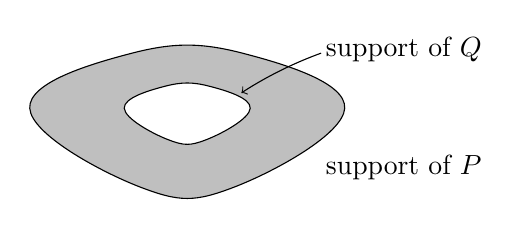
\begin{tikzpicture}
		\draw [fill=gray!50!white] plot [smooth cycle, tension=0.7] coordinates {(-2, 0) (-0.7, 0.7) (0.7, 0.7) (2, 0) (0.6, -1) (-0.6, -1) };
		
		\draw [fill=white] plot [smooth cycle, tension=0.7] coordinates {(-2/2.5, 0) (-0.7/2.5, 0.7/2.5) (0.7/2.5, 0.7/2.5) (2/2.5, 0/2.5) (0.6/2.5, -1/2.5) (-0.6/2.5, -1/2.5)};
		
		\draw [->] (1.7,0.7) arc(110:123:5);
		\node at (2.75,0.75) {support of $Q$};
		\node at (2.75, -0.75) {support of $P$};
	\end{tikzpicture}
\end{center}

\begin{prop}
	Let $P,Q$ have densities $p(x),q(x)$ with respect to a measure $\mu$
 on $\mathcal{X}$. Then the following are equivalent:
 \begin{enumerate}
 	\item $Q$ is absolutely continuous with respect to $P$.
 	\item $Q\left(\left\{x:\frac{p(x)}{q(x)} = 0\right\}\right) = 0$.
 	\item $\mathbb{E}_P\left[\frac{q(x)}{p(x)}\right] = 1$.
 \end{enumerate}
\end{prop}

\begin{proof}
	\quad
	\begin{enumerate}
		\item It is equivalent to: For $\mu$-a.e. $x \in \mathcal{X}$ where $p(x) = 0$, we must also have $q(x) = 0$.
		\item We rewrite the left hand side,
		\begin{equation*}
			Q\left(\left\{x: \frac{p(x)}{q(x)}\right\}\right) = \int \mathbbm{1}\{p(x) = 0\} \cdot q(x) \d \mu(x).
		\end{equation*} 
		This is $0$ if and only if (i) holds.
		\item We rewrite the left hand side,
		\begin{equation*}
			\begin{aligned}
				\mathbb{E}_P\left[\frac{q(x)}{p(x)}\right] &= \int \frac{q(x)}{p(x)} \cdot \mathbbm{1}\{p(x) > 0\} \cdot p(x) \d \mu (x) \\
				&= \int \mathbbm{1}\{p(x) > 0\} \cdot q(x) \d \mu (x) \\
				&= 1 - \int \mathbbm{1}\{p(x) = 0\} \cdot q(x) \d \mu(x) \\
				&= 1- Q\left(\left\{x: \frac{p(x)}{q(x)}\right\}\right).
			\end{aligned}
		\end{equation*}
		This is $1$ if and only if (ii) holds.
	\end{enumerate}
\end{proof}

\noindent For contiguity $Q_n \vartriangle P_n$, there is an ``asymptotic version" of the preceding result.

\begin{thm}[Le Cam's First Lemma]
	Let $P_n,Q_n$ be ($n$-indexed sequences of) probability distributions on $\mathcal{X}_n$, having densities $p_n$ and $q_n$ with respect to some common measure $\mu_n$. Suppose that,
	\begin{equation*}
		\begin{aligned}
			& \text{ Under } Q_n: \frac{p_n(x)}{q_n(x)} \stackrel{\text{d}}{\longrightarrow} U. \\
			& \text{ Under } P_n: \frac{q_n(x)}{p_n(x)} \stackrel{\text{d}}{\longrightarrow} V.
		\end{aligned}
	\end{equation*}
	Then the following are equivalent
	\begin{enumerate}
		\item $Q_n \vartriangle P_n$.
		\item $\mathbb{P}[U = 0] = 0$.
		\item $\mathbb{E}[V] = 1$.
	\end{enumerate}
\end{thm}

\begin{proof}[Partial proof]
	We'll show (ii) $\implies$ (i) and also (iii) $\implies$ (i). \\
	In both cases, suppose $E_n \subset \mathcal{X}_n$ satisfies $P_n(E_n) \equiv \alpha_n \to 0$. Write
	\begin{equation*}
		\begin{aligned}
			Q_n(E_n) &= Q_n \left(E_n \bigcap \left\{x: q_n(x) \leq t p_n(x)\right\}\right) + Q_n \left(E_n \bigcap \left\{x: q_n(x) > t p_n(x)\right\}\right) \\
			&\equiv \text{I} + \text{II} \quad \text{for a constant } t > 0.
		\end{aligned}
	\end{equation*}
	To bond I,
	\begin{equation*}
		\begin{aligned}
			\text{I} &= \int \mathbbm{1}\{x \in E_n\} \cdot \mathbbm{1}\{q_n(t) \leq tp_n(x)\} \cdot q_n(x) \d \mu_n (x) \\
			&\leq \int \mathbbm{1}\{x \in E_n\} \cdot tp_n(x) \d \mu_n (x) \\
			&= t \cdot P_n(E_n) \\
			&= t \cdot \alpha_n \to 0 \quad \text{ for any fixed } t > 0 \text{ as } n \to \infty.
		\end{aligned}
	\end{equation*}
	\newline
	It remains to bound II.
	\begin{itemize}
		\item To prove (ii) $\implies$ (i):
		\begin{equation*}
			\begin{aligned}
				\text{II} &\leq Q_n \left(\{q_n(x) > tp_n(x)\}\right) \\
				&= Q_n \left(\{x: \frac{p_n(x)}{q_n(x)} < \frac{1}{t}\}\right) \quad \text{(We may assume $q_n(x) > 0$ when $X \sim Q_n$)}.
			\end{aligned}
		\end{equation*}
		Let $U_n$ be a random variable with the distribution of $\frac{p_n(x)}{q_n(x)}$ when $X \sim Q_n$. The condition (ii) says $U_n \stackrel{\text{d}}{\longrightarrow} U$ where $\mathbb{P}[U = 0] = 0$. Fix any $\epsilon > 0$. Pick $t$ sufficiently large such that
		\begin{itemize}
			\item $\mathbb{P}\left[U < \frac{1}{t} < \epsilon\right]$.
			\item $\frac{1}{t}$ is a continuity point of the CDF of $U$.
		\end{itemize}
		Then
		\begin{equation*}
			\mathbb{P}\left[U_n < \frac{1}{t}\right] \to \mathbb{P}\left[U < \frac{1}{t}\right] < \epsilon.
		\end{equation*}
		So
		\begin{equation*}
			\sup \text{II} \leq \epsilon \text{ where } \epsilon \text{ is arbitary.} \implies \text{II} \to 0.
		\end{equation*}
		This shows $Q_n(E_n) \to 0$ (i.e., $Q_n \vartriangle P_n$).
		\item To prove (iii) $\implies$ (i):
		\begin{equation*}
			\begin{aligned}
				\text{II} &\leq Q_n \{x:q_n(x) > tp_n(x)\}) \\
				&= 1- Q_n(\{q_n(x) \leq tp_n(x)\}) \\
				&= 1- \int \mathbbm{1}\{q_n(x) \leq tp_n(x)\} \cdot q_n(x) \d \mu_n(x) \\
				&= 1- \int_{x:p_n(x) > 0} \mathbbm{1}\left\{\frac{q_n(x)}{p_n(x)} \leq t\right\} \cdot \frac{q_n(x)}{p_n(x)} \cdot p_n(x) \d \mu_n(x).
			\end{aligned}
		\end{equation*}
		Let $V_n$ be a random variable with the distribution of $\frac{q_n(x)}{p_n(x)}$ where $X \sim P_n$. Then the above is
		\begin{equation*}
			\text{II} \leq 1- \mathbb{E}\left[\mathbbm{1}\{V_n \leq t\} \cdot V_n \right].
		\end{equation*}
		The condition (iii) says $V_n \stackrel{\text{d}}{\longrightarrow} V$ where $\mathbb{E}[V] = 0$. Fix any $\epsilon > 0$. Pick $t$ sufficiently large such that
		\begin{itemize}
			\item $\mathbb{E}\left[\mathbbm{1}\{V \leq t\} \cdot V\right] > 1-\epsilon$.
			\item $t$ is a continuity point of the CDF of $V$.
		\end{itemize}
		\begin{claim}
			$\mathbb{E}\left[\mathbbm{1}\{V_n \leq t\} \cdot V_n\right] \to \mathbb{E}\left[\mathbbm{1}\{V \leq t\} \cdot V\right] > 1-\epsilon$
		\end{claim}
		\begin{proof}
			Let $f(x)$ be a continuous approximation of $\mathbbm{1}\{x \leq t\} \cdot x$:
			\begin{equation*}
				f(x) = \left\{ \begin{array}{ll}
					0 & x \leq 0 \\
					x & 0 < x \leq t \\
					\in (0,t) & t < x \leq t + \delta \\
					0 & x > t + \delta 
				\end{array}\right. \text{ for some } \delta > 0.
			\end{equation*}
			\begin{center}
				\begin{tikzpicture}
					\draw [->] [semithick] (-2, 0) -- (3.5, 0) node [right] {$x$};
					\draw [->] [semithick] (0, -1) -- (0, 1.5) node [above] {$f(x)$};
					
					\draw [mblue, thick, domain=-1.5:0] plot (\x, 0) node [] {};
					\draw [mblue, thick, domain= 0:1] plot (\x, \x) node [] {};
					\draw [mblue, thick, domain= 1:1.5] plot (\x, -2 * \x + 3) node [] {};
					\draw [mblue, thick, domain= 1.5:3] plot (\x,0) node [] {};
					
					\draw [dashed] (1,1) -- (1,0) node [below] {$t$};
					\draw [dashed] (1,1) -- (0,1) node [left] {$t$};
					\draw (1.5,0) -- (1.5,0) node [below] {$t+\delta$};
					\draw (1.75,0.5) -- (1.75,0.5) node [above] {$f(x)$};
				\end{tikzpicture}
			\end{center}
			Since $f$ is continuous and bounded and $V_n \stackrel{\text{d}}{\longrightarrow} V$, we have
			\begin{equation*}
				\mathbb{E}[f(V_n)] \to \mathbb{E}[f(V)].
			\end{equation*}
			On the other hand,
			\begin{equation*}
				\begin{aligned}
					\mathbb{E}[f(V_n)] &\geq \mathbb{E}\left[\mathbbm{1}\{V_n \leq t\} \cdot V_n\right] \\
					&\geq \mathbb{E}\left[f(V_n)\right] - t \cdot \mathbb{P} \left[V_n \in (t,t+\delta)\right] \quad \text{(Since $V_n \geq 0$)}.
				\end{aligned}
			\end{equation*}
			Take $\delta$ such that $t+\delta$ is also a continuity point of the CDF of $V$. Then
			\begin{equation*}
				\mathbb{P}[V_n \in (t,t+\delta)] \to \mathbb{P}[V \in (t,t+\delta)]
			\end{equation*}
			Then
			\begin{equation*}
				\begin{aligned}
					\mathbb{E}[f(V)] &\geq \lim\limits_{n \to \infty} \sup \mathbb{E}\left[\mathbbm{1}\{V_n \leq t\} \cdot V_n\right] \\
					&\geq \lim\limits_{n \to \infty} \inf \mathbb{E}\left[\mathbbm{1}\{V_n \leq t\} \cdot V_n\right] \\
					&\geq \mathbb{E}\left[f(V_n)\right] - t \cdot \mathbb{P} \left[V_n \in (t,t+\delta)\right].
				\end{aligned}
			\end{equation*}
			Since $\delta$ is arbitrarily small, this yields
			\begin{equation*}
				\mathbb{E}\left[\mathbbm{1}\{V_n \leq t\} \cdot V_n\right] \to \mathbb{E}\left[\mathbbm{1}\{V \leq t\} \cdot V\right] > 1 - \epsilon.
			\end{equation*}
		\end{proof}
		By Claim 6.1.1, 
		\begin{equation*}
			\sup \text{II} \leq 1- (1-\epsilon) = \epsilon \text{ where } \epsilon \text{ is arbitary.} \implies \text{II} \to 0.
		\end{equation*}
		This shows $Q_n(E_n) \to 0$ (i.e., $Q \vartriangle P$).
	\end{itemize}
	To prove (i) $\implies$ (ii) and (i) $\implies$ (iii), see \emph{Theory of Point Estimation} Theorem 12.3.2, \emph{van der Vaart} Lemma 6.4.
\end{proof}

\begin{note}
	If $\frac{q_n(x)}{p_n(x)} \stackrel{\text{d}}{\longrightarrow} V$ under $P_n$, $\mathbb{P}[V = 0] = 0$, $\mathbb{E}[V] = 1$, then $Q_n \vartriangleleft \vartriangleright P_n$. 
\end{note}

\begin{remark}
	Actually, we don't need to assume $\frac{p_n(x)}{q_n(x)} \stackrel{\text{d}}{\longrightarrow} U$ under $Q_n$ and $\frac{q_n(x)}{p_n(x)} \stackrel{\text{d}}{\longleftrightarrow} V$ under $P_n$. If $\frac{p_n(x)}{q_n(x)} \stackrel{\text{d}}{\longrightarrow} U$ along any subsequence, or $\frac{q_n(x)}{p_n(x)} \stackrel{\text{d}}{\longrightarrow} V$ along any subsequence, then the preceding still shows $Q_n \vartriangle P_n$. See \emph{van der Vaart} Theorem 6.4 for a full statement.
\end{remark}

\begin{eg}
	Consider $\mathcal{X}_n = \mathbb{R}^n$.
	\begin{itemize}
		\item $P_n = \text{joint law of } X_1,X_2,\cdots,X_n \stackrel{\text{i.i.d.}}{\sim} n(\theta_0,\sigma^2)$.
		\item $Q_n = \text{joint law of } X_1,X_2,\cdots,X_n \stackrel{\text{i.i.d.}}{\sim} N(\theta_1,\sigma^2)$  where $\theta_1 \equiv \theta_0+\frac{h}{\sqrt{n}}$ for a fixed local parameter $h > 0$.
	\end{itemize}
	We are going to show $Q_n \vartriangleleft \vartriangleright P_n$.
	\begin{equation*}
		\begin{aligned}
			\frac{q_n(x)}{p_n(x)} &= \exp \left(\frac{n(\theta_1-\theta_0)}{\sigma^2} \cdot \bar{x} - \frac{n(\theta_1^2-\theta_0^2)}{2\sigma^2}\right) \\
			&= \exp \left(\frac{h}{\sigma^2} \cdot \sqrt{n} \bar{x} - \frac{h}{\sigma^2} \cdot \sqrt{n} \theta_0 - \frac{h^2}{2\sigma^2}\right) \\
			&= \exp \left(\frac{h}{\sigma^2} \cdot \sqrt{n} (\bar{x} - \theta_0) - \frac{h^2}{2\sigma^2}\right).
		\end{aligned}
	\end{equation*}
	Under $P_n$, we have
	\begin{equation*}
		\frac{q_n(x)}{p_n(x)} \stackrel{\text{L}}{=} e^W \quad \text{where $W \sim N(-\frac{h^2}{2\sigma^2},\frac{h^2}{\sigma^2})$.}
	\end{equation*}
	\emph{The mean of $W$ is $-\frac{1}{2}$ times the variance}. \\
	Note: For any $Z \sim N(\mu,\sigma^2)$, $\mathbb{E}\left[e^Z\right] = e^{\mu + \frac{1}{2} \sigma^2}$. So
	\begin{equation*}
		\begin{aligned}
			& \mathbb{E}\left[e^W\right] = 1 \implies \text{By Le Cam’s First Lemma ((iii) $\implies$ (i))}, \ Q_n \vartriangle P_n. \\
			& \mathbb{P}\left[e^W = 0\right] = 0 \implies \text{By Le Cam’s First Lemma ((ii) $\implies$ (i))}, \ P_n \vartriangle Q_n.
		\end{aligned}
	\end{equation*}
	So $P_n \vartriangleleft \vartriangleright Q_n$.
\end{eg}

\begin{cor}
	Suppose $P_n,Q_n$ are such that $\log \frac{q_n(x)}{p_n(x)} \to W$ under $P_n$, where $W \sim N(\mu,\sigma^2)$. Then $P_n \vartriangle Q_n$ always, and $Q_n \vartriangle P_n$ if and only if $\mu = -\frac{1}{2} \sigma^2$.
\end{cor}

\subsection{Local Asymptotic Normality}

\textbf{Setup:}. Consider $X_1,X_2,\cdots,X_n \stackrel{\text{i.i.d.}}{\sim} p_\theta$, $\theta \in \Omega \subseteq \mathbb{R}^k$. Let $\theta_0$ be in the interior of $\Omega$. Our goal is to show under mild conditions, $P_n: X_1,X_2,\cdots,X_n \stackrel{\text{i.i.d.}}{\sim} p_{\theta_0}$ and $Q_n: X_1,X_2,\cdots,X_n \stackrel{\text{i.i.d.}}{\sim} P_{\theta_0+\frac{h}{\sqrt{n}}}$ are mutually contiguous. \\

\noindent \textbf{Heuristic calculation:} Write $l(\theta|x) = \sum\limits_{i=1}^n l(\theta|x_i) = \sum\limits_{i=1}^n \log p_{\theta}(x_i)$. Applying a Taylor expansion, we expect for fixed $h \in \mathbb{R}^k$
\begin{equation*}
	\begin{aligned}
		\log L_{n,h} \equiv \log \frac{\prod\limits_{i=1}^n p_{\theta_0 + \frac{h}{\sqrt{n}}} (x_i)}{\prod\limits_{i=1}^n p_{\theta_0} (x_i)} &= l(\theta_0 + \frac{h}{\sqrt{n}} | x) - l(\theta_0 | x) \\
		&\approx \frac{h}{\sqrt{n}}^T \cdot \nabla l(\theta_0|x) + \frac{1}{2} \frac{h}{\sqrt{n}}^T \cdot \nabla^2 l(\theta_0 |x) \cdot \frac{h}{\sqrt{n}} \\
		&= \left[\frac{1}{\sqrt{n}} \nabla l(\theta_0|x) \right]^T h - \frac{1}{2}h^T \left[-\frac{1}{n}\nabla^2 l(\theta_0 | \ x)\right] h.
	\end{aligned}
\end{equation*}
Under $\theta_0$:
\begin{itemize}
	\item[$\circ$] $\frac{1}{\sqrt{n}} \nabla l(\theta_0|x) \stackrel{\text{d}}{\longrightarrow} N(0,I(\theta_0))$.
	\item[$\circ$] $-\frac{1}{n}\nabla^2l(\theta_0|x) \stackrel{\text{P}}{\longrightarrow} I(\theta_0)$.
\end{itemize}
So we expect 
\begin{equation*}
	\begin{aligned}
		& \log L_{n,h} \stackrel{\text{d}}{\longrightarrow} N\left(-\frac{1}{2}h^TI(\theta_0)h,h^TI(\theta_0)h\right). \\
		& L_{n,h} \stackrel{\text{d}}{\longrightarrow} e^W \text{ where } W \sim N\left(-\frac{1}{2}h^TI(\theta_0)h,h^TI(\theta_0)h\right)
	\end{aligned}
\end{equation*}
Then by Le Cam’s First Lemma,
\begin{equation*}
	\left. \begin{array}{l}
		\circ \quad \mathbb{P} \left[e^w = 0\right] = 0 \vspace{1ex} \\
		\circ \quad \mathbb{E} \left[e^W\right] = 1
	\end{array} \right\} \implies Q_n \vartriangleleft \vartriangleright P_n.
\end{equation*}

\noindent \textbf{To make this rigorous:} \\
The following weak regularity condition is all that's needed.

\begin{defi}[Quadratic mean differentiable]\index{quadratic mean differentiable}
	Let $\{P_\theta: \theta \in \Omega\}$ have densties $p_{\theta}$ with respect to a common measure $\mu$. Let $\theta_0 \in \Omega \subseteq \mathbb{R}^k$ be an interior point. This model is \emph{quadratic mean differentiable} (q.m.d.) at $\theta_0$ if there is a function $\dot{l}: \mathcal{X} \to \mathbb{R}^k$ such that
	\begin{equation}
		\frac{1}{\Vert t \Vert^2} \int_{\mathcal{X}} \left(\sqrt{p_{\theta_0+t}(x)} - \sqrt{p_{\theta_0}(x)} - \frac{1}{2} \sqrt{p_{\theta_0}(x)} \dot{l}(x)^T t\right)^2 \d \mu (x) \to 0 \text{ as } t \to 0.
	\end{equation}
\end{defi}

\noindent \textbf{Interpretation:} Suppose $\theta \to \sqrt{p_{\theta}(x)}$ is differentiable. By Taylor expansion,
\begin{equation*}
	\sqrt{p_{\theta+t}(x)} = \sqrt{p_{\theta}(x)} + \frac{1}{2\sqrt{p_{\theta}(x)}} \nabla p_{\theta}(x)^T t + O(t^2).
\end{equation*}
We should identify 
\begin{equation*}
	\frac{1}{2\sqrt{p_{\theta}(x)}} \nabla p_{\theta}(x)^T t = \frac{1}{2} \sqrt{p_{\theta_0}(x)} \dot{l}(x)^T t. 
\end{equation*}
Then
\begin{equation*}
	\dot{l} (x) = \frac{\nabla p_{\theta}(x)}{p_\theta(x)} = \nabla \log p_{\theta}(x).
\end{equation*}
In this context, $\dot{l}(x)$ is the simple-sample score. The usual score is $Z_n = \frac{1}{\sqrt{n}} \sum\limits_{i=1}^n \dot{l} (x_i)$ and the Fisher information is $I(\theta_0) = \mathbb{E}_{\theta_0} \left[\dot{l}(X_i) \dot{l}(X_i)^T \right]$.

\begin{prop}[Sufficient condition for q.m.d.]
	If $\theta \to \sqrt{p_{\theta}(x)}$ is continuously differentiable in $\theta$ for $\mu$-a.e. $x$, and the entries of $I(\theta) = \mathbb{E}\left[\nabla l(\theta|X_i) \nabla l(\theta|X_i)^T \right]$
	are well-defined and continuous in $\theta$, then the model is q.m.d. with
	\begin{equation*}
		\frac{1}{2} \sqrt{p_{\theta_0}(x)} \dot{l} (x) = \nabla \sqrt{p_{\theta}(x)} \big| _{\theta = \theta_0}.
	\end{equation*}
	So
	\begin{equation*}
		\dot{l} (x) = \nabla \log p_{\theta} (x) \big|_{\theta = \theta_0} = \frac{\nabla p_{\theta} (x) \big|_{\theta = \theta_0}}{p_{\theta_0}(x)}.
	\end{equation*}
\end{prop}

\begin{proof}
	See \emph{van der Vaart} Lemma 7.6.
\end{proof}

\begin{note}
	q.m.d. holds for
	\begin{itemize}
		\item Exponential families.
		\item Location models $p_{\theta}(x) = f(x-\theta)$ where $\theta \in \mathbb{R}$, $f: \mathbb{R}^k \to \mathbb{R}$ is a fixed function such that $\sqrt{f}$ is absolutely continuous and $I \equiv \int \frac{f'(x)^2}{f(x)} \d x < \infty$. In particular: $Cauchy(\theta,1),Laplace(\theta,1)$. 
	\end{itemize}
\end{note}

\begin{thm}[Local Asymptotic Normality]
	Suppose $\{P_{\theta}: \theta \in \Omega\}$ is q.m.d. at $\theta_0 \in \Omega \subseteq \mathbb{R}^k$. Define the score $Z_n = \frac{1}{\sqrt{n}} \sum\limits_{i=1}^n \dot{l} (x_i)$, and the Fisher information $I(\theta_0) = \mathbb{E}_{\theta_0} \left[\dot{l}(X_i) \dot{l}(X_i)^T\right]$. Then for each fixed $h \in \mathbb{R}^k$, as $n \to \infty$,
	\begin{enumerate}
		\item $\log L_{n,h} \equiv \log \frac{\prod\limits_{i=1}^n p_{\theta_0 + \frac{h}{\sqrt{n}}} (x_i)}{\prod\limits_{i=1}^n p_{\theta_0} (x_i)} = Z_n^T h - \frac{1}{2} h^T I(\theta_0) h + r_n$, where $r_n \stackrel{\text{P}}{\longrightarrow} 0$ under $\theta_0$.
		\item Therefore, under $\theta_0$, $L_{n,h} \stackrel{\text{d}}{\longrightarrow} e^W$, $W \sim N(-\frac{1}{2}h^TI(\theta_0)h,h^TI(\theta_0)h)$.
	\end{enumerate}
\end{thm}

\begin{cor}
		By Le Cam's First Lemma, $P_{\theta_{\theta_0+\frac{h}{\sqrt{n}}}}^n \vartriangleleft \vartriangleright P_{\theta_0}^n$. 
\end{cor}

\begin{proof}
	Fix $h \in \mathbb{R}^k$. Write as shorthand $p(x) \equiv p_{\theta_0}(x), p_n(x) \equiv p_{\theta_0 + \frac{h}{\sqrt{n}}} (x)$.
	\begin{itemize}[leftmargin=*]
		\item Step 0: $\mathbb{E}_{\theta_0} \left[Z_n^T h\right] = 0, \ h^TI(\theta_0)h < \infty$.
		\begin{proof}
			Write $\left\langle f,g \right\rangle_{\mu} = \int f(x)g(x) \d \mu (x), \ \Vert f \Vert^2_{\mu} = \left\langle f,f \right\rangle_{\mu} = \int f(x)^2 \d \mu (x)$. Apply q.m.d. condition with $t = \frac{h}{\sqrt{n}}$,
			\begin{equation*}
				\frac{n}{\Vert h \Vert^2} \left\Vert \sqrt{p_n} - \sqrt{p} - \frac{1}{2} \sqrt{p} \ \dot{l}^T \frac{h}{\sqrt{n}}\right\Vert_{\mu}^2 \to 0.
			\end{equation*}
			So
			\begin{equation*}
				\left\Vert \sqrt{n} \left(\sqrt{p_n} - \sqrt{p}\right) - \frac{1}{2} \sqrt{p} \ \dot{l}^T \frac{h}{\sqrt{n}}\right\Vert_{\mu}^2 \to 0.
			\end{equation*}
			\begin{itemize}
				\item To prove $h^T I(\theta_0) h < \infty$,
				\begin{equation*}
					\begin{aligned}
						h^T I(\theta_0) h &= \mathbb{E}_{\theta_0} \left[h^T \dot{l}(X_i) \dot{l}(X_i)^T h\right] \\
						&= \mathbb{E}_{\theta_0} \left[ \left(\dot{l}(X_i)^T h\right)^2 \right] \\
						&= \int \left(\dot{l}(x_i)^T h\right)^2 p(x_i) \d \mu (x) \\
						&= \left\Vert \sqrt{p} \ \dot{l}^T h\right\Vert_{\mu}^2.
					\end{aligned}
				\end{equation*}
				Since
				\begin{equation*}
					\begin{aligned}
						\left\Vert \sqrt{p} \ \dot{l}^T h\right\Vert_{\mu} &\leq 2 \cdot \left\Vert \sqrt{n} \left(\sqrt{p_n} - \sqrt{p}\right) \right\Vert_{\mu} + 2 \cdot \left\Vert \frac{1}{2}\sqrt{p} \ \dot{l}^T h -\sqrt{n} \left(\sqrt{p_n} - \sqrt{p}\right)\right\Vert \\
						&\leq 2 \cdot \Vert \sqrt{n} \sqrt{p_n} \Vert_{\mu} + 2 \cdot \Vert \sqrt{n} \sqrt{p} \Vert_{\mu} + 2 \cdot \left\Vert \frac{1}{2}\sqrt{p} \ \dot{l}^T h -\sqrt{n} \left(\sqrt{p_n} - \sqrt{p}\right)\right\Vert \\
						&\equiv 2 \cdot \Vert \sqrt{n} \sqrt{p_n} \Vert_{\mu} + 2 \cdot \Vert \sqrt{n} \sqrt{p} \Vert_{\mu} + 2 \epsilon_n \text{ where $\epsilon_n \to 0$ by q.m.d.} \\
						&= 2 \cdot \left(\int n \cdot p_n \ \d \mu \right)^\frac{1}{2} + 2 \cdot \left(\int n \cdot p \ \d \mu \right)^\frac{1}{2} + 2 \epsilon_n \\
						&= 4 \cdot \sqrt{n} + 2 \epsilon_n.
					\end{aligned}
				\end{equation*}
				Since $\sqrt{p} \ \dot{l}^T h$ is independent of $n$, this implies $\Vert \sqrt{p} \ \dot{l}^T h\Vert_{\mu} < \infty$. Then $h^TI(\theta_0)h < \infty$.
				\item To prove $\mathbb{E}_{\theta_0} \left[l(X_i)^T h\right]$, we first consider
				\begin{equation*}
					\mathbb{E}_{\theta_0} \left[\dot{l} (X_i)^T h\right] = \int \left(\dot{l} (x_i) p(x) \right) \d \mu(x) = \left \langle \frac{1}{2} \sqrt{p} \ \dot{l}^T h, 2\sqrt{p} \right \rangle_{\mu}.
				\end{equation*}
				Note:
				\begin{equation*}
					\begin{aligned}
						&\Vert 2\sqrt{p} - \left(\sqrt{p} + \sqrt{p_n}\right)\Vert_{\mu} = \Vert \sqrt{p} - \sqrt{p_n} \Vert_{\mu} \\
						&= \frac{1}{\sqrt{n}} \left\Vert \frac{1}{2}\sqrt{p} \ \dot{l}^T h  \right\Vert_{\mu} +  \frac{1}{\sqrt{n}} \left \Vert \sqrt{n} \left(\sqrt{p_n} - \sqrt{p}\right) - \frac{1}{2}\sqrt{p} \ \dot{l}^T h \right \Vert_{\mu} \to 0.
					\end{aligned}
				\end{equation*}
				By q.m.d. and $\sqrt{p} \ \dot{l}^T h$ is independent of $n$, $\Vert 2\sqrt{p} - \left(\sqrt{p} + \sqrt{p_n}\right)\Vert_{\mu} \to 0$.
				Then
				\begin{equation*}
					\begin{aligned}
						\mathbb{E}_{\theta_0} \left[\dot{l} (X_i)^T h\right] &= \left \langle \frac{1}{2} \sqrt{p} \ \dot{l}^T h, 2\sqrt{p} \right \rangle_{\mu} \\
						&= \lim\limits_{n \to \infty} \left \langle \sqrt{n}(\sqrt{p_n}-\sqrt{p}), \sqrt{p} + \sqrt{p_n} \right \rangle_{\mu} \\
						&= \int \sqrt{n}(\sqrt{p_n}-\sqrt{p}) (\sqrt{p} + \sqrt{p_n}) \d \mu\\
						&= \int \sqrt{n}(p_n-p) \d \mu = 0.
					\end{aligned}
				\end{equation*}
				So this shows $\mathbb{E}_{\theta_0} \left[\dot{l} (X_i)^T h\right] = 0$, also $\mathbb{E}_{\theta_0} \left[Z_n^T h\right] = 0$.
			\end{itemize}
		\end{proof}
		\item Step 1: Split $\log L_{n,h} \equiv \log \frac{\prod\limits_{i=1}^n p_{\theta_0 + \frac{h}{\sqrt{n}}} (x_i)}{\prod\limits_{i=1}^n p_{\theta_0} (x_i)} = 2 \sum\limits_{i=1}^n \log \sqrt{\frac{p_n(x_i)}{p(x_i)}}$.\\
		Let $W_n(x_i) = 2 \left(\sqrt{\frac{p_n(x_i)}{p(x_i)}} -1\right)$, then apply Taylor expansion
		\begin{equation*}
			\log (1+x) = x - \frac{x^2}{2} + x^2 R(x) \text{ where $R(x) \to 0$ as $x \to 0$}.
		\end{equation*}
		Then
		\begin{equation*}
			\begin{aligned}
				\log L_{n,h} &= 2 \cdot \sum\limits_{i=1}^n \log \left(1 + \frac{1}{2} W_n(x_i)\right) \\
				&= 2 \cdot \left( \sum\limits_{i=1}^n \left(\frac{1}{2} W_n(x_i) - \frac{1}{8} W_n(x_i)^2 +  \frac{1}{4} W_n(x_i)^2 \cdot R \left(\frac{1}{2} W_n(x_i)\right)\right) \right) \\
				&= \sum\limits_{i=1}^n W_n(x_i) - \frac{1}{4} \cdot \sum\limits_{i=1}^n W_n(x_i)^2 + \frac{1}{2} \cdot \sum\limits_{i=1}^n W_n(x_i)^2 \cdot R\left(\frac{1}{2} W_n(x_i)\right).
			\end{aligned}
		\end{equation*}
		\item Step 2: $\sum\limits_{i=1}^n W_n(x_i) = Z_n^Th - \frac{1}{4} \cdot h^T I(\theta_0) h + r_n$ where $r_n \stackrel{\text{P}}{\longrightarrow} 0$ under $\theta_0$.
		\begin{proof}
			Define $r_n = \sum\limits_{i=1}^n W_n(x_i) - Z_n^Th + \frac{1}{4} \cdot h^T I(\theta_0) h$.
			\begin{itemize}
				\item To prove $\mathbb{E}_{\theta_0}[r_n] \to 0$,
				\begin{equation*}
					\begin{aligned}
						\mathbb{E}_{\theta_0} \left[\sum\limits_{i=1}^n W_n(X_i)\right] &= n \cdot \mathbb{E}_{\theta_0} \left[W_n(X_i)\right] \\
						&= n \cdot \int 2 \left(\sqrt{\frac{p_n(x_i)}{p(x_i)}} -1\right) \cdot p \ \d \mu \\
						&= n \left(\int 2\sqrt{p_n \cdot p} \ \d \mu -2\right) \\
						&= n \cdot \left(\int 2\sqrt{p_n \cdot p} \ \d \mu - \int p_n \ \d \mu - \int p \ \d \mu\right) \\
						&= -n \cdot \left(\int (\sqrt{p_n} - \sqrt{p})^2 \ \d \mu\right) \\
						&= -\Vert \sqrt{n} (\sqrt{p_n}-\sqrt{p}) \Vert_{\mu}^2 \\
						&\to -\left\Vert \frac{1}{2} \sqrt{p} \ \dot{l}^T h \right\Vert_{\mu}^2 \\
						&= -\frac{1}{4} \int \left(\dot{l}^Th\right)^2 \cdot p \ \d \mu \\
						&= -\frac{1}{4} \mathbb{E}_{\theta_0} \left[\left(\dot{l}^Th\right)^2 \right] = -\frac{1}{4} h^T I(\theta_0) h.
					\end{aligned}
				\end{equation*}
				Since $E_{\theta_0} \left[Z_n^T h\right] = 0$, we have $\mathbb{E}_{\theta_0}[r_n] \to 0$.
				\item To prove $Var_{\theta_0}(r_n) \to 0$.
				\begin{equation*}
					\begin{aligned}
						Var_{\theta_0}[r_n] &= Var_{\theta_0} \left[\sum\limits_{i=1}^n W_n(x_i) - Z_n^Th\right] \\
						&= Var_{\theta_0} \left[\sum\limits_{i=1}^n \left(W_n(X_i) - \frac{1}{\sqrt{n}} \dot{l}(X_i)^T h \right)\right] \\
						&= n \cdot Var_{\theta_0} \left[\left(W_n(X_i) - \frac{1}{\sqrt{n}} \dot{l}(X_i)^T h \right)\right] \\
						&\leq n \mathbb{E}_{\theta_0} \left[\left(W_n(X_i) - \frac{1}{\sqrt{n}} \dot{l}(X_i)^T h\right)^2\right] \\
						&= n \dot \int \left(2\left(\frac{p_n}{p}\right)-\frac{1}{\sqrt{n}} \ \dot{l}^T h\right)^2 \cdot p \ \d \mu. \\
						&= 4 \cdot \int \left(\sqrt{n}(\sqrt{p_n} - \sqrt{p})- \frac{1}{2} \sqrt{p} \ \dot{l}^T h \right)^2 \d \mu \\
						&= 4 \cdot \left\Vert \sqrt{n}(\sqrt{p_n} - \sqrt{p})- \frac{1}{2} \sqrt{p} \ \dot{l}^T h \right\Vert_{\mu}^2 \to 0.
					\end{aligned}
				\end{equation*}
			\end{itemize}
			So $r_n \stackrel{\text{P}}{\longrightarrow} 0$.
		\end{proof}
		\item Step 3: $\sum\limits_{i=1}^n W_n(x_i)^2 \stackrel{\text{P}}{\longrightarrow}h^T I(\theta_0) h$ under $\theta_0$.
		\begin{proof}
			Define $A_n(x_i) = W_n(x_i) - \frac{1}{\sqrt{n}} \ \dot{l} (x_i)^T h$. By the variance computation of Step 2, we have $n \cdot \mathbb{E}_{\theta_0} \left[A_n(x_i)^2\right] \to 0$ under $\theta_0$ $(\ast)$. Write
			\begin{equation*}
				\begin{aligned}
					W_n(x_i)^2 &= \left(A_n(x_i) + \frac{1}{\sqrt{n}} \ \dot{l} (x_i)^T h\right)^2 \\
					&= \frac{1}{n} \left(\dot{l} (x_i)^T h\right)^2 + \frac{2}{\sqrt{n}} \dot{l}(x_i)^T h \cdot A_n(x_i) + A_n(x_i)^2.
				\end{aligned}
			\end{equation*}
			Then
			\begin{equation*}
				\sum\limits_{i=1}^n W_n(x_i)^2 = \sum\limits_{i=1}^n \frac{1}{n} \left(\dot{l} (x_i)^T h\right)^2 + \sum\limits_{i=1}^n A_n(x_i)^2 + 2 \cdot \sum\limits_{i=1}^n \frac{1}{\sqrt{n}} \dot{l}(x_i)^T h \cdot A_n(x_i).
			\end{equation*}
			Since
			\begin{itemize}
				\item $\sum\limits_{i=1}^n \frac{1}{n} \left(\dot{l} (x_i)^T h\right)^2 \stackrel{\text{P}}{\longrightarrow} h^T I(\theta_0) h$ by Weak Law of Large Numbers.
				\item $\sum\limits_{i=1}^n A_n(x_i)^2 \stackrel{\text{P}}{\longrightarrow} 0$ by $(\ast)$ and Markov's Inequality.
				\item $ \sum\limits_{i=1}^n \frac{1}{\sqrt{n}} \dot{l}(x_i)^T h \cdot A_n(x_i) \stackrel{\text{P}}{\longrightarrow} 0$ by Cauchy–Schwarz Inequality.
			\end{itemize}
			We conclude that $\sum\limits_{i=1}^n W_n(x_i)^2 \stackrel{\text{P}}{\longrightarrow}h^T I(\theta_0) h$.
		\end{proof}
		\item Step 4: $\sum\limits_{i=1}^n W_n(x_i)^2 \cdot R\left(\frac{1}{2} W_n(x_i) \right) \stackrel{\text{P}}{\longrightarrow} 0$.
		\begin{proof}
			\begin{equation*}
				\sum\limits_{i=1}^n W_n(x_i)^2 \cdot R\left(\frac{1}{2} W_n(x_i) \right) \leq \sum\limits_{i=1}^n W_n(x_i)^2 \cdot \max\limits_{i=1}^n \abs{R\left(\frac{1}{2} W_n(x_i) \right)}
			\end{equation*}
			By Step 3, $\sum\limits_{i=1}^n W_n(x_i)^2 \stackrel{\text{P}}{\longrightarrow}h^T I(\theta_0) h$. So by continuous mapping, it suffices to show $ \max\limits_{i=1}^n \abs{W_n(x_i)} \stackrel{\text{P}}{\longrightarrow} 0$ to show $R\left(\frac{1}{2} W_n(x_i) \right) \stackrel{\text{P}}{\longrightarrow} 0$. \\
			\newline
			If we apply
			\begin{equation*}
				W_n(x_i)^2 = \left(\frac{1}{\sqrt{n}} \ \dot{l}(x_i)^T h + A_n(x_i)\right)^2 \leq \frac{2}{n} \cdot \left(\dot{l}(x_i)^T h\right)^2 + 2 \cdot A_n(x_i)^2.
			\end{equation*}
			Then
			\begin{equation*}
				\begin{aligned}
					\mathbb{P}_{\theta_0} \left[\max\limits_{i=1}^n \abs{W_n(x_i)} \geq \epsilon\right] &\leq n \cdot \mathbb{P}_{\theta_0} \left[W_n(x_i)^2 \geq \epsilon^2 \right] \\
					&\leq n \left(\mathbb{P}_{\theta_0} \left[\frac{1}{n} \cdot \left(\dot{l}(x_i)^T h\right)^2 \geq \frac{\epsilon^2}{4} \right] + \mathbb{P}_{\theta_0} \left[A_n(x_i)^2 \geq \frac{\epsilon^2}{4} \right]\right).
				\end{aligned}
			\end{equation*}
			Note: For any random variable $Y \geq 0$, let $Z = Y \cdot \mathbbm{1}\{Y \geq t\}$,
			\begin{equation}
				\mathbb{P}[Y \geq t] = \mathbb{P}[Z \geq t] \leq \frac{1}{t} \cdot \mathbb{E}[Z] = \frac{1}{t} \cdot \mathbb{E}\left[Y \cdot \mathbbm{1}\{Y \geq t\}\right].
			\end{equation}
			Then
			\begin{itemize}
				\item $n \cdot \mathbb{P}_{\theta_0} \left[A(x_i)^2 \geq \frac{\epsilon^2}{4} \right] \leq \frac{4n}{\epsilon^2} \cdot \mathbb{E}_{\theta_0} \left[A(x_i)^2\right] \to 0$ by Markov's Inequality.
				\item $n \cdot \mathbb{P}_{\theta_0} \left[\frac{1}{n} \cdot \left(\dot{l}(x_i)^T h\right)^2 \geq \frac{\epsilon^2}{4} \right] \leq n \cdot \frac{4}{n\epsilon^2} \mathbb{E}_{\theta_0} \left[ \left(\dot{l}(x_i)^T h\right)^2 \cdot \mathbbm{1}\left\{\dot{l}(x_i)^T h \geq \frac{n\epsilon^2}{4}\right\}^2 \right]$ by (6.2.2). Since $\mathbb{E}_{\theta_0} \left[\left(\dot{l}(x_i)^T h\right)^2\right] = h^T I(\theta_0)h < \infty$, this $\to 0$ as $n \to \infty$ by Dominated Convergence Theorem.
			\end{itemize}
			This shows $\max\limits_{i=1}^n \abs{W_n(x_i)} \stackrel{\text{P}}{\longrightarrow} 0$ and then $\sum\limits_{i=1}^n W_n(x_i)^2 \cdot R\left(\frac{1}{2} W_n(x_i) \right) \stackrel{\text{P}}{\longrightarrow} 0$.
		\end{proof}
		\item Combining Step 1 - 4:
		\begin{equation}
			\begin{aligned}
				\log L_{n,h} &= Z_n^Th - \frac{1}{4} h^T I(\theta_0) h - \frac{1}{4} h^T I(\theta_0) h + r_n \\
				&= Z_n^Th - \frac{1}{2} h^T I(\theta_0) h + r_n \text{ where $r_n \stackrel{\text{P}}{\longrightarrow} 0$ under $\theta_0$}
			\end{aligned}
		\end{equation}
		This shows (i) in Theorem 6.2.1. Under $\theta_0$,
		\begin{equation}
			\begin{aligned}
				& Z_n^T h \stackrel{\text{d}}{\longrightarrow} N\left(0,h^TI(\theta_0)h\right) \quad \text{by Central Limit Theorem.} \\
				& \log L_{n,h} \stackrel{\text{d}}{\longrightarrow} N\left(- \frac{1}{2} h^T I(\theta_0) h, h^T I(\theta_0) h\right).
			\end{aligned}
		\end{equation}
		This shows (ii) in Theorem 6.2.1.
	\end{itemize}
\end{proof}

\subsection{Local Alternatives, Aymptotic Power}

\begin{eg}[Neyman-Pearon test]
	Suppose $X_1,X_2,\cdots,X_n \stackrel{\text{i.i.d.}}{\sim} p_{\theta}$, $\theta \in \mathbb{R}^k$. Assume the model is q.m.d. at $\theta_0$. Test
	\begin{equation*}
		H_0: \theta = \theta_0 \text{ v.s. } H_1: \theta = \theta_0 + \frac{h}{\sqrt{n}} \text{ for fixed $h \in \mathbb{R}^k$}.
	\end{equation*}
	By Neyman-Pearson Lemma, the most powerful test rejects $H_0$ when
	\begin{equation*}
		\log L_{n,h} \equiv \log \prod_{i=1}^n \frac{p_{\theta_0 + \frac{h}{\sqrt{n}}}(x_i)}{p_{\theta_0}(x_i)} > l_{n,h}^{(1-\alpha)}
	\end{equation*}
	where $l_{n,h}^{(1-\alpha)}$ is the $(1-\alpha)$-quantile of the distribution of $\log L_{n,h}$ under $H_0$.\\
	By Theorem 6.2.1., under $H_0: \theta = \theta_0$
	\begin{equation*}
		\log L_{n,h} \stackrel{\text{d}}{\longrightarrow} N\left(- \frac{1}{2} h^T I(\theta_0) h, h^T I(\theta_0) h\right) \equiv N\left(- \frac{1}{2} \sigma_h^2, \sigma_h^2\right).
	\end{equation*}
	Then $l_{n,h}^{(1-\alpha)}$ converges to the $(1-\alpha)$-quantile of this normal limit,
	\begin{equation*}
		l_{n,h}^{(1-\alpha)} \to - \frac{1}{2} \sigma_h^2 + \sigma_h \cdot z^{(1-\alpha)}.
	\end{equation*}
	\begin{question}
		What is the asymptotic power of this test?
	\end{question}
	\begin{answer}
		To compute the asymptotic power, we need to understand the distribution of $L_{n,h}$ not under $H_0$, but under $H_1$.
	\end{answer}

	\noindent \textbf{Heuristic calculation:} Let $p_n(l)$ be the density of $\log L_{n,h}(x)$ under $H_0$, and $p(l)$ be the density of its limit $N\left(- \frac{1}{2} \sigma_h^2, \sigma_h^2\right)$. Assuming $p_{\theta_0+\frac{h}{\sqrt{n}}}$ and $p_{\theta_0}$ have common support, we have for any function $f: \mathcal{X}^n \to \mathbb{R}$
	\begin{equation*}
		\begin{aligned}
			\mathbb{E}_{\theta_0+\frac{h}{\sqrt{n}}} \left[f(X_1,X_2,\cdots,X_n)\right] &= \int f(x_1,x_2,\cdots,x_n) \cdot \prod\limits_{i=1}^np_{\theta_0+\frac{h}{\sqrt{n}}} (x_i) \d x_i \\
			&= \int f(x_1,x_2,\cdots,x_n) \cdot \frac{\prod\limits_{i=1}^np_{\theta_0+\frac{h}{\sqrt{n}}} (x_i)}{\prod\limits_{i=1}^np_{\theta_0} (x_i)} \cdot \prod\limits_{i=1}^np_{\theta_0} (x_i) \d x_i \\
			&= \mathbb{E}_{\theta_0} \left[f(X_1,X_2,\cdots,X_n) \cdot L_{n,h}(x)\right].
		\end{aligned}
	\end{equation*}
	Specialize this to $f(x_1,x_2,\cdots,x_n) = g\left(\log L_{n,h}\right)$ for any $g: \mathbb{R} \to \mathbb{R}$. Then
	\begin{equation*}
		\begin{aligned}
			\mathbb{E}_{\theta_0+\frac{h}{\sqrt{n}}}\left[g\left(\log L_{n,h}\right)\right] &= \mathbb{E}_{\theta_0} \left[f(X_1,X_2,\cdots,X_n) \cdot e^{\log L_{n,h}(x)}\right] \\
			&= \int_{\mathbb{R}} g(l) \cdot e^l \cdot p_n(l) \d l \to \int_{\mathbb{R}} g(l) \cdot e^l \cdot p(l) \d l \quad \text{as $n \to \infty$.}
		\end{aligned}
	\end{equation*}
	This holds for every (nice enough) $g: \mathbb{R} \to \mathbb{R}$, so the limit distribution of $\log L_{n,h}$ under $H_1: \theta = \theta_0 + \frac{h}{\sqrt{n}}$ has density $e^l \cdot p(l)$. We have
	\begin{equation*}
		\begin{aligned}
			&p(l) = \frac{1}{\sqrt{2 \pi \sigma_h^2}} \cdot e^{-\frac{\left(l + \frac{1}{2} \sigma_h^2 \right)^2}{2\sigma_h^2}} = \frac{1}{\sqrt{2 \pi \sigma_h^2}} \cdot e^{-\frac{l^2 + l \sigma_h^2 + \frac{\sigma_h^4}{4}}{2\sigma_h^2}}. \\
			&e^lp(l) = \frac{1}{\sqrt{2 \pi \sigma_h^2}} \cdot e^{-\frac{l^2 - l \sigma_h^2 + \frac{\sigma_h^4}{4}}{2\sigma_h^2}} = \frac{1}{\sqrt{2 \pi \sigma_h^2}} \cdot e^{-\frac{\left(l - \frac{1}{2} \sigma_h^2 \right)^2}{2\sigma_h^2}}.
		\end{aligned}
	\end{equation*}
	So we expect under $H_1:\theta = \theta_0 + \frac{h}{\sqrt{n}}$,
	\begin{equation*}
		\log L_{n,h} \stackrel{\text{d}}{\longrightarrow} N\left(\frac{1}{2}\sigma_h^2,\sigma_h^2\right).
	\end{equation*}
	Then as $n \to \infty$, the asymptotic power is
	\begin{equation*}
		\begin{aligned}
			\mathbb{P}_{\theta_0 + \frac{h}{\sqrt{n}}} \left[\log L_{n,h} > l_{n,h}^{(1-\alpha)}\right] &\to \mathbb{P}\left[N\left(\frac{1}{2}\sigma_h^2,\sigma_h^2\right) > - \frac{1}{2} \sigma_h^2 + \sigma_h \cdot z^{(1-\alpha)}\right] \\
			&= \mathbb{P}\left[\frac{1}{2}\sigma_h^2 + \sigma_h \cdot Z > - \frac{1}{2} \sigma_h^2 + \sigma_h \cdot z^{(1-\alpha)}\right] \quad \text{where $Z \sim N(0,1)$}\\
			&= \mathbb{P} \left[Z > -\sigma_h + z^{(1-\alpha)}\right] \\
			&= \tilde{\Phi} \left(-\sigma_h+z^{(1-\alpha)}\right) \quad \text{where $\tilde{\Phi}(x) = \mathbb{P}[Z > x]$ for $Z \sim N(0,1)$} \\
			&\equiv \tilde{\Phi} \left(-\frac{\text{mean shift}}{\text{standardized deviation}}+z^{(1-\alpha)}\right)
		\end{aligned}
	\end{equation*}
	This power is larger than $\alpha$ as long as $\sigma_h^2 = h^T I(\theta_0) h$.
	\begin{center}
		\begin{tikzpicture}
			
			\begin{axis}[
				no markers,
				samples = 100,
				ymin=-0.5,
				axis lines*=left, 
				every axis y label/.style={at=(current axis.above origin),anchor=south},
				every axis x label/.style={at=(current axis.right of origin),anchor=west},
				height=7cm, 
				width=13cm,
				xtick=\empty, 
				ytick=\empty,
				enlargelimits=false, 
				clip=false, 
				axis on top,
				grid = major,
				hide y axis,
				hide x axis]
				
				\draw [] (-7.5, 0) -- (7.5, 0) node [] {};
				
				\addplot [mblue,thick,domain = -7:3] {gauss(x, -2, 2)};
				\addplot [mgreen,thick,domain = -3:7] {gauss(x, 2, 2)};
				
				\draw [mblue, semithick, dashed] (-2,0.35) -- (-2,-0.15) node [below] {$-\frac{1}{2}\sigma_h^2$};
				\draw [mgreen, semithick, dashed] (2,0.35) -- (2,-0.15) node [below] {$\frac{1}{2}\sigma_h^2$};
				\draw [semithick, dashed] (-0.75,0.25) -- (-0.75,-0.15) node [below] {$l_{n,h}^{(1-\alpha)}$};
				
				\addplot [draw=none, fill=mblue!50!white, fill opacity = 0.5, domain=-0.75:3] {gauss(x, -2, 2)} \closedcycle;
				
				\addplot [draw=none, fill=mgreen!50!white, fill opacity = 0.5, domain=-0.75:7] {gauss(x, 2, 2)} \closedcycle;
				
				\node[below] at (axis cs:0, 0.525)  {Limit Distributions of $\log L_{n,h}$}; 
				\node[below,mblue] at (axis cs:-2, 0.425)  {$\text{Under } H_0: \theta = \theta_0$}; 
				\node[below,mgreen] at (axis cs:2, 0.435)  {$\text{Under } H_1: \theta = \theta_0 + \frac{h}{\sqrt{n}}$}; 
				
				\pgfmathsetmacro\valueA{gauss(-4,-2,2)};
				\draw [mblue, to-to]
				(axis cs:-4,\valueA) -- (axis cs:-2,\valueA) node [midway,yshift = -0.35cm] {$\sigma_h$};
				
				\pgfmathsetmacro\valueB{gauss(4,2,2)};
				\draw [mgreen, to-to]
				(axis cs:2,\valueB) -- (axis cs:4,\valueB) node [midway,yshift = -0.35cm] {$\sigma_h$};
				
				\node[below,mblue] at (axis cs:0.75, 0)  {$\text{size} = \alpha$}; 
				\node[below,mgreen] at (axis cs:3.5, 0)  {$\text{power } > \alpha$}; 
			\end{axis}
		\end{tikzpicture}
	\end{center}

	\noindent \textbf{To formalize this argument:}
	\begin{lemma}
		Random variables $Y_n$ converge in distribution to $Y$ if and only if, for any non-negative continuous function $f$, we have
		\begin{equation*}
			\lim\limits_{n \to \infty} \inf \mathbb{E}\left[f(Y_n)\right] \geq \mathbb{E}\left[f(Y)\right].
		\end{equation*}
	\end{lemma}

	\begin{proof}
		See \emph{van der Vaart} Lemma 2.2.
	\end{proof}

	\begin{thm}[Le Cam's Third Lemma]
		Suppose $P_n,Q_n$ are probability distributions on $\mathcal{X}_n$ such that $Q_n \vartriangle P_n$. Let $T_n: \mathcal{X}_n \to \mathbb{R}$ be any statistic such that under $P_n$,
		\begin{equation*}
			(T_n,\log L_{n}) \stackrel{\text{d}}{\longrightarrow} (T,W) \text{ where } L_n(x) \equiv \frac{q_n(x)}{p_n(x)} \text{ is the likelihood ratio.}
		\end{equation*}
		Then under $Q_n$,
		\begin{equation*}
			(T_n,\log L_n) \stackrel{\text{d}}{\longrightarrow} (\tilde{T},\tilde{W}) \text{ where } \mathbb{P}[(\tilde{T},\tilde{W}) \in B] = \mathbb{E}\left[\mathbbm{1}\{(T,W) \in B\} \cdot e^W\right].
		\end{equation*}
	\end{thm}
	
	\begin{note}
		\quad
		\begin{itemize}
			\item If $(T,W)$ has joint density $p(t,w)$, then $(\tilde{T},\tilde{W})$ has joint density $p(t,w) \cdot e^w$.
			\item If $T_n = \log L_n$, then this reduces to
			\begin{equation*}
				\log L_n \stackrel{\text{d}}{\longrightarrow} \tilde{W} \text{ where } \mathbb{P}[\tilde{W} \in B] =  \mathbb{E}\left[\mathbbm{1}\{W \in B\} \cdot e^W\right].
			\end{equation*}
			If $W$ has density $p(w)$, then $\tilde{T} = \tilde{W}$ has density $p(w) \cdot e^w$.
		\end{itemize}
	\end{note}
	
	\begin{cor}
		Suppose under $P_n$,
		\begin{equation*}
			\begin{pmatrix}
				T_n \\
				\log L_n
			\end{pmatrix} \stackrel{\text{d}}{\longrightarrow}
			N \left(\begin{pmatrix}
				\mu \\
				-\frac{1}{2}\sigma_2^2
			\end{pmatrix},
			\begin{pmatrix}
				\sigma_1^2 & \sigma_{1,2} \\
				\sigma_{1,2} & \sigma_2^2
			\end{pmatrix}\right) 
			\equiv N \left(\begin{pmatrix}
			\mu \\
			-\frac{1}{2}\sigma_2^2
			\end{pmatrix}, \Sigma \right).
		\end{equation*}
		Then under $Q_n$,
		\begin{equation*}
			T_n \stackrel{\text{d}}{\longrightarrow} N\left(\mu+\sigma_{1,2},\sigma_1^2\right).\\
		\end{equation*}
	\end{cor}

	\begin{proof}[Proof of Corollary 6.3.1.]
		Note that marginally,
		\begin{equation*}
			\log L_n \to N\left(-\frac{1}{2}\sigma_2^2,\sigma_2^2\right).
		\end{equation*}
		So by Le Cam's First Lemma, $Q_n \vartriangle P_n$. Under $P_n$, $(T_n,\log L_n)$ converges in dsitribution to the density
		\begin{equation*}
			p(t,w) = \frac{1}{2\pi \abs{\Sigma}^{\frac{1}{2}}} \cdot \exp \left\{-\frac{1}{2} \left(t - \mu, w + \frac{1}{2} \sigma_2^2 \right)^T \Sigma^{-1} \left(t - \mu, w + \frac{1}{2} \sigma_2^2\right)\right\}.
		\end{equation*}
		Then by Le Cam's Third Lemma, $(T_n,\log L_n)$ under $Q_n$ has limit density $p(t,w) \cdot e^w$. A direct computation show that under $Q_n$,
		\begin{equation*}
			\begin{pmatrix}
				T_n \\
				\log L_n
			\end{pmatrix} \stackrel{\text{d}}{\longrightarrow}
			N \left(\begin{pmatrix}
				\mu + \sigma_{1,2} \\
				\frac{1}{2}\sigma_2^2
			\end{pmatrix},
			\begin{pmatrix}
				\sigma_1^2 & \sigma_{1,2} \\
				\sigma_{1,2} & \sigma_2^2
			\end{pmatrix}\right).
		\end{equation*} 
		So in particularly marginally for $T_n$, the limit is $N\left(\mu+\sigma_{1,2},\sigma_1^2\right)$. \\
	\end{proof}

	\begin{proof}[Proof of Theorem 6.3.1]
		Let's take $B = \mathbb{R}^2$. 
		\begin{enumerate}
			\item Since $Q_n \vartriangle P_n$,
			\begin{equation*}
				\mathbb{P}\left[(\tilde{T},\tilde{W}) \in \mathbb{R}^2\right] = \mathbb{E}\left[e^W\right] = 1 \text{ by Le Cam's First Lemma.}
			\end{equation*}
			Then the probability distribution of $(\tilde{T},\tilde{W})$ is well-defined.
			\item Let $f: \mathbb{R}^2 \to \mathbb{R}$ be any non-negative continuous function, then
			\begin{equation*}
				\begin{aligned}
					\mathbb{E}_{Q_n}\left[f(T_n,\log L_n)\right] &\geq \mathbb{E}_{Q_n} \left[\mathbbm{1} \{p_n > 0\} \cdot f(T_n,\log L_n)\right] \\
					&= \mathbb{E}_{P_n} \left[f(T_n,\log L_n) \cdot e^{\log L_n}\right]
				\end{aligned}
			\end{equation*}
			Note: $g(t,w) = f(t,w) \cdot e^w$ is also a non-negative continuous function. So
			\begin{equation*}
				\begin{aligned}
					\lim\limits_{n \to \infty} \inf \mathbb{E}_{P_n} \left[f(T_n,\log L_n) \cdot L_n\right] &= \lim\limits_{n \to \infty} \inf \mathbb{E}_{P_n} \left[g(T_n,\log L_n)\right] \\
					&\geq \mathbb{E}[g(T,W)] \text{ by Lemma 6.3.1} \\
					&= \mathbb{E}\left[f(T,W) \cdot e^W\right] = \mathbb{E}\left[f(\tilde{T},\tilde{W})\right].
				\end{aligned}
			\end{equation*}
			This holds for any non-negative continuous function $f$, so by Lemma 6.3.1, under $Q_n$,
			\begin{equation*}
				(T_n,\log L_n) \stackrel{\text{d}}{\longrightarrow} (\tilde{T},\tilde{W}).
			\end{equation*}
		\end{enumerate}
	\end{proof}
	
	\begin{remark}
		Typically, we'll apply Theorem 6.3.1 by noting
		\begin{itemize}
			\item Under $P_{\theta_0}^n$, the likelihood ratio $L_{n,h} = \prod\limits_{i=1}^n \frac{p_{\theta_0+\frac{h}{\sqrt{n}}}(x_i)}{p_{\theta_0(x_i)}}$ satisfies
			\begin{equation*}
				\log L_{n,h} = Z_n^Th - \frac{1}{2} h^T I(\theta_0) h + r_n \text{ where } r_n \stackrel{\text{P}}{\longrightarrow} 0, \ Z_n = \frac{1}{\sqrt{n}} \sum\limits_{i=1}^n \nabla l(\theta_0 | x_i).
			\end{equation*}
			\item For some $T_n$ of interest, write also
			\begin{equation*}
				T_n = \frac{1}{\sqrt{n}} \sum\limits_{i=1}^n f(x_i) + r_n \text{ where } r_n \stackrel{\text{P}}{\longrightarrow} 0 \text{ for some function } f.
			\end{equation*}
			The joint convergence of such $(T_n,\log L_{n,h})$ typically comes from a bivariate Central Limit Theorem involving $Z_n$.
		\end{itemize}
	\end{remark}
\end{eg}

\begin{eg}[T-test]
	Suppose $X_1,X_2,\cdots,X_n \stackrel{\text{i.i.d.}}{\sim} p_{\theta}$ where $p_{\theta}(x_i) = f(x_i - \theta), \ \theta \in \mathbb{R}$. Assume under $\theta = 0$,
	\begin{equation*}
		\begin{aligned}
			&\mathbb{E}_{\theta = 0} [X_i] = \int x_i f(x_i) \d x_i = 0 \\
			&Var_{\theta = 0} [X_i] = \mathbb{E}_{\theta = 0}\left[X_i^2\right] = \int x_i^2 f(x_i) \d x_i = \sigma^2 > 0. \\
			& x \cdot f(x) \to 0 \text{ as } x \to \pm \infty.
		\end{aligned}
	\end{equation*}
	Consider the one-sided t-test of
	\begin{equation*}
		H_0: \theta = 0 \text{ v.s. } H_1: \theta > 0.
	\end{equation*}
	which rejects for $T_n(X) > t_{n-1}^{(1-\alpha)}$ where
	\begin{equation*}
		T_n(X) = \frac{\sqrt{n} \bar{X}}{S_n(X)}, \quad S_n(X) = \frac{1}{n-1} \sum\limits_{i=1}^n (X_i - \bar{X})^2.
	\end{equation*}
	Recall (4.1.1) and (4.3.2) $\sqrt{n} \bar{X} \stackrel{\text{d}}{\longrightarrow} N(0,\sigma^2), \ S_n(X)^2 \stackrel{\text{P}}{\longrightarrow} \sigma^2$ under $H_0: \theta = 0$. So under $\theta = 0$, 
	\begin{equation*}
		T_n(X) = \frac{\sqrt{n}}{\sigma}\bar{X} + \sqrt{n} \bar{X} \left(\frac{1}{S_n} - \frac{1}{\sigma}\right) \text{ where } \sqrt{n} \bar{X} \left(\frac{1}{S_n} - \frac{1}{\sigma}\right) \stackrel{\text{P}}{\longrightarrow} 0
	\end{equation*}
	Then an asymptotic level-$\alpha$ test rejects $H_0: \theta = 0$ if $T_n(X) > z^{(1-\alpha)}$. And also $(T_n,\log L_{n,h})$ has the same limit under $H_0: \theta = 0$ as
	\begin{equation*}
		\begin{aligned}
			&\left(\frac{\sqrt{n}}{\sigma}\bar{X},\ h \cdot Z_n - \frac{1}{2} \sigma_h^2\right) = \left(0,\ -\frac{1}{2} \sigma_h^2\right) + \frac{1}{\sqrt{n}} \sum\limits_{i=1}^n \left(\frac{X_i}{\sigma}, \ l'(\theta_0|X_i) \cdot h\right). \\
			& \text{where } \sigma_h^2 = h^T I(\theta_0) h , \ l'(\theta_0|X_i) = \frac{\d}{\d \theta} \log f(X_i - \theta) \big|_{\theta = 0} = -\frac{f'(X_i)}{f(X_i)}.
		\end{aligned}
	\end{equation*}
	So under $H_0: \theta = 0$, by bivariate Central Limit Theorem
	\begin{equation*}
		\begin{aligned}
			\left(T_n,\log L_{n,h}\right) & \stackrel{\text{d}}{\longrightarrow} N \left(\left(0,-\frac{1}{2} \sigma_h^2\right),
			\begin{pmatrix}
				1 & \sigma_{1,2} \\
				\sigma_{1,2} & \sigma_h^2
			\end{pmatrix}\right). \\
			\text{where } \sigma_{1,2} &= \mathbb{E}_{\theta = 0} \left[\frac{X_i}{\sigma} \cdot l'(\theta_0|X_i) \cdot h \right] \\
			&= -\frac{h}{\sigma} \cdot \mathbb{E}_{\theta = 0} \left[X_i \cdot \frac{f'(X_i)}{f(X_i)}\right] \\
			&= -\frac{h}{\sigma} \cdot \int_{-\infty}^{\infty} x_i \cdot \frac{f'(x_i)}{f(x_i)} \cdot f(x_i) \d x \\
			&= \frac{h}{\sigma} \cdot \int_{-\infty}^{\infty} f(x_i) \d x_i \text{ integrate by parts} \\
			&= \frac{h}{\sigma}.
		\end{aligned}
	\end{equation*}
	So by Le Cam's Third Lemma, under the alternative $\theta = \frac{h}{\sqrt{n}}$,
	\begin{equation*}
		T_n \stackrel{\text{d}}{\longrightarrow} N \left(\frac{h}{\sigma},1\right).
	\end{equation*}
	The asymptotic power under $\theta = \frac{h}{\sqrt{n}}$ as $n \to \infty$ is
	\begin{equation*}
		\begin{aligned}
			\mathbb{P}_{\theta = \frac{h}{\sqrt{n}}} [T_n > z^{(1-\alpha)}] &\to \mathbb{P}\left[N\left(\frac{h}{\sigma},1\right) > z^{1-\alpha}\right] \\
			&= \mathbb{P}\left[Z + \frac{h}{\sigma} > z^{1-\alpha}\right] \text{ where } Z \sim N(0,1) \\
			&= \tilde{\Phi}\left(z^{(1-\alpha)} - \frac{h}{\sigma}\right) \text{where $\tilde{\Phi}(x) = \mathbb{P}[Z > x]$ for $Z \sim N(0,1)$.}
		\end{aligned}
	\end{equation*}
	Compare: In Example 6.3.1, the asymptotic power for the likelihood ratio test (the most powerful test) is $\Phi\left(z^{(1-\alpha)}-\sigma_h\right)$ where
	\begin{equation*}
		\sigma_h = \sqrt{h^TI(\theta_0)h} = h \cdot \sqrt{I(0)}.
	\end{equation*}
	By Cramer-Rao Lower Bound,
	\begin{equation*}
		\frac{\sigma^2}{n} = Var(\bar{X}) \geq \frac{1}{n \cdot I(0)} \implies \sqrt{I(0)} \geq \frac{1}{\sigma}.
	\end{equation*}
	So the t-test is asmptotically most powerful if and only if $I(0) = \frac{1}{\sigma}$ (i.e., $\bar{X}$ is an asymptotically efficient estimator for $\theta$ in this model). 
\end{eg}

\begin{eg}[Sign test]
	Suppose $X_1,X_2,\cdots,X_n \stackrel{\text{i.i.d.}}{\sim} p_{\theta}$ where $p_{\theta}(x_i) = f(x_i - \theta)$. Assume under $\theta = 0$,
	\begin{equation*}
		\begin{aligned}
			& \mathbb{P}_{\theta = 0} [X_i > 0] = \mathbb{P}_{\theta = 0} [X_i < 0] = \frac{1}{2} \text{ (i.e., $0$ is the median for $x_i$)}. \\
			& f(x) \to 0 \text{ as } x \to \pm \infty.
		\end{aligned}
	\end{equation*}
	Consider testing
	\begin{equation*}
		H_0: \theta = 0 \text{ v.s. } H_1: \theta > 0.
	\end{equation*}
	using the sign statistic
	\begin{equation*}
		S_n = \frac{1}{\sqrt{n}} \left(\sum\limits_{i=1}^n \mathbbm{1} \{X_i > 0\} - \frac{1}{2}\right).
	\end{equation*}
	Under $H_0$, $\mathbbm{1} \{X_i > 0\} \sim Bernoulli(\frac{1}{2})$ and the variance is $\frac{1}{4}$. So by Central Limit Theorem,
	\begin{equation*}
		S_n \stackrel{\text{d}}{\longrightarrow} N(0,\frac{1}{4}).
	\end{equation*}
	An asymptotic level-$\alpha$ test rejects $H_0: \theta = 0$ if $S_n > \frac{1}{2} z^{(1-\alpha)}$. \\
	Then the pair $(S_n,\log L_{n,h})$ has the same limit under $H_0: \theta = 0$ as
	\begin{equation*}
		\begin{aligned}
			&\left(S_n,\ h \cdot Z_n - \frac{1}{2} \sigma_h^2\right) = \left(0,\ -\frac{1}{2} \sigma_h^2\right) + \frac{1}{\sqrt{n}} \sum\limits_{i=1}^n \left(\mathbbm{1} \{X_i > 0\} - \frac{1}{2}, \ l'(\theta_0|X_i) \cdot h\right). \\
			& \text{where } \sigma_h^2 = h^T I(\theta_0) h , \ l'(\theta_0|X_i) = \frac{\d}{\d \theta} \log f(X_i - \theta) \big|_{\theta = 0} = -\frac{f'(X_i)}{f(X_i)}.
		\end{aligned}
	\end{equation*}
	So under $H_0: \theta = 0$, by bivariate Central Limit Theorem
	\begin{equation*}
		\begin{aligned}
			\left(S_n,\log L_{n,h}\right) & \stackrel{\text{d}}{\longrightarrow} N \left(\left(0,-\frac{1}{2} \sigma_h^2\right),
			\begin{pmatrix}
				\frac{1}{4} & \sigma_{1,2} \\
				\sigma_{1,2} & \sigma_h^2
			\end{pmatrix}\right). \\
			\text{where } \sigma_{1,2} &= Cov_{\theta = 0} \left[\mathbbm{1} \{X_i > 0\} - \frac{1}{2}, l'(\theta_0|X_i) \cdot h\right] \\
			&= \mathbb{E}_{\theta = 0} \left[\mathbbm{1} \{X_i > 0\} \cdot l'(\theta_0|X_i) \cdot h \right] \\
			&= -h \cdot \mathbb{E}_{\theta = 0} \left[\mathbbm{1} \{X_i > 0\} \cdot \frac{f'(X_i)}{f(X_i)}\right] \\
			&= -h \cdot \int_{0}^{\infty} \frac{f'(x_i)}{f(x_i)} \cdot f(x_i) \d x \\
			&= -h \cdot \int_{0}^{\infty} f'(x_i) \d x_i \text{ integrate by parts} \\
			&= h \cdot f(0).
		\end{aligned}
	\end{equation*}
	So by Le Cam's Third Lemma, under the alternative $\theta = \frac{h}{\sqrt{n}}$,
	\begin{equation*}
		S_n \stackrel{\text{d}}{\longrightarrow} N \left(h \cdot f(0),\frac{1}{4}\right).
	\end{equation*}
	The asymptotic power under $\theta = \frac{h}{\sqrt{n}}$ as $n \to \infty$ is
	\begin{equation*}
		\begin{aligned}
			\mathbb{P}_{\theta = \frac{h}{\sqrt{n}}} [S_n > z^{(1-\alpha)}] &\to \mathbb{P}\left[N\left(h \cdot f(0),\frac{1}{4}\right) > \frac{1}{2} z^{1-\alpha}\right] \\
			&= \mathbb{P}\left[h \cdot f(0) + \frac{1}{2} Z > \frac{1}{2} z^{1-\alpha}\right] \text{ where } Z \sim N(0,1) \\
			&= \tilde{\Phi}\left(z^{(1-\alpha)} - 2 \cdot h f(0) \right) \text{where $\tilde{\Phi}(x) = \mathbb{P}[Z > x]$ for $Z \sim N(0,1)$.}
		\end{aligned}
	\end{equation*}
	Compare: In Example 6.3.1, the asymptotic power for the likelihood ratio test (the most powerful test) is $\Phi\left(z^{(1-\alpha)}-\sigma_h\right)$ where
	\begin{equation*}
		\sigma_h = \sqrt{h^TI(\theta_0)h} = h \cdot \sqrt{I(0)}.
	\end{equation*}
	Fact: Sample median $\hat{\theta}_n$ of $x_1,x_2,\cdots,x_n$ is asymptotically normal around the true median $\theta$.
	\begin{equation*}
		\sqrt{n} \left(\hat{\theta}_n - \theta\right) \stackrel{\text{d}}{\longrightarrow} N \left(0,\frac{1}{4f^2(0)}\right).
	\end{equation*}
	By Cramer-Rao Lower Bound,
	\begin{equation*}
		\frac{1}{n} \cdot \frac{1}{4f^2(0)}  = Var(\hat{\theta}_n) \geq \frac{1}{n \cdot I(0)} \implies \sqrt{I(0)} \geq 2 f(0).
	\end{equation*}
	So the sign test is asmptotically most powerful if and only if $\sqrt{I(0)} = 2 f(0)$ (i.e., the sample median is an asymptotically efficient estimator for $\theta$ in this model).
\end{eg}

\begin{remark}
	\quad
	\begin{itemize}
		\item The Neyman-Pearson test achieves asymptotic power $\tilde{\Phi}\left(z^{(1-\alpha)} - h^TI(\theta_0)h\right)$ but requires us to fix a particular local alternative $h$.
		\item The T-test and sign test do not use the knowledge of $h$, but only achieve this this best asymptotic power $\tilde{\Phi}\left(z^{(1-\alpha)} - \sqrt{h^TI(\theta_0)h}\right)$ in resticted settings.
	\end{itemize}
\end{remark}

\subsection{Local Optimality in Testing}

\textbf{Recall:} In finite-sample theory, by Theorem 3.2.2, there is a one-sided UMP test against $\theta > \theta_0$ for one-parameter exponential family models, or more generally only if the likelihood ratio $\prod\limits_{i=1}^n\frac{p_{\theta_1}(x_i)}{p_{\theta_0}(x_i)}$ is monotonically increasing or decreasing in same fixed statistic $T(X)$ for all $\theta_1 > \theta_0$.

\begin{question}
	To test $\theta = \theta_0 + \frac{h}{\sqrt{n}}$, is there a single test that achieves the optimal asymptotic power $\tilde{\Phi} \left(z^{(1-\alpha)} - h \sqrt{I(\theta_0)} \right)$ for all local alternatives $h > 0$?
\end{question}

\begin{note}
	Such a test is called ``locally asymptotically UMP".
\end{note}

\noindent \textbf{Firstly, we consider testing the one-sided alternative.} \\

\noindent Suppose $X_1,X_2,\cdots,X_n \stackrel{\text{i.i.d.}}{\sim} p_{\theta}$, $\theta \in \Omega \subseteq \mathbb{R}$. Test
\begin{equation*}
	H_0: \theta = \theta_0 \text{ v.s. } \theta > \theta_0.
\end{equation*}



\begin{answer}
	Rao's score test and Wald test.
\end{answer}

\begin{itemize}[leftmargin=*]
	\item Rao's score test: By Theorem 6.2.1, under $H_0: \theta = \theta_0$,
	\begin{equation*}
		\begin{aligned}
			& \log L_{n,h} \equiv \log \frac{\prod\limits_{i=1}^n p_{\theta_0 + \frac{h}{\sqrt{n}}} (x_i)}{\prod\limits_{i=1}^n p_{\theta_0} (x_i)} = h \cdot Z_n - \frac{1}{2} h^2 I(\theta_0) + r_n, \text{ where } r_n \stackrel{\text{P}}{\longrightarrow} 0. \\
			& Z_n = \frac{1}{\sqrt{n}} \sum\limits_{i=1}^n l'(\theta_0|x_i) \text{ is the \emph{score statistic} that doesn't depend on $h$.}
		\end{aligned}
	\end{equation*}
	Use $Z_n$ as test statistic, under $H_0: \theta = \theta_0$,
	\begin{equation*}
		Z_n \stackrel{\text{d}}{\longrightarrow} N(0,I(\theta_0)).
	\end{equation*}
	So an asymptotic level-$\alpha$ \emph{score test} rejects $H_0: \theta = \theta_0$ if $Z_n > \sqrt{I(\theta_0)} \cdot z^{(1-\alpha)}$.
	
	\begin{prop}
		If the model is q.m.d. at $\theta = \theta_0$, then the score test achieves optimal power under $H_1: \theta = \theta_0 + \frac{h}{\sqrt{n}}$ for every fixed $h > 0$ as $n \to \infty$,
		\begin{equation*}
			\begin{aligned}
				& \mathbb{P}_{\theta_0+\frac{h}{\sqrt{n}}} \left[Z_n > \sqrt{I(\theta_0)} \cdot z^{(1-\alpha)}\right] \to \tilde{\Phi}(z^{(1-\alpha)} - h \sqrt{I(\theta_0)}) \\
				& \text{where  $\tilde{\Phi}(x) = \mathbb{P}[Z > x]$ for $Z \sim N(0,1)$.}
			\end{aligned}
		\end{equation*} 
	\end{prop}

	\begin{proof}
		The joint limiting distribution of $(Z_n,\log L_{n,h})$ under $\theta_0$ is the same as that of $\left(Z_n, h \cdot Z_n - \frac{1}{2}h^2I(\theta_0)\right)$. As $n \to \infty$, $Z_n$ and $\log L_{n,h}$ are perfectly correlated and has the degenerate ``bivariate normal" distribution 
		\begin{equation*}
			\left(Z_n, h \cdot Z_n - \frac{1}{2}h^2I(\theta_0)\right) \stackrel{\text{d}}{\longrightarrow} N \left( \left(0,- \frac{1}{2}h^2I(\theta_0)\right),
			\begin{pmatrix}
				I(\theta_0) & hI(\theta_0) \\
				hI(\theta_0) & h^2 I(\theta_0)
			\end{pmatrix}
			\right).
		\end{equation*}
		So by Le Cam's Third Lemma, under $H_1: \theta = \theta_0 + \frac{h}{\sqrt{n}}$
		\begin{equation*}
			Z_n \stackrel{\text{d}}{\longrightarrow} N(hI(\theta_0),I(\theta_0)).
		\end{equation*} 
		The asymptotic power under $\theta = \theta_0 + \frac{h}{\sqrt{n}}$ as $n \to \infty$ is
		\begin{equation*}
			\begin{aligned}
				\mathbb{P}_{\theta_0+\frac{h}{\sqrt{n}}} \left[Z_n > \sqrt{I(\theta_0)} \cdot z^{(1-\alpha)}\right] &\to \mathbb{P}\left[N(hI(\theta_0),I(\theta_0)) > \sqrt{I(\theta_0)} \cdot z^{(1-\alpha)}\right] \\
				&= \mathbb{P} \left[h \cdot I(\theta_0) + \sqrt{I(\theta_0)} \cdot Z > \sqrt{I(\theta_0)} \cdot z^{(1-\alpha)}\right] \\
				&= \tilde{\Phi}\left(z^{(1-\alpha)} - h \sqrt{I(\theta_0)} \right).
			\end{aligned}
		\end{equation*}
	\end{proof}

	\begin{note}
		If we want to test against \emph{local} alternatives $\theta = \theta_0 + \frac{h}{\sqrt{n}}$ when $n$ is large, the likelihood ratio is approximately monotonic in the score $Z_n$ regardless of the details of the model. Hence, there exists an asymptotic UMP test against local alternatives in much greater generality than the existence of a UMP test for small $n$.
	\end{note}

	\item Wald test: Based on the MLE $\hat{\theta}_n$, or more generally an efficient root of the likelihood equation
	\begin{equation*}
		0 = \sum\limits_{i=1}^n l'(\hat{\theta}_n | x_i).
	\end{equation*}
	Recall Theorem 5.4.2, under regularity assumptions, under $\theta = \theta_0$, as $n \to \infty$
	\begin{equation}
		\begin{aligned}
			& \sqrt{n}(\hat{\theta}_n - \theta_0) = I(\theta_0)^{-1} \cdot Z_n + r_n \text{, where } r_n \stackrel{\text{P}}{\longrightarrow} 0. \\
			& \sqrt{n}(\hat{\theta}_n - \theta_0) \stackrel{\text{d}}{\longrightarrow} N(0,I(\theta_0)^{-1}).
		\end{aligned}
	\end{equation}
	The \emph{Wald test} rejects $H_0: \theta = \theta_0$ when $\sqrt{n}(\hat{\theta}_n - \theta_0) > \frac{1}{\sqrt{I(\theta_0)}} z^{(1-\alpha)}$.
	\begin{prop}
		If the model is q.m.d. at $\theta_0$ and in addition, (6.4.1) holds, then the Wald test achieves asymptotically optimal power under $H_1: \theta = \theta_0 + \frac{h}{\sqrt{n}}$ for every fixed $h > 0$ as $n \to \infty$,
		\begin{equation*}
			\begin{aligned}
				& \mathbb{P}_{\theta_0+\frac{h}{\sqrt{n}}} \left[\sqrt{n}(\hat{\theta}_n - \theta_0) > \frac{1}{\sqrt{I(\theta_0)}} z^{(1-\alpha)}\right] \to \tilde{\Phi}(z^{(1-\alpha)} - h \sqrt{I(\theta_0)}) \\
				& \text{where  $\tilde{\Phi}(x) = \mathbb{P}[Z > x]$ for $Z \sim N(0,1)$.}
			\end{aligned}
		\end{equation*} 
	\end{prop}
	
	\begin{proof}
		Under (6.4.1),
		\begin{equation*}
			\begin{aligned}
				& \mathbb{P}_{\theta_0+\frac{h}{\sqrt{n}}} \left[\sqrt{n} (\hat{\theta}_n - \theta_0) > \frac{1}{\sqrt{I(\theta_0)}} z^{(1-\alpha)} \right] \\
				&= \mathbb{P}_{\theta_0+\frac{h}{\sqrt{n}}} \left[I(\theta_0)^{-1} \cdot Z_n + r_n > \frac{1}{\sqrt{I(\theta_0)}} z^{(1-\alpha)} \right] \\
				&= \mathbb{P}_{\theta_0+\frac{h}{\sqrt{n}}} \left[Z_n > \sqrt{I(\theta_0)} z^{(1-\alpha)} - I(\theta_0) \cdot r_n \right] \\
				&\to \tilde{\Phi}\left(z^{(1-\alpha)} - h \sqrt{I(\theta_0)} \right) \text{ by Proposition 6.4.1}.
			\end{aligned}
		\end{equation*}
	\end{proof}
\end{itemize}

\noindent \textbf{Secondly, we consider testing the two-sided alternative.} \\

\noindent Suppose $X_1,X_2,\cdots,X_n \stackrel{\text{i.i.d.}}{\sim} p_{\theta}$, $\theta \in \Omega \subseteq \mathbb{R}$. Test
\begin{equation*}
	H_0: \theta = \theta_0 \text{ v.s. } \theta \neq \theta_0.
\end{equation*}

\begin{answer}
	There is no UMP test even in an asymptotic sense. However, reasonable tests are given by ``symmetric" versions of the Rao's score test, Wald test. We can also use generalized likelihood ratio test alternatively.
\end{answer}

\begin{itemize}[leftmargin=*]
	\item Rao's score test: reject $H_0: \theta = \theta_0$ if
	\begin{equation*}
		\abs{Z_n} > \sqrt{I(\theta_0)} \cdot z^{\left(1-\frac{\alpha}{2}\right)} \iff Z_n^2 > I(\theta_0) \cdot \left(\mathcal{X}_1^2\right)^{(1-\alpha)}.
	\end{equation*}
	$\left(z^{(1-\frac{\alpha}{2})}\right)^2 = \left(\mathcal{X}_1^2\right)^{(1-\alpha)}$ are both $(1-\alpha)$-quantile of $Z^2$ when $Z \sim N(0,1)$.
	\item Wald test:  reject $H_0: \theta = \theta_0$ if
	\begin{equation*}
		\sqrt{n} \abs{\hat{\theta_n} - \theta_0} > \frac{1}{\sqrt{I(\theta_0)}} \cdot z^{\left(1-\frac{\alpha}{2}\right)} \iff n \left(\hat{\theta_n} - \theta_0\right)^2 > \frac{1}{I(\theta_0)} \cdot \left(\mathcal{X}_1^2\right)^{(1-\alpha)}.
	\end{equation*}
\end{itemize}

\begin{prop}
	Under the preceding conditions, testing against the alternative $\theta = \theta_0 + \frac{h}{\sqrt{n}}$ (for either $h > 0$ or $h < 0$), these tests achieve asymptotic power $\tilde{F} \left(\left(\mathcal{X}_1^2\right)^{(1-\alpha)}\right)$, where $\tilde{F}(x) = \mathbb{P}[Y \geq x]$ when $Y$ has the non-central $\mathcal{X}^2$-distribution $\mathcal{X}_1^{'2} \left(h^2 I(\theta_0)\right)$ ($\mathcal{X}_1^{'2}(\lambda)$ is the law of $Z^2$ when $Z \sim N(\sqrt{\lambda},1)$).
\end{prop}

\begin{proof}
	Under $\theta = \theta_0 + \frac{h}{\sqrt{n}}$,
	\begin{equation*}
		\begin{aligned}
			& Z_n \stackrel{\text{d}}{\longrightarrow} N(hI(\theta_0),i(\theta_0)) = \sqrt{I(\theta_0)} \cdot N(h\sqrt{I(\theta_0)},1) \\
			& Z_n^2 \stackrel{\text{d}}{\longrightarrow} I(\theta_0) \cdot \mathcal{X}_1^{'2} \left(h^2 I(\theta_0)\right) \\
			&\mathbb{P}_{\theta_0+\frac{h}{\sqrt{n}}} \left[Z_n^2 > I(\theta_0) \cdot \left(\mathcal{X}_1^2\right)^{(1-\alpha)}\right] = \mathbb{P}\left[Y \geq \left(\mathcal{X}_1^2\right)^{(1-\alpha)} \right] = \tilde{F} \left(\left(\mathcal{X}_1^2\right)^{(1-\alpha)}\right) \\
			& \text{When } Y \sim \mathcal{X}_1^{'2} \left(h^2 I(\theta_0)\right).
		\end{aligned}
	\end{equation*}
	Analysis of the Wald test is the same.
\end{proof}

\begin{itemize}[leftmargin=*]
	\item Generalized likelihood ratio test (GLRT): Let $l(\theta) = \sum\limits_{i=1}^n l(\theta | x_i)$ be the log-likelihood, $\hat{\theta}_n$ be the MlE for $\theta$. Reject $H_0: \theta = \theta_0$ if
	\begin{equation*}
		T_n \equiv 2 \cdot  \left(l(\hat{\theta}_n) - l(\theta_0)\right) > (\mathcal{X}_1^2)^{(1-\alpha)}.
	\end{equation*}
	
	\begin{prop}
		If the model is q.m.d. at $\theta = \theta_0$ and in addition, (6.4.1) holds, then
		\begin{equation*}
			\begin{aligned}
				& \text{Under $H_0: \theta = \theta_0$,} \quad \mathbb{P}_{\theta_0} \left[T_n > \left(\mathcal{X}_1^2\right)^{(1-\alpha)}\right] \to \alpha. \\
				& \text{Under $H_1: \theta = \theta_0 + \frac{h}{\sqrt{n}}$,} \quad\mathbb{P}_{\theta_0} \left[T_n > \left(\mathcal{X}_1^2\right)^{(1-\alpha)}\right] \to \tilde{F} \left(\left(\mathcal{X}_1^2\right)^{(1-\alpha)}\right). 
			\end{aligned}
		\end{equation*}
	\end{prop}

	\begin{proof}[Proof sketch] Let $\hat{h}_n = \sqrt{n} (\hat{\theta}_n - \theta_0)$, so $\hat{\theta}_n = \theta_0 + \frac{\hat{h}_n}{\sqrt{n}}$.
		Then
		\begin{equation*}
			T_n \equiv 2 \cdot  \left(l(\hat{\theta}_n) - l(\theta_0)\right) = 2 \cdot \frac{\prod\limits_{i=1}^n p_{\hat{\theta}_n}(x_i)}{\prod\limits_{i=1}^n p_{\theta_0}(x_i)} = 2 \log L_{n,\hat{h}_n}.
		\end{equation*}
		Fix $c > 0$ and write
		\begin{equation*}
			\begin{aligned}
				\mathbb{P}_{\theta_0} \left[2 \log L_{n,\hat{h}_n} > \left(\mathcal{X}_1^2\right)^{(1-\alpha)} \right] \leq &\mathbb{P}_{\theta_0} \left[2 \log L_{n,\hat{h}_n} > \left(\mathcal{X}_1^2\right)^{(1-\alpha)}, \abs{\hat{h}_n} \leq c \right] \\
				&+ \mathbb{P}_{\theta_0} \left[\abs{\hat{h}_n} > c\right].	
			\end{aligned}
		\end{equation*}
		Set $\epsilon_{n,c} = \sup\limits_{h \in [-c,c]}\abs{\log L_{n,h} - h \cdot Z_n + \frac{1}{2} h^2 I(\theta_0)}$. \\
		For each fixed $h \in [-c,c]$, under $\theta = \theta_0$, we showed
		\begin{equation*}
			\abs{\log L_{n,h} - h \cdot Z_n + \frac{1}{2} h^2 I(\theta_0)} \stackrel{\text{P}}{\longrightarrow} 0.
		\end{equation*}
		The same proof shows, in fact, that if $h_n \to h$ as $n \to \infty$, then
		\begin{equation*}
			\abs{\log L_{n,h_n} - h_n \cdot Z_n + \frac{1}{2} h_n^2 I(\theta_0)} \stackrel{\text{P}}{\longrightarrow} 0 \quad (\ast).
		\end{equation*}
		This implies $\epsilon_{n,c} \stackrel{\text{P}}{\longrightarrow} 0.$
		\begin{proof}
			Suppose $\epsilon_{n,c} \stackrel{\text{P}}{\longrightarrow} 0$ not holds, then there exists $\delta > 0$ and a sequence $h_{n_1},h_{n_2},\cdots \in [-c,c]$ where for all $i = 1,2,\cdots$
			\begin{equation*}
				\mathbb{P} \left[\abs{\log L_{n_i,h_{n_i}} - h_{n_i} \cdot Z_{n_i} + \frac{1}{2} h_{n_i}^2 I(\theta_0)} > \delta \right] > \delta \quad (\ast\ast).
			\end{equation*}
			Since $[-c,c]$ is compact, there is a subsequence of $\{h_{n_i}\}_{i=1}^\infty$ that converges to some $h \in [-c,c]. $ But $(\ast\ast)$ holds along this subsequence contradicting $(\ast)$.
		\end{proof}
		Under $\theta = \theta_0$,
		\begin{itemize}[leftmargin=*]
			\item For one direction, note that if
			\begin{equation*}
				2 \cdot \log L_{n,\hat{h}_n} > \left(\mathcal{X}_1^2\right)^{(1-\alpha)}, \abs{\hat{h}_n} \leq c.
			\end{equation*}
			Then
			\begin{equation*}
				2 \cdot \hat{h}_n Z_n - \hat{h}_n^2 I(\theta_0) > \left(\mathcal{X}_1^2\right)^{(1-\alpha)} - 2 \epsilon_{n,c}.
			\end{equation*}
			Under $(\ast)$
			\begin{equation*}
				\hat{h}_n = \sqrt{n} (\hat{\theta}_n - \theta_0) = I(\theta_0)^{-1} Z_n + r_n. \ \text{where } r_n \stackrel{\text{P}}{\longrightarrow} 0.
			\end{equation*}
			So
			\begin{equation*}
				2 \cdot \hat{h}_n Z_n - \hat{h}_n^2 I(\theta_0) = I(\theta_0)^{-1} \cdot Z_n^2 + \tilde{r}_n \ \text{where } \tilde{r}_n \stackrel{\text{P}}{\longrightarrow} 0.
			\end{equation*}
			Then as $I(\theta_0)^{-1} \cdot Z_n^2 \stackrel{\text{d}}{\longrightarrow} \mathcal{X}_1^2$.
			\begin{equation*}
				\begin{aligned}
					& \mathbb{P}_{\theta_0} \left[2 \log L_{n,\hat{h}_n} > \left(\mathcal{X}_1^2\right)^{(1-\alpha)}, \abs{\hat{h}_n} \leq c \right] \\
					& \leq \mathbb{P}_{\theta_0} \left[I(\theta_0)^{-1} \cdot Z_n^2 > \left(\mathcal{X}_1^2\right)^{(1-\alpha)} - \tilde{r}_n - 2\epsilon_{n,c}\right] \to \alpha.
				\end{aligned}
			\end{equation*}
			Furthermore,
			\begin{equation*}
				\mathbb{P}_{\theta_0} \left[\abs{\hat{h}_n} > c\right] \to \mathbb{P} \left[\abs{W} > c\right] \ \text{where } W \sim N(0,I(\theta_0)^{-1}).
			\end{equation*}
			Taking $c \nearrow \infty$, we obtain $\mathbb{P} \left[\abs{W} > c\right] \to 0$, hence
			\begin{equation*}
				\lim\limits_{n \to \infty} \sup \mathbb{P}_{\theta_0} \left[T_n > \left(\mathcal{X}_1^2\right)^{(1-\alpha)}\right] \leq \alpha.
			\end{equation*}
			\item For the other directions, we have
			\begin{equation*}
				\begin{aligned}
					\mathbb{P}_{\theta_0} \left[T_n > \left(\mathcal{X}_1^2\right)^{(1\alpha)}\right] & \geq \mathbb{P}_{\theta_0} \left[2 \log L_{n,\hat{h}_n} > \left(\mathcal{X}_1^2\right)^{(1-\alpha)}, \abs{\hat{h}_n} \leq c \right] \\
					&\geq \mathbb{P}_{\theta_0} \left[I(\theta_0)^{-1} \cdot Z_n^2 > \left(\mathcal{X}_1^2\right)^{(1-\alpha)} - \tilde{r}_n + 2\epsilon_{n,c}\right] \\
					& - \mathbb{P}_{\theta_0} \left[\abs{\hat{h}_n} > c\right].
				\end{aligned}
			\end{equation*}
			Similarly, we have 
			\begin{equation*}
				\lim\limits_{n \to \infty} \sup \mathbb{P}_{\theta_0} \left[T_n > \left(\mathcal{X}_1^2\right)^{(1-\alpha)}\right] \geq \alpha.
			\end{equation*}
		\end{itemize}
		Under $\theta = \theta_0 + \frac{h}{\sqrt{n}}$, the proof is the same, where instead we use
		\begin{equation*}
			\begin{aligned}
				& \mathbb{P}_{\theta_0 + \frac{h}{\sqrt{n}}} \left[I(\theta_0)^{-1} Z_n > \left(\mathcal{X}_1^2\right)^{(1-\alpha)}\right] \to \tilde{F} \left(\left(\mathcal{X}_1^2\right)^{(1-\alpha)}\right). \\
				& \mathbb{P}_{\theta_0 + \frac{h}{\sqrt{n}}} \left[\abs{\hat{h}_n} > c\right] \to \mathbb{P}[\abs{W} > c] \ \text{where } W \sim N(h,I(\theta_0)^{-1}).
			\end{aligned}
		\end{equation*}
		For fixed $h$, we still have $\mathbb{P}\left[\abs{W} > c\right] \to 0$ as $c \nearrow \infty$.
	\end{proof}

	\begin{remark}
		Under a quadratic approximation,
		\begin{equation*}
			l(\theta|x) \approx l(\hat{\theta}_n | x) - \frac{1}{2} I(\theta_0)^{-1} \left(\theta - \hat{\theta}_n\right).
		\end{equation*}
		All three statistics contain the same information about how far $\hat{\theta}_n$ is from $\theta_0$.
	\end{remark}
	
	\begin{center}
		\begin{tikzpicture}
			\draw [->] (-6, 0) -- (6, 0) node [right] {$\theta$};
			
			\draw [thick] (0,5) -- (0,5) node [] {Comparison of Rao's score test, Wald test, GLRT};
			\draw [semithick, smooth] plot coordinates {(-4,-0.75) (-3.5,-0.5) (-3,1.25) (-2,2) (-1.5,2.75) (-1,3.25) (0,3.5) (1,2.5) (2,2) (2.5,1) (3,0.75) (3.5,-0.3) (4,-0.5)};
				
			\draw [dashed] (-1.5, 0) -- (-1.5, 2.75) node [] {};
			\draw [dashed] (0, 0) -- (0, 3.5) node [] {};
			
			\draw (-1.5, -0.1) -- (-1.5, -0.1) node [below] {$\theta_0$};
			\draw (0, 0) -- (0, 0) node [below] {$\hat{\theta}_n$};
			
			\draw [mred, domain = -2.5 : -0.5] plot (\x, 1.5 * \x + 5);
			\draw [mred] (-3.5,3) -- (-3.5,3) node [] {Rao's score test: slope};
			\draw [mred] (-1.5,2.75) circle (1pt);
			\draw [mgreen, decorate,decoration={brace,amplitude=4pt,mirror}]
			(-1.5,-0.65) -- (0,-0.65) node [midway,yshift = -0.35cm] {Wald test};
			\draw [mblue,dashed] (-1.5,2.75) -- (1.5,2.75) node [] {};
			\draw [mblue,dashed] (0,3.5) -- (1.5,3.5) node [] {};
			\draw [mblue, decorate,decoration={brace,amplitude=4pt}]
			(1.5,3.5) -- (1.5,2.75) node [xshift = 0.75cm,midway] {GLRT};
			
			\draw (4,1.5) -- (4,1.5) node [] {$l(\theta|x)$ log-likelihood};
		\end{tikzpicture}
	\end{center}
\end{itemize}

\noindent \textbf{Thirdly, we test the two-sided alternative in higher dimensions.} \\

\noindent Suppose $X_1,X_2,\cdots,X_n \stackrel{\text{i.i.d.}}{\sim} p_{\theta}$, $\theta \in \Omega \subseteq \mathbb{R}^k$. Test
\begin{equation*}
	H_0: \theta = \theta_0 \text{ v.s. } \theta \neq \theta_0.
\end{equation*}

\begin{answer}
	There are ``chi-squared analogues" of these tests:
	\begin{itemize}[leftmargin=*]
		\item Rao's score test: $Z_n^T I(\theta_0)^{-1} Z_n \in \mathbb{R}^k$.
		\begin{itemize}
			\item $Z_n = \frac{1}{\sqrt{n}} \sum\limits_{i=1}^n \nabla l(\theta_0|x_i).$
			\item Under $\theta = \theta_0$, $Z_n \stackrel{\text{d}}{\longrightarrow} N(0,I(\theta_0))$. Then
			\begin{equation*}
				Z_n^T I(\theta_0)^{-1} Z_n \stackrel{\text{d}}{\longrightarrow} \mathcal{X}_k^2.
			\end{equation*}
			\item Under $\theta = \theta_0 + \frac{h}{\sqrt{n}}$, $Z_n \stackrel{\text{d}}{\longrightarrow} N(I(\theta_n)^T h,I(\theta_0))$. Then
			\begin{equation*}
				Z_n^T I(\theta_0)^{-1} Z_n \stackrel{\text{d}}{\longrightarrow} \mathcal{X}_k^{'2} \left(h^T I(\theta_0) h\right).
			\end{equation*}
		\end{itemize}
		\item Wald test: $n (\hat{\theta}_n - \theta_0)^T I(\theta_0)(\hat{\theta}_n - \theta_0) \in \mathbb{R}^k $.
		\begin{itemize}
			\item Under $\theta = \theta_0$, $\sqrt{n} (\hat{\theta}_n - \theta_0) = I(\theta_0)^{-1} \cdot Z_n + r_n$ where $r_n \stackrel{\text{P}}{\longrightarrow} 0$. So $n (\hat{\theta}_n - \theta_0)^T I(\theta_0)(\hat{\theta}_n - \theta_0) = Z_n^T I(\theta_0)^{-1} Z_n + r'_n$, where $r'_n \stackrel{\text{P}}{\longrightarrow} 0$. Then
			\begin{equation*}
				n (\hat{\theta}_n - \theta_0)^T I(\theta_0)(\hat{\theta}_n - \theta_0) \stackrel{\text{d}}{\longrightarrow} \mathcal{X}_k^2.
			\end{equation*}
			\item Under $\theta = \theta_0 + \frac{h}{\sqrt{n}}$, we can show that
			\begin{equation*}
				n (\hat{\theta}_n - \theta_0)^T I(\theta_0)(\hat{\theta}_n - \theta_0) \stackrel{\text{d}}{\longrightarrow} \mathcal{X}_k^{'2} \left(h^T I(\theta_0) h\right).
			\end{equation*}
		\end{itemize}
	\item GLRT: $2 (l(\hat{\theta}_n - l(\theta_0))) \in \mathbb{R}$.
		\begin{itemize}
			\item $T_n = 2 (l(\hat{\theta}_n - l(\theta_0))) = 2 \sum\limits_{i=1}^n l(\hat{\theta}_n | x_i) - 2 \sum\limits_{i=1}^n l(\hat{\theta}_n | x_i)$.
			\item Under $\theta = \theta_0$, similarly, we can show this equivalent to $Z_n^T I(\theta_0) Z_n$. Then
			\begin{equation*}
				2 (l(\hat{\theta}_n - l(\theta_0))) \stackrel{\text{d}}{\longrightarrow} \mathcal{X}_k^2.
			\end{equation*}
			\item Under $\theta = \theta_0 + \frac{h}{\sqrt{n}}$, we can show that
			\begin{equation*}
				2 (l(\hat{\theta}_n - l(\theta_0))) \stackrel{\text{d}}{\longrightarrow} \mathcal{X}_k^{'2} \left(h^T I(\theta_0) h\right).
			\end{equation*}
		\end{itemize}
	\end{itemize}
\end{answer}

\noindent \textbf{Lastly, we test the two-sided alternative in with nuissance parameters.}\\

\noindent Suppose $X_1,X_2,\cdots,X_n \stackrel{\text{i.i.d.}}{\sim} p_{\theta}$, $\theta = (\alpha, \beta) \in \Omega \subseteq \mathbb{R}^k$, $\alpha \in \mathbb{R}^j$, $\beta \in \mathbb{R}^{k-j}$. Test
\begin{equation*}
	H_0: \alpha = \alpha_0 \text{ v.s. } \alpha \neq \alpha_0.
\end{equation*}

\begin{itemize}[leftmargin=*]
	\item Rao's score test: Write $I(\theta) = \begin{pmatrix}
		I_{\alpha\alpha} & I_{\alpha\beta} \\
		I_{\beta\alpha} & I_{\alpha\beta}
	\end{pmatrix}$. Fix $a = \alpha_0$, compute MLE $\hat{\beta}_0$ for $\beta$ in this submodel. Use the score statistic $Z_n = \frac{1}{\sqrt{n}} \sum\limits_{i=1}^n \nabla_{\alpha} l(\alpha_0,\hat{\beta}_0)$. By Taylor expansion,
	\begin{equation*}
		\begin{aligned}
			& Z_n = \frac{1}{\sqrt{n}} \sum\limits_{i=1}^n \left(\nabla_{\alpha} l(\alpha_0,\beta_0) +  \nabla_{\alpha,\beta}^2 l(\alpha_0,\beta_0) (\hat{\beta_0}-\beta_0)\right). \\
			& \sqrt{n} (\hat{\beta_0}-\beta_0) = I_{\beta\beta}^{-1} \cdot \frac{1}{\sqrt{n}} \sum\limits_{i=1}^n \nabla_{\beta} l(\alpha_0,\beta_0).
		\end{aligned}
	\end{equation*}
	By Central Limit Theorem, under $H_0: \alpha = \alpha_0$,
	\begin{equation*}
		Z_n \stackrel{\text{d}}{\longrightarrow} N \left(0,\check{I}_{\alpha\alpha}\right). \quad \text{$\check{I}_{\alpha\alpha}$ is different from $I_{\alpha\alpha}$.}
	\end{equation*}
	Then,
	\begin{equation*}
		Z_n^T \ \check{I}_{\alpha\alpha}^{-1} \ Z_n \stackrel{\text{d}}{\longrightarrow} \mathcal{X}_j^2.
	\end{equation*}
	\item Wald test: Compute the MLE $(\hat{\alpha},\hat{\beta})$. And test based on $\sqrt{n} \left(\hat{\alpha} - \alpha_0\right)$. Under $H_0: \alpha = \alpha_0$, $\sqrt{n}\left(\hat{\alpha} - \alpha_0,\hat{\beta} - \beta_0\right) \stackrel{\text{d}}{\longrightarrow} N\left(0,I(\alpha_0,\beta_0)^{-1}\right)$. So
	\begin{equation*}
		\begin{aligned}
			& \sqrt{n} \left(\hat{\alpha} - \alpha_0\right) \stackrel{\text{d}}{\longrightarrow} N \left(0,\left[I(\alpha_0,\beta_0)^{-1}\right]_{\alpha\alpha}\right) \equiv N \left(0, \tilde{I}_{\alpha\alpha}^{-1}\right). \\
			& \tilde{I}_{\alpha\alpha}^{-1} = \left(I_{\alpha\alpha} - I_{\alpha\beta} I_{\beta\beta}^{-1}I(\beta\alpha)\right)^{-1}.
		\end{aligned}
	\end{equation*}
	Then
	\begin{equation*}
		n \left(\hat{\alpha} - \alpha_0\right)^T \tilde{I}_{\alpha\alpha} \left(\hat{\alpha} - \alpha_0\right) \stackrel{\text{d}}{\longrightarrow} \mathcal{X}_j^2.
	\end{equation*}
	\item GLRT: $T_n = 2 \sum\limits_{i=1}^n l(\hat{\alpha},\hat{\beta}|x_i) -  2 \sum\limits_{i=1}^n l(\alpha_0,\hat{\beta_0}|x_i)$. Check by Taylor expansion that, under $H_0: \alpha = \alpha_0$,
	\begin{equation*}
		T_n \stackrel{\text{d}}{\longrightarrow} \mathcal{X}_j^2.
	\end{equation*}
\end{itemize}

\subsection{The Limiting Normal Experiment}
\textbf{Recall:} Suppose $X_1,X_2,\cdots,X_n \stackrel{\text{i.i.d.}}{\sim} p_{\theta}, \ p_{\theta}(x_i) = f(x_i-\theta), \ \theta \in \mathbb{R}$. Suppose $\theta_0 = 0$ is the mean and median of $f$. We had the following asymptotic behavior of test statistics under
\begin{equation*}
	H_0: \theta = 0 \text{ v.s. } H_1: \theta =\frac{h}{\sqrt{n}}.
\end{equation*}

\noindent
\begin{minipage}{6cm}
	\begin{center}
		\begin{tikzpicture}
		\begin{axis}[
			no markers,
			samples = 100,
			ymin=-0.5,
			axis lines*=left, 
			every axis y label/.style={at=(current axis.above origin),anchor=south},
			every axis x label/.style={at=(current axis.right of origin),anchor=west},
			height=6cm, 
			width=6cm,
			xtick=\empty, 
			ytick=\empty,
			enlargelimits=false, 
			clip=false, 
			axis on top,
			grid = major,
			hide y axis,
			hide x axis]
			
			\draw [] (-7.5, 0) -- (7.5, 0) node [] {};
			
			\addplot [mblue,thick,domain = -7:3] {gauss(x, -2, 1)};
			\addplot [mgreen,thick,domain = -3:7] {gauss(x, 2, 1)};
			
			\draw [mblue, semithick, dashed] (-2,0.015) -- (-2,0) node [below] {$0$};
			\draw [mgreen, semithick, dashed] (2,0.015) -- (2,0) node [below] {$h \cdot f(0)$};
					
			\node[below] at (axis cs:0, 0.575)  {Sign statistic}; 
			\node[below,mblue] at (axis cs:-4, 0.4)  {$H_0$}; 
			\node[below,mgreen] at (axis cs:4, 0.415)  {$H_1$}; 
			
			\pgfmathsetmacro\valueA{gauss(-3,-2,1)};
			\draw [mblue, to-to]
			(axis cs:-3,\valueA) -- (axis cs:-2,\valueA) node [midway,yshift = -0.35cm] {$\frac{1}{2}$};
			
			\pgfmathsetmacro\valueB{gauss(3,2,1)};
			\draw [mgreen, to-to]
			(axis cs:2,\valueB) -- (axis cs:3,\valueB) node [midway,yshift = -0.35cm] {$\frac{1}{2}$};
		\end{axis}
		\end{tikzpicture}
	\end{center}
\end{minipage}
\begin{minipage}{6cm}
	\begin{center}
		\begin{tikzpicture}
			\begin{axis}[
				no markers,
				samples = 100,
				ymin=-0.5,
				axis lines*=left, 
				every axis y label/.style={at=(current axis.above origin),anchor=south},
				every axis x label/.style={at=(current axis.right of origin),anchor=west},
				height=6cm, 
				width=6cm,
				xtick=\empty, 
				ytick=\empty,
				enlargelimits=false, 
				clip=false, 
				axis on top,
				grid = major,
				hide y axis,
				hide x axis]
				
				\draw [] (-7.5, 0) -- (7.5, 0) node [] {};
				
				\addplot [mblue,thick,domain = -7:3] {gauss(x, -2, 2)};
				\addplot [mgreen,thick,domain = -3:7] {gauss(x, 2, 2)};
				
				\draw [mblue, semithick, dashed] (-2,0.015) -- (-2,0) node [below] {$0$};
				\draw [mgreen, semithick, dashed] (2,0.015) -- (2,0) node [below] {$\frac{h}{\sigma}$};
				
				\node[below] at (axis cs:0, 0.45)  {t-statistic}; 
				\node[below,mblue] at (axis cs:-5, 0.2)  {$H_0$}; 
				\node[below,mgreen] at (axis cs:5, 0.215)  {$H_1$}; 
				
				\pgfmathsetmacro\valueA{gauss(-3.5,-2,2)};
				\draw [mblue, to-to]
				(axis cs:-3.5,\valueA) -- (axis cs:-2,\valueA) node [midway,yshift = -0.35cm] {$1$};
				
				\pgfmathsetmacro\valueB{gauss(3.5,2,2)};
				\draw [mgreen, to-to]
				(axis cs:2,\valueB) -- (axis cs:3.5,\valueB) node [midway,yshift = -0.35cm] {$1$};
			\end{axis}
		\end{tikzpicture}
	\end{center}
\end{minipage}
\\

\noindent
\begin{minipage}{6cm}
	\begin{center}
		\begin{tikzpicture}
			\begin{axis}[
				no markers,
				samples = 100,
				ymin=-0.5,
				axis lines*=left, 
				every axis y label/.style={at=(current axis.above origin),anchor=south},
				every axis x label/.style={at=(current axis.right of origin),anchor=west},
				height=6cm, 
				width=6cm,
				xtick=\empty, 
				ytick=\empty,
				enlargelimits=false, 
				clip=false, 
				axis on top,
				grid = major,
				hide y axis,
				hide x axis]
				
				\draw [] (-7.5, 0) -- (7.5, 0) node [] {};
				
				\addplot [mblue,thick,domain = -7:3] {gauss(x, -2, 2)};
				\addplot [mgreen,thick,domain = -3:7] {gauss(x, 2, 2)};
				
				\draw [mblue, semithick, dashed] (-2,0.015) -- (-2,0) node [below] {$0$};
				\draw [mgreen, semithick, dashed] (2,0.015) -- (2,0) node [below] {$h \cdot I(0)$};
				
				\node[below] at (axis cs:0, 0.45)  {Rao's score statistic}; 
				\node[below,mblue] at (axis cs:-5, 0.2)  {$H_0$}; 
				\node[below,mgreen] at (axis cs:5, 0.215)  {$H_1$}; 
				
				\pgfmathsetmacro\valueA{gauss(-3.5,-2,2)};
				\draw [mblue, to-to]
				(axis cs:-3.5,\valueA) -- (axis cs:-2,\valueA) node [midway,yshift = -0.35cm] {$\sqrt{I(0)}$};
				
				\pgfmathsetmacro\valueB{gauss(3.5,2,2)};
				\draw [mgreen, to-to]
				(axis cs:2,\valueB) -- (axis cs:3.5,\valueB) node [midway,yshift = -0.35cm] {$\sqrt{I(0)}$};
			\end{axis}
		\end{tikzpicture}
	\end{center}
\end{minipage}
\begin{minipage}{6cm}
	\begin{center}
		\begin{tikzpicture}
			\begin{axis}[
				no markers,
				samples = 100,
				ymin=-0.5,
				axis lines*=left, 
				every axis y label/.style={at=(current axis.above origin),anchor=south},
				every axis x label/.style={at=(current axis.right of origin),anchor=west},
				height=6cm, 
				width=6cm,
				xtick=\empty, 
				ytick=\empty,
				enlargelimits=false, 
				clip=false, 
				axis on top,
				grid = major,
				hide y axis,
				hide x axis]
				
				\draw [] (-7.5, 0) -- (7.5, 0) node [] {};
				
				\addplot [mblue,thick,domain = -7:3] {gauss(x, -2, 1)};
				\addplot [mgreen,thick,domain = -3:7] {gauss(x, 2, 1)};
				
				\draw [mblue, semithick, dashed] (-2,0.015) -- (-2,0) node [below] {$0$};
				\draw [mgreen, semithick, dashed] (2,0.015) -- (2,0) node [below] {$h$};
				
				\node[below] at (axis cs:0, 0.575)  {Wald statistic }; 
				\node[below,mblue] at (axis cs:-4, 0.4)  {$H_0$}; 
				\node[below,mgreen] at (axis cs:4, 0.415)  {$H_1$}; 
				
				\pgfmathsetmacro\valueA{gauss(-3,-2,1)};
				\draw [mblue, to-to]
				(axis cs:-3,\valueA) -- (axis cs:-2,\valueA) node [midway,yshift = -0.35cm] {$\frac{1}{\sqrt{I(0)}}$};
				
				\pgfmathsetmacro\valueB{gauss(3,2,1)};
				\draw [mgreen, to-to]
				(axis cs:2,\valueB) -- (axis cs:3,\valueB) node [midway,yshift = -0.35cm] {$\frac{1}{\sqrt{I(0)}}$};
			\end{axis}
		\end{tikzpicture}
	\end{center}
\end{minipage}

\quad \\
\noindent\textbf{Consider the following separate statistical ``experiment":} \\

\noindent Observe a \emph{single} normal $X \sim N(h,I(\theta_0)^{-1}) \in \mathbb{R}^k$, which is a Gaussian sequence model with known covariance $I(\theta_0)^{-1}$ and unknown mean $h$. This is called the \emph{limiting normal experiment}. Then the log-likelihood ratio of this experiment is
\begin{equation*}
	\log \frac{p_h(x)}{p_0(x)} = \log \frac{\exp \left(-\frac{1}{2} (x-h)^T I(\theta_0) (x-h)\right)}{\exp \left(-\frac{1}{2} x^T I(\theta_0) x\right)} = h^T I(\theta_0)x - \frac{1}{2} h^T I(\theta_0)h.
\end{equation*}
Let $Z = I(\theta_0) X \sim N(I(\theta_0)h, I(\theta_0))$, we have
\begin{equation*}
	\log \frac{p_h(x)}{p_0(x)} = h^T Z - \frac{1}{2} h^T I(\theta_0)h \sim N\left(\frac{1}{2} h^TI(\theta_0)h, h^TI(\theta_0)h\right).
\end{equation*}
The behavior of score and likelihood ratio statistics of this simple Gaussian model exactly matches the asymptotic distributions of $Z_n$ and $\log L_{n,h}$ under $X_1,X_2,\cdots,X_n \stackrel{\text{i.i.d.}}{\sim} p_{\theta+\frac{h}{\sqrt{n}}}$.

\noindent\textbf{Informally:} For $X_1,X_2,\cdots,X_n \stackrel{\text{i.i.d.}}{\sim} p_{\theta+\frac{h}{\sqrt{n}}}$ and large $n$, the amount of information we can learn about the local parameter $h$ is equivalent to the amount of information we can learn about $h$ upon observing a single normal $X \sim N(h,I(\theta_0)^{-1})$. \\

\noindent\textbf{More formally:}
\begin{thm}
	Let $X_1,X_2,\cdots,X_n \stackrel{\text{i.i.d.}}{\sim} p_{\theta+\frac{h}{\sqrt{n}}}$, where $\theta \in \Omega \subseteq \mathbb{R}^k$. Suppose the model is q.m.d. at $\theta_0$. Let $T_n(X_1,X_2,\cdots,X_n)$ be any statistic (possibly depending on $\theta_0$, but not on $h$), such that under $\theta_0 + \frac{h}{\sqrt{n}}$ for every fixed $h$, we have $T_n \stackrel{\text{d}}{\longrightarrow} \mathcal{L}_h$ for some limit distribution $\mathcal{L}$. Then there exists a randomized statistic $T(X,U)$ in the limit experiment $X \sim N(h,I(\theta_0)^{-1})$, where $U \sim Uniform \left([0,1]\right)$ is an independent source of randomness (also possibly depending on $\theta_0$, but not on $h$), such that $T(X,U) \sim \mathcal{L}_h$.
\end{thm}

\begin{remark}
	In the previous examples:
	\begin{itemize}[leftmargin=*]
		\item $T_n(X_1,X_2,\cdots,X_n) = $ Rao's score statistic $\iff T(X) = I(0) \cdot X$.
		\item $T_n(X_1,X_2,\cdots,X_n) = $ Wald statistic $\iff T(X) = X$.
		\item $T_n(X_1,X_2,\cdots,X_n) = $ Sign statistic $\iff T(X,Y) = f(0) \cdot X + \sqrt{\frac{1}{4} - \frac{f(0)^2}{I(0)}} \cdot Y$.
		\item $T_n(X_1,X_2,\cdots,X_n) = $ t-statistic $\iff T(X,Y) = \frac{1}{\sigma} \cdot X + \sqrt{1-\frac{1}{\sigma^2I(0)}}\cdot Y$.
	\end{itemize}
	Here, $Y \sim N(0,1)$ is an independent souce of randomness and we can generate $Y$ as $Y = \Phi^{-1}(U)$. So $\mathbb{P}[Y \leq y] = \mathbb{P}[U \leq \Phi(y)] = \Phi(y)$. Extra randomness are not needed if $\frac{1}{4} - \frac{f(0)^2}{I(0)} = 0$ (sample median is efficient) or $1-\frac{1}{\sigma^2I(0)} = 0$ (sample mean is efficient).
\end{remark}

\noindent\textbf{To prove Theorem 6.5.1:} Recall $\{Y_n\}$ are \emph{bounded in probability} if, for any $\epsilon > 0$, there exists $M = M(\epsilon) > 0$ such that
\begin{equation*}
	\mathbb{P} \left[\Vert Y_n \Vert > M \right] < \epsilon \ \text{for all $n$.}
\end{equation*}
If $Y_n \stackrel{\text{d}}{\longrightarrow} Y$ for some limit $Y$, then $\{Y_n\}$ are bounded in probability. The following is a partial converse.

\begin{lemma}[Prohorov's Theorem]
	If $\{Y_n\}$ are bounded in probability, then there is a subsequence $Y_{n_1},Y_{n_2},\cdots$ that converges in distribution to a limit $Y$. 
\end{lemma}

\begin{eg}
	Let $Y_n \sim N(\theta_n,1)$. Suppose $\theta_n \in [-1,1]$ for all $n$. Then $\{Y_n\}$ are bounded in probability: For any $\epsilon > 0$,
	\begin{equation*}
		\mathbb{P}\left[\abs{Y_n} > M\right] \leq 2 \cdot \mathbb{P} \left[N(0,1) > M-1 \right] < \epsilon \ \text{ for large enough $M$.} 
	\end{equation*}
	$\{Y_n\}$ may not converge in dsitribution. Take $\theta_n = 1$ for odd $n$, and $\theta_n = -1$ for even $n$. But by completeness of $[-1,1]$, there is a subsequence $\theta_{n_1},\theta_{n_2},\cdots$ which converges to $\theta \in [-1,1]$. Along this sequence. $Y_{n_1},Y_{n_2},\cdots \stackrel{\text{d}}{\longrightarrow} N(\theta,1)$.
\end{eg}

\begin{proof}[Proof of Theorem 6.5.1]
	Let $Z_n = \frac{1}{\sqrt{n}} \sum\limits_{i=1}^n \nabla l(\theta_0|x_i)$ be the score.
	\begin{itemize}[leftmargin=*]
		\item Under $\theta = \theta_0 \ (h = 0):$ We know that $T_n$ and $Z_n$ marginally converge in distribution as $n \to \infty$, so $(T_n,X_n)$ are bounded in probability. By Prohorov's Theorem, there is a subsequence $n_1,n_2,\cdots$ converges in bivaraite law:
		\begin{equation*}
			(T_n,Z_n) \stackrel{\text{d}}{\longrightarrow} (S,Z) \ \text{where } S \sim \mathcal{L}_0 \text{ and } Z \sim N(0,I(\theta_0)).
		\end{equation*}
		\begin{claim}
			Set $X = I(\theta_0)^{-1} Z$, so $X \sim N(0,I(\theta_0)^{-1})$. Then
			\begin{equation*}
				(S,Z) \stackrel{\text{L}}{=} \left(T(X,U), I(\theta_0)X\right)
			\end{equation*}
			for some randomized statistic $T$.
		\end{claim}	
		\begin{proof}
			 Let $U \sim Uniform([0,1])$ and $F_x$ be the CDF of $S$ conditional on $X = x$ for fixed $x$. Set $T(x,U) = F_x^{-1}(U)$. Then the conditional law of $T$ given $X =x$ is the same as that of $S$. 
			\begin{equation*}
				\mathbb{P}[T(x,U) \leq t] = \mathbb{P}[U \leq F_x(t)] = F_x(t).
			\end{equation*}
			This holds for all $x$, so
			\begin{equation*}
				(S,X) \stackrel{\text{L}}{=} \left(T(X,U), X\right) \implies (S,Z) \stackrel{\text{L}}{=} \left(T(X,U), I(\theta_0)X\right).
			\end{equation*}
			Note: This assumes $T_n,S \in \mathbb{R}$. A similar argument applies for $T_n,S \in \mathbb{R}^{j}$.
		\end{proof}
		So we've represented $\mathcal{L}_0$ as $T(X,U)$ where $X \sim N(0,I(\theta_0)^{-1})$.
		\item Under $\theta = \theta_0 + \frac{h}{\sqrt{n}} \ (h \neq 0):$
		\begin{claim}
			Denote $\tilde{X} \sim N(h,I(\theta_0)^{-1})$. Under the above subsequence,
			\begin{equation*}
				T_n \stackrel{\text{d}}{\longrightarrow} T \left(\tilde{X},U\right).
			\end{equation*}
		\end{claim}
	
		\begin{proof}
			Under $\theta = \theta_0 \ (h = 0)$,
			\begin{equation*}
				\log L_{n,h} = h^T Z_n - \frac{1}{2}h^TI(\theta_0)h + r_n \text{ where } r_n \stackrel{\text{P}}{\longrightarrow} 0.
			\end{equation*}
			By Le Cam's Third Lemma, under $\theta = \theta_0 + \frac{h}{\sqrt{n}}$,
			\begin{equation*}
				\begin{aligned}
					& (T_n, \log L_{n,h}) \stackrel{\text{d}}{\longrightarrow} (\tilde{S},\tilde{W}) \ \text{where } \mathbb{P}\left[\left(\tilde{S},\tilde{W}\right) \in B\right] = \mathbb{E} \left[ \mathbbm{1} \{(S,W) \in B\} \cdot e^W \right]. \\
					& \text{Here, $W = h^T Z - \frac{1}{2}h^TI(\theta_0)h$ is the limit of $\log L_{n,h}$, $(S,Z)$ is the above} \\
					& \text{limit of $(T_n,Z_n)$ under $\theta = \theta_0$.}
				\end{aligned}	
			\end{equation*}
			Set $X = I(\theta_0)^{-1} Z \sim N\left(0,I(\theta_0)^{-1}\right)$ and apply
			\begin{equation*}
				(S,Z) \stackrel{\text{L}}{=} \left(T(X,U), I(\theta_0)X\right).
			\end{equation*}
			Then
			\begin{equation*}
				\begin{aligned}
					& \mathbb{P}\left[\left(\tilde{S},\tilde{W}\right) \in B\right] = \\
					& \mathbb{E} \left[ \mathbbm{1} \{\left(T(X,U),h^TI(\theta_0)X - \frac{1}{2} h^T I(\theta_0) h\right) \in B\} \cdot e^{h^TI(\theta_0)X - \frac{1}{2} h^T I(\theta_0) h}\right].
				\end{aligned}
			\end{equation*}
			Since $h^TI(\theta_0)X - \frac{1}{2} h^T I(\theta_0) h$ is the log-likelihood ratio between $\tilde{X} \sim N\left(h,I(\theta_0)^{-1}\right)$ and $X \sim \left(0,I(\theta_0)^{-1}\right)$, we have equivalently
			\begin{equation*}
				\begin{aligned}
					& \mathbb{P}\left[\left(\tilde{S},\tilde{W}\right) \in B\right] = \\
					& \mathbb{E}_{\tilde{X} \sim N(h,I(\theta_0)^{-1})} \left[ \mathbbm{1} \{\left(T(\tilde{X},U),h^TI(\theta_0)\tilde{X} - \frac{1}{2} h^T I(\theta_0) h\right) \in B\} \right].
				\end{aligned}
			\end{equation*}
			So $\tilde{S} \stackrel{\text{L}}{=} T(\tilde{X},U)$, then under $\theta = \theta_0 + \frac{h}{\sqrt{n}}$
			\begin{equation*}
				T_n \stackrel{\text{d}}{\longrightarrow} T(\tilde{X},U) \ \text{where } \tilde{X} \sim N\left(h,I(\theta_0)^{-1}\right).
			\end{equation*}
		\end{proof}
		Since the theorem assumes $T_n \stackrel{\text{d}}{\longrightarrow} \mathcal{L}_n$ under $\theta = \theta_0 + \frac{h}{\sqrt{n}}$ for each fixed $h$. Then $T(\tilde{X},U) \sim \mathcal{L}_h$.
	\end{itemize}
\end{proof}

\subsection{Asymptotic Optimality in Estimation}

\textbf{The limiting normal experiment can also be implied to estimation:} \\
Let $\delta_n \left(X_1,X_2,\cdots,X_n\right)$ be an estimate of $\theta \in \Omega \subseteq \mathbb{R}^k,$ where $X_1,\cdots,X_n \stackrel{\text{i.i.d.}}{\sim} p_{\theta}$. Fix $\theta_0$, and suppose under $\theta = \theta_0 + \frac{h}{\sqrt{n}}$,
\begin{equation*}
	\sqrt{n} \left(\delta_n(X_1,X_2,\cdots,X_n) - \left(\theta_0 + \frac{h}{\sqrt{n}}\right)\right) \stackrel{\text{d}}{\longrightarrow} \tilde{\mathcal{L}}_h \quad \text{for each $h$.}
\end{equation*}
If the model is q.m.d. at $\theta_0$, there is a randomized estimator $\delta(X,U)$ in the limit experiment $X \sim N \left(h,I(\theta_0)^{-1}\right)$ that has this dsitribution $\tilde{\mathcal{L}}_h$. Under $\theta = \theta_0 + \frac{h}{\sqrt{n}}$, the rescaled estimation error is
\begin{equation*}
	\begin{aligned}
		\sqrt{n} \left(\delta_n(X_1,X_2,\cdots,X_n) - \left(\theta_0 + \frac{h}{\sqrt{n}}\right)\right)
		& = \sqrt{n} \left(\delta_n(X_1,X_2,\cdots,X_n) - \theta_0\right) - h \\
		&  \stackrel{\text{d}}{\longrightarrow} \delta(X,U) - h. \\
	\end{aligned}
\end{equation*}
Here, $\delta(X,U) - h$ is the error of $\delta(X,U)$ as an estimator of $h$.
We expect under squared-error loss,
\begin{equation*}
	\mathbb{E}_{\theta_0 + \frac{h}{\sqrt{n}}} \left[\left\Vert \sqrt{n} \left(\delta_n(X_1,X_2,\cdots,X_n) - \left(\theta_0 + \frac{h}{\sqrt{n}}\right)\right) \right\Vert^2\right] \to \mathbb{E}\left[ \Vert \delta(X,U) - h \Vert^2\right]. \\
\end{equation*}
So
\begin{equation*}
	n \cdot R \left(\theta_0 + \frac{h}{\sqrt{n}}, \delta_n\right) \to \mathbb{E}\left[ \Vert \delta(X,U) - h \Vert^2\right].
\end{equation*}
The asymptotic risk achievable by an estimate $\delta_n$ is $\frac{1}{n}$ times the risk achievable by an estimate of $h$ in limiting experiment $X \sim N \left(h,I(\theta_0)^{-1}\right).$

\begin{eg}
	Let $\delta_n (X_1,X_2,\cdots,X_n) = \hat{\theta}_n$ be the MLE. suppose
	\begin{equation*}
		\hat{\theta}_n = I(\theta_0)^{-1} \cdot Z_n + r_n \ \text{ where $Z_n$ is the score and $r_n \stackrel{\text{P}}{\longrightarrow} 0$}.
	\end{equation*}
	From the Wald test, under $\theta = \theta_0 + \frac{h}{\sqrt{n}}$,
	\begin{equation*}
		\sqrt{n} (\hat{\theta}_n -\theta_0) \stackrel{\text{d}}{\longrightarrow} N \left(h,I(\theta_0)^{-1}\right).
	\end{equation*}
	So
	\begin{equation*}
		\sqrt{n} \left(\hat{\theta}_n - \left(\theta_0 + \frac{h}{\sqrt{n}}\right)\right) = \sqrt{n} (\hat{\theta}_n -\theta_0) - h \stackrel{\text{d}}{\longrightarrow} N(0,I(\theta_0)^{-1}) \equiv \tilde{\mathcal{L}}_n.
	\end{equation*}
	This is matched by $\delta(X,U) = X$ in equivalent $X \sim N(h,I(\theta_0)^{-1})$. Under regularity conditions, we have
	\begin{equation*}
		n \cdot R \left(\theta_0 + \frac{h}{\sqrt{n}}, \hat{\theta}_n\right) \to \mathbb{E} \left[\Vert X - h \Vert^2\right] = \mathbb{E} \left[\Vert W \Vert^2\right] \text{ where $W \sim N\left(0,I(\theta_0)^{-1}\right)$}.
	\end{equation*}
\end{eg}

\begin{question}
	Why not just assume $\sqrt{n}(\delta_n-\theta) \stackrel{\text{i.i.d.}}{\longrightarrow} \mathcal{L}_{\theta}$ under every fixed $\theta \in \Omega$, and study the limits $\mathcal{L}_{\theta}$?
\end{question}

\begin{eg}[Hodges' ``super efficient estimator"]
	Let $X_1,X_2,\cdots,X_n \stackrel{\text{i.i.d.}}{\sim} N(\theta,1), \ \theta \in \mathbb{R}$. Let $\delta_n \left(X_1,X_2,\cdots,X_n\right) = \left\{\begin{array}{ll}
		\bar{X} & \abs{\bar{X}} \geq n^{-\frac{1}{4}} \\
		0 & \abs{\bar{X}} < n^{-\frac{1}{4}}.
	\end{array}\right.$
	\begin{itemize}[leftmargin=*]
		\item At $\theta = 0$: $\bar{X} \sim N(0,\frac{1}{n})$, so $\mathbb{P}_{\theta = 0} \left[\abs{\bar{X}} < n^{-\frac{1}{4}}\right] \to 1$. Then
		\begin{equation*}
			\mathbb{P}_{\theta = 0} \left[\delta_n = 0\right] \to 1 \text{ and } \mathbb{E}_{\theta = 0} \left[n^2(\delta_n - 0)^2\right] \to 0.
		\end{equation*}
		\item For any fixed $\theta \neq 0$: $\bar{X} \sim N(\theta,\frac{1}{n})$, so $\mathbb{P}_{\theta} \left[\abs{\bar{X}} < n^{-\frac{1}{4}}\right] \to 0$. Then
		\begin{equation*}
			\mathbb{P}_{\theta} \left[\delta_n = \bar{X}\right] \to 1 \text{ and } \mathbb{E}_{\theta} \left[n^2(\delta_n - \theta)^2\right] \to 1.
		\end{equation*}
	\end{itemize}
		We might conclude that $\delta(X_1,X_2,\cdots,X_n)$ ``asymptotically dominates" the MLE $\bar{X}$. But this is misleading: the normalized risk $n \cdot (\delta_n - \theta)^2$ looks like
	\begin{center}
		\begin{tikzpicture}
			\draw [->] [semithick] (-3.5, 0) -- (3.5, 0) node [right] {$\theta$};
			\draw [->] [semithick] (0, -0.5) -- (0, 3.5) node [above] {$E_{\theta} \left(\delta_n - \theta\right)^2$};
			
			\draw [mblue,semithick, smooth] plot coordinates {(-3,1.05) (-2,1.1) (-1.25,1.25) (-0.75,2.75) (0,0.1) (0.75,2.75) (1.25,1.25) (2,1.1) (3,1.05)};
			
			\draw [mgreen, dashed, domain=-3:3] plot (\x, 1) node [] {};
			
			\draw [mgreen, dashed] (0,1.15) -- (0,1.15) node [left] {$1$};
			\draw [mgreen] (0,1) circle (1pt);
			\draw [mred, to-to] (0,0.1) -- (0.75,0.1) node [midway,xshift = 0.2cm, yshift = -0.35cm] {$\sim n^{-\frac{1}{4}}$};
			\draw [mred, to-to] (3,1.05) -- (3,2.75) node [midway,xshift = 0.5cm] {$\sim \sqrt{n}$};
		\end{tikzpicture}
	\end{center}
	This is \emph{much} larger than risk $1$ of $\bar{X}$ at $\theta \approx n^{-\frac{1}{4}}$, but we don't see this under pointwise asymptotics. If we consider local alternative to $\theta = 0$, we see these bumps. Under a local alternative $\theta_n = \frac{h}{\sqrt{n}}$ at $\theta_0 = 0$,
	\begin{equation*}
		\mathbb{P}_{\theta_n = \frac{h}{\sqrt{n}}} \left[\abs{\bar{X}}_n < n^{-\frac{1}{4}}\right] \to 1.
	\end{equation*}
	So we estimate $0$ with high probability
	\begin{equation*}
		\mathbb{E}_{\theta_n = \frac{h}{\sqrt{n}}} \left[n\left(\delta_n - \frac{h}{\sqrt{n}}\right)^2\right] \approx \mathbb{E}_{\theta_n = \frac{h}{\sqrt{n}}} \left[n \left(\frac{h}{\sqrt{n}} - 0\right)^2\right] = h^2.
	\end{equation*}
	The maximum limiting risk over a ``local window" $h \in [-M,M]$ is $M^2$, which increases without bound as $M \to \infty$.
\end{eg}

\begin{thm}[Hájek–Le Cam Local Asymptotic Minimax Theorem]
	Let $X_1, X_2,\cdots,X_n \stackrel{\text{i.i.d.}}{\sim} p_{\theta}$, $\theta \in \Omega \subseteq \mathbb{R}$. Suppose the model is q.m.d. at $\theta_0$. Let $\delta_n$ be any estimator of $\theta$. Then
	\begin{equation}
		\begin{aligned}
			& \lim\limits_{n \to \infty} \sup\limits_{h \in [-M,M]} \mathbb{E}_{\theta_0+\frac{h}{\sqrt{n}}} \left[n \cdot \left(\delta_n - \left(\theta_0 + \frac{h}{\sqrt{n}}\right)\right)^2\right] \geq \frac{1}{I(\theta_0)} - \epsilon(M) \\
			& \text{where } \epsilon(M) \to 0 \text{ as } M \nearrow \infty.
		\end{aligned}
	\end{equation}
\end{thm}

\begin{remark}
	Thus the Cramer-Rao Lower Bound represents a fundamental lower bound to the squared-error risk of any estimator, in a local minimax sense around $\theta_0$, for each fixed $\theta_0 \in \mathbb{R}$.
\end{remark}

\begin{proof}
	\quad
	\begin{enumerate}[leftmargin=*]
		\item Consider the limiting normal experiment $X \sim N(h,\frac{1}{I(\theta_0)})$. For estimating $h \in \mathbb{R}$, $X$ is minimax, with constant risk
		\begin{equation*}
			\mathbb{E}_h \left[(X-h)^2\right] = \frac{1}{I(\theta_0)}.
		\end{equation*}
		Recall: take a prior $h \sim n(0,\tau^2)$. As $\tau \to \infty$, the Bayes risk increases to $\frac{1}{I(\theta_0)}$. This provides a lower bound to the minimax risk, so $X$ is minimax. \\
		\newline
		Exercise: For estimating $h \in [-M,M]$,
		\begin{equation*}
			\text{Minimax risk } \geq \frac{1}{I(\theta_0)} - \epsilon(M) \text{ for some } \epsilon(M) \to 0 \text{ as } M \nearrow \infty. 
		\end{equation*}
		\item Consider any estimator $\delta_n$ of $\theta$ in the original model $\theta = \theta_0$. First suppose
		\begin{equation*}
			\sqrt{n} \left(\delta_n - \left(\theta_0 + \frac{h}{\sqrt{n}}\right)\right) \stackrel{\text{d}}{\longrightarrow} \tilde{\mathcal{L}}_h \text{ under $\theta = \theta_0 + \frac{h}{\sqrt{n}}$ for each fixed $h$.}
		\end{equation*}
		Then there exists $\delta(X,U)$ in limiting experiment $X \sim N\left(h,\frac{1}{I(\theta_0)}\right)$ such that
		\begin{equation*}
			\delta(X,U) - h \sim \tilde{\mathcal{L}}_h \implies \sqrt{n} \left(\delta_n - \left(\theta_0 + \frac{h}{\sqrt{n}}\right)\right) \stackrel{\text{d}}{\longrightarrow} \delta(X,U) - h.
		\end{equation*}
		Apply Portmanteau Lemma and $x \to x^2$ is non-negative, continuous,
		\begin{equation*}
			\lim\limits_{n \to \infty} \inf \mathbb{E}_{\theta_0 + \frac{h}{\sqrt{n}}} \left[n \left(\delta_n - \left(\theta_0 + \frac{h}{\sqrt{n}}\right)\right)^2\right] \geq \mathbb{E}_h \left[(\delta(X,U)-h)^2\right].
		\end{equation*}
		Hence,
		\begin{equation*}
			\begin{aligned}
				& \lim\limits_{n \to \infty} \sup\limits_{h \in [-M,M]} \mathbb{E}_{\theta_0+\frac{h}{\sqrt{n}}} \left[n \cdot \left(\delta_n - \left(\theta_0 + \frac{h}{\sqrt{n}}\right)\right)^2\right] \quad (\ast) \\
				& \geq \lim\limits_{n \to \infty} \inf \mathbb{E}_{\theta_0+\frac{h}{\sqrt{n}}} \left[n \cdot \left(\delta_n - \left(\theta_0 + \frac{h}{\sqrt{n}}\right)\right)^2\right] \text{ for each fixed $h \in [-M,M]$} \\
				& \geq \mathbb{E}_h \left[(\delta(X,U) - h)^2\right]
			\end{aligned}
		\end{equation*}
		This holdes for all $h \in [-M,M]$, so by (i)
		\begin{equation*}
			(\ast) \geq \sup\limits_{h \in [-M,M]} \mathbb{E}_h \left[(\delta(X,U) - h)^2\right] \geq \frac{1}{I(\theta_0)} - \epsilon(M).
		\end{equation*}
		\item To remove the assumption in (ii),
		\begin{equation*}
			\sqrt{n} \left(\delta_n - \left(\theta_0 + \frac{h}{\sqrt{n}}\right)\right) \stackrel{\text{d}}{\longrightarrow} \tilde{\mathcal{L}}_h \text{ under $\theta = \theta_0 + \frac{h}{\sqrt{n}}$ for each fixed $h$.}
		\end{equation*}
		Let $n_1,n_2,n_3,\cdots$ be subsequence where we attain
		\begin{equation*}
			C \equiv \lim\limits_{n \to \infty} \sup\limits_{h \in [-M,M]} \mathbb{E}_{\theta_0 + \frac{h}{\sqrt{n}}} \left[n \left(\delta_n - \left(\theta_0 + \frac{h}{\sqrt{n}}\right)\right)^2\right].
		\end{equation*}
		Under $\theta = \theta_0 (h = 0):$ For all large $k$, by Markov's Inequality, 
		\begin{equation*}
			\mathbb{E}_{\theta_0} \left[n_k \left(\delta_{n_k} - \theta_0\right)^2\right] \leq C + 1 \implies \mathbb{P}_{\theta_0} \left[\sqrt{n_k} \abs{\delta_{n_k} - \theta_0} > B\right] \leq \frac{C+1}{B^2}.
		\end{equation*}
		So $\sqrt{n_k}(\delta_{n_k} - \theta_0)$ is bounded in probability. By Prohorov's Theorem, there exists a sub-subsequence where
		\begin{equation*}
			\left(\sqrt{n}(\delta_n,\theta_0), Z_n\right) \stackrel{\text{d}}{\longrightarrow} (\delta(X,U),I(\theta_0)X) \text{ for some matching estimator $\delta(X,U)$}.
		\end{equation*}
		Mimicking proof of preceding theorem, along this sub-subsequence, under $\theta_0 + \frac{h}{\sqrt{n}}$ for each fixed $h$,
		\begin{equation*}
			\sqrt{n} \left(\delta_n - \theta_0\right) \stackrel{d}{\longrightarrow} \delta(X,U) \text{ for }  X \sim N\left(h, \frac{1}{I(\theta_0)}\right).
		\end{equation*}
		So
		\begin{equation*}
			\sqrt{n} \left(\delta_n - \left(\theta_0 + \frac{h}{\sqrt{n}}\right)\right) \stackrel{\text{d}}{\longrightarrow} \delta(X,U) - h.
		\end{equation*}
		Applying (ii) to this sub-subsequence, we have
		\begin{equation*}
			C \geq \frac{1}{I(\theta_0)} - \epsilon(M).
		\end{equation*}
	\end{enumerate}	
\end{proof}

\printindex

\end{document}